\documentclass[twoside]{book}

% Packages required by doxygen
\usepackage{calc}
\usepackage{doxygen}
\usepackage{graphicx}
\usepackage[utf8]{inputenc}
\usepackage{makeidx}
\usepackage{multicol}
\usepackage{multirow}
\usepackage{textcomp}
\usepackage[table]{xcolor}

% Font selection
\usepackage[T1]{fontenc}
\usepackage{mathptmx}
\usepackage[scaled=.90]{helvet}
\usepackage{courier}
\usepackage{amssymb}
\usepackage{sectsty}
\renewcommand{\familydefault}{\sfdefault}
\allsectionsfont{%
  \fontseries{bc}\selectfont%
  \color{darkgray}%
}
\renewcommand{\DoxyLabelFont}{%
  \fontseries{bc}\selectfont%
  \color{darkgray}%
}

% Page & text layout
\usepackage{geometry}
\geometry{%
  a4paper,%
  top=2.5cm,%
  bottom=2.5cm,%
  left=2.5cm,%
  right=2.5cm%
}
\tolerance=750
\hfuzz=15pt
\hbadness=750
\setlength{\emergencystretch}{15pt}
\setlength{\parindent}{0cm}
\setlength{\parskip}{0.2cm}
\makeatletter
\renewcommand{\paragraph}{%
  \@startsection{paragraph}{4}{0ex}{-1.0ex}{1.0ex}{%
    \normalfont\normalsize\bfseries\SS@parafont%
  }%
}
\renewcommand{\subparagraph}{%
  \@startsection{subparagraph}{5}{0ex}{-1.0ex}{1.0ex}{%
    \normalfont\normalsize\bfseries\SS@subparafont%
  }%
}
\makeatother

% Headers & footers
\usepackage{fancyhdr}
\pagestyle{fancyplain}
\fancyhead[LE]{\fancyplain{}{\bfseries\thepage}}
\fancyhead[CE]{\fancyplain{}{}}
\fancyhead[RE]{\fancyplain{}{\bfseries\leftmark}}
\fancyhead[LO]{\fancyplain{}{\bfseries\rightmark}}
\fancyhead[CO]{\fancyplain{}{}}
\fancyhead[RO]{\fancyplain{}{\bfseries\thepage}}
\fancyfoot[LE]{\fancyplain{}{}}
\fancyfoot[CE]{\fancyplain{}{}}
\fancyfoot[RE]{\fancyplain{}{\bfseries\scriptsize Generated on Wed May 12 2021 09\-:39\-:11 for lib\-R\-O\-M by Doxygen }}
\fancyfoot[LO]{\fancyplain{}{\bfseries\scriptsize Generated on Wed May 12 2021 09\-:39\-:11 for lib\-R\-O\-M by Doxygen }}
\fancyfoot[CO]{\fancyplain{}{}}
\fancyfoot[RO]{\fancyplain{}{}}
\renewcommand{\footrulewidth}{0.4pt}
\renewcommand{\chaptermark}[1]{%
  \markboth{#1}{}%
}
\renewcommand{\sectionmark}[1]{%
  \markright{\thesection\ #1}%
}

% Indices & bibliography
\usepackage{natbib}
\usepackage[titles]{tocloft}
\setcounter{tocdepth}{3}
\setcounter{secnumdepth}{5}
\makeindex

% Hyperlinks (required, but should be loaded last)
\usepackage{ifpdf}
\ifpdf
  \usepackage[pdftex,pagebackref=true]{hyperref}
\else
  \usepackage[ps2pdf,pagebackref=true]{hyperref}
\fi
\hypersetup{%
  colorlinks=true,%
  linkcolor=blue,%
  citecolor=blue,%
  unicode%
}

% Custom commands
\newcommand{\clearemptydoublepage}{%
  \newpage{\pagestyle{empty}\cleardoublepage}%
}


%===== C O N T E N T S =====

\begin{document}

% Titlepage & ToC
\hypersetup{pageanchor=false}
\pagenumbering{roman}
\begin{titlepage}
\vspace*{7cm}
\begin{center}%
{\Large lib\-R\-O\-M \\[1ex]\large v1.\-0 }\\
\vspace*{1cm}
{\large Generated by Doxygen 1.8.5}\\
\vspace*{0.5cm}
{\small Wed May 12 2021 09:39:11}\\
\end{center}
\end{titlepage}
\clearemptydoublepage
\tableofcontents
\clearemptydoublepage
\pagenumbering{arabic}
\hypersetup{pageanchor=true}

%--- Begin generated contents ---
\chapter{Main Page}
\label{index}\hypertarget{index}{}lib\-R\-O\-M is a free, lightweight, scalable C++ library for data-\/driven physical simulation methods from the intrusive projection-\/based reduced order models to non-\/intrusive black-\/box approaches.

\subsection*{Features}


\begin{DoxyItemize}
\item Dynamic data collection
\item Data compression
\item Greedy algorithm
\item Hyper-\/reduction
\end{DoxyItemize}

\subsection*{Features to be added}


\begin{DoxyItemize}
\item Dynamic mode decomposition (D\-M\-D)
\item Sparse identification of nonlinear dynamics (S\-I\-N\-Dy)
\end{DoxyItemize}

\section*{Authors}

Robert W. Anderson (L\-L\-N\-L), William Arrighi (L\-L\-N\-L), Siu Wun Cheung (L\-L\-N\-L), Youngsoo Choi (L\-L\-N\-L), Dylan Copeland (L\-L\-N\-L), Kevin Huynh (L\-L\-N\-L), Jessica Lauzon (Stanford), Sean Mc\-Bane (U\-T Austin), Geoffrey Oxberry (L\-L\-N\-L).

\section*{License}

lib\-R\-O\-M is distributed under the terms of both the M\-I\-T license and the Apache License (Version 2.\-0). Users may choose either license at their option.

All new contributions must be made under both the M\-I\-T and Apache-\/2.\-0 licenses.

See \href{https://github.com/LLNL/libROM/blob/master/LICENSE-MIT}{\tt L\-I\-C\-E\-N\-S\-E-\/\-M\-I\-T}, \href{https://github.com/LLNL/libROM/blob/master/LICENSE-APACHE}{\tt L\-I\-C\-E\-N\-S\-E-\/\-A\-P\-A\-C\-H\-E}, \href{https://github.com/LLNL/libROM/blob/master/COPYRIGHT}{\tt C\-O\-P\-Y\-R\-I\-G\-H\-T}, and \href{https://github.com/LLNL/libROM/blob/master/NOTICE}{\tt N\-O\-T\-I\-C\-E} for details.

Up to commit 299876e0a0304f25db56f1f9e2eb2c61ef199048, lib\-R\-O\-M was previously released under the terms of the B\-S\-D-\/3 license.

S\-P\-D\-X\-\_\-\-License-\/\-Identifier\-: (Apache-\/2.\-0 O\-R M\-I\-T)

L\-L\-N\-L-\/\-C\-O\-D\-E-\/686965 (up to commit 299876e0a0304f25db56f1f9e2eb2c61ef199048) L\-L\-N\-L-\/\-C\-O\-D\-E-\/766763

\section*{Installation}

To compile lib\-R\-O\-M with default build settings (Mac and L\-L\-N\-L L\-C Machines)\-: ```sh ./scripts/compile.sh ```

Compilation options\-:


\begin{DoxyItemize}
\item -\/a\-: Compile a special build for the L\-L\-N\-L codebase\-: Ardra
\item -\/d\-: Compile in debug mode.
\item -\/m\-: Compile with M\-F\-E\-M (required to run the lib\-R\-O\-M examples)
\item -\/t\-: Use your own cmake/toolchain
\item -\/u\-: Update all of lib\-R\-O\-M's dependencies.
\end{DoxyItemize}

\section*{Installing via Spack}

There is a Spack package for lib\-R\-O\-M; however, the version it installs is the latest public release. See the \href{http://spack.readthedocs.io/en/latest/index.html}{\tt spack documentation} for details on how to use Spack. 
\chapter{Hierarchical Index}
\section{Class Hierarchy}
This inheritance list is sorted roughly, but not completely, alphabetically\-:\begin{DoxyCompactList}
\item \contentsline{section}{C\-A\-R\-O\-M\-:\-:Basis\-Generator}{\pageref{class_c_a_r_o_m_1_1_basis_generator}}{}
\item \contentsline{section}{C\-A\-R\-O\-M\-:\-:Basis\-Reader}{\pageref{class_c_a_r_o_m_1_1_basis_reader}}{}
\item \contentsline{section}{C\-A\-R\-O\-M\-:\-:Basis\-Writer}{\pageref{class_c_a_r_o_m_1_1_basis_writer}}{}
\item \contentsline{section}{C\-A\-R\-O\-M\-:\-:Database}{\pageref{class_c_a_r_o_m_1_1_database}}{}
\begin{DoxyCompactList}
\item \contentsline{section}{C\-A\-R\-O\-M\-:\-:H\-D\-F\-Database}{\pageref{class_c_a_r_o_m_1_1_h_d_f_database}}{}
\end{DoxyCompactList}
\item \contentsline{section}{C\-A\-R\-O\-M\-:\-:Matrix}{\pageref{class_c_a_r_o_m_1_1_matrix}}{}
\item \contentsline{section}{C\-A\-R\-O\-M\-:\-:Options}{\pageref{class_c_a_r_o_m_1_1_options}}{}
\item streambuf\begin{DoxyCompactList}
\item \contentsline{section}{C\-A\-R\-O\-M\-:\-:Parallel\-Buffer}{\pageref{class_c_a_r_o_m_1_1_parallel_buffer}}{}
\end{DoxyCompactList}
\item \contentsline{section}{C\-A\-R\-O\-M\-:\-:S\-V\-D}{\pageref{class_c_a_r_o_m_1_1_s_v_d}}{}
\begin{DoxyCompactList}
\item \contentsline{section}{C\-A\-R\-O\-M\-:\-:Incremental\-S\-V\-D}{\pageref{class_c_a_r_o_m_1_1_incremental_s_v_d}}{}
\begin{DoxyCompactList}
\item \contentsline{section}{C\-A\-R\-O\-M\-:\-:Incremental\-S\-V\-D\-Fast\-Update}{\pageref{class_c_a_r_o_m_1_1_incremental_s_v_d_fast_update}}{}
\item \contentsline{section}{C\-A\-R\-O\-M\-:\-:Incremental\-S\-V\-D\-Standard}{\pageref{class_c_a_r_o_m_1_1_incremental_s_v_d_standard}}{}
\end{DoxyCompactList}
\item \contentsline{section}{C\-A\-R\-O\-M\-:\-:Static\-S\-V\-D}{\pageref{class_c_a_r_o_m_1_1_static_s_v_d}}{}
\begin{DoxyCompactList}
\item \contentsline{section}{C\-A\-R\-O\-M\-:\-:Randomized\-S\-V\-D}{\pageref{class_c_a_r_o_m_1_1_randomized_s_v_d}}{}
\end{DoxyCompactList}
\end{DoxyCompactList}
\item \contentsline{section}{C\-A\-R\-O\-M\-:\-:Utilities}{\pageref{struct_c_a_r_o_m_1_1_utilities}}{}
\item \contentsline{section}{C\-A\-R\-O\-M\-:\-:Vector}{\pageref{class_c_a_r_o_m_1_1_vector}}{}
\end{DoxyCompactList}

\chapter{Class Index}
\section{Class List}
Here are the classes, structs, unions and interfaces with brief descriptions\-:\begin{DoxyCompactList}
\item\contentsline{section}{\hyperlink{class_c_a_r_o_m_1_1_basis_generator}{C\-A\-R\-O\-M\-::\-Basis\-Generator} }{\pageref{class_c_a_r_o_m_1_1_basis_generator}}{}
\item\contentsline{section}{\hyperlink{class_c_a_r_o_m_1_1_basis_reader}{C\-A\-R\-O\-M\-::\-Basis\-Reader} }{\pageref{class_c_a_r_o_m_1_1_basis_reader}}{}
\item\contentsline{section}{\hyperlink{class_c_a_r_o_m_1_1_basis_writer}{C\-A\-R\-O\-M\-::\-Basis\-Writer} }{\pageref{class_c_a_r_o_m_1_1_basis_writer}}{}
\item\contentsline{section}{\hyperlink{class_c_a_r_o_m_1_1_database}{C\-A\-R\-O\-M\-::\-Database} }{\pageref{class_c_a_r_o_m_1_1_database}}{}
\item\contentsline{section}{\hyperlink{class_c_a_r_o_m_1_1_h_d_f_database}{C\-A\-R\-O\-M\-::\-H\-D\-F\-Database} }{\pageref{class_c_a_r_o_m_1_1_h_d_f_database}}{}
\item\contentsline{section}{\hyperlink{class_c_a_r_o_m_1_1_incremental_s_v_d}{C\-A\-R\-O\-M\-::\-Incremental\-S\-V\-D} }{\pageref{class_c_a_r_o_m_1_1_incremental_s_v_d}}{}
\item\contentsline{section}{\hyperlink{class_c_a_r_o_m_1_1_incremental_s_v_d_fast_update}{C\-A\-R\-O\-M\-::\-Incremental\-S\-V\-D\-Fast\-Update} }{\pageref{class_c_a_r_o_m_1_1_incremental_s_v_d_fast_update}}{}
\item\contentsline{section}{\hyperlink{class_c_a_r_o_m_1_1_incremental_s_v_d_standard}{C\-A\-R\-O\-M\-::\-Incremental\-S\-V\-D\-Standard} }{\pageref{class_c_a_r_o_m_1_1_incremental_s_v_d_standard}}{}
\item\contentsline{section}{\hyperlink{class_c_a_r_o_m_1_1_matrix}{C\-A\-R\-O\-M\-::\-Matrix} }{\pageref{class_c_a_r_o_m_1_1_matrix}}{}
\item\contentsline{section}{\hyperlink{class_c_a_r_o_m_1_1_options}{C\-A\-R\-O\-M\-::\-Options} }{\pageref{class_c_a_r_o_m_1_1_options}}{}
\item\contentsline{section}{\hyperlink{class_c_a_r_o_m_1_1_parallel_buffer}{C\-A\-R\-O\-M\-::\-Parallel\-Buffer} }{\pageref{class_c_a_r_o_m_1_1_parallel_buffer}}{}
\item\contentsline{section}{\hyperlink{class_c_a_r_o_m_1_1_randomized_s_v_d}{C\-A\-R\-O\-M\-::\-Randomized\-S\-V\-D} }{\pageref{class_c_a_r_o_m_1_1_randomized_s_v_d}}{}
\item\contentsline{section}{\hyperlink{class_c_a_r_o_m_1_1_static_s_v_d}{C\-A\-R\-O\-M\-::\-Static\-S\-V\-D} }{\pageref{class_c_a_r_o_m_1_1_static_s_v_d}}{}
\item\contentsline{section}{\hyperlink{class_c_a_r_o_m_1_1_s_v_d}{C\-A\-R\-O\-M\-::\-S\-V\-D} }{\pageref{class_c_a_r_o_m_1_1_s_v_d}}{}
\item\contentsline{section}{\hyperlink{struct_c_a_r_o_m_1_1_utilities}{C\-A\-R\-O\-M\-::\-Utilities} }{\pageref{struct_c_a_r_o_m_1_1_utilities}}{}
\item\contentsline{section}{\hyperlink{class_c_a_r_o_m_1_1_vector}{C\-A\-R\-O\-M\-::\-Vector} }{\pageref{class_c_a_r_o_m_1_1_vector}}{}
\end{DoxyCompactList}

\chapter{Class Documentation}
\hypertarget{class_c_a_r_o_m_1_1_basis_generator}{\section{C\-A\-R\-O\-M\-:\-:Basis\-Generator Class Reference}
\label{class_c_a_r_o_m_1_1_basis_generator}\index{C\-A\-R\-O\-M\-::\-Basis\-Generator@{C\-A\-R\-O\-M\-::\-Basis\-Generator}}
}


{\ttfamily \#include $<$Basis\-Generator.\-h$>$}

\subsection*{Public Member Functions}
\begin{DoxyCompactItemize}
\item 
\hyperlink{class_c_a_r_o_m_1_1_basis_generator_af8ab59fbf70df5759d42477a98acb129}{Basis\-Generator} (\hyperlink{class_c_a_r_o_m_1_1_options}{Options} options, bool incremental, const std\-::string \&basis\-\_\-file\-\_\-name=\char`\"{}\char`\"{}, \hyperlink{class_c_a_r_o_m_1_1_database_a8ab29ee6466ef8415ee0ef93d94cc5f7}{Database\-::formats} file\-\_\-format=Database\-::\-H\-D\-F5)
\begin{DoxyCompactList}\small\item\em Constructor. \end{DoxyCompactList}\item 
\hypertarget{class_c_a_r_o_m_1_1_basis_generator_aaff407525e946b643de371a46ab070aa}{\hyperlink{class_c_a_r_o_m_1_1_basis_generator_aaff407525e946b643de371a46ab070aa}{$\sim$\-Basis\-Generator} ()}\label{class_c_a_r_o_m_1_1_basis_generator_aaff407525e946b643de371a46ab070aa}

\begin{DoxyCompactList}\small\item\em Destructor. \end{DoxyCompactList}\item 
bool \hyperlink{class_c_a_r_o_m_1_1_basis_generator_a4d717cbc01cb35746b87027532dbc7fb}{is\-Next\-Sample} (double time)
\begin{DoxyCompactList}\small\item\em Returns true if it is time for the next svd sample. \end{DoxyCompactList}\item 
bool \hyperlink{class_c_a_r_o_m_1_1_basis_generator_a38812e86b4ae3dbe274906987abdddd2}{update\-Right\-S\-V} ()
\begin{DoxyCompactList}\small\item\em Check whether right basis vectors will be updated. \end{DoxyCompactList}\item 
bool \hyperlink{class_c_a_r_o_m_1_1_basis_generator_a07cf39647b203f99f22b6bf7e0cedb67}{take\-Sample} (double $\ast$u\-\_\-in, double time, double dt, bool add\-\_\-without\-\_\-increase=false)
\begin{DoxyCompactList}\small\item\em Sample the new state, u\-\_\-in, at the given time. \end{DoxyCompactList}\item 
void \hyperlink{class_c_a_r_o_m_1_1_basis_generator_a87092ad38163c566e1e1341f59f78d74}{end\-Samples} (const std\-::string \&kind=\char`\"{}basis\char`\"{})
\begin{DoxyCompactList}\small\item\em Signal that the final sample has been taken. \end{DoxyCompactList}\item 
\hypertarget{class_c_a_r_o_m_1_1_basis_generator_a11091780421f1ca5f781ec006c6ae608}{void \hyperlink{class_c_a_r_o_m_1_1_basis_generator_a11091780421f1ca5f781ec006c6ae608}{write\-Snapshot} ()}\label{class_c_a_r_o_m_1_1_basis_generator_a11091780421f1ca5f781ec006c6ae608}

\begin{DoxyCompactList}\small\item\em Write current snapshot matrix. \end{DoxyCompactList}\item 
void \hyperlink{class_c_a_r_o_m_1_1_basis_generator_a6a62155535209b2ca67207043cffc29e}{load\-Samples} (const std\-::string \&base\-\_\-file\-\_\-name, const std\-::string \&kind=\char`\"{}basis\char`\"{}, int cut\-\_\-off=1e9, Database\-::formats db\-\_\-format=\-Database\-::\-H\-D\-F5)
\begin{DoxyCompactList}\small\item\em Load previously saved sample (basis or state). \end{DoxyCompactList}\item 
double \hyperlink{class_c_a_r_o_m_1_1_basis_generator_ab4e33379fd6b66633c9c98ed5ea770e9}{compute\-Next\-Sample\-Time} (double $\ast$u\-\_\-in, double $\ast$rhs\-\_\-in, double time)
\begin{DoxyCompactList}\small\item\em Computes next time an svd sample is needed. \end{DoxyCompactList}\item 
const \hyperlink{class_c_a_r_o_m_1_1_matrix}{Matrix} $\ast$ \hyperlink{class_c_a_r_o_m_1_1_basis_generator_a9823bb3cb51c1fad86e0f8ef33af82f5}{get\-Spatial\-Basis} ()
\begin{DoxyCompactList}\small\item\em Returns the basis vectors for the current time interval as a \hyperlink{class_c_a_r_o_m_1_1_matrix}{Matrix}. \end{DoxyCompactList}\item 
const \hyperlink{class_c_a_r_o_m_1_1_matrix}{Matrix} $\ast$ \hyperlink{class_c_a_r_o_m_1_1_basis_generator_a8f5cf06defb7b872cbbedfc329f0fe4b}{get\-Temporal\-Basis} ()
\begin{DoxyCompactList}\small\item\em Returns the temporal basis vectors for the current time interval as a \hyperlink{class_c_a_r_o_m_1_1_matrix}{Matrix}. \end{DoxyCompactList}\item 
const \hyperlink{class_c_a_r_o_m_1_1_vector}{Vector} $\ast$ \hyperlink{class_c_a_r_o_m_1_1_basis_generator_afb6b66f706cf7773f330b77db1a6252f}{get\-Singular\-Values} ()
\begin{DoxyCompactList}\small\item\em Returns the singular values for the current time interval as a \hyperlink{class_c_a_r_o_m_1_1_vector}{Vector}. \end{DoxyCompactList}\item 
const \hyperlink{class_c_a_r_o_m_1_1_matrix}{Matrix} $\ast$ \hyperlink{class_c_a_r_o_m_1_1_basis_generator_a11d6944c39a92f3707a41a07c7411825}{get\-Snapshot\-Matrix} ()
\begin{DoxyCompactList}\small\item\em Returns the snapshot matrix for the current time interval. \end{DoxyCompactList}\item 
int \hyperlink{class_c_a_r_o_m_1_1_basis_generator_a691dbd10eac5510f9e361d15e2bc1e26}{get\-Num\-Basis\-Time\-Intervals} () const 
\begin{DoxyCompactList}\small\item\em Returns the number of time intervals on which different sets of basis vectors are defined. \end{DoxyCompactList}\item 
double \hyperlink{class_c_a_r_o_m_1_1_basis_generator_a416a07725bb0a2dea258fb2f090256e9}{get\-Basis\-Interval\-Start\-Time} (int which\-\_\-interval) const 
\begin{DoxyCompactList}\small\item\em Returns the start time for the requested time interval. \end{DoxyCompactList}\item 
int \hyperlink{class_c_a_r_o_m_1_1_basis_generator_a1b8f46066493239cda68f40af92a6a23}{get\-Num\-Samples} () const 
\begin{DoxyCompactList}\small\item\em Returns the number of samples taken. \end{DoxyCompactList}\end{DoxyCompactItemize}
\subsection*{Protected Attributes}
\begin{DoxyCompactItemize}
\item 
\hypertarget{class_c_a_r_o_m_1_1_basis_generator_a97fb4191bc3e3d905afaf1ba328f9a35}{\hyperlink{class_c_a_r_o_m_1_1_basis_writer}{Basis\-Writer} $\ast$ \hyperlink{class_c_a_r_o_m_1_1_basis_generator_a97fb4191bc3e3d905afaf1ba328f9a35}{d\-\_\-basis\-\_\-writer}}\label{class_c_a_r_o_m_1_1_basis_generator_a97fb4191bc3e3d905afaf1ba328f9a35}

\begin{DoxyCompactList}\small\item\em Writer of basis vectors. \end{DoxyCompactList}\item 
\hypertarget{class_c_a_r_o_m_1_1_basis_generator_a4b40e47a51eba2750b94826a417ee7b0}{\hyperlink{class_c_a_r_o_m_1_1_basis_reader}{Basis\-Reader} $\ast$ \hyperlink{class_c_a_r_o_m_1_1_basis_generator_a4b40e47a51eba2750b94826a417ee7b0}{d\-\_\-basis\-\_\-reader}}\label{class_c_a_r_o_m_1_1_basis_generator_a4b40e47a51eba2750b94826a417ee7b0}

\begin{DoxyCompactList}\small\item\em Reader of basis vectors. \end{DoxyCompactList}\item 
\hypertarget{class_c_a_r_o_m_1_1_basis_generator_a29b41ef680c51c919fe66cea2e1942bc}{bool \hyperlink{class_c_a_r_o_m_1_1_basis_generator_a29b41ef680c51c919fe66cea2e1942bc}{d\-\_\-write\-\_\-snapshots}}\label{class_c_a_r_o_m_1_1_basis_generator_a29b41ef680c51c919fe66cea2e1942bc}

\begin{DoxyCompactList}\small\item\em Whether to write snapshots instead of bases. \end{DoxyCompactList}\item 
\hypertarget{class_c_a_r_o_m_1_1_basis_generator_aa09bd927752edca874108ca09d9bcc7e}{boost\-::shared\-\_\-ptr$<$ \hyperlink{class_c_a_r_o_m_1_1_s_v_d}{S\-V\-D} $>$ \hyperlink{class_c_a_r_o_m_1_1_basis_generator_aa09bd927752edca874108ca09d9bcc7e}{d\-\_\-svd}}\label{class_c_a_r_o_m_1_1_basis_generator_aa09bd927752edca874108ca09d9bcc7e}

\begin{DoxyCompactList}\small\item\em Pointer to the abstract \hyperlink{class_c_a_r_o_m_1_1_s_v_d}{S\-V\-D} algorithm object. \end{DoxyCompactList}\end{DoxyCompactItemize}


\subsection{Detailed Description}
Class \hyperlink{class_c_a_r_o_m_1_1_basis_generator}{Basis\-Generator} defines the interface for the generation of basis vectors via the \hyperlink{class_c_a_r_o_m_1_1_s_v_d}{S\-V\-D} method. This class wraps the \hyperlink{class_c_a_r_o_m_1_1_s_v_d}{S\-V\-D} algorithm and sampler and controls all aspects of basis vector generation. 

\subsection{Constructor \& Destructor Documentation}
\hypertarget{class_c_a_r_o_m_1_1_basis_generator_af8ab59fbf70df5759d42477a98acb129}{\index{C\-A\-R\-O\-M\-::\-Basis\-Generator@{C\-A\-R\-O\-M\-::\-Basis\-Generator}!Basis\-Generator@{Basis\-Generator}}
\index{Basis\-Generator@{Basis\-Generator}!CAROM::BasisGenerator@{C\-A\-R\-O\-M\-::\-Basis\-Generator}}
\subsubsection[{Basis\-Generator}]{\setlength{\rightskip}{0pt plus 5cm}C\-A\-R\-O\-M\-::\-Basis\-Generator\-::\-Basis\-Generator (
\begin{DoxyParamCaption}
\item[{{\bf Options}}]{options, }
\item[{bool}]{incremental, }
\item[{const std\-::string \&}]{basis\-\_\-file\-\_\-name = {\ttfamily \char`\"{}\char`\"{}}, }
\item[{{\bf Database\-::formats}}]{file\-\_\-format = {\ttfamily Database\-:\-:HDF5}}
\end{DoxyParamCaption}
)}}\label{class_c_a_r_o_m_1_1_basis_generator_af8ab59fbf70df5759d42477a98acb129}


Constructor. 


\begin{DoxyParams}[1]{Parameters}
\mbox{\tt in}  & {\em options} & The struct containing the options for this basis generator. \\
\hline
\mbox{\tt in}  & {\em incremental} & Whether to conduct static or incremental \hyperlink{class_c_a_r_o_m_1_1_s_v_d}{S\-V\-D} \\
\hline
\mbox{\tt in}  & {\em basis\-\_\-file\-\_\-name} & The base part of the name of the file containing the basis vectors. Each process will append its process I\-D to this base name. \\
\hline
\mbox{\tt in}  & {\em file\-\_\-format} & The format of the file containing the basis vectors. \\
\hline
\end{DoxyParams}


\subsection{Member Function Documentation}
\hypertarget{class_c_a_r_o_m_1_1_basis_generator_ab4e33379fd6b66633c9c98ed5ea770e9}{\index{C\-A\-R\-O\-M\-::\-Basis\-Generator@{C\-A\-R\-O\-M\-::\-Basis\-Generator}!compute\-Next\-Sample\-Time@{compute\-Next\-Sample\-Time}}
\index{compute\-Next\-Sample\-Time@{compute\-Next\-Sample\-Time}!CAROM::BasisGenerator@{C\-A\-R\-O\-M\-::\-Basis\-Generator}}
\subsubsection[{compute\-Next\-Sample\-Time}]{\setlength{\rightskip}{0pt plus 5cm}double C\-A\-R\-O\-M\-::\-Basis\-Generator\-::compute\-Next\-Sample\-Time (
\begin{DoxyParamCaption}
\item[{double $\ast$}]{u\-\_\-in, }
\item[{double $\ast$}]{rhs\-\_\-in, }
\item[{double}]{time}
\end{DoxyParamCaption}
)}}\label{class_c_a_r_o_m_1_1_basis_generator_ab4e33379fd6b66633c9c98ed5ea770e9}


Computes next time an svd sample is needed. 

\begin{DoxyPrecond}{Precondition}
u\-\_\-in != 0 

rhs\-\_\-in != 0 

time $>$= 0.\-0
\end{DoxyPrecond}

\begin{DoxyParams}[1]{Parameters}
\mbox{\tt in}  & {\em u\-\_\-in} & The state at the specified time. \\
\hline
\mbox{\tt in}  & {\em rhs\-\_\-in} & The right hand side at the specified time. \\
\hline
\mbox{\tt in}  & {\em time} & The simulation time for the state. \\
\hline
\end{DoxyParams}
\hypertarget{class_c_a_r_o_m_1_1_basis_generator_a87092ad38163c566e1e1341f59f78d74}{\index{C\-A\-R\-O\-M\-::\-Basis\-Generator@{C\-A\-R\-O\-M\-::\-Basis\-Generator}!end\-Samples@{end\-Samples}}
\index{end\-Samples@{end\-Samples}!CAROM::BasisGenerator@{C\-A\-R\-O\-M\-::\-Basis\-Generator}}
\subsubsection[{end\-Samples}]{\setlength{\rightskip}{0pt plus 5cm}void C\-A\-R\-O\-M\-::\-Basis\-Generator\-::end\-Samples (
\begin{DoxyParamCaption}
\item[{const std\-::string \&}]{kind = {\ttfamily \char`\"{}basis\char`\"{}}}
\end{DoxyParamCaption}
)\hspace{0.3cm}{\ttfamily [inline]}}}\label{class_c_a_r_o_m_1_1_basis_generator_a87092ad38163c566e1e1341f59f78d74}


Signal that the final sample has been taken. 


\begin{DoxyParams}[1]{Parameters}
\mbox{\tt in}  & {\em kind} & A string equal to \char`\"{}basis\char`\"{} or \char`\"{}snapshot\char`\"{}, representing which one will be written. \\
\hline
\end{DoxyParams}
\hypertarget{class_c_a_r_o_m_1_1_basis_generator_a416a07725bb0a2dea258fb2f090256e9}{\index{C\-A\-R\-O\-M\-::\-Basis\-Generator@{C\-A\-R\-O\-M\-::\-Basis\-Generator}!get\-Basis\-Interval\-Start\-Time@{get\-Basis\-Interval\-Start\-Time}}
\index{get\-Basis\-Interval\-Start\-Time@{get\-Basis\-Interval\-Start\-Time}!CAROM::BasisGenerator@{C\-A\-R\-O\-M\-::\-Basis\-Generator}}
\subsubsection[{get\-Basis\-Interval\-Start\-Time}]{\setlength{\rightskip}{0pt plus 5cm}double C\-A\-R\-O\-M\-::\-Basis\-Generator\-::get\-Basis\-Interval\-Start\-Time (
\begin{DoxyParamCaption}
\item[{int}]{which\-\_\-interval}
\end{DoxyParamCaption}
) const\hspace{0.3cm}{\ttfamily [inline]}}}\label{class_c_a_r_o_m_1_1_basis_generator_a416a07725bb0a2dea258fb2f090256e9}


Returns the start time for the requested time interval. 

\begin{DoxyPrecond}{Precondition}
0 $<$= which\-\_\-interval 

which\-\_\-interval $<$ \hyperlink{class_c_a_r_o_m_1_1_basis_generator_a691dbd10eac5510f9e361d15e2bc1e26}{get\-Num\-Basis\-Time\-Intervals()}
\end{DoxyPrecond}

\begin{DoxyParams}[1]{Parameters}
\mbox{\tt in}  & {\em which\-\_\-interval} & Time interval whose start time is needed.\\
\hline
\end{DoxyParams}
\begin{DoxyReturn}{Returns}
The start time for the requested time interval. 
\end{DoxyReturn}
\hypertarget{class_c_a_r_o_m_1_1_basis_generator_a691dbd10eac5510f9e361d15e2bc1e26}{\index{C\-A\-R\-O\-M\-::\-Basis\-Generator@{C\-A\-R\-O\-M\-::\-Basis\-Generator}!get\-Num\-Basis\-Time\-Intervals@{get\-Num\-Basis\-Time\-Intervals}}
\index{get\-Num\-Basis\-Time\-Intervals@{get\-Num\-Basis\-Time\-Intervals}!CAROM::BasisGenerator@{C\-A\-R\-O\-M\-::\-Basis\-Generator}}
\subsubsection[{get\-Num\-Basis\-Time\-Intervals}]{\setlength{\rightskip}{0pt plus 5cm}int C\-A\-R\-O\-M\-::\-Basis\-Generator\-::get\-Num\-Basis\-Time\-Intervals (
\begin{DoxyParamCaption}
{}
\end{DoxyParamCaption}
) const\hspace{0.3cm}{\ttfamily [inline]}}}\label{class_c_a_r_o_m_1_1_basis_generator_a691dbd10eac5510f9e361d15e2bc1e26}


Returns the number of time intervals on which different sets of basis vectors are defined. 

\begin{DoxyReturn}{Returns}
The number of time intervals on which there are basis vectors. 
\end{DoxyReturn}
\hypertarget{class_c_a_r_o_m_1_1_basis_generator_a1b8f46066493239cda68f40af92a6a23}{\index{C\-A\-R\-O\-M\-::\-Basis\-Generator@{C\-A\-R\-O\-M\-::\-Basis\-Generator}!get\-Num\-Samples@{get\-Num\-Samples}}
\index{get\-Num\-Samples@{get\-Num\-Samples}!CAROM::BasisGenerator@{C\-A\-R\-O\-M\-::\-Basis\-Generator}}
\subsubsection[{get\-Num\-Samples}]{\setlength{\rightskip}{0pt plus 5cm}int C\-A\-R\-O\-M\-::\-Basis\-Generator\-::get\-Num\-Samples (
\begin{DoxyParamCaption}
{}
\end{DoxyParamCaption}
) const\hspace{0.3cm}{\ttfamily [inline]}}}\label{class_c_a_r_o_m_1_1_basis_generator_a1b8f46066493239cda68f40af92a6a23}


Returns the number of samples taken. 

\begin{DoxyReturn}{Returns}
The number of samples taken. 
\end{DoxyReturn}
\hypertarget{class_c_a_r_o_m_1_1_basis_generator_afb6b66f706cf7773f330b77db1a6252f}{\index{C\-A\-R\-O\-M\-::\-Basis\-Generator@{C\-A\-R\-O\-M\-::\-Basis\-Generator}!get\-Singular\-Values@{get\-Singular\-Values}}
\index{get\-Singular\-Values@{get\-Singular\-Values}!CAROM::BasisGenerator@{C\-A\-R\-O\-M\-::\-Basis\-Generator}}
\subsubsection[{get\-Singular\-Values}]{\setlength{\rightskip}{0pt plus 5cm}const {\bf Vector}$\ast$ C\-A\-R\-O\-M\-::\-Basis\-Generator\-::get\-Singular\-Values (
\begin{DoxyParamCaption}
{}
\end{DoxyParamCaption}
)\hspace{0.3cm}{\ttfamily [inline]}}}\label{class_c_a_r_o_m_1_1_basis_generator_afb6b66f706cf7773f330b77db1a6252f}


Returns the singular values for the current time interval as a \hyperlink{class_c_a_r_o_m_1_1_vector}{Vector}. 

\begin{DoxyReturn}{Returns}
The singular values for the current time interval. 
\end{DoxyReturn}
\hypertarget{class_c_a_r_o_m_1_1_basis_generator_a11d6944c39a92f3707a41a07c7411825}{\index{C\-A\-R\-O\-M\-::\-Basis\-Generator@{C\-A\-R\-O\-M\-::\-Basis\-Generator}!get\-Snapshot\-Matrix@{get\-Snapshot\-Matrix}}
\index{get\-Snapshot\-Matrix@{get\-Snapshot\-Matrix}!CAROM::BasisGenerator@{C\-A\-R\-O\-M\-::\-Basis\-Generator}}
\subsubsection[{get\-Snapshot\-Matrix}]{\setlength{\rightskip}{0pt plus 5cm}const {\bf Matrix}$\ast$ C\-A\-R\-O\-M\-::\-Basis\-Generator\-::get\-Snapshot\-Matrix (
\begin{DoxyParamCaption}
{}
\end{DoxyParamCaption}
)\hspace{0.3cm}{\ttfamily [inline]}}}\label{class_c_a_r_o_m_1_1_basis_generator_a11d6944c39a92f3707a41a07c7411825}


Returns the snapshot matrix for the current time interval. 

\begin{DoxyReturn}{Returns}
The snapshot matrix for the current time interval. 
\end{DoxyReturn}
\hypertarget{class_c_a_r_o_m_1_1_basis_generator_a9823bb3cb51c1fad86e0f8ef33af82f5}{\index{C\-A\-R\-O\-M\-::\-Basis\-Generator@{C\-A\-R\-O\-M\-::\-Basis\-Generator}!get\-Spatial\-Basis@{get\-Spatial\-Basis}}
\index{get\-Spatial\-Basis@{get\-Spatial\-Basis}!CAROM::BasisGenerator@{C\-A\-R\-O\-M\-::\-Basis\-Generator}}
\subsubsection[{get\-Spatial\-Basis}]{\setlength{\rightskip}{0pt plus 5cm}const {\bf Matrix}$\ast$ C\-A\-R\-O\-M\-::\-Basis\-Generator\-::get\-Spatial\-Basis (
\begin{DoxyParamCaption}
{}
\end{DoxyParamCaption}
)\hspace{0.3cm}{\ttfamily [inline]}}}\label{class_c_a_r_o_m_1_1_basis_generator_a9823bb3cb51c1fad86e0f8ef33af82f5}


Returns the basis vectors for the current time interval as a \hyperlink{class_c_a_r_o_m_1_1_matrix}{Matrix}. 

\begin{DoxyReturn}{Returns}
The basis vectors for the current time interval. 
\end{DoxyReturn}
\hypertarget{class_c_a_r_o_m_1_1_basis_generator_a8f5cf06defb7b872cbbedfc329f0fe4b}{\index{C\-A\-R\-O\-M\-::\-Basis\-Generator@{C\-A\-R\-O\-M\-::\-Basis\-Generator}!get\-Temporal\-Basis@{get\-Temporal\-Basis}}
\index{get\-Temporal\-Basis@{get\-Temporal\-Basis}!CAROM::BasisGenerator@{C\-A\-R\-O\-M\-::\-Basis\-Generator}}
\subsubsection[{get\-Temporal\-Basis}]{\setlength{\rightskip}{0pt plus 5cm}const {\bf Matrix}$\ast$ C\-A\-R\-O\-M\-::\-Basis\-Generator\-::get\-Temporal\-Basis (
\begin{DoxyParamCaption}
{}
\end{DoxyParamCaption}
)\hspace{0.3cm}{\ttfamily [inline]}}}\label{class_c_a_r_o_m_1_1_basis_generator_a8f5cf06defb7b872cbbedfc329f0fe4b}


Returns the temporal basis vectors for the current time interval as a \hyperlink{class_c_a_r_o_m_1_1_matrix}{Matrix}. 

\begin{DoxyReturn}{Returns}
The temporal basis vectors for the current time interval. 
\end{DoxyReturn}
\hypertarget{class_c_a_r_o_m_1_1_basis_generator_a4d717cbc01cb35746b87027532dbc7fb}{\index{C\-A\-R\-O\-M\-::\-Basis\-Generator@{C\-A\-R\-O\-M\-::\-Basis\-Generator}!is\-Next\-Sample@{is\-Next\-Sample}}
\index{is\-Next\-Sample@{is\-Next\-Sample}!CAROM::BasisGenerator@{C\-A\-R\-O\-M\-::\-Basis\-Generator}}
\subsubsection[{is\-Next\-Sample}]{\setlength{\rightskip}{0pt plus 5cm}bool C\-A\-R\-O\-M\-::\-Basis\-Generator\-::is\-Next\-Sample (
\begin{DoxyParamCaption}
\item[{double}]{time}
\end{DoxyParamCaption}
)}}\label{class_c_a_r_o_m_1_1_basis_generator_a4d717cbc01cb35746b87027532dbc7fb}


Returns true if it is time for the next svd sample. 

\begin{DoxyPrecond}{Precondition}
time $>$= 0.\-0
\end{DoxyPrecond}

\begin{DoxyParams}[1]{Parameters}
\mbox{\tt in}  & {\em time} & Time of interest.\\
\hline
\end{DoxyParams}
\begin{DoxyReturn}{Returns}
True if it is time for the next sample to be taken. 
\end{DoxyReturn}
\hypertarget{class_c_a_r_o_m_1_1_basis_generator_a6a62155535209b2ca67207043cffc29e}{\index{C\-A\-R\-O\-M\-::\-Basis\-Generator@{C\-A\-R\-O\-M\-::\-Basis\-Generator}!load\-Samples@{load\-Samples}}
\index{load\-Samples@{load\-Samples}!CAROM::BasisGenerator@{C\-A\-R\-O\-M\-::\-Basis\-Generator}}
\subsubsection[{load\-Samples}]{\setlength{\rightskip}{0pt plus 5cm}void C\-A\-R\-O\-M\-::\-Basis\-Generator\-::load\-Samples (
\begin{DoxyParamCaption}
\item[{const std\-::string \&}]{base\-\_\-file\-\_\-name, }
\item[{const std\-::string \&}]{kind = {\ttfamily \char`\"{}basis\char`\"{}}, }
\item[{int}]{cut\-\_\-off = {\ttfamily 1e9}, }
\item[{{\bf Database\-::formats}}]{db\-\_\-format = {\ttfamily Database\-:\-:HDF5}}
\end{DoxyParamCaption}
)}}\label{class_c_a_r_o_m_1_1_basis_generator_a6a62155535209b2ca67207043cffc29e}


Load previously saved sample (basis or state). 


\begin{DoxyParams}[1]{Parameters}
\mbox{\tt in}  & {\em base\-\_\-file\-\_\-name} & The base part of the name of the files holding the basis / snapshot vectors. \\
\hline
\mbox{\tt in}  & {\em kind} & A string equal to \char`\"{}basis\char`\"{} or \char`\"{}snapshot\char`\"{}, representing which kind of data to load. \\
\hline
\mbox{\tt in}  & {\em cut\-\_\-off} & The maximum number of bases or snapshots to read. \\
\hline
\mbox{\tt in}  & {\em db\-\_\-format} & Format of the file to read. \\
\hline
\end{DoxyParams}
\hypertarget{class_c_a_r_o_m_1_1_basis_generator_a07cf39647b203f99f22b6bf7e0cedb67}{\index{C\-A\-R\-O\-M\-::\-Basis\-Generator@{C\-A\-R\-O\-M\-::\-Basis\-Generator}!take\-Sample@{take\-Sample}}
\index{take\-Sample@{take\-Sample}!CAROM::BasisGenerator@{C\-A\-R\-O\-M\-::\-Basis\-Generator}}
\subsubsection[{take\-Sample}]{\setlength{\rightskip}{0pt plus 5cm}bool C\-A\-R\-O\-M\-::\-Basis\-Generator\-::take\-Sample (
\begin{DoxyParamCaption}
\item[{double $\ast$}]{u\-\_\-in, }
\item[{double}]{time, }
\item[{double}]{dt, }
\item[{bool}]{add\-\_\-without\-\_\-increase = {\ttfamily false}}
\end{DoxyParamCaption}
)}}\label{class_c_a_r_o_m_1_1_basis_generator_a07cf39647b203f99f22b6bf7e0cedb67}


Sample the new state, u\-\_\-in, at the given time. 

\begin{DoxyPrecond}{Precondition}
u\-\_\-in != 0 

time $>$= 0.\-0
\end{DoxyPrecond}

\begin{DoxyParams}[1]{Parameters}
\mbox{\tt in}  & {\em u\-\_\-in} & The state at the specified time. \\
\hline
\mbox{\tt in}  & {\em time} & The simulation time for the state. \\
\hline
\mbox{\tt in}  & {\em dt} & The current simulation dt. \\
\hline
\mbox{\tt in}  & {\em add\-\_\-without\-\_\-increase} & If true, the add\-Linearly\-Dependent is invoked. This only applies to incremental \hyperlink{class_c_a_r_o_m_1_1_s_v_d}{S\-V\-D}.\\
\hline
\end{DoxyParams}
\begin{DoxyReturn}{Returns}
True if the sampling was successful. 
\end{DoxyReturn}
\hypertarget{class_c_a_r_o_m_1_1_basis_generator_a38812e86b4ae3dbe274906987abdddd2}{\index{C\-A\-R\-O\-M\-::\-Basis\-Generator@{C\-A\-R\-O\-M\-::\-Basis\-Generator}!update\-Right\-S\-V@{update\-Right\-S\-V}}
\index{update\-Right\-S\-V@{update\-Right\-S\-V}!CAROM::BasisGenerator@{C\-A\-R\-O\-M\-::\-Basis\-Generator}}
\subsubsection[{update\-Right\-S\-V}]{\setlength{\rightskip}{0pt plus 5cm}bool C\-A\-R\-O\-M\-::\-Basis\-Generator\-::update\-Right\-S\-V (
\begin{DoxyParamCaption}
{}
\end{DoxyParamCaption}
)\hspace{0.3cm}{\ttfamily [inline]}}}\label{class_c_a_r_o_m_1_1_basis_generator_a38812e86b4ae3dbe274906987abdddd2}


Check whether right basis vectors will be updated. 


\begin{DoxyItemize}
\item \begin{DoxyReturn}{Returns}
True if the right basis vectors will be updated. 
\end{DoxyReturn}

\end{DoxyItemize}

The documentation for this class was generated from the following file\-:\begin{DoxyCompactItemize}
\item 
Basis\-Generator.\-h\end{DoxyCompactItemize}

\hypertarget{class_c_a_r_o_m_1_1_basis_reader}{\section{C\-A\-R\-O\-M\-:\-:Basis\-Reader Class Reference}
\label{class_c_a_r_o_m_1_1_basis_reader}\index{C\-A\-R\-O\-M\-::\-Basis\-Reader@{C\-A\-R\-O\-M\-::\-Basis\-Reader}}
}


{\ttfamily \#include $<$Basis\-Reader.\-h$>$}

\subsection*{Public Member Functions}
\begin{DoxyCompactItemize}
\item 
\hyperlink{class_c_a_r_o_m_1_1_basis_reader_ab4d0ee6ca4a7071ab8c3fd61b58b9e97}{Basis\-Reader} (const std\-::string \&base\-\_\-file\-\_\-name, \hyperlink{class_c_a_r_o_m_1_1_database_a8ab29ee6466ef8415ee0ef93d94cc5f7}{Database\-::formats} db\-\_\-format=Database\-::\-H\-D\-F5)
\begin{DoxyCompactList}\small\item\em The constructor for the \hyperlink{class_c_a_r_o_m_1_1_basis_reader}{Basis\-Reader} class takes the base part of the name of the files holding the basis vectors and the file format. \end{DoxyCompactList}\item 
\hypertarget{class_c_a_r_o_m_1_1_basis_reader_ac4f468fdf09507336a62adadd9443a0f}{\hyperlink{class_c_a_r_o_m_1_1_basis_reader_ac4f468fdf09507336a62adadd9443a0f}{$\sim$\-Basis\-Reader} ()}\label{class_c_a_r_o_m_1_1_basis_reader_ac4f468fdf09507336a62adadd9443a0f}

\begin{DoxyCompactList}\small\item\em Destructor. \end{DoxyCompactList}\item 
bool \hyperlink{class_c_a_r_o_m_1_1_basis_reader_a1653f9dd5985a34ace9e4886d8668b0a}{is\-New\-Basis} (double time)
\begin{DoxyCompactList}\small\item\em Returns true if the basis vectors at requested time are different from the last requested basis vectors. \end{DoxyCompactList}\item 
\hypertarget{class_c_a_r_o_m_1_1_basis_reader_a24260370b460b0253d8efeb1cea81d4b}{void \hyperlink{class_c_a_r_o_m_1_1_basis_reader_a24260370b460b0253d8efeb1cea81d4b}{read\-Basis} (const std\-::string \&base\-\_\-file\-\_\-name=\char`\"{}\char`\"{}, \hyperlink{class_c_a_r_o_m_1_1_database_a8ab29ee6466ef8415ee0ef93d94cc5f7}{Database\-::formats} db\-\_\-format=Database\-::\-H\-D\-F5)}\label{class_c_a_r_o_m_1_1_basis_reader_a24260370b460b0253d8efeb1cea81d4b}

\begin{DoxyCompactList}\small\item\em Reads the basis from a file and stores the information. \end{DoxyCompactList}\item 
const \hyperlink{class_c_a_r_o_m_1_1_matrix}{Matrix} $\ast$ \hyperlink{class_c_a_r_o_m_1_1_basis_reader_a4e876f4494ba2e62e6f153b78038e297}{get\-Spatial\-Basis} (double time)
\begin{DoxyCompactList}\small\item\em Returns the spatial basis vectors for the requested time as a \hyperlink{class_c_a_r_o_m_1_1_matrix}{Matrix}. \end{DoxyCompactList}\item 
const \hyperlink{class_c_a_r_o_m_1_1_matrix}{Matrix} $\ast$ \hyperlink{class_c_a_r_o_m_1_1_basis_reader_a8d8b2e71aeeb7b16519ee5e9a5722ea6}{get\-Temporal\-Basis} (double time)
\begin{DoxyCompactList}\small\item\em Returns the temporal basis vectors for the requested time as a \hyperlink{class_c_a_r_o_m_1_1_matrix}{Matrix}. \end{DoxyCompactList}\item 
const \hyperlink{class_c_a_r_o_m_1_1_vector}{Vector} $\ast$ \hyperlink{class_c_a_r_o_m_1_1_basis_reader_a7f634aee36bea05e8b7a8967d3ff1ea4}{get\-Singular\-Values} (double time)
\begin{DoxyCompactList}\small\item\em Returns the singular values for the requested time. \end{DoxyCompactList}\item 
const \hyperlink{class_c_a_r_o_m_1_1_matrix}{Matrix} $\ast$ \hyperlink{class_c_a_r_o_m_1_1_basis_reader_ac8d91a7b3cf324f4ecda28e0160aec66}{get\-Snapshot\-Matrix} (double time)
\begin{DoxyCompactList}\small\item\em Returns the snapshot matrix for the requested time. \end{DoxyCompactList}\item 
\hyperlink{class_c_a_r_o_m_1_1_matrix}{Matrix} \hyperlink{class_c_a_r_o_m_1_1_basis_reader_abe480f59f6f5b2706f842f8ad3903650}{get\-Matlab\-Basis} (double time)
\begin{DoxyCompactList}\small\item\em Returns the Matlab-\/stored basis for the requested time. \end{DoxyCompactList}\end{DoxyCompactItemize}


\subsection{Detailed Description}
Class \hyperlink{class_c_a_r_o_m_1_1_basis_reader}{Basis\-Reader} reads the basis vectors from a file written by class \hyperlink{class_c_a_r_o_m_1_1_basis_writer}{Basis\-Writer}.

\begin{DoxySeeAlso}{See Also}
\hyperlink{class_c_a_r_o_m_1_1_basis_writer}{Basis\-Writer} 
\end{DoxySeeAlso}


\subsection{Constructor \& Destructor Documentation}
\hypertarget{class_c_a_r_o_m_1_1_basis_reader_ab4d0ee6ca4a7071ab8c3fd61b58b9e97}{\index{C\-A\-R\-O\-M\-::\-Basis\-Reader@{C\-A\-R\-O\-M\-::\-Basis\-Reader}!Basis\-Reader@{Basis\-Reader}}
\index{Basis\-Reader@{Basis\-Reader}!CAROM::BasisReader@{C\-A\-R\-O\-M\-::\-Basis\-Reader}}
\subsubsection[{Basis\-Reader}]{\setlength{\rightskip}{0pt plus 5cm}C\-A\-R\-O\-M\-::\-Basis\-Reader\-::\-Basis\-Reader (
\begin{DoxyParamCaption}
\item[{const std\-::string \&}]{base\-\_\-file\-\_\-name, }
\item[{{\bf Database\-::formats}}]{db\-\_\-format = {\ttfamily Database\-:\-:HDF5}}
\end{DoxyParamCaption}
)}}\label{class_c_a_r_o_m_1_1_basis_reader_ab4d0ee6ca4a7071ab8c3fd61b58b9e97}


The constructor for the \hyperlink{class_c_a_r_o_m_1_1_basis_reader}{Basis\-Reader} class takes the base part of the name of the files holding the basis vectors and the file format. 

\begin{DoxyPrecond}{Precondition}
!base\-\_\-file\-\_\-name.empty()
\end{DoxyPrecond}

\begin{DoxyParams}[1]{Parameters}
\mbox{\tt in}  & {\em base\-\_\-file\-\_\-name} & The base part of the name of the files holding the basis vectors. \\
\hline
\mbox{\tt in}  & {\em db\-\_\-format} & Format of the file to read. One of the implemented file formats defined in \hyperlink{class_c_a_r_o_m_1_1_database}{Database}. \\
\hline
\end{DoxyParams}


\subsection{Member Function Documentation}
\hypertarget{class_c_a_r_o_m_1_1_basis_reader_abe480f59f6f5b2706f842f8ad3903650}{\index{C\-A\-R\-O\-M\-::\-Basis\-Reader@{C\-A\-R\-O\-M\-::\-Basis\-Reader}!get\-Matlab\-Basis@{get\-Matlab\-Basis}}
\index{get\-Matlab\-Basis@{get\-Matlab\-Basis}!CAROM::BasisReader@{C\-A\-R\-O\-M\-::\-Basis\-Reader}}
\subsubsection[{get\-Matlab\-Basis}]{\setlength{\rightskip}{0pt plus 5cm}{\bf Matrix} C\-A\-R\-O\-M\-::\-Basis\-Reader\-::get\-Matlab\-Basis (
\begin{DoxyParamCaption}
\item[{double}]{time}
\end{DoxyParamCaption}
)}}\label{class_c_a_r_o_m_1_1_basis_reader_abe480f59f6f5b2706f842f8ad3903650}


Returns the Matlab-\/stored basis for the requested time. 

\begin{DoxyPrecond}{Precondition}
0 $<$ num\-Time\-Intervals() 

0 $<$= time
\end{DoxyPrecond}

\begin{DoxyParams}[1]{Parameters}
\mbox{\tt in}  & {\em time} & Time for which we want the basis vectors.\\
\hline
\end{DoxyParams}
\begin{DoxyReturn}{Returns}
The Matlab-\/stored basis for the requested time. 
\end{DoxyReturn}
\hypertarget{class_c_a_r_o_m_1_1_basis_reader_a7f634aee36bea05e8b7a8967d3ff1ea4}{\index{C\-A\-R\-O\-M\-::\-Basis\-Reader@{C\-A\-R\-O\-M\-::\-Basis\-Reader}!get\-Singular\-Values@{get\-Singular\-Values}}
\index{get\-Singular\-Values@{get\-Singular\-Values}!CAROM::BasisReader@{C\-A\-R\-O\-M\-::\-Basis\-Reader}}
\subsubsection[{get\-Singular\-Values}]{\setlength{\rightskip}{0pt plus 5cm}const {\bf Vector}$\ast$ C\-A\-R\-O\-M\-::\-Basis\-Reader\-::get\-Singular\-Values (
\begin{DoxyParamCaption}
\item[{double}]{time}
\end{DoxyParamCaption}
)}}\label{class_c_a_r_o_m_1_1_basis_reader_a7f634aee36bea05e8b7a8967d3ff1ea4}


Returns the singular values for the requested time. 

\begin{DoxyPrecond}{Precondition}
0 $<$ num\-Time\-Intervals() 

0 $<$= time
\end{DoxyPrecond}

\begin{DoxyParams}[1]{Parameters}
\mbox{\tt in}  & {\em time} & Time for which we want the basis vectors.\\
\hline
\end{DoxyParams}
\begin{DoxyReturn}{Returns}
The temporal basis vectors for the requested time. 
\end{DoxyReturn}
\hypertarget{class_c_a_r_o_m_1_1_basis_reader_ac8d91a7b3cf324f4ecda28e0160aec66}{\index{C\-A\-R\-O\-M\-::\-Basis\-Reader@{C\-A\-R\-O\-M\-::\-Basis\-Reader}!get\-Snapshot\-Matrix@{get\-Snapshot\-Matrix}}
\index{get\-Snapshot\-Matrix@{get\-Snapshot\-Matrix}!CAROM::BasisReader@{C\-A\-R\-O\-M\-::\-Basis\-Reader}}
\subsubsection[{get\-Snapshot\-Matrix}]{\setlength{\rightskip}{0pt plus 5cm}const {\bf Matrix}$\ast$ C\-A\-R\-O\-M\-::\-Basis\-Reader\-::get\-Snapshot\-Matrix (
\begin{DoxyParamCaption}
\item[{double}]{time}
\end{DoxyParamCaption}
)}}\label{class_c_a_r_o_m_1_1_basis_reader_ac8d91a7b3cf324f4ecda28e0160aec66}


Returns the snapshot matrix for the requested time. 

\begin{DoxyPrecond}{Precondition}
0 $<$ num\-Time\-Intervals() 

0 $<$= time
\end{DoxyPrecond}

\begin{DoxyParams}[1]{Parameters}
\mbox{\tt in}  & {\em time} & Time for which we want the basis vectors.\\
\hline
\end{DoxyParams}
\begin{DoxyReturn}{Returns}
The snapshot matrix for the requested time. 
\end{DoxyReturn}
\hypertarget{class_c_a_r_o_m_1_1_basis_reader_a4e876f4494ba2e62e6f153b78038e297}{\index{C\-A\-R\-O\-M\-::\-Basis\-Reader@{C\-A\-R\-O\-M\-::\-Basis\-Reader}!get\-Spatial\-Basis@{get\-Spatial\-Basis}}
\index{get\-Spatial\-Basis@{get\-Spatial\-Basis}!CAROM::BasisReader@{C\-A\-R\-O\-M\-::\-Basis\-Reader}}
\subsubsection[{get\-Spatial\-Basis}]{\setlength{\rightskip}{0pt plus 5cm}const {\bf Matrix}$\ast$ C\-A\-R\-O\-M\-::\-Basis\-Reader\-::get\-Spatial\-Basis (
\begin{DoxyParamCaption}
\item[{double}]{time}
\end{DoxyParamCaption}
)}}\label{class_c_a_r_o_m_1_1_basis_reader_a4e876f4494ba2e62e6f153b78038e297}


Returns the spatial basis vectors for the requested time as a \hyperlink{class_c_a_r_o_m_1_1_matrix}{Matrix}. 

\begin{DoxyPrecond}{Precondition}
0 $<$ num\-Time\-Intervals() 

0 $<$= time
\end{DoxyPrecond}

\begin{DoxyParams}[1]{Parameters}
\mbox{\tt in}  & {\em time} & Time for which we want the basis vectors.\\
\hline
\end{DoxyParams}
\begin{DoxyReturn}{Returns}
The spatial basis vectors for the requested time. 
\end{DoxyReturn}
\hypertarget{class_c_a_r_o_m_1_1_basis_reader_a8d8b2e71aeeb7b16519ee5e9a5722ea6}{\index{C\-A\-R\-O\-M\-::\-Basis\-Reader@{C\-A\-R\-O\-M\-::\-Basis\-Reader}!get\-Temporal\-Basis@{get\-Temporal\-Basis}}
\index{get\-Temporal\-Basis@{get\-Temporal\-Basis}!CAROM::BasisReader@{C\-A\-R\-O\-M\-::\-Basis\-Reader}}
\subsubsection[{get\-Temporal\-Basis}]{\setlength{\rightskip}{0pt plus 5cm}const {\bf Matrix}$\ast$ C\-A\-R\-O\-M\-::\-Basis\-Reader\-::get\-Temporal\-Basis (
\begin{DoxyParamCaption}
\item[{double}]{time}
\end{DoxyParamCaption}
)}}\label{class_c_a_r_o_m_1_1_basis_reader_a8d8b2e71aeeb7b16519ee5e9a5722ea6}


Returns the temporal basis vectors for the requested time as a \hyperlink{class_c_a_r_o_m_1_1_matrix}{Matrix}. 

\begin{DoxyPrecond}{Precondition}
0 $<$ num\-Time\-Intervals() 

0 $<$= time
\end{DoxyPrecond}

\begin{DoxyParams}[1]{Parameters}
\mbox{\tt in}  & {\em time} & Time for which we want the basis vectors.\\
\hline
\end{DoxyParams}
\begin{DoxyReturn}{Returns}
The temporal basis vectors for the requested time. 
\end{DoxyReturn}
\hypertarget{class_c_a_r_o_m_1_1_basis_reader_a1653f9dd5985a34ace9e4886d8668b0a}{\index{C\-A\-R\-O\-M\-::\-Basis\-Reader@{C\-A\-R\-O\-M\-::\-Basis\-Reader}!is\-New\-Basis@{is\-New\-Basis}}
\index{is\-New\-Basis@{is\-New\-Basis}!CAROM::BasisReader@{C\-A\-R\-O\-M\-::\-Basis\-Reader}}
\subsubsection[{is\-New\-Basis}]{\setlength{\rightskip}{0pt plus 5cm}bool C\-A\-R\-O\-M\-::\-Basis\-Reader\-::is\-New\-Basis (
\begin{DoxyParamCaption}
\item[{double}]{time}
\end{DoxyParamCaption}
)\hspace{0.3cm}{\ttfamily [inline]}}}\label{class_c_a_r_o_m_1_1_basis_reader_a1653f9dd5985a34ace9e4886d8668b0a}


Returns true if the basis vectors at requested time are different from the last requested basis vectors. 

\begin{DoxyPrecond}{Precondition}
0 $<$ num\-Time\-Intervals() 

0 $<$= time
\end{DoxyPrecond}

\begin{DoxyParams}[1]{Parameters}
\mbox{\tt in}  & {\em time} & Time at which we are interested in the basis vectors.\\
\hline
\end{DoxyParams}
\begin{DoxyReturn}{Returns}
True if the basis vectors at the requested time are different from the last requested basis vectors. 
\end{DoxyReturn}


The documentation for this class was generated from the following file\-:\begin{DoxyCompactItemize}
\item 
Basis\-Reader.\-h\end{DoxyCompactItemize}

\hypertarget{class_c_a_r_o_m_1_1_basis_writer}{\section{C\-A\-R\-O\-M\-:\-:Basis\-Writer Class Reference}
\label{class_c_a_r_o_m_1_1_basis_writer}\index{C\-A\-R\-O\-M\-::\-Basis\-Writer@{C\-A\-R\-O\-M\-::\-Basis\-Writer}}
}


{\ttfamily \#include $<$Basis\-Writer.\-h$>$}

\subsection*{Public Member Functions}
\begin{DoxyCompactItemize}
\item 
\hyperlink{class_c_a_r_o_m_1_1_basis_writer_a759adfff8fb4c96fb7cd57a67d00efad}{Basis\-Writer} (\hyperlink{class_c_a_r_o_m_1_1_basis_generator}{Basis\-Generator} $\ast$basis\-\_\-generator, const std\-::string \&base\-\_\-file\-\_\-name, \hyperlink{class_c_a_r_o_m_1_1_database_a8ab29ee6466ef8415ee0ef93d94cc5f7}{Database\-::formats} db\-\_\-format=Database\-::\-H\-D\-F5)
\begin{DoxyCompactList}\small\item\em Constructor. \end{DoxyCompactList}\item 
\hypertarget{class_c_a_r_o_m_1_1_basis_writer_a2887f128097832d8bf59f03245e8ca6c}{\hyperlink{class_c_a_r_o_m_1_1_basis_writer_a2887f128097832d8bf59f03245e8ca6c}{$\sim$\-Basis\-Writer} ()}\label{class_c_a_r_o_m_1_1_basis_writer_a2887f128097832d8bf59f03245e8ca6c}

\begin{DoxyCompactList}\small\item\em Destructor. \end{DoxyCompactList}\item 
\hypertarget{class_c_a_r_o_m_1_1_basis_writer_a07ab687b1ef06432aacfaa651d7ee1af}{void \hyperlink{class_c_a_r_o_m_1_1_basis_writer_a07ab687b1ef06432aacfaa651d7ee1af}{write\-Basis} (const std\-::string \&kind=\char`\"{}basis\char`\"{})}\label{class_c_a_r_o_m_1_1_basis_writer_a07ab687b1ef06432aacfaa651d7ee1af}

\begin{DoxyCompactList}\small\item\em Write basis or state vectors generated by d\-\_\-basis\-\_\-generator. \end{DoxyCompactList}\end{DoxyCompactItemize}


\subsection{Detailed Description}
Class \hyperlink{class_c_a_r_o_m_1_1_basis_writer}{Basis\-Writer} writes the basis vectors created by an \hyperlink{class_c_a_r_o_m_1_1_basis_generator}{Basis\-Generator}. 

\subsection{Constructor \& Destructor Documentation}
\hypertarget{class_c_a_r_o_m_1_1_basis_writer_a759adfff8fb4c96fb7cd57a67d00efad}{\index{C\-A\-R\-O\-M\-::\-Basis\-Writer@{C\-A\-R\-O\-M\-::\-Basis\-Writer}!Basis\-Writer@{Basis\-Writer}}
\index{Basis\-Writer@{Basis\-Writer}!CAROM::BasisWriter@{C\-A\-R\-O\-M\-::\-Basis\-Writer}}
\subsubsection[{Basis\-Writer}]{\setlength{\rightskip}{0pt plus 5cm}C\-A\-R\-O\-M\-::\-Basis\-Writer\-::\-Basis\-Writer (
\begin{DoxyParamCaption}
\item[{{\bf Basis\-Generator} $\ast$}]{basis\-\_\-generator, }
\item[{const std\-::string \&}]{base\-\_\-file\-\_\-name, }
\item[{{\bf Database\-::formats}}]{db\-\_\-format = {\ttfamily Database\-:\-:HDF5}}
\end{DoxyParamCaption}
)}}\label{class_c_a_r_o_m_1_1_basis_writer_a759adfff8fb4c96fb7cd57a67d00efad}


Constructor. 

\begin{DoxyPrecond}{Precondition}
basis\-\_\-generator != 0 

!base\-\_\-file\-\_\-name.empty()
\end{DoxyPrecond}

\begin{DoxyParams}[1]{Parameters}
\mbox{\tt in}  & {\em basis\-\_\-generator} & The generator of the basis vectors to be written. \\
\hline
\mbox{\tt in}  & {\em base\-\_\-file\-\_\-name} & The base part of the name of the files holding the basis vectors. \\
\hline
\mbox{\tt in}  & {\em db\-\_\-format} & Format of the file to read. One of the implemented file formats defined in \hyperlink{class_c_a_r_o_m_1_1_database}{Database}. \\
\hline
\end{DoxyParams}


The documentation for this class was generated from the following file\-:\begin{DoxyCompactItemize}
\item 
Basis\-Writer.\-h\end{DoxyCompactItemize}

\hypertarget{class_c_a_r_o_m_1_1_database}{\section{C\-A\-R\-O\-M\-:\-:Database Class Reference}
\label{class_c_a_r_o_m_1_1_database}\index{C\-A\-R\-O\-M\-::\-Database@{C\-A\-R\-O\-M\-::\-Database}}
}


{\ttfamily \#include $<$Database.\-h$>$}

Inheritance diagram for C\-A\-R\-O\-M\-:\-:Database\-:\begin{figure}[H]
\begin{center}
\leavevmode
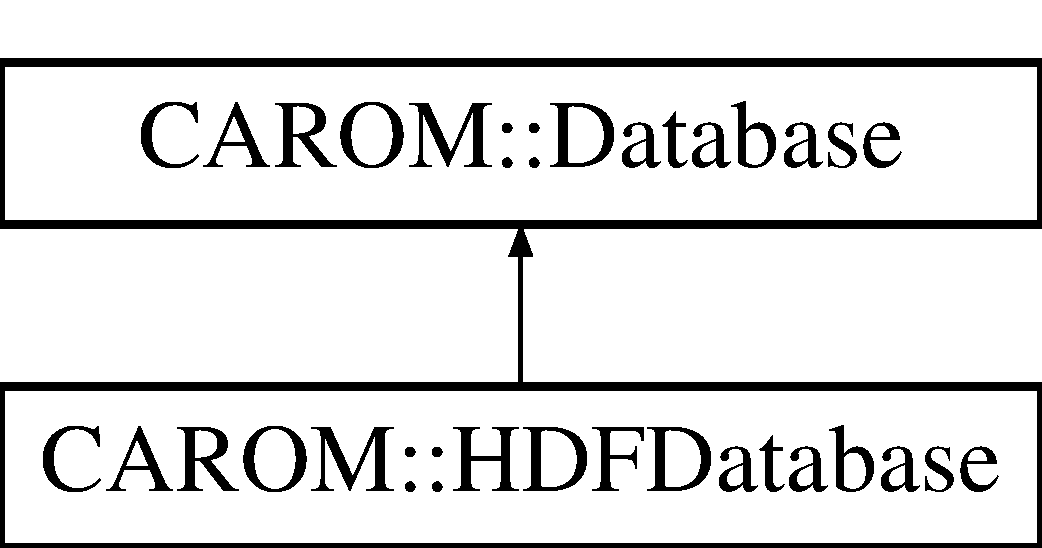
\includegraphics[height=2.000000cm]{class_c_a_r_o_m_1_1_database}
\end{center}
\end{figure}
\subsection*{Public Types}
\begin{DoxyCompactItemize}
\item 
enum \hyperlink{class_c_a_r_o_m_1_1_database_a8ab29ee6466ef8415ee0ef93d94cc5f7}{formats} \{ {\bfseries H\-D\-F5}
 \}
\begin{DoxyCompactList}\small\item\em Implemented database file formats. Add to this enum each time a new database format is implemented. \end{DoxyCompactList}\end{DoxyCompactItemize}
\subsection*{Public Member Functions}
\begin{DoxyCompactItemize}
\item 
\hypertarget{class_c_a_r_o_m_1_1_database_a52d814f0e3f7ab79a7a81df58a269e24}{\hyperlink{class_c_a_r_o_m_1_1_database_a52d814f0e3f7ab79a7a81df58a269e24}{Database} ()}\label{class_c_a_r_o_m_1_1_database_a52d814f0e3f7ab79a7a81df58a269e24}

\begin{DoxyCompactList}\small\item\em Default constructor. \end{DoxyCompactList}\item 
\hypertarget{class_c_a_r_o_m_1_1_database_ac30c27c5448929dd1817475c766e212d}{virtual \hyperlink{class_c_a_r_o_m_1_1_database_ac30c27c5448929dd1817475c766e212d}{$\sim$\-Database} ()}\label{class_c_a_r_o_m_1_1_database_ac30c27c5448929dd1817475c766e212d}

\begin{DoxyCompactList}\small\item\em Destructor. \end{DoxyCompactList}\item 
virtual bool \hyperlink{class_c_a_r_o_m_1_1_database_a5399793945da517596be573c47796223}{create} (const std\-::string \&file\-\_\-name)=0
\begin{DoxyCompactList}\small\item\em Creates a new database file with the supplied name. \end{DoxyCompactList}\item 
virtual bool \hyperlink{class_c_a_r_o_m_1_1_database_a420af85386e4d1aa5f20227116f60f83}{open} (const std\-::string \&file\-\_\-name, const std\-::string \&type)=0
\begin{DoxyCompactList}\small\item\em Opens an existing database file with the supplied name. \end{DoxyCompactList}\item 
virtual bool \hyperlink{class_c_a_r_o_m_1_1_database_a75da8db9a3ffa8c4c150f67e62a600e8}{close} ()=0
\begin{DoxyCompactList}\small\item\em Closes the currently open database file. \end{DoxyCompactList}\item 
void \hyperlink{class_c_a_r_o_m_1_1_database_ab765fefcca1980db5d65f40fd618986d}{put\-Integer} (const std\-::string \&key, int data)
\begin{DoxyCompactList}\small\item\em Writes an integer associated with the supplied key to currently open database file. \end{DoxyCompactList}\item 
virtual void \hyperlink{class_c_a_r_o_m_1_1_database_a3de6b822f53f16bd8fe8eaff2ce520c3}{put\-Integer\-Array} (const std\-::string \&key, const int $\ast$const data, int nelements)=0
\begin{DoxyCompactList}\small\item\em Writes an array of integers associated with the supplied key to the currently open database file. \end{DoxyCompactList}\item 
void \hyperlink{class_c_a_r_o_m_1_1_database_aac3a202671f838713e8d4b5dc47b2dca}{put\-Double} (const std\-::string \&key, double data)
\begin{DoxyCompactList}\small\item\em Writes a double associated with the supplied key to currently open database file. \end{DoxyCompactList}\item 
virtual void \hyperlink{class_c_a_r_o_m_1_1_database_ae85e8cc70193d2802eb73db94fa54975}{put\-Double\-Array} (const std\-::string \&key, const double $\ast$const data, int nelements)=0
\begin{DoxyCompactList}\small\item\em Writes an array of doubles associated with the supplied key to the currently open database file. \end{DoxyCompactList}\item 
void \hyperlink{class_c_a_r_o_m_1_1_database_a5734113f2bec0450fc014f84abdc41c4}{get\-Integer} (const std\-::string \&key, int \&data)
\begin{DoxyCompactList}\small\item\em Reads an integer associated with the supplied key from the currently open database file. \end{DoxyCompactList}\item 
virtual void \hyperlink{class_c_a_r_o_m_1_1_database_a7a518cc3a2b49fbfe70b45030319741d}{get\-Integer\-Array} (const std\-::string \&key, int $\ast$data, int nelements)=0
\begin{DoxyCompactList}\small\item\em Reads an array of integers associated with the supplied key from the currently open database file. \end{DoxyCompactList}\item 
void \hyperlink{class_c_a_r_o_m_1_1_database_aee76ac7276135e202f0d5d6a6adce034}{get\-Double} (const std\-::string \&key, double \&data)
\begin{DoxyCompactList}\small\item\em Reads a double associated with the supplied key from the currently open database file. \end{DoxyCompactList}\item 
virtual void \hyperlink{class_c_a_r_o_m_1_1_database_ab5775af8c9f41f00c4bd8d23227f1b8d}{get\-Double\-Array} (const std\-::string \&key, double $\ast$data, int nelements)=0
\begin{DoxyCompactList}\small\item\em Reads an array of doubles associated with the supplied key from the currently open database file. \end{DoxyCompactList}\end{DoxyCompactItemize}


\subsection{Detailed Description}
Class \hyperlink{class_c_a_r_o_m_1_1_database}{Database} is an abstract base class that provides basic ability to write to and read from a file. It's capabilities are limited to what the \hyperlink{class_c_a_r_o_m_1_1_s_v_d}{S\-V\-D} algorithm needs to read and write its basis vectors. 

\subsection{Member Function Documentation}
\hypertarget{class_c_a_r_o_m_1_1_database_a75da8db9a3ffa8c4c150f67e62a600e8}{\index{C\-A\-R\-O\-M\-::\-Database@{C\-A\-R\-O\-M\-::\-Database}!close@{close}}
\index{close@{close}!CAROM::Database@{C\-A\-R\-O\-M\-::\-Database}}
\subsubsection[{close}]{\setlength{\rightskip}{0pt plus 5cm}virtual bool C\-A\-R\-O\-M\-::\-Database\-::close (
\begin{DoxyParamCaption}
{}
\end{DoxyParamCaption}
)\hspace{0.3cm}{\ttfamily [pure virtual]}}}\label{class_c_a_r_o_m_1_1_database_a75da8db9a3ffa8c4c150f67e62a600e8}


Closes the currently open database file. 

\begin{DoxyReturn}{Returns}
True if the file close was successful. 
\end{DoxyReturn}


Implemented in \hyperlink{class_c_a_r_o_m_1_1_h_d_f_database_a94c9a5972e98e4426c3bdc255ee1dfdc}{C\-A\-R\-O\-M\-::\-H\-D\-F\-Database}.

\hypertarget{class_c_a_r_o_m_1_1_database_a5399793945da517596be573c47796223}{\index{C\-A\-R\-O\-M\-::\-Database@{C\-A\-R\-O\-M\-::\-Database}!create@{create}}
\index{create@{create}!CAROM::Database@{C\-A\-R\-O\-M\-::\-Database}}
\subsubsection[{create}]{\setlength{\rightskip}{0pt plus 5cm}virtual bool C\-A\-R\-O\-M\-::\-Database\-::create (
\begin{DoxyParamCaption}
\item[{const std\-::string \&}]{file\-\_\-name}
\end{DoxyParamCaption}
)\hspace{0.3cm}{\ttfamily [pure virtual]}}}\label{class_c_a_r_o_m_1_1_database_a5399793945da517596be573c47796223}


Creates a new database file with the supplied name. 


\begin{DoxyParams}[1]{Parameters}
\mbox{\tt in}  & {\em file\-\_\-name} & Name of database file to create.\\
\hline
\end{DoxyParams}
\begin{DoxyReturn}{Returns}
True if file create was successful. 
\end{DoxyReturn}


Implemented in \hyperlink{class_c_a_r_o_m_1_1_h_d_f_database_ab86ee99a63cf0259ed1c87d57f3b0960}{C\-A\-R\-O\-M\-::\-H\-D\-F\-Database}.

\hypertarget{class_c_a_r_o_m_1_1_database_aee76ac7276135e202f0d5d6a6adce034}{\index{C\-A\-R\-O\-M\-::\-Database@{C\-A\-R\-O\-M\-::\-Database}!get\-Double@{get\-Double}}
\index{get\-Double@{get\-Double}!CAROM::Database@{C\-A\-R\-O\-M\-::\-Database}}
\subsubsection[{get\-Double}]{\setlength{\rightskip}{0pt plus 5cm}void C\-A\-R\-O\-M\-::\-Database\-::get\-Double (
\begin{DoxyParamCaption}
\item[{const std\-::string \&}]{key, }
\item[{double \&}]{data}
\end{DoxyParamCaption}
)\hspace{0.3cm}{\ttfamily [inline]}}}\label{class_c_a_r_o_m_1_1_database_aee76ac7276135e202f0d5d6a6adce034}


Reads a double associated with the supplied key from the currently open database file. 


\begin{DoxyParams}[1]{Parameters}
\mbox{\tt in}  & {\em key} & The key associated with the value to be read. \\
\hline
\mbox{\tt out}  & {\em data} & The double value read. \\
\hline
\end{DoxyParams}
\hypertarget{class_c_a_r_o_m_1_1_database_ab5775af8c9f41f00c4bd8d23227f1b8d}{\index{C\-A\-R\-O\-M\-::\-Database@{C\-A\-R\-O\-M\-::\-Database}!get\-Double\-Array@{get\-Double\-Array}}
\index{get\-Double\-Array@{get\-Double\-Array}!CAROM::Database@{C\-A\-R\-O\-M\-::\-Database}}
\subsubsection[{get\-Double\-Array}]{\setlength{\rightskip}{0pt plus 5cm}virtual void C\-A\-R\-O\-M\-::\-Database\-::get\-Double\-Array (
\begin{DoxyParamCaption}
\item[{const std\-::string \&}]{key, }
\item[{double $\ast$}]{data, }
\item[{int}]{nelements}
\end{DoxyParamCaption}
)\hspace{0.3cm}{\ttfamily [pure virtual]}}}\label{class_c_a_r_o_m_1_1_database_ab5775af8c9f41f00c4bd8d23227f1b8d}


Reads an array of doubles associated with the supplied key from the currently open database file. 


\begin{DoxyParams}[1]{Parameters}
\mbox{\tt in}  & {\em key} & The key associated with the array of values to be read. \\
\hline
\mbox{\tt out}  & {\em data} & The allocated array of double values to be read. \\
\hline
\mbox{\tt in}  & {\em nelements} & The number of doubles in the array. \\
\hline
\end{DoxyParams}


Implemented in \hyperlink{class_c_a_r_o_m_1_1_h_d_f_database_a0f763843de50277edddc58351ea2f46e}{C\-A\-R\-O\-M\-::\-H\-D\-F\-Database}.

\hypertarget{class_c_a_r_o_m_1_1_database_a5734113f2bec0450fc014f84abdc41c4}{\index{C\-A\-R\-O\-M\-::\-Database@{C\-A\-R\-O\-M\-::\-Database}!get\-Integer@{get\-Integer}}
\index{get\-Integer@{get\-Integer}!CAROM::Database@{C\-A\-R\-O\-M\-::\-Database}}
\subsubsection[{get\-Integer}]{\setlength{\rightskip}{0pt plus 5cm}void C\-A\-R\-O\-M\-::\-Database\-::get\-Integer (
\begin{DoxyParamCaption}
\item[{const std\-::string \&}]{key, }
\item[{int \&}]{data}
\end{DoxyParamCaption}
)\hspace{0.3cm}{\ttfamily [inline]}}}\label{class_c_a_r_o_m_1_1_database_a5734113f2bec0450fc014f84abdc41c4}


Reads an integer associated with the supplied key from the currently open database file. 


\begin{DoxyParams}[1]{Parameters}
\mbox{\tt in}  & {\em key} & The key associated with the value to be read. \\
\hline
\mbox{\tt out}  & {\em data} & The integer value read. \\
\hline
\end{DoxyParams}
\hypertarget{class_c_a_r_o_m_1_1_database_a7a518cc3a2b49fbfe70b45030319741d}{\index{C\-A\-R\-O\-M\-::\-Database@{C\-A\-R\-O\-M\-::\-Database}!get\-Integer\-Array@{get\-Integer\-Array}}
\index{get\-Integer\-Array@{get\-Integer\-Array}!CAROM::Database@{C\-A\-R\-O\-M\-::\-Database}}
\subsubsection[{get\-Integer\-Array}]{\setlength{\rightskip}{0pt plus 5cm}virtual void C\-A\-R\-O\-M\-::\-Database\-::get\-Integer\-Array (
\begin{DoxyParamCaption}
\item[{const std\-::string \&}]{key, }
\item[{int $\ast$}]{data, }
\item[{int}]{nelements}
\end{DoxyParamCaption}
)\hspace{0.3cm}{\ttfamily [pure virtual]}}}\label{class_c_a_r_o_m_1_1_database_a7a518cc3a2b49fbfe70b45030319741d}


Reads an array of integers associated with the supplied key from the currently open database file. 


\begin{DoxyParams}[1]{Parameters}
\mbox{\tt in}  & {\em key} & The key associated with the array of values to be read. \\
\hline
\mbox{\tt out}  & {\em data} & The allocated array of integer values to be read. \\
\hline
\mbox{\tt in}  & {\em nelements} & The number of integers in the array. \\
\hline
\end{DoxyParams}


Implemented in \hyperlink{class_c_a_r_o_m_1_1_h_d_f_database_a9c12c03cef05d3144c21de5f52ff7494}{C\-A\-R\-O\-M\-::\-H\-D\-F\-Database}.

\hypertarget{class_c_a_r_o_m_1_1_database_a420af85386e4d1aa5f20227116f60f83}{\index{C\-A\-R\-O\-M\-::\-Database@{C\-A\-R\-O\-M\-::\-Database}!open@{open}}
\index{open@{open}!CAROM::Database@{C\-A\-R\-O\-M\-::\-Database}}
\subsubsection[{open}]{\setlength{\rightskip}{0pt plus 5cm}virtual bool C\-A\-R\-O\-M\-::\-Database\-::open (
\begin{DoxyParamCaption}
\item[{const std\-::string \&}]{file\-\_\-name, }
\item[{const std\-::string \&}]{type}
\end{DoxyParamCaption}
)\hspace{0.3cm}{\ttfamily [pure virtual]}}}\label{class_c_a_r_o_m_1_1_database_a420af85386e4d1aa5f20227116f60f83}


Opens an existing database file with the supplied name. 


\begin{DoxyParams}[1]{Parameters}
\mbox{\tt in}  & {\em file\-\_\-name} & Name of existing database file to open. \\
\hline
\mbox{\tt in}  & {\em type} & Read/write type (\char`\"{}r\char`\"{}/\char`\"{}wr\char`\"{})\\
\hline
\end{DoxyParams}
\begin{DoxyReturn}{Returns}
True if file open was successful. 
\end{DoxyReturn}


Implemented in \hyperlink{class_c_a_r_o_m_1_1_h_d_f_database_ad221573d351a1f0a2e2356e1a4320089}{C\-A\-R\-O\-M\-::\-H\-D\-F\-Database}.

\hypertarget{class_c_a_r_o_m_1_1_database_aac3a202671f838713e8d4b5dc47b2dca}{\index{C\-A\-R\-O\-M\-::\-Database@{C\-A\-R\-O\-M\-::\-Database}!put\-Double@{put\-Double}}
\index{put\-Double@{put\-Double}!CAROM::Database@{C\-A\-R\-O\-M\-::\-Database}}
\subsubsection[{put\-Double}]{\setlength{\rightskip}{0pt plus 5cm}void C\-A\-R\-O\-M\-::\-Database\-::put\-Double (
\begin{DoxyParamCaption}
\item[{const std\-::string \&}]{key, }
\item[{double}]{data}
\end{DoxyParamCaption}
)\hspace{0.3cm}{\ttfamily [inline]}}}\label{class_c_a_r_o_m_1_1_database_aac3a202671f838713e8d4b5dc47b2dca}


Writes a double associated with the supplied key to currently open database file. 


\begin{DoxyParams}[1]{Parameters}
\mbox{\tt in}  & {\em key} & The key associated with the value to be written. \\
\hline
\mbox{\tt in}  & {\em data} & The double value to be written. \\
\hline
\end{DoxyParams}
\hypertarget{class_c_a_r_o_m_1_1_database_ae85e8cc70193d2802eb73db94fa54975}{\index{C\-A\-R\-O\-M\-::\-Database@{C\-A\-R\-O\-M\-::\-Database}!put\-Double\-Array@{put\-Double\-Array}}
\index{put\-Double\-Array@{put\-Double\-Array}!CAROM::Database@{C\-A\-R\-O\-M\-::\-Database}}
\subsubsection[{put\-Double\-Array}]{\setlength{\rightskip}{0pt plus 5cm}virtual void C\-A\-R\-O\-M\-::\-Database\-::put\-Double\-Array (
\begin{DoxyParamCaption}
\item[{const std\-::string \&}]{key, }
\item[{const double $\ast$const}]{data, }
\item[{int}]{nelements}
\end{DoxyParamCaption}
)\hspace{0.3cm}{\ttfamily [pure virtual]}}}\label{class_c_a_r_o_m_1_1_database_ae85e8cc70193d2802eb73db94fa54975}


Writes an array of doubles associated with the supplied key to the currently open database file. 


\begin{DoxyParams}[1]{Parameters}
\mbox{\tt in}  & {\em key} & The key associated with the array of values to be written. \\
\hline
\mbox{\tt in}  & {\em data} & The array of double values to be written. \\
\hline
\mbox{\tt in}  & {\em nelements} & The number of doubles in the array. \\
\hline
\end{DoxyParams}


Implemented in \hyperlink{class_c_a_r_o_m_1_1_h_d_f_database_ad30894245e7ce642f24be9328b86b91b}{C\-A\-R\-O\-M\-::\-H\-D\-F\-Database}.

\hypertarget{class_c_a_r_o_m_1_1_database_ab765fefcca1980db5d65f40fd618986d}{\index{C\-A\-R\-O\-M\-::\-Database@{C\-A\-R\-O\-M\-::\-Database}!put\-Integer@{put\-Integer}}
\index{put\-Integer@{put\-Integer}!CAROM::Database@{C\-A\-R\-O\-M\-::\-Database}}
\subsubsection[{put\-Integer}]{\setlength{\rightskip}{0pt plus 5cm}void C\-A\-R\-O\-M\-::\-Database\-::put\-Integer (
\begin{DoxyParamCaption}
\item[{const std\-::string \&}]{key, }
\item[{int}]{data}
\end{DoxyParamCaption}
)\hspace{0.3cm}{\ttfamily [inline]}}}\label{class_c_a_r_o_m_1_1_database_ab765fefcca1980db5d65f40fd618986d}


Writes an integer associated with the supplied key to currently open database file. 


\begin{DoxyParams}[1]{Parameters}
\mbox{\tt in}  & {\em key} & The key associated with the value to be written. \\
\hline
\mbox{\tt in}  & {\em data} & The integer value to be written. \\
\hline
\end{DoxyParams}
\hypertarget{class_c_a_r_o_m_1_1_database_a3de6b822f53f16bd8fe8eaff2ce520c3}{\index{C\-A\-R\-O\-M\-::\-Database@{C\-A\-R\-O\-M\-::\-Database}!put\-Integer\-Array@{put\-Integer\-Array}}
\index{put\-Integer\-Array@{put\-Integer\-Array}!CAROM::Database@{C\-A\-R\-O\-M\-::\-Database}}
\subsubsection[{put\-Integer\-Array}]{\setlength{\rightskip}{0pt plus 5cm}virtual void C\-A\-R\-O\-M\-::\-Database\-::put\-Integer\-Array (
\begin{DoxyParamCaption}
\item[{const std\-::string \&}]{key, }
\item[{const int $\ast$const}]{data, }
\item[{int}]{nelements}
\end{DoxyParamCaption}
)\hspace{0.3cm}{\ttfamily [pure virtual]}}}\label{class_c_a_r_o_m_1_1_database_a3de6b822f53f16bd8fe8eaff2ce520c3}


Writes an array of integers associated with the supplied key to the currently open database file. 


\begin{DoxyParams}[1]{Parameters}
\mbox{\tt in}  & {\em key} & The key associated with the array of values to be written. \\
\hline
\mbox{\tt in}  & {\em data} & The array of integer values to be written. \\
\hline
\mbox{\tt in}  & {\em nelements} & The number of integers in the array. \\
\hline
\end{DoxyParams}


Implemented in \hyperlink{class_c_a_r_o_m_1_1_h_d_f_database_a8f628624800817cdbe90ab0407c28305}{C\-A\-R\-O\-M\-::\-H\-D\-F\-Database}.



The documentation for this class was generated from the following file\-:\begin{DoxyCompactItemize}
\item 
Database.\-h\end{DoxyCompactItemize}

\hypertarget{class_c_a_r_o_m_1_1_h_d_f_database}{\section{C\-A\-R\-O\-M\-:\-:H\-D\-F\-Database Class Reference}
\label{class_c_a_r_o_m_1_1_h_d_f_database}\index{C\-A\-R\-O\-M\-::\-H\-D\-F\-Database@{C\-A\-R\-O\-M\-::\-H\-D\-F\-Database}}
}


{\ttfamily \#include $<$H\-D\-F\-Database.\-h$>$}

Inheritance diagram for C\-A\-R\-O\-M\-:\-:H\-D\-F\-Database\-:\begin{figure}[H]
\begin{center}
\leavevmode
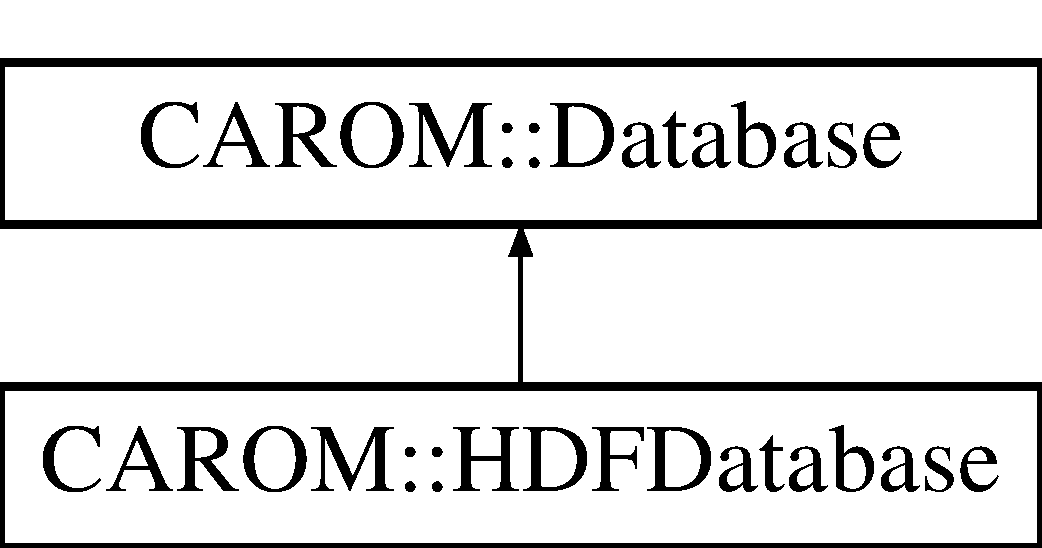
\includegraphics[height=2.000000cm]{class_c_a_r_o_m_1_1_h_d_f_database}
\end{center}
\end{figure}
\subsection*{Public Member Functions}
\begin{DoxyCompactItemize}
\item 
\hypertarget{class_c_a_r_o_m_1_1_h_d_f_database_a99c948a5d96d8b07e66767aff226c3b5}{\hyperlink{class_c_a_r_o_m_1_1_h_d_f_database_a99c948a5d96d8b07e66767aff226c3b5}{H\-D\-F\-Database} ()}\label{class_c_a_r_o_m_1_1_h_d_f_database_a99c948a5d96d8b07e66767aff226c3b5}

\begin{DoxyCompactList}\small\item\em Default constructor. \end{DoxyCompactList}\item 
\hypertarget{class_c_a_r_o_m_1_1_h_d_f_database_a18868c37aa6a37fd6526d56aec2f6f4c}{virtual \hyperlink{class_c_a_r_o_m_1_1_h_d_f_database_a18868c37aa6a37fd6526d56aec2f6f4c}{$\sim$\-H\-D\-F\-Database} ()}\label{class_c_a_r_o_m_1_1_h_d_f_database_a18868c37aa6a37fd6526d56aec2f6f4c}

\begin{DoxyCompactList}\small\item\em Destructor. \end{DoxyCompactList}\item 
virtual bool \hyperlink{class_c_a_r_o_m_1_1_h_d_f_database_ab86ee99a63cf0259ed1c87d57f3b0960}{create} (const std\-::string \&file\-\_\-name)
\begin{DoxyCompactList}\small\item\em Creates a new H\-D\-F5 database file with the supplied name. \end{DoxyCompactList}\item 
virtual bool \hyperlink{class_c_a_r_o_m_1_1_h_d_f_database_ad221573d351a1f0a2e2356e1a4320089}{open} (const std\-::string \&file\-\_\-name, const std\-::string \&type)
\begin{DoxyCompactList}\small\item\em Opens an existing H\-D\-F5 database file with the supplied name. \end{DoxyCompactList}\item 
virtual bool \hyperlink{class_c_a_r_o_m_1_1_h_d_f_database_a94c9a5972e98e4426c3bdc255ee1dfdc}{close} ()
\begin{DoxyCompactList}\small\item\em Closes the currently open H\-D\-F5 database file. \end{DoxyCompactList}\item 
virtual void \hyperlink{class_c_a_r_o_m_1_1_h_d_f_database_a8f628624800817cdbe90ab0407c28305}{put\-Integer\-Array} (const std\-::string \&key, const int $\ast$const data, int nelements)
\begin{DoxyCompactList}\small\item\em Writes an array of integers associated with the supplied key to the currently open H\-D\-F5 database file. \end{DoxyCompactList}\item 
virtual void \hyperlink{class_c_a_r_o_m_1_1_h_d_f_database_ad30894245e7ce642f24be9328b86b91b}{put\-Double\-Array} (const std\-::string \&key, const double $\ast$const data, int nelements)
\begin{DoxyCompactList}\small\item\em Writes an array of doubles associated with the supplied key to the currently open H\-D\-F5 database file. \end{DoxyCompactList}\item 
virtual void \hyperlink{class_c_a_r_o_m_1_1_h_d_f_database_a9c12c03cef05d3144c21de5f52ff7494}{get\-Integer\-Array} (const std\-::string \&key, int $\ast$data, int nelements)
\begin{DoxyCompactList}\small\item\em Reads an array of integers associated with the supplied key from the currently open H\-D\-F5 database file. \end{DoxyCompactList}\item 
virtual void \hyperlink{class_c_a_r_o_m_1_1_h_d_f_database_a0f763843de50277edddc58351ea2f46e}{get\-Double\-Array} (const std\-::string \&key, double $\ast$data, int nelements)
\begin{DoxyCompactList}\small\item\em Reads an array of doubles associated with the supplied key from the currently open H\-D\-F5 database file. \end{DoxyCompactList}\end{DoxyCompactItemize}
\subsection*{Additional Inherited Members}


\subsection{Detailed Description}
\hyperlink{class_c_a_r_o_m_1_1_h_d_f_database}{H\-D\-F\-Database} implements the interface of \hyperlink{class_c_a_r_o_m_1_1_database}{Database} for H\-D\-F5 database files. 

\subsection{Member Function Documentation}
\hypertarget{class_c_a_r_o_m_1_1_h_d_f_database_a94c9a5972e98e4426c3bdc255ee1dfdc}{\index{C\-A\-R\-O\-M\-::\-H\-D\-F\-Database@{C\-A\-R\-O\-M\-::\-H\-D\-F\-Database}!close@{close}}
\index{close@{close}!CAROM::HDFDatabase@{C\-A\-R\-O\-M\-::\-H\-D\-F\-Database}}
\subsubsection[{close}]{\setlength{\rightskip}{0pt plus 5cm}virtual bool C\-A\-R\-O\-M\-::\-H\-D\-F\-Database\-::close (
\begin{DoxyParamCaption}
{}
\end{DoxyParamCaption}
)\hspace{0.3cm}{\ttfamily [virtual]}}}\label{class_c_a_r_o_m_1_1_h_d_f_database_a94c9a5972e98e4426c3bdc255ee1dfdc}


Closes the currently open H\-D\-F5 database file. 

\begin{DoxyReturn}{Returns}
True if the file close was successful. 
\end{DoxyReturn}


Implements \hyperlink{class_c_a_r_o_m_1_1_database_a75da8db9a3ffa8c4c150f67e62a600e8}{C\-A\-R\-O\-M\-::\-Database}.

\hypertarget{class_c_a_r_o_m_1_1_h_d_f_database_ab86ee99a63cf0259ed1c87d57f3b0960}{\index{C\-A\-R\-O\-M\-::\-H\-D\-F\-Database@{C\-A\-R\-O\-M\-::\-H\-D\-F\-Database}!create@{create}}
\index{create@{create}!CAROM::HDFDatabase@{C\-A\-R\-O\-M\-::\-H\-D\-F\-Database}}
\subsubsection[{create}]{\setlength{\rightskip}{0pt plus 5cm}virtual bool C\-A\-R\-O\-M\-::\-H\-D\-F\-Database\-::create (
\begin{DoxyParamCaption}
\item[{const std\-::string \&}]{file\-\_\-name}
\end{DoxyParamCaption}
)\hspace{0.3cm}{\ttfamily [virtual]}}}\label{class_c_a_r_o_m_1_1_h_d_f_database_ab86ee99a63cf0259ed1c87d57f3b0960}


Creates a new H\-D\-F5 database file with the supplied name. 


\begin{DoxyParams}[1]{Parameters}
\mbox{\tt in}  & {\em file\-\_\-name} & Name of H\-D\-F5 database file to create.\\
\hline
\end{DoxyParams}
\begin{DoxyReturn}{Returns}
True if file create was successful. 
\end{DoxyReturn}


Implements \hyperlink{class_c_a_r_o_m_1_1_database_a5399793945da517596be573c47796223}{C\-A\-R\-O\-M\-::\-Database}.

\hypertarget{class_c_a_r_o_m_1_1_h_d_f_database_a0f763843de50277edddc58351ea2f46e}{\index{C\-A\-R\-O\-M\-::\-H\-D\-F\-Database@{C\-A\-R\-O\-M\-::\-H\-D\-F\-Database}!get\-Double\-Array@{get\-Double\-Array}}
\index{get\-Double\-Array@{get\-Double\-Array}!CAROM::HDFDatabase@{C\-A\-R\-O\-M\-::\-H\-D\-F\-Database}}
\subsubsection[{get\-Double\-Array}]{\setlength{\rightskip}{0pt plus 5cm}virtual void C\-A\-R\-O\-M\-::\-H\-D\-F\-Database\-::get\-Double\-Array (
\begin{DoxyParamCaption}
\item[{const std\-::string \&}]{key, }
\item[{double $\ast$}]{data, }
\item[{int}]{nelements}
\end{DoxyParamCaption}
)\hspace{0.3cm}{\ttfamily [virtual]}}}\label{class_c_a_r_o_m_1_1_h_d_f_database_a0f763843de50277edddc58351ea2f46e}


Reads an array of doubles associated with the supplied key from the currently open H\-D\-F5 database file. 

\begin{DoxyPrecond}{Precondition}
!key.empty() 

data != 0 $|$$|$ nelements == 0
\end{DoxyPrecond}

\begin{DoxyParams}[1]{Parameters}
\mbox{\tt in}  & {\em key} & The key associated with the array of values to be read. \\
\hline
\mbox{\tt out}  & {\em data} & The allocated array of double values to be read. \\
\hline
\mbox{\tt in}  & {\em nelements} & The number of doubles in the array. \\
\hline
\end{DoxyParams}


Implements \hyperlink{class_c_a_r_o_m_1_1_database_ab5775af8c9f41f00c4bd8d23227f1b8d}{C\-A\-R\-O\-M\-::\-Database}.

\hypertarget{class_c_a_r_o_m_1_1_h_d_f_database_a9c12c03cef05d3144c21de5f52ff7494}{\index{C\-A\-R\-O\-M\-::\-H\-D\-F\-Database@{C\-A\-R\-O\-M\-::\-H\-D\-F\-Database}!get\-Integer\-Array@{get\-Integer\-Array}}
\index{get\-Integer\-Array@{get\-Integer\-Array}!CAROM::HDFDatabase@{C\-A\-R\-O\-M\-::\-H\-D\-F\-Database}}
\subsubsection[{get\-Integer\-Array}]{\setlength{\rightskip}{0pt plus 5cm}virtual void C\-A\-R\-O\-M\-::\-H\-D\-F\-Database\-::get\-Integer\-Array (
\begin{DoxyParamCaption}
\item[{const std\-::string \&}]{key, }
\item[{int $\ast$}]{data, }
\item[{int}]{nelements}
\end{DoxyParamCaption}
)\hspace{0.3cm}{\ttfamily [virtual]}}}\label{class_c_a_r_o_m_1_1_h_d_f_database_a9c12c03cef05d3144c21de5f52ff7494}


Reads an array of integers associated with the supplied key from the currently open H\-D\-F5 database file. 

\begin{DoxyPrecond}{Precondition}
!key.empty() 

data != 0 $|$$|$ nelements == 0
\end{DoxyPrecond}

\begin{DoxyParams}[1]{Parameters}
\mbox{\tt in}  & {\em key} & The key associated with the array of values to be read. \\
\hline
\mbox{\tt out}  & {\em data} & The allocated array of integer values to be read. \\
\hline
\mbox{\tt in}  & {\em nelements} & The number of integers in the array. \\
\hline
\end{DoxyParams}


Implements \hyperlink{class_c_a_r_o_m_1_1_database_a7a518cc3a2b49fbfe70b45030319741d}{C\-A\-R\-O\-M\-::\-Database}.

\hypertarget{class_c_a_r_o_m_1_1_h_d_f_database_ad221573d351a1f0a2e2356e1a4320089}{\index{C\-A\-R\-O\-M\-::\-H\-D\-F\-Database@{C\-A\-R\-O\-M\-::\-H\-D\-F\-Database}!open@{open}}
\index{open@{open}!CAROM::HDFDatabase@{C\-A\-R\-O\-M\-::\-H\-D\-F\-Database}}
\subsubsection[{open}]{\setlength{\rightskip}{0pt plus 5cm}virtual bool C\-A\-R\-O\-M\-::\-H\-D\-F\-Database\-::open (
\begin{DoxyParamCaption}
\item[{const std\-::string \&}]{file\-\_\-name, }
\item[{const std\-::string \&}]{type}
\end{DoxyParamCaption}
)\hspace{0.3cm}{\ttfamily [virtual]}}}\label{class_c_a_r_o_m_1_1_h_d_f_database_ad221573d351a1f0a2e2356e1a4320089}


Opens an existing H\-D\-F5 database file with the supplied name. 


\begin{DoxyParams}[1]{Parameters}
\mbox{\tt in}  & {\em file\-\_\-name} & Name of existing H\-D\-F5 database file to open. \\
\hline
\mbox{\tt in}  & {\em type} & Read/write type (\char`\"{}r\char`\"{}/\char`\"{}wr\char`\"{})\\
\hline
\end{DoxyParams}
\begin{DoxyReturn}{Returns}
True if file open was successful. 
\end{DoxyReturn}


Implements \hyperlink{class_c_a_r_o_m_1_1_database_a420af85386e4d1aa5f20227116f60f83}{C\-A\-R\-O\-M\-::\-Database}.

\hypertarget{class_c_a_r_o_m_1_1_h_d_f_database_ad30894245e7ce642f24be9328b86b91b}{\index{C\-A\-R\-O\-M\-::\-H\-D\-F\-Database@{C\-A\-R\-O\-M\-::\-H\-D\-F\-Database}!put\-Double\-Array@{put\-Double\-Array}}
\index{put\-Double\-Array@{put\-Double\-Array}!CAROM::HDFDatabase@{C\-A\-R\-O\-M\-::\-H\-D\-F\-Database}}
\subsubsection[{put\-Double\-Array}]{\setlength{\rightskip}{0pt plus 5cm}virtual void C\-A\-R\-O\-M\-::\-H\-D\-F\-Database\-::put\-Double\-Array (
\begin{DoxyParamCaption}
\item[{const std\-::string \&}]{key, }
\item[{const double $\ast$const}]{data, }
\item[{int}]{nelements}
\end{DoxyParamCaption}
)\hspace{0.3cm}{\ttfamily [virtual]}}}\label{class_c_a_r_o_m_1_1_h_d_f_database_ad30894245e7ce642f24be9328b86b91b}


Writes an array of doubles associated with the supplied key to the currently open H\-D\-F5 database file. 

\begin{DoxyPrecond}{Precondition}
!key.empty() 

data != 0 

nelements $>$ 0
\end{DoxyPrecond}

\begin{DoxyParams}[1]{Parameters}
\mbox{\tt in}  & {\em key} & The key associated with the array of values to be written. \\
\hline
\mbox{\tt in}  & {\em data} & The array of double values to be written. \\
\hline
\mbox{\tt in}  & {\em nelements} & The number of doubles in the array. \\
\hline
\end{DoxyParams}


Implements \hyperlink{class_c_a_r_o_m_1_1_database_ae85e8cc70193d2802eb73db94fa54975}{C\-A\-R\-O\-M\-::\-Database}.

\hypertarget{class_c_a_r_o_m_1_1_h_d_f_database_a8f628624800817cdbe90ab0407c28305}{\index{C\-A\-R\-O\-M\-::\-H\-D\-F\-Database@{C\-A\-R\-O\-M\-::\-H\-D\-F\-Database}!put\-Integer\-Array@{put\-Integer\-Array}}
\index{put\-Integer\-Array@{put\-Integer\-Array}!CAROM::HDFDatabase@{C\-A\-R\-O\-M\-::\-H\-D\-F\-Database}}
\subsubsection[{put\-Integer\-Array}]{\setlength{\rightskip}{0pt plus 5cm}virtual void C\-A\-R\-O\-M\-::\-H\-D\-F\-Database\-::put\-Integer\-Array (
\begin{DoxyParamCaption}
\item[{const std\-::string \&}]{key, }
\item[{const int $\ast$const}]{data, }
\item[{int}]{nelements}
\end{DoxyParamCaption}
)\hspace{0.3cm}{\ttfamily [virtual]}}}\label{class_c_a_r_o_m_1_1_h_d_f_database_a8f628624800817cdbe90ab0407c28305}


Writes an array of integers associated with the supplied key to the currently open H\-D\-F5 database file. 

\begin{DoxyPrecond}{Precondition}
!key.empty() 

data != 0 

nelements $>$ 0
\end{DoxyPrecond}

\begin{DoxyParams}[1]{Parameters}
\mbox{\tt in}  & {\em key} & The key associated with the array of values to be written. \\
\hline
\mbox{\tt in}  & {\em data} & The array of integer values to be written. \\
\hline
\mbox{\tt in}  & {\em nelements} & The number of integers in the array. \\
\hline
\end{DoxyParams}


Implements \hyperlink{class_c_a_r_o_m_1_1_database_a3de6b822f53f16bd8fe8eaff2ce520c3}{C\-A\-R\-O\-M\-::\-Database}.



The documentation for this class was generated from the following file\-:\begin{DoxyCompactItemize}
\item 
H\-D\-F\-Database.\-h\end{DoxyCompactItemize}

\hypertarget{class_c_a_r_o_m_1_1_incremental_s_v_d}{\section{C\-A\-R\-O\-M\-:\-:Incremental\-S\-V\-D Class Reference}
\label{class_c_a_r_o_m_1_1_incremental_s_v_d}\index{C\-A\-R\-O\-M\-::\-Incremental\-S\-V\-D@{C\-A\-R\-O\-M\-::\-Incremental\-S\-V\-D}}
}


{\ttfamily \#include $<$Incremental\-S\-V\-D.\-h$>$}

Inheritance diagram for C\-A\-R\-O\-M\-:\-:Incremental\-S\-V\-D\-:\begin{figure}[H]
\begin{center}
\leavevmode
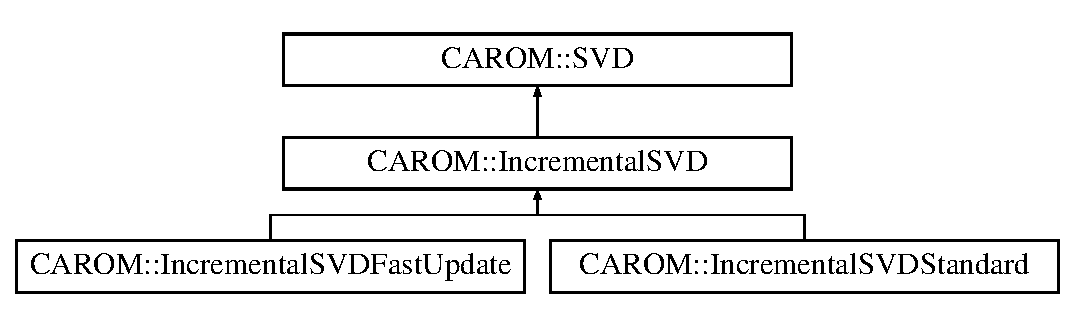
\includegraphics[height=3.000000cm]{class_c_a_r_o_m_1_1_incremental_s_v_d}
\end{center}
\end{figure}
\subsection*{Public Member Functions}
\begin{DoxyCompactItemize}
\item 
\hyperlink{class_c_a_r_o_m_1_1_incremental_s_v_d_ac6ed0c3f346323d614660b7aed97d7f4}{Incremental\-S\-V\-D} (\hyperlink{class_c_a_r_o_m_1_1_options}{Options} options, const std\-::string \&basis\-\_\-file\-\_\-name)
\begin{DoxyCompactList}\small\item\em Constructor. \end{DoxyCompactList}\item 
\hypertarget{class_c_a_r_o_m_1_1_incremental_s_v_d_a6ecab3fd6edb665831c8a7881a4843f0}{virtual \hyperlink{class_c_a_r_o_m_1_1_incremental_s_v_d_a6ecab3fd6edb665831c8a7881a4843f0}{$\sim$\-Incremental\-S\-V\-D} ()}\label{class_c_a_r_o_m_1_1_incremental_s_v_d_a6ecab3fd6edb665831c8a7881a4843f0}

\begin{DoxyCompactList}\small\item\em Destructor. \end{DoxyCompactList}\item 
virtual bool \hyperlink{class_c_a_r_o_m_1_1_incremental_s_v_d_ae9a4f1868de20c86bf1cf06352f9ce6c}{take\-Sample} (double $\ast$u\-\_\-in, double time, bool add\-\_\-without\-\_\-increase=false)
\begin{DoxyCompactList}\small\item\em Sample new state, u\-\_\-in, at the given time. \end{DoxyCompactList}\item 
virtual const \hyperlink{class_c_a_r_o_m_1_1_matrix}{Matrix} $\ast$ \hyperlink{class_c_a_r_o_m_1_1_incremental_s_v_d_a97b0d351b594c3fec9d335bac66c7894}{get\-Spatial\-Basis} ()
\begin{DoxyCompactList}\small\item\em Returns the basis vectors for the current time interval as a \hyperlink{class_c_a_r_o_m_1_1_matrix}{Matrix}. \end{DoxyCompactList}\item 
virtual const \hyperlink{class_c_a_r_o_m_1_1_matrix}{Matrix} $\ast$ \hyperlink{class_c_a_r_o_m_1_1_incremental_s_v_d_a4834472cedc628b07407ef2c0974e69d}{get\-Temporal\-Basis} ()
\begin{DoxyCompactList}\small\item\em Returns the temporal basis vectors for the current time interval as a \hyperlink{class_c_a_r_o_m_1_1_matrix}{Matrix}. \end{DoxyCompactList}\item 
virtual const \hyperlink{class_c_a_r_o_m_1_1_vector}{Vector} $\ast$ \hyperlink{class_c_a_r_o_m_1_1_incremental_s_v_d_a6d5e37fe8e408db06eb01315e0a7586c}{get\-Singular\-Values} ()
\begin{DoxyCompactList}\small\item\em Returns the singular values for the current time interval. \end{DoxyCompactList}\item 
virtual const \hyperlink{class_c_a_r_o_m_1_1_matrix}{Matrix} $\ast$ \hyperlink{class_c_a_r_o_m_1_1_incremental_s_v_d_adaa947ef95ea99f1af5113a9b3461215}{get\-Snapshot\-Matrix} ()
\begin{DoxyCompactList}\small\item\em Returns the snapshot matrix for the current time interval. \end{DoxyCompactList}\end{DoxyCompactItemize}
\subsection*{Protected Member Functions}
\begin{DoxyCompactItemize}
\item 
virtual void \hyperlink{class_c_a_r_o_m_1_1_incremental_s_v_d_a4c079657671bf4d6a281a28f358d38c0}{build\-Initial\-S\-V\-D} (double $\ast$u, double time)=0
\begin{DoxyCompactList}\small\item\em Constructs the first \hyperlink{class_c_a_r_o_m_1_1_s_v_d}{S\-V\-D}. \end{DoxyCompactList}\item 
virtual bool \hyperlink{class_c_a_r_o_m_1_1_incremental_s_v_d_afb79688afbe7988cc5cbd56ec18f8ffb}{build\-Incremental\-S\-V\-D} (double $\ast$u, bool add\-\_\-without\-\_\-increase=false)
\begin{DoxyCompactList}\small\item\em Adds the new sampled the state vector, u, to the system. \end{DoxyCompactList}\item 
\hypertarget{class_c_a_r_o_m_1_1_incremental_s_v_d_a552daa55d3af451c56c00e43625b92b5}{virtual void \hyperlink{class_c_a_r_o_m_1_1_incremental_s_v_d_a552daa55d3af451c56c00e43625b92b5}{compute\-Basis} ()=0}\label{class_c_a_r_o_m_1_1_incremental_s_v_d_a552daa55d3af451c56c00e43625b92b5}

\begin{DoxyCompactList}\small\item\em Computes the current basis vectors. \end{DoxyCompactList}\item 
void \hyperlink{class_c_a_r_o_m_1_1_incremental_s_v_d_a91e61d07d81e6aa52601ec435984919f}{construct\-Q} (double $\ast$\&Q, const \hyperlink{class_c_a_r_o_m_1_1_vector}{Vector} $\ast$l, double k)
\begin{DoxyCompactList}\small\item\em Construct the matrix Q whose \hyperlink{class_c_a_r_o_m_1_1_s_v_d}{S\-V\-D} is needed. \end{DoxyCompactList}\item 
bool \hyperlink{class_c_a_r_o_m_1_1_incremental_s_v_d_aade80460f0cfb9f6b66e07089b647802}{svd} (double $\ast$A, \hyperlink{class_c_a_r_o_m_1_1_matrix}{Matrix} $\ast$\&U, \hyperlink{class_c_a_r_o_m_1_1_matrix}{Matrix} $\ast$\&S, \hyperlink{class_c_a_r_o_m_1_1_matrix}{Matrix} $\ast$\&V)
\begin{DoxyCompactList}\small\item\em Given a matrix, A, returns 2 of the 3 components of its singular value decomposition. The right singular vectors are not needed and therefore not returned. \end{DoxyCompactList}\item 
virtual void \hyperlink{class_c_a_r_o_m_1_1_incremental_s_v_d_adfbd27cfba3479d79d5a4655205d1a3c}{add\-Linearly\-Dependent\-Sample} (const \hyperlink{class_c_a_r_o_m_1_1_matrix}{Matrix} $\ast$A, const \hyperlink{class_c_a_r_o_m_1_1_matrix}{Matrix} $\ast$W, const \hyperlink{class_c_a_r_o_m_1_1_matrix}{Matrix} $\ast$sigma)=0
\begin{DoxyCompactList}\small\item\em Add a linearly dependent sample to the \hyperlink{class_c_a_r_o_m_1_1_s_v_d}{S\-V\-D}. \end{DoxyCompactList}\item 
virtual void \hyperlink{class_c_a_r_o_m_1_1_incremental_s_v_d_a42963b41f3beb65b46d355f93fe3c8e4}{add\-New\-Sample} (const \hyperlink{class_c_a_r_o_m_1_1_vector}{Vector} $\ast$j, const \hyperlink{class_c_a_r_o_m_1_1_matrix}{Matrix} $\ast$A, const \hyperlink{class_c_a_r_o_m_1_1_matrix}{Matrix} $\ast$W, \hyperlink{class_c_a_r_o_m_1_1_matrix}{Matrix} $\ast$sigma)=0
\begin{DoxyCompactList}\small\item\em Add a new, unique sample to the \hyperlink{class_c_a_r_o_m_1_1_s_v_d}{S\-V\-D}. \end{DoxyCompactList}\item 
int \hyperlink{class_c_a_r_o_m_1_1_incremental_s_v_d_a990854bd1eae209a722160647b362109}{num\-Samples} ()
\begin{DoxyCompactList}\small\item\em The number of samples stored. \end{DoxyCompactList}\item 
double \hyperlink{class_c_a_r_o_m_1_1_incremental_s_v_d_a15ff15297ab54cbffb44a86d83655d70}{check\-Orthogonality} (const \hyperlink{class_c_a_r_o_m_1_1_matrix}{Matrix} $\ast$m)
\begin{DoxyCompactList}\small\item\em Computes and returns the orthogonality of m. \end{DoxyCompactList}\item 
void \hyperlink{class_c_a_r_o_m_1_1_incremental_s_v_d_a527589bf79c7ae0636c3bba4a2861b28}{re\-Orthogonalize} (\hyperlink{class_c_a_r_o_m_1_1_matrix}{Matrix} $\ast$m)
\begin{DoxyCompactList}\small\item\em Reorthogonalizes m. \end{DoxyCompactList}\end{DoxyCompactItemize}
\subsection*{Protected Attributes}
\begin{DoxyCompactItemize}
\item 
\hypertarget{class_c_a_r_o_m_1_1_incremental_s_v_d_a3c49e9496b716f451d54e2d2a924717c}{double \hyperlink{class_c_a_r_o_m_1_1_incremental_s_v_d_a3c49e9496b716f451d54e2d2a924717c}{d\-\_\-linearity\-\_\-tol}}\label{class_c_a_r_o_m_1_1_incremental_s_v_d_a3c49e9496b716f451d54e2d2a924717c}

\begin{DoxyCompactList}\small\item\em Tolerance to determine whether or not a sample is linearly dependent. \end{DoxyCompactList}\item 
\hypertarget{class_c_a_r_o_m_1_1_incremental_s_v_d_acec4759c97fae19fe5c468df7d6bab7c}{bool \hyperlink{class_c_a_r_o_m_1_1_incremental_s_v_d_acec4759c97fae19fe5c468df7d6bab7c}{d\-\_\-skip\-\_\-linearly\-\_\-dependent}}\label{class_c_a_r_o_m_1_1_incremental_s_v_d_acec4759c97fae19fe5c468df7d6bab7c}

\begin{DoxyCompactList}\small\item\em Whether to skip linearly dependent samples. \end{DoxyCompactList}\item 
\hypertarget{class_c_a_r_o_m_1_1_incremental_s_v_d_a585fb78a9a58093014220a4e09ae176d}{int \hyperlink{class_c_a_r_o_m_1_1_incremental_s_v_d_a585fb78a9a58093014220a4e09ae176d}{d\-\_\-max\-\_\-basis\-\_\-dimension}}\label{class_c_a_r_o_m_1_1_incremental_s_v_d_a585fb78a9a58093014220a4e09ae176d}

\begin{DoxyCompactList}\small\item\em The maximum basis dimension. \end{DoxyCompactList}\item 
\hypertarget{class_c_a_r_o_m_1_1_incremental_s_v_d_aa208876f1ac66ab10a2be9b0d27f021a}{int \hyperlink{class_c_a_r_o_m_1_1_incremental_s_v_d_aa208876f1ac66ab10a2be9b0d27f021a}{d\-\_\-size}}\label{class_c_a_r_o_m_1_1_incremental_s_v_d_aa208876f1ac66ab10a2be9b0d27f021a}

\begin{DoxyCompactList}\small\item\em The total number of processors. \end{DoxyCompactList}\item 
\hypertarget{class_c_a_r_o_m_1_1_incremental_s_v_d_aeb9834edb3a0424ae3c930945831228d}{int \hyperlink{class_c_a_r_o_m_1_1_incremental_s_v_d_aeb9834edb3a0424ae3c930945831228d}{d\-\_\-rank}}\label{class_c_a_r_o_m_1_1_incremental_s_v_d_aeb9834edb3a0424ae3c930945831228d}

\begin{DoxyCompactList}\small\item\em The rank of the processor owning this object. \end{DoxyCompactList}\item 
\hypertarget{class_c_a_r_o_m_1_1_incremental_s_v_d_a18cefa3fd722cf27bbad6a1b02cb4d5d}{std\-::vector$<$ int $>$ \hyperlink{class_c_a_r_o_m_1_1_incremental_s_v_d_a18cefa3fd722cf27bbad6a1b02cb4d5d}{d\-\_\-proc\-\_\-dims}}\label{class_c_a_r_o_m_1_1_incremental_s_v_d_a18cefa3fd722cf27bbad6a1b02cb4d5d}

\begin{DoxyCompactList}\small\item\em The dimension of the system on each processor. \end{DoxyCompactList}\item 
\hypertarget{class_c_a_r_o_m_1_1_incremental_s_v_d_a64075bb014d7acaca035254ca1b5f4e9}{long int \hyperlink{class_c_a_r_o_m_1_1_incremental_s_v_d_a64075bb014d7acaca035254ca1b5f4e9}{d\-\_\-total\-\_\-dim}}\label{class_c_a_r_o_m_1_1_incremental_s_v_d_a64075bb014d7acaca035254ca1b5f4e9}

\begin{DoxyCompactList}\small\item\em The total dimension of the system. \end{DoxyCompactList}\item 
\hypertarget{class_c_a_r_o_m_1_1_incremental_s_v_d_a0668be92dac1554ceef0eebda70cb512}{bool \hyperlink{class_c_a_r_o_m_1_1_incremental_s_v_d_a0668be92dac1554ceef0eebda70cb512}{d\-\_\-save\-\_\-state}}\label{class_c_a_r_o_m_1_1_incremental_s_v_d_a0668be92dac1554ceef0eebda70cb512}

\begin{DoxyCompactList}\small\item\em If true the state of the \hyperlink{class_c_a_r_o_m_1_1_s_v_d}{S\-V\-D} will be written to disk when the object is deleted. If there are multiple time intervals then the state will not be saved as restoring such a state makes no sense. \end{DoxyCompactList}\item 
\hypertarget{class_c_a_r_o_m_1_1_incremental_s_v_d_a3289b31326d526b985001bf617982e62}{bool \hyperlink{class_c_a_r_o_m_1_1_incremental_s_v_d_a3289b31326d526b985001bf617982e62}{d\-\_\-update\-\_\-right\-\_\-\-S\-V}}\label{class_c_a_r_o_m_1_1_incremental_s_v_d_a3289b31326d526b985001bf617982e62}

\begin{DoxyCompactList}\small\item\em Whether to update the right singular vectors. \end{DoxyCompactList}\item 
\hypertarget{class_c_a_r_o_m_1_1_incremental_s_v_d_a29d5353eb6d9076d162e7359aa85cb7a}{\hyperlink{class_c_a_r_o_m_1_1_database}{Database} $\ast$ \hyperlink{class_c_a_r_o_m_1_1_incremental_s_v_d_a29d5353eb6d9076d162e7359aa85cb7a}{d\-\_\-state\-\_\-database}}\label{class_c_a_r_o_m_1_1_incremental_s_v_d_a29d5353eb6d9076d162e7359aa85cb7a}

\begin{DoxyCompactList}\small\item\em Pointer to the database that will hold saved state data if the state is to be saved. \end{DoxyCompactList}\item 
\hypertarget{class_c_a_r_o_m_1_1_incremental_s_v_d_a744f223bffa3f21c1db1dc2036250ef1}{std\-::string \hyperlink{class_c_a_r_o_m_1_1_incremental_s_v_d_a744f223bffa3f21c1db1dc2036250ef1}{d\-\_\-state\-\_\-file\-\_\-name}}\label{class_c_a_r_o_m_1_1_incremental_s_v_d_a744f223bffa3f21c1db1dc2036250ef1}

\begin{DoxyCompactList}\small\item\em The name of file to which state is saved or restored from. \end{DoxyCompactList}\end{DoxyCompactItemize}
\subsection*{Static Protected Attributes}
\begin{DoxyCompactItemize}
\item 
\hypertarget{class_c_a_r_o_m_1_1_incremental_s_v_d_a4fced260f1783640543bbc9c17cb72fc}{static const int \hyperlink{class_c_a_r_o_m_1_1_incremental_s_v_d_a4fced260f1783640543bbc9c17cb72fc}{C\-O\-M\-M\-U\-N\-I\-C\-A\-T\-E\-\_\-\-U}}\label{class_c_a_r_o_m_1_1_incremental_s_v_d_a4fced260f1783640543bbc9c17cb72fc}

\begin{DoxyCompactList}\small\item\em M\-P\-I message tag. \end{DoxyCompactList}\end{DoxyCompactItemize}


\subsection{Detailed Description}
Abstract class \hyperlink{class_c_a_r_o_m_1_1_incremental_s_v_d}{Incremental\-S\-V\-D} defines the internal A\-P\-I of the incremental \hyperlink{class_c_a_r_o_m_1_1_s_v_d}{S\-V\-D} algorithm. 

\subsection{Constructor \& Destructor Documentation}
\hypertarget{class_c_a_r_o_m_1_1_incremental_s_v_d_ac6ed0c3f346323d614660b7aed97d7f4}{\index{C\-A\-R\-O\-M\-::\-Incremental\-S\-V\-D@{C\-A\-R\-O\-M\-::\-Incremental\-S\-V\-D}!Incremental\-S\-V\-D@{Incremental\-S\-V\-D}}
\index{Incremental\-S\-V\-D@{Incremental\-S\-V\-D}!CAROM::IncrementalSVD@{C\-A\-R\-O\-M\-::\-Incremental\-S\-V\-D}}
\subsubsection[{Incremental\-S\-V\-D}]{\setlength{\rightskip}{0pt plus 5cm}C\-A\-R\-O\-M\-::\-Incremental\-S\-V\-D\-::\-Incremental\-S\-V\-D (
\begin{DoxyParamCaption}
\item[{{\bf Options}}]{options, }
\item[{const std\-::string \&}]{basis\-\_\-file\-\_\-name}
\end{DoxyParamCaption}
)}}\label{class_c_a_r_o_m_1_1_incremental_s_v_d_ac6ed0c3f346323d614660b7aed97d7f4}


Constructor. 


\begin{DoxyParams}[1]{Parameters}
\mbox{\tt in}  & {\em options} & The struct containing the options for this abstract \hyperlink{class_c_a_r_o_m_1_1_s_v_d}{S\-V\-D} class. \\
\hline
\mbox{\tt in}  & {\em basis\-\_\-file\-\_\-name} & The base part of the name of the file containing the basis vectors. Each process will append its process I\-D to this base name. \\
\hline
\end{DoxyParams}
\begin{DoxySeeAlso}{See Also}
\hyperlink{class_c_a_r_o_m_1_1_options}{Options} 
\end{DoxySeeAlso}


\subsection{Member Function Documentation}
\hypertarget{class_c_a_r_o_m_1_1_incremental_s_v_d_adfbd27cfba3479d79d5a4655205d1a3c}{\index{C\-A\-R\-O\-M\-::\-Incremental\-S\-V\-D@{C\-A\-R\-O\-M\-::\-Incremental\-S\-V\-D}!add\-Linearly\-Dependent\-Sample@{add\-Linearly\-Dependent\-Sample}}
\index{add\-Linearly\-Dependent\-Sample@{add\-Linearly\-Dependent\-Sample}!CAROM::IncrementalSVD@{C\-A\-R\-O\-M\-::\-Incremental\-S\-V\-D}}
\subsubsection[{add\-Linearly\-Dependent\-Sample}]{\setlength{\rightskip}{0pt plus 5cm}virtual void C\-A\-R\-O\-M\-::\-Incremental\-S\-V\-D\-::add\-Linearly\-Dependent\-Sample (
\begin{DoxyParamCaption}
\item[{const {\bf Matrix} $\ast$}]{A, }
\item[{const {\bf Matrix} $\ast$}]{W, }
\item[{const {\bf Matrix} $\ast$}]{sigma}
\end{DoxyParamCaption}
)\hspace{0.3cm}{\ttfamily [protected]}, {\ttfamily [pure virtual]}}}\label{class_c_a_r_o_m_1_1_incremental_s_v_d_adfbd27cfba3479d79d5a4655205d1a3c}


Add a linearly dependent sample to the \hyperlink{class_c_a_r_o_m_1_1_s_v_d}{S\-V\-D}. 

\begin{DoxyPrecond}{Precondition}
A != 0 

sigma != 0
\end{DoxyPrecond}

\begin{DoxyParams}[1]{Parameters}
\mbox{\tt in}  & {\em A} & The left singular vectors. \\
\hline
\mbox{\tt in}  & {\em W} & The right singular vectors. \\
\hline
\mbox{\tt in}  & {\em sigma} & The singular values. \\
\hline
\end{DoxyParams}
\hypertarget{class_c_a_r_o_m_1_1_incremental_s_v_d_a42963b41f3beb65b46d355f93fe3c8e4}{\index{C\-A\-R\-O\-M\-::\-Incremental\-S\-V\-D@{C\-A\-R\-O\-M\-::\-Incremental\-S\-V\-D}!add\-New\-Sample@{add\-New\-Sample}}
\index{add\-New\-Sample@{add\-New\-Sample}!CAROM::IncrementalSVD@{C\-A\-R\-O\-M\-::\-Incremental\-S\-V\-D}}
\subsubsection[{add\-New\-Sample}]{\setlength{\rightskip}{0pt plus 5cm}virtual void C\-A\-R\-O\-M\-::\-Incremental\-S\-V\-D\-::add\-New\-Sample (
\begin{DoxyParamCaption}
\item[{const {\bf Vector} $\ast$}]{j, }
\item[{const {\bf Matrix} $\ast$}]{A, }
\item[{const {\bf Matrix} $\ast$}]{W, }
\item[{{\bf Matrix} $\ast$}]{sigma}
\end{DoxyParamCaption}
)\hspace{0.3cm}{\ttfamily [protected]}, {\ttfamily [pure virtual]}}}\label{class_c_a_r_o_m_1_1_incremental_s_v_d_a42963b41f3beb65b46d355f93fe3c8e4}


Add a new, unique sample to the \hyperlink{class_c_a_r_o_m_1_1_s_v_d}{S\-V\-D}. 

\begin{DoxyPrecond}{Precondition}
j != 0 

A != 0 

sigma != 0
\end{DoxyPrecond}

\begin{DoxyParams}[1]{Parameters}
\mbox{\tt in}  & {\em j} & The new column of d\-\_\-\-U. \\
\hline
\mbox{\tt in}  & {\em A} & The left singular vectors. \\
\hline
\mbox{\tt in}  & {\em W} & The right singular vectors. \\
\hline
\mbox{\tt in}  & {\em sigma} & The singular values. \\
\hline
\end{DoxyParams}
\hypertarget{class_c_a_r_o_m_1_1_incremental_s_v_d_afb79688afbe7988cc5cbd56ec18f8ffb}{\index{C\-A\-R\-O\-M\-::\-Incremental\-S\-V\-D@{C\-A\-R\-O\-M\-::\-Incremental\-S\-V\-D}!build\-Incremental\-S\-V\-D@{build\-Incremental\-S\-V\-D}}
\index{build\-Incremental\-S\-V\-D@{build\-Incremental\-S\-V\-D}!CAROM::IncrementalSVD@{C\-A\-R\-O\-M\-::\-Incremental\-S\-V\-D}}
\subsubsection[{build\-Incremental\-S\-V\-D}]{\setlength{\rightskip}{0pt plus 5cm}virtual bool C\-A\-R\-O\-M\-::\-Incremental\-S\-V\-D\-::build\-Incremental\-S\-V\-D (
\begin{DoxyParamCaption}
\item[{double $\ast$}]{u, }
\item[{bool}]{add\-\_\-without\-\_\-increase = {\ttfamily false}}
\end{DoxyParamCaption}
)\hspace{0.3cm}{\ttfamily [protected]}, {\ttfamily [virtual]}}}\label{class_c_a_r_o_m_1_1_incremental_s_v_d_afb79688afbe7988cc5cbd56ec18f8ffb}


Adds the new sampled the state vector, u, to the system. 

\begin{DoxyPrecond}{Precondition}
u != 0
\end{DoxyPrecond}

\begin{DoxyParams}[1]{Parameters}
\mbox{\tt in}  & {\em u} & The new state. \\
\hline
\mbox{\tt in}  & {\em add\-\_\-without\-\_\-increase} & If true, add\-Linearly\-Dependent is invoked.\\
\hline
\end{DoxyParams}
\begin{DoxyReturn}{Returns}
True if building the incremental \hyperlink{class_c_a_r_o_m_1_1_s_v_d}{S\-V\-D} was successful. 
\end{DoxyReturn}
\hypertarget{class_c_a_r_o_m_1_1_incremental_s_v_d_a4c079657671bf4d6a281a28f358d38c0}{\index{C\-A\-R\-O\-M\-::\-Incremental\-S\-V\-D@{C\-A\-R\-O\-M\-::\-Incremental\-S\-V\-D}!build\-Initial\-S\-V\-D@{build\-Initial\-S\-V\-D}}
\index{build\-Initial\-S\-V\-D@{build\-Initial\-S\-V\-D}!CAROM::IncrementalSVD@{C\-A\-R\-O\-M\-::\-Incremental\-S\-V\-D}}
\subsubsection[{build\-Initial\-S\-V\-D}]{\setlength{\rightskip}{0pt plus 5cm}virtual void C\-A\-R\-O\-M\-::\-Incremental\-S\-V\-D\-::build\-Initial\-S\-V\-D (
\begin{DoxyParamCaption}
\item[{double $\ast$}]{u, }
\item[{double}]{time}
\end{DoxyParamCaption}
)\hspace{0.3cm}{\ttfamily [protected]}, {\ttfamily [pure virtual]}}}\label{class_c_a_r_o_m_1_1_incremental_s_v_d_a4c079657671bf4d6a281a28f358d38c0}


Constructs the first \hyperlink{class_c_a_r_o_m_1_1_s_v_d}{S\-V\-D}. 

\begin{DoxyPrecond}{Precondition}
u != 0 

time $>$= 0.\-0
\end{DoxyPrecond}

\begin{DoxyParams}[1]{Parameters}
\mbox{\tt in}  & {\em u} & The first state. \\
\hline
\mbox{\tt in}  & {\em time} & The simulation time for the first state. \\
\hline
\end{DoxyParams}
\hypertarget{class_c_a_r_o_m_1_1_incremental_s_v_d_a15ff15297ab54cbffb44a86d83655d70}{\index{C\-A\-R\-O\-M\-::\-Incremental\-S\-V\-D@{C\-A\-R\-O\-M\-::\-Incremental\-S\-V\-D}!check\-Orthogonality@{check\-Orthogonality}}
\index{check\-Orthogonality@{check\-Orthogonality}!CAROM::IncrementalSVD@{C\-A\-R\-O\-M\-::\-Incremental\-S\-V\-D}}
\subsubsection[{check\-Orthogonality}]{\setlength{\rightskip}{0pt plus 5cm}double C\-A\-R\-O\-M\-::\-Incremental\-S\-V\-D\-::check\-Orthogonality (
\begin{DoxyParamCaption}
\item[{const {\bf Matrix} $\ast$}]{m}
\end{DoxyParamCaption}
)\hspace{0.3cm}{\ttfamily [protected]}}}\label{class_c_a_r_o_m_1_1_incremental_s_v_d_a15ff15297ab54cbffb44a86d83655d70}


Computes and returns the orthogonality of m. 

\begin{DoxyPrecond}{Precondition}
m != 0
\end{DoxyPrecond}

\begin{DoxyParams}[1]{Parameters}
\mbox{\tt in}  & {\em m} & The matrix to check.\\
\hline
\end{DoxyParams}
\begin{DoxyReturn}{Returns}
The orthogonality of m. 
\end{DoxyReturn}
\hypertarget{class_c_a_r_o_m_1_1_incremental_s_v_d_a91e61d07d81e6aa52601ec435984919f}{\index{C\-A\-R\-O\-M\-::\-Incremental\-S\-V\-D@{C\-A\-R\-O\-M\-::\-Incremental\-S\-V\-D}!construct\-Q@{construct\-Q}}
\index{construct\-Q@{construct\-Q}!CAROM::IncrementalSVD@{C\-A\-R\-O\-M\-::\-Incremental\-S\-V\-D}}
\subsubsection[{construct\-Q}]{\setlength{\rightskip}{0pt plus 5cm}void C\-A\-R\-O\-M\-::\-Incremental\-S\-V\-D\-::construct\-Q (
\begin{DoxyParamCaption}
\item[{double $\ast$\&}]{Q, }
\item[{const {\bf Vector} $\ast$}]{l, }
\item[{double}]{k}
\end{DoxyParamCaption}
)\hspace{0.3cm}{\ttfamily [protected]}}}\label{class_c_a_r_o_m_1_1_incremental_s_v_d_a91e61d07d81e6aa52601ec435984919f}


Construct the matrix Q whose \hyperlink{class_c_a_r_o_m_1_1_s_v_d}{S\-V\-D} is needed. 

\begin{DoxyPrecond}{Precondition}
l != 0 

l.\-dim() == \hyperlink{class_c_a_r_o_m_1_1_incremental_s_v_d_a990854bd1eae209a722160647b362109}{num\-Samples()}
\end{DoxyPrecond}

\begin{DoxyParams}[1]{Parameters}
\mbox{\tt out}  & {\em Q} & The matrix to be constructed. \mbox{[}d\-\_\-\-S,l; 0,k\mbox{]} \\
\hline
\mbox{\tt in}  & {\em l} & The last column of Q. \\
\hline
\mbox{\tt in}  & {\em k} & The lower right element of Q. \\
\hline
\end{DoxyParams}
\hypertarget{class_c_a_r_o_m_1_1_incremental_s_v_d_a6d5e37fe8e408db06eb01315e0a7586c}{\index{C\-A\-R\-O\-M\-::\-Incremental\-S\-V\-D@{C\-A\-R\-O\-M\-::\-Incremental\-S\-V\-D}!get\-Singular\-Values@{get\-Singular\-Values}}
\index{get\-Singular\-Values@{get\-Singular\-Values}!CAROM::IncrementalSVD@{C\-A\-R\-O\-M\-::\-Incremental\-S\-V\-D}}
\subsubsection[{get\-Singular\-Values}]{\setlength{\rightskip}{0pt plus 5cm}virtual const {\bf Vector}$\ast$ C\-A\-R\-O\-M\-::\-Incremental\-S\-V\-D\-::get\-Singular\-Values (
\begin{DoxyParamCaption}
{}
\end{DoxyParamCaption}
)\hspace{0.3cm}{\ttfamily [virtual]}}}\label{class_c_a_r_o_m_1_1_incremental_s_v_d_a6d5e37fe8e408db06eb01315e0a7586c}


Returns the singular values for the current time interval. 

\begin{DoxyReturn}{Returns}
The singular values for the current time interval. 
\end{DoxyReturn}


Implements \hyperlink{class_c_a_r_o_m_1_1_s_v_d_ab9bbaa07ffc11ef329be712669a6c95b}{C\-A\-R\-O\-M\-::\-S\-V\-D}.

\hypertarget{class_c_a_r_o_m_1_1_incremental_s_v_d_adaa947ef95ea99f1af5113a9b3461215}{\index{C\-A\-R\-O\-M\-::\-Incremental\-S\-V\-D@{C\-A\-R\-O\-M\-::\-Incremental\-S\-V\-D}!get\-Snapshot\-Matrix@{get\-Snapshot\-Matrix}}
\index{get\-Snapshot\-Matrix@{get\-Snapshot\-Matrix}!CAROM::IncrementalSVD@{C\-A\-R\-O\-M\-::\-Incremental\-S\-V\-D}}
\subsubsection[{get\-Snapshot\-Matrix}]{\setlength{\rightskip}{0pt plus 5cm}virtual const {\bf Matrix}$\ast$ C\-A\-R\-O\-M\-::\-Incremental\-S\-V\-D\-::get\-Snapshot\-Matrix (
\begin{DoxyParamCaption}
{}
\end{DoxyParamCaption}
)\hspace{0.3cm}{\ttfamily [virtual]}}}\label{class_c_a_r_o_m_1_1_incremental_s_v_d_adaa947ef95ea99f1af5113a9b3461215}


Returns the snapshot matrix for the current time interval. 

\begin{DoxyReturn}{Returns}
The snapshot matrix for the current time interval. 
\end{DoxyReturn}


Implements \hyperlink{class_c_a_r_o_m_1_1_s_v_d_a96b482e76d8c8f7278008af4a0bebf85}{C\-A\-R\-O\-M\-::\-S\-V\-D}.

\hypertarget{class_c_a_r_o_m_1_1_incremental_s_v_d_a97b0d351b594c3fec9d335bac66c7894}{\index{C\-A\-R\-O\-M\-::\-Incremental\-S\-V\-D@{C\-A\-R\-O\-M\-::\-Incremental\-S\-V\-D}!get\-Spatial\-Basis@{get\-Spatial\-Basis}}
\index{get\-Spatial\-Basis@{get\-Spatial\-Basis}!CAROM::IncrementalSVD@{C\-A\-R\-O\-M\-::\-Incremental\-S\-V\-D}}
\subsubsection[{get\-Spatial\-Basis}]{\setlength{\rightskip}{0pt plus 5cm}virtual const {\bf Matrix}$\ast$ C\-A\-R\-O\-M\-::\-Incremental\-S\-V\-D\-::get\-Spatial\-Basis (
\begin{DoxyParamCaption}
{}
\end{DoxyParamCaption}
)\hspace{0.3cm}{\ttfamily [virtual]}}}\label{class_c_a_r_o_m_1_1_incremental_s_v_d_a97b0d351b594c3fec9d335bac66c7894}


Returns the basis vectors for the current time interval as a \hyperlink{class_c_a_r_o_m_1_1_matrix}{Matrix}. 

\begin{DoxyReturn}{Returns}
The basis vectors for the current time interval. 
\end{DoxyReturn}


Implements \hyperlink{class_c_a_r_o_m_1_1_s_v_d_ab152d85dfb91958d2265dd54046752dc}{C\-A\-R\-O\-M\-::\-S\-V\-D}.

\hypertarget{class_c_a_r_o_m_1_1_incremental_s_v_d_a4834472cedc628b07407ef2c0974e69d}{\index{C\-A\-R\-O\-M\-::\-Incremental\-S\-V\-D@{C\-A\-R\-O\-M\-::\-Incremental\-S\-V\-D}!get\-Temporal\-Basis@{get\-Temporal\-Basis}}
\index{get\-Temporal\-Basis@{get\-Temporal\-Basis}!CAROM::IncrementalSVD@{C\-A\-R\-O\-M\-::\-Incremental\-S\-V\-D}}
\subsubsection[{get\-Temporal\-Basis}]{\setlength{\rightskip}{0pt plus 5cm}virtual const {\bf Matrix}$\ast$ C\-A\-R\-O\-M\-::\-Incremental\-S\-V\-D\-::get\-Temporal\-Basis (
\begin{DoxyParamCaption}
{}
\end{DoxyParamCaption}
)\hspace{0.3cm}{\ttfamily [virtual]}}}\label{class_c_a_r_o_m_1_1_incremental_s_v_d_a4834472cedc628b07407ef2c0974e69d}


Returns the temporal basis vectors for the current time interval as a \hyperlink{class_c_a_r_o_m_1_1_matrix}{Matrix}. 

\begin{DoxyReturn}{Returns}
The temporal basis vectors for the current time interval. 
\end{DoxyReturn}


Implements \hyperlink{class_c_a_r_o_m_1_1_s_v_d_a42820d67808cad0b5cc2af1590b98ff9}{C\-A\-R\-O\-M\-::\-S\-V\-D}.

\hypertarget{class_c_a_r_o_m_1_1_incremental_s_v_d_a990854bd1eae209a722160647b362109}{\index{C\-A\-R\-O\-M\-::\-Incremental\-S\-V\-D@{C\-A\-R\-O\-M\-::\-Incremental\-S\-V\-D}!num\-Samples@{num\-Samples}}
\index{num\-Samples@{num\-Samples}!CAROM::IncrementalSVD@{C\-A\-R\-O\-M\-::\-Incremental\-S\-V\-D}}
\subsubsection[{num\-Samples}]{\setlength{\rightskip}{0pt plus 5cm}int C\-A\-R\-O\-M\-::\-Incremental\-S\-V\-D\-::num\-Samples (
\begin{DoxyParamCaption}
{}
\end{DoxyParamCaption}
)\hspace{0.3cm}{\ttfamily [inline]}, {\ttfamily [protected]}}}\label{class_c_a_r_o_m_1_1_incremental_s_v_d_a990854bd1eae209a722160647b362109}


The number of samples stored. 

\begin{DoxyReturn}{Returns}
The number of samples stored. 
\end{DoxyReturn}
\hypertarget{class_c_a_r_o_m_1_1_incremental_s_v_d_a527589bf79c7ae0636c3bba4a2861b28}{\index{C\-A\-R\-O\-M\-::\-Incremental\-S\-V\-D@{C\-A\-R\-O\-M\-::\-Incremental\-S\-V\-D}!re\-Orthogonalize@{re\-Orthogonalize}}
\index{re\-Orthogonalize@{re\-Orthogonalize}!CAROM::IncrementalSVD@{C\-A\-R\-O\-M\-::\-Incremental\-S\-V\-D}}
\subsubsection[{re\-Orthogonalize}]{\setlength{\rightskip}{0pt plus 5cm}void C\-A\-R\-O\-M\-::\-Incremental\-S\-V\-D\-::re\-Orthogonalize (
\begin{DoxyParamCaption}
\item[{{\bf Matrix} $\ast$}]{m}
\end{DoxyParamCaption}
)\hspace{0.3cm}{\ttfamily [protected]}}}\label{class_c_a_r_o_m_1_1_incremental_s_v_d_a527589bf79c7ae0636c3bba4a2861b28}


Reorthogonalizes m. 

\begin{DoxyPrecond}{Precondition}
m != 0
\end{DoxyPrecond}

\begin{DoxyParams}[1]{Parameters}
\mbox{\tt in,out}  & {\em m} & The matrix to reorthogonalize. \\
\hline
\end{DoxyParams}
\hypertarget{class_c_a_r_o_m_1_1_incremental_s_v_d_aade80460f0cfb9f6b66e07089b647802}{\index{C\-A\-R\-O\-M\-::\-Incremental\-S\-V\-D@{C\-A\-R\-O\-M\-::\-Incremental\-S\-V\-D}!svd@{svd}}
\index{svd@{svd}!CAROM::IncrementalSVD@{C\-A\-R\-O\-M\-::\-Incremental\-S\-V\-D}}
\subsubsection[{svd}]{\setlength{\rightskip}{0pt plus 5cm}bool C\-A\-R\-O\-M\-::\-Incremental\-S\-V\-D\-::svd (
\begin{DoxyParamCaption}
\item[{double $\ast$}]{A, }
\item[{{\bf Matrix} $\ast$\&}]{U, }
\item[{{\bf Matrix} $\ast$\&}]{S, }
\item[{{\bf Matrix} $\ast$\&}]{V}
\end{DoxyParamCaption}
)\hspace{0.3cm}{\ttfamily [protected]}}}\label{class_c_a_r_o_m_1_1_incremental_s_v_d_aade80460f0cfb9f6b66e07089b647802}


Given a matrix, A, returns 2 of the 3 components of its singular value decomposition. The right singular vectors are not needed and therefore not returned. 

\begin{DoxyPrecond}{Precondition}
A != 0
\end{DoxyPrecond}

\begin{DoxyParams}[1]{Parameters}
\mbox{\tt in}  & {\em A} & The matrix whose \hyperlink{class_c_a_r_o_m_1_1_s_v_d}{S\-V\-D} is needed. \\
\hline
\mbox{\tt out}  & {\em U} & The left singular vectors of A. \\
\hline
\mbox{\tt out}  & {\em S} & The singular values of A. \\
\hline
\mbox{\tt out}  & {\em V} & The right singular vectors of A.\\
\hline
\end{DoxyParams}
\begin{DoxyReturn}{Returns}
True if the \hyperlink{class_c_a_r_o_m_1_1_s_v_d}{S\-V\-D} succeeded. 
\end{DoxyReturn}
\hypertarget{class_c_a_r_o_m_1_1_incremental_s_v_d_ae9a4f1868de20c86bf1cf06352f9ce6c}{\index{C\-A\-R\-O\-M\-::\-Incremental\-S\-V\-D@{C\-A\-R\-O\-M\-::\-Incremental\-S\-V\-D}!take\-Sample@{take\-Sample}}
\index{take\-Sample@{take\-Sample}!CAROM::IncrementalSVD@{C\-A\-R\-O\-M\-::\-Incremental\-S\-V\-D}}
\subsubsection[{take\-Sample}]{\setlength{\rightskip}{0pt plus 5cm}virtual bool C\-A\-R\-O\-M\-::\-Incremental\-S\-V\-D\-::take\-Sample (
\begin{DoxyParamCaption}
\item[{double $\ast$}]{u\-\_\-in, }
\item[{double}]{time, }
\item[{bool}]{add\-\_\-without\-\_\-increase = {\ttfamily false}}
\end{DoxyParamCaption}
)\hspace{0.3cm}{\ttfamily [virtual]}}}\label{class_c_a_r_o_m_1_1_incremental_s_v_d_ae9a4f1868de20c86bf1cf06352f9ce6c}


Sample new state, u\-\_\-in, at the given time. 

\begin{DoxyPrecond}{Precondition}
u\-\_\-in != 0 

time $>$= 0.\-0
\end{DoxyPrecond}

\begin{DoxyParams}[1]{Parameters}
\mbox{\tt in}  & {\em u\-\_\-in} & The state at the specified time. \\
\hline
\mbox{\tt in}  & {\em time} & The simulation time for the state. \\
\hline
\mbox{\tt in}  & {\em add\-\_\-without\-\_\-increase} & If true, add\-Linearly\-Dependent is invoked.\\
\hline
\end{DoxyParams}
\begin{DoxyReturn}{Returns}
True if the sampling was successful. 
\end{DoxyReturn}


Implements \hyperlink{class_c_a_r_o_m_1_1_s_v_d_a5ed8a558690b130c49c2e923cc625769}{C\-A\-R\-O\-M\-::\-S\-V\-D}.



The documentation for this class was generated from the following file\-:\begin{DoxyCompactItemize}
\item 
Incremental\-S\-V\-D.\-h\end{DoxyCompactItemize}

\hypertarget{class_c_a_r_o_m_1_1_incremental_s_v_d_fast_update}{\section{C\-A\-R\-O\-M\-:\-:Incremental\-S\-V\-D\-Fast\-Update Class Reference}
\label{class_c_a_r_o_m_1_1_incremental_s_v_d_fast_update}\index{C\-A\-R\-O\-M\-::\-Incremental\-S\-V\-D\-Fast\-Update@{C\-A\-R\-O\-M\-::\-Incremental\-S\-V\-D\-Fast\-Update}}
}


{\ttfamily \#include $<$Incremental\-S\-V\-D\-Fast\-Update.\-h$>$}

Inheritance diagram for C\-A\-R\-O\-M\-:\-:Incremental\-S\-V\-D\-Fast\-Update\-:\begin{figure}[H]
\begin{center}
\leavevmode
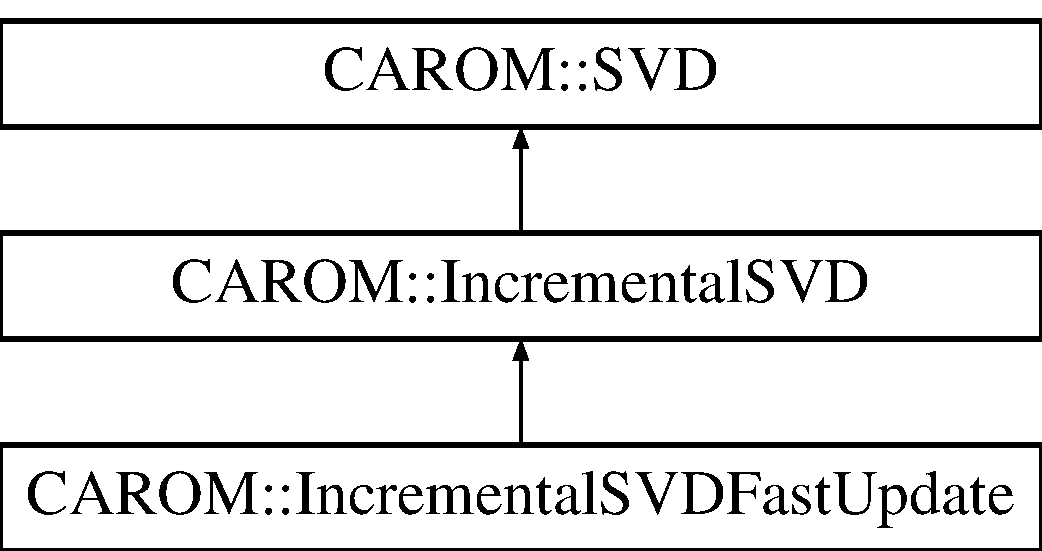
\includegraphics[height=3.000000cm]{class_c_a_r_o_m_1_1_incremental_s_v_d_fast_update}
\end{center}
\end{figure}
\subsection*{Public Member Functions}
\begin{DoxyCompactItemize}
\item 
\hypertarget{class_c_a_r_o_m_1_1_incremental_s_v_d_fast_update_a3d08aaf594df544494e116980c0352fe}{\hyperlink{class_c_a_r_o_m_1_1_incremental_s_v_d_fast_update_a3d08aaf594df544494e116980c0352fe}{$\sim$\-Incremental\-S\-V\-D\-Fast\-Update} ()}\label{class_c_a_r_o_m_1_1_incremental_s_v_d_fast_update_a3d08aaf594df544494e116980c0352fe}

\begin{DoxyCompactList}\small\item\em Destructor. \end{DoxyCompactList}\end{DoxyCompactItemize}
\subsection*{Friends}
\begin{DoxyCompactItemize}
\item 
\hypertarget{class_c_a_r_o_m_1_1_incremental_s_v_d_fast_update_a14677f178902af98cccb02b0058fd326}{class {\bfseries Basis\-Generator}}\label{class_c_a_r_o_m_1_1_incremental_s_v_d_fast_update_a14677f178902af98cccb02b0058fd326}

\end{DoxyCompactItemize}
\subsection*{Additional Inherited Members}


\subsection{Detailed Description}
Class \hyperlink{class_c_a_r_o_m_1_1_incremental_s_v_d_fast_update}{Incremental\-S\-V\-D\-Fast\-Update} implements Brand's fast update incremental \hyperlink{class_c_a_r_o_m_1_1_s_v_d}{S\-V\-D} algorithm by implementing the pure virtual methods of the \hyperlink{class_c_a_r_o_m_1_1_incremental_s_v_d}{Incremental\-S\-V\-D} base class. 

The documentation for this class was generated from the following file\-:\begin{DoxyCompactItemize}
\item 
Incremental\-S\-V\-D\-Fast\-Update.\-h\end{DoxyCompactItemize}

\hypertarget{class_c_a_r_o_m_1_1_incremental_s_v_d_standard}{\section{C\-A\-R\-O\-M\-:\-:Incremental\-S\-V\-D\-Standard Class Reference}
\label{class_c_a_r_o_m_1_1_incremental_s_v_d_standard}\index{C\-A\-R\-O\-M\-::\-Incremental\-S\-V\-D\-Standard@{C\-A\-R\-O\-M\-::\-Incremental\-S\-V\-D\-Standard}}
}


{\ttfamily \#include $<$Incremental\-S\-V\-D\-Standard.\-h$>$}

Inheritance diagram for C\-A\-R\-O\-M\-:\-:Incremental\-S\-V\-D\-Standard\-:\begin{figure}[H]
\begin{center}
\leavevmode
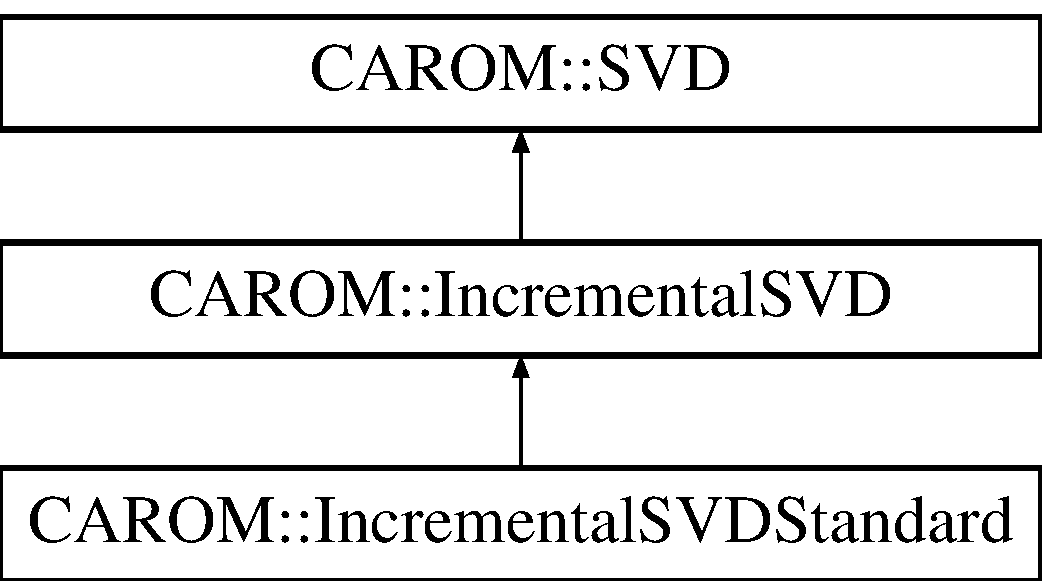
\includegraphics[height=3.000000cm]{class_c_a_r_o_m_1_1_incremental_s_v_d_standard}
\end{center}
\end{figure}
\subsection*{Public Member Functions}
\begin{DoxyCompactItemize}
\item 
\hypertarget{class_c_a_r_o_m_1_1_incremental_s_v_d_standard_a97d171ab198d738d2abb6ea92400ac7f}{\hyperlink{class_c_a_r_o_m_1_1_incremental_s_v_d_standard_a97d171ab198d738d2abb6ea92400ac7f}{$\sim$\-Incremental\-S\-V\-D\-Standard} ()}\label{class_c_a_r_o_m_1_1_incremental_s_v_d_standard_a97d171ab198d738d2abb6ea92400ac7f}

\begin{DoxyCompactList}\small\item\em Destructor. \end{DoxyCompactList}\end{DoxyCompactItemize}
\subsection*{Friends}
\begin{DoxyCompactItemize}
\item 
\hypertarget{class_c_a_r_o_m_1_1_incremental_s_v_d_standard_a14677f178902af98cccb02b0058fd326}{class {\bfseries Basis\-Generator}}\label{class_c_a_r_o_m_1_1_incremental_s_v_d_standard_a14677f178902af98cccb02b0058fd326}

\end{DoxyCompactItemize}
\subsection*{Additional Inherited Members}


\subsection{Detailed Description}
Class \hyperlink{class_c_a_r_o_m_1_1_incremental_s_v_d_standard}{Incremental\-S\-V\-D\-Standard} embodies the standard incremental \hyperlink{class_c_a_r_o_m_1_1_s_v_d}{S\-V\-D} algorithm. 

The documentation for this class was generated from the following file\-:\begin{DoxyCompactItemize}
\item 
Incremental\-S\-V\-D\-Standard.\-h\end{DoxyCompactItemize}

\hypertarget{class_c_a_r_o_m_1_1_matrix}{\section{C\-A\-R\-O\-M\-:\-:Matrix Class Reference}
\label{class_c_a_r_o_m_1_1_matrix}\index{C\-A\-R\-O\-M\-::\-Matrix@{C\-A\-R\-O\-M\-::\-Matrix}}
}


{\ttfamily \#include $<$Matrix.\-h$>$}

\subsection*{Public Member Functions}
\begin{DoxyCompactItemize}
\item 
\hyperlink{class_c_a_r_o_m_1_1_matrix_ad68ec85e555f2ad2f684da50cabd5df6}{Matrix} ()
\item 
\hyperlink{class_c_a_r_o_m_1_1_matrix_aa5c81dbee59703eb959e7e1b6dae2e8b}{Matrix} (int num\-\_\-rows, int num\-\_\-cols, bool \hyperlink{class_c_a_r_o_m_1_1_matrix_a861d3e43b223e8f3217f64a536281605}{distributed}, bool randomized=false)
\item 
\hyperlink{class_c_a_r_o_m_1_1_matrix_afe257256e4912f550567bd1524076807}{Matrix} (double $\ast$mat, int num\-\_\-rows, int num\-\_\-cols, bool \hyperlink{class_c_a_r_o_m_1_1_matrix_a861d3e43b223e8f3217f64a536281605}{distributed}, bool copy\-\_\-data=true)
\item 
\hyperlink{class_c_a_r_o_m_1_1_matrix_abf54e74356673b4139c704eaf9091e4d}{Matrix} (const \hyperlink{class_c_a_r_o_m_1_1_matrix}{Matrix} \&other)
\begin{DoxyCompactList}\small\item\em Copy constructor. \end{DoxyCompactList}\item 
\hypertarget{class_c_a_r_o_m_1_1_matrix_abb5b039c240bdc22ab142ff63fa7f4ba}{\hyperlink{class_c_a_r_o_m_1_1_matrix_abb5b039c240bdc22ab142ff63fa7f4ba}{$\sim$\-Matrix} ()}\label{class_c_a_r_o_m_1_1_matrix_abb5b039c240bdc22ab142ff63fa7f4ba}

\begin{DoxyCompactList}\small\item\em Destructor. \end{DoxyCompactList}\item 
\hyperlink{class_c_a_r_o_m_1_1_matrix}{Matrix} \& \hyperlink{class_c_a_r_o_m_1_1_matrix_a6d8bd9665218767afe7f87abe483996f}{operator=} (const \hyperlink{class_c_a_r_o_m_1_1_matrix}{Matrix} \&rhs)
\begin{DoxyCompactList}\small\item\em Assignment operator. \end{DoxyCompactList}\item 
\hyperlink{class_c_a_r_o_m_1_1_matrix}{Matrix} \& \hyperlink{class_c_a_r_o_m_1_1_matrix_a8e16f2bab44e0c094db4547b6f93d723}{operator=} (const double a)
\begin{DoxyCompactList}\small\item\em Assignment operator. \end{DoxyCompactList}\item 
\hyperlink{class_c_a_r_o_m_1_1_matrix}{Matrix} \& \hyperlink{class_c_a_r_o_m_1_1_matrix_a9eeeaf162c0cbd6a23dd4f00b56b8425}{operator+=} (const \hyperlink{class_c_a_r_o_m_1_1_matrix}{Matrix} \&rhs)
\begin{DoxyCompactList}\small\item\em Addition operator. \end{DoxyCompactList}\item 
\hyperlink{class_c_a_r_o_m_1_1_matrix}{Matrix} \& \hyperlink{class_c_a_r_o_m_1_1_matrix_a916566ad6fcc2ba6eae2a3675e813625}{operator-\/=} (const \hyperlink{class_c_a_r_o_m_1_1_matrix}{Matrix} \&rhs)
\begin{DoxyCompactList}\small\item\em Subtraction operator. \end{DoxyCompactList}\item 
void \hyperlink{class_c_a_r_o_m_1_1_matrix_a0a0305bbb1a56b44c6e2df61152d0a5e}{set\-Size} (int num\-\_\-rows, int num\-\_\-cols)
\begin{DoxyCompactList}\small\item\em Sets the number of rows and columns of the matrix and reallocates storage if needed. \end{DoxyCompactList}\item 
bool \hyperlink{class_c_a_r_o_m_1_1_matrix_a861d3e43b223e8f3217f64a536281605}{distributed} () const 
\begin{DoxyCompactList}\small\item\em Returns true if the \hyperlink{class_c_a_r_o_m_1_1_matrix}{Matrix} is distributed. \end{DoxyCompactList}\item 
\hypertarget{class_c_a_r_o_m_1_1_matrix_aeb1c2a74e21480520dd71cafc7435965}{bool \hyperlink{class_c_a_r_o_m_1_1_matrix_aeb1c2a74e21480520dd71cafc7435965}{balanced} () const }\label{class_c_a_r_o_m_1_1_matrix_aeb1c2a74e21480520dd71cafc7435965}

\begin{DoxyCompactList}\small\item\em Returns true if rows of matrix are load-\/balanced. \end{DoxyCompactList}\item 
int \hyperlink{class_c_a_r_o_m_1_1_matrix_adbda42e4d009f8176b773ec0d87dd665}{num\-Rows} () const 
\begin{DoxyCompactList}\small\item\em Returns the number of rows of the \hyperlink{class_c_a_r_o_m_1_1_matrix}{Matrix} on this processor. \end{DoxyCompactList}\item 
int \hyperlink{class_c_a_r_o_m_1_1_matrix_a1fa97045bd32621d803043ccab7f715f}{num\-Distributed\-Rows} () const 
\begin{DoxyCompactList}\small\item\em Returns the number of rows of the \hyperlink{class_c_a_r_o_m_1_1_matrix}{Matrix} across all processors. \end{DoxyCompactList}\item 
int \hyperlink{class_c_a_r_o_m_1_1_matrix_ac0fae4db551542e9a5cdc401a38fe39f}{num\-Columns} () const 
\begin{DoxyCompactList}\small\item\em Returns the number of columns in the \hyperlink{class_c_a_r_o_m_1_1_matrix}{Matrix}. This method will return the same value from each processor. \end{DoxyCompactList}\item 
\hyperlink{class_c_a_r_o_m_1_1_matrix}{Matrix} $\ast$ \hyperlink{class_c_a_r_o_m_1_1_matrix_a67ae901268ab6138bf2bf9822da4fb10}{mult} (const \hyperlink{class_c_a_r_o_m_1_1_matrix}{Matrix} \&other) const 
\begin{DoxyCompactList}\small\item\em Multiplies this \hyperlink{class_c_a_r_o_m_1_1_matrix}{Matrix} with other and returns the product, reference version. \end{DoxyCompactList}\item 
\hyperlink{class_c_a_r_o_m_1_1_matrix}{Matrix} $\ast$ \hyperlink{class_c_a_r_o_m_1_1_matrix_a5b9c4e3d533410020e65ddc9d85c773d}{mult} (const \hyperlink{class_c_a_r_o_m_1_1_matrix}{Matrix} $\ast$other) const 
\begin{DoxyCompactList}\small\item\em Multiplies this \hyperlink{class_c_a_r_o_m_1_1_matrix}{Matrix} with other and returns the product, pointer version. \end{DoxyCompactList}\item 
void \hyperlink{class_c_a_r_o_m_1_1_matrix_a6f2db8d2f318e733796b3838d7635de1}{mult} (const \hyperlink{class_c_a_r_o_m_1_1_matrix}{Matrix} \&other, \hyperlink{class_c_a_r_o_m_1_1_matrix}{Matrix} $\ast$\&result) const 
\begin{DoxyCompactList}\small\item\em Multiplies this \hyperlink{class_c_a_r_o_m_1_1_matrix}{Matrix} with other and fills result with the answer. \end{DoxyCompactList}\item 
void \hyperlink{class_c_a_r_o_m_1_1_matrix_ab364a0bc6f02142fba687d35bfc7d01b}{mult} (const \hyperlink{class_c_a_r_o_m_1_1_matrix}{Matrix} \&other, \hyperlink{class_c_a_r_o_m_1_1_matrix}{Matrix} \&result) const 
\begin{DoxyCompactList}\small\item\em Multiplies this \hyperlink{class_c_a_r_o_m_1_1_matrix}{Matrix} with other and fills result with the answer. \end{DoxyCompactList}\item 
\hyperlink{class_c_a_r_o_m_1_1_vector}{Vector} $\ast$ \hyperlink{class_c_a_r_o_m_1_1_matrix_ab11e30784d801cd1ef6f972e9c8b88e9}{mult} (const \hyperlink{class_c_a_r_o_m_1_1_vector}{Vector} \&other) const 
\begin{DoxyCompactList}\small\item\em Multiplies this \hyperlink{class_c_a_r_o_m_1_1_matrix}{Matrix} with other and returns the product, reference version. \end{DoxyCompactList}\item 
\hyperlink{class_c_a_r_o_m_1_1_vector}{Vector} $\ast$ \hyperlink{class_c_a_r_o_m_1_1_matrix_a6de8afd0cab59dd0413f84a83bcb0e5c}{mult} (const \hyperlink{class_c_a_r_o_m_1_1_vector}{Vector} $\ast$other) const 
\begin{DoxyCompactList}\small\item\em Multiplies this \hyperlink{class_c_a_r_o_m_1_1_matrix}{Matrix} with other and returns the product, pointer version. \end{DoxyCompactList}\item 
void \hyperlink{class_c_a_r_o_m_1_1_matrix_a29b16fc146fc9fecbae7c01bba737e17}{mult} (const \hyperlink{class_c_a_r_o_m_1_1_vector}{Vector} \&other, \hyperlink{class_c_a_r_o_m_1_1_vector}{Vector} $\ast$\&result) const 
\begin{DoxyCompactList}\small\item\em Multiplies this \hyperlink{class_c_a_r_o_m_1_1_matrix}{Matrix} with other and fills result with the answer. \end{DoxyCompactList}\item 
void \hyperlink{class_c_a_r_o_m_1_1_matrix_acc2c71fe7bf5f24bb6825aebe07bb0b9}{mult} (const \hyperlink{class_c_a_r_o_m_1_1_vector}{Vector} \&other, \hyperlink{class_c_a_r_o_m_1_1_vector}{Vector} \&result) const 
\begin{DoxyCompactList}\small\item\em Multiplies this \hyperlink{class_c_a_r_o_m_1_1_matrix}{Matrix} with other and fills result with the answer. \end{DoxyCompactList}\item 
void \hyperlink{class_c_a_r_o_m_1_1_matrix_a438765b6451b63759c22b39917c128b1}{pointwise\-\_\-mult} (int this\-\_\-row, const \hyperlink{class_c_a_r_o_m_1_1_vector}{Vector} \&other, \hyperlink{class_c_a_r_o_m_1_1_vector}{Vector} \&result) const 
\begin{DoxyCompactList}\small\item\em Multiplies a specified row of this \hyperlink{class_c_a_r_o_m_1_1_matrix}{Matrix} with other pointwise. \end{DoxyCompactList}\item 
void \hyperlink{class_c_a_r_o_m_1_1_matrix_ac97d136a6747467b84ea9b2b389a823d}{pointwise\-\_\-mult} (int this\-\_\-row, \hyperlink{class_c_a_r_o_m_1_1_vector}{Vector} \&other) const 
\begin{DoxyCompactList}\small\item\em Multiplies a specified row of this \hyperlink{class_c_a_r_o_m_1_1_matrix}{Matrix} with other pointwise. This modifies other. \end{DoxyCompactList}\item 
void \hyperlink{class_c_a_r_o_m_1_1_matrix_aeb6c8e1be7ebeaacaf032d7b00e34bcd}{mult\-Plus} (\hyperlink{class_c_a_r_o_m_1_1_vector}{Vector} \&a, const \hyperlink{class_c_a_r_o_m_1_1_vector}{Vector} \&b, double c) const 
\begin{DoxyCompactList}\small\item\em Computes a += this$\ast$b$\ast$c. \end{DoxyCompactList}\item 
\hyperlink{class_c_a_r_o_m_1_1_matrix}{Matrix} $\ast$ \hyperlink{class_c_a_r_o_m_1_1_matrix_ad0e477b50f0747d5c7d1380e9b609ddd}{transpose\-Mult} (const \hyperlink{class_c_a_r_o_m_1_1_matrix}{Matrix} \&other) const 
\begin{DoxyCompactList}\small\item\em Multiplies the transpose of this \hyperlink{class_c_a_r_o_m_1_1_matrix}{Matrix} with other and returns the product, reference version. \end{DoxyCompactList}\item 
\hyperlink{class_c_a_r_o_m_1_1_matrix}{Matrix} $\ast$ \hyperlink{class_c_a_r_o_m_1_1_matrix_ac9f13fd71ea3caced3b42597ada9b7ef}{transpose\-Mult} (const \hyperlink{class_c_a_r_o_m_1_1_matrix}{Matrix} $\ast$other) const 
\begin{DoxyCompactList}\small\item\em Multiplies the transpose of this \hyperlink{class_c_a_r_o_m_1_1_matrix}{Matrix} with other and returns the product, pointer version. \end{DoxyCompactList}\item 
void \hyperlink{class_c_a_r_o_m_1_1_matrix_aef90804ad912c5a779e9bdcb7e995727}{transpose\-Mult} (const \hyperlink{class_c_a_r_o_m_1_1_matrix}{Matrix} \&other, \hyperlink{class_c_a_r_o_m_1_1_matrix}{Matrix} $\ast$\&result) const 
\begin{DoxyCompactList}\small\item\em Multiplies the transpose of this \hyperlink{class_c_a_r_o_m_1_1_matrix}{Matrix} with other and fills result with the answer. \end{DoxyCompactList}\item 
void \hyperlink{class_c_a_r_o_m_1_1_matrix_ae2a0d272c80fbd09370086febf7390d9}{transpose\-Mult} (const \hyperlink{class_c_a_r_o_m_1_1_matrix}{Matrix} \&other, \hyperlink{class_c_a_r_o_m_1_1_matrix}{Matrix} \&result) const 
\begin{DoxyCompactList}\small\item\em Multiplies the transpose of this \hyperlink{class_c_a_r_o_m_1_1_matrix}{Matrix} with other and fills result with the answer. \end{DoxyCompactList}\item 
\hyperlink{class_c_a_r_o_m_1_1_vector}{Vector} $\ast$ \hyperlink{class_c_a_r_o_m_1_1_matrix_a7d1662f706d4eaf8e8b92477ebdb05fa}{transpose\-Mult} (const \hyperlink{class_c_a_r_o_m_1_1_vector}{Vector} \&other) const 
\begin{DoxyCompactList}\small\item\em Multiplies the transpose of this \hyperlink{class_c_a_r_o_m_1_1_matrix}{Matrix} with other and returns the product, reference version. \end{DoxyCompactList}\item 
\hyperlink{class_c_a_r_o_m_1_1_vector}{Vector} $\ast$ \hyperlink{class_c_a_r_o_m_1_1_matrix_a39c61227789aca94eafd288065f13948}{transpose\-Mult} (const \hyperlink{class_c_a_r_o_m_1_1_vector}{Vector} $\ast$other) const 
\begin{DoxyCompactList}\small\item\em Multiplies the transpose of this \hyperlink{class_c_a_r_o_m_1_1_matrix}{Matrix} with other and returns the product, pointer version. \end{DoxyCompactList}\item 
void \hyperlink{class_c_a_r_o_m_1_1_matrix_ae4a76de340d58b627214871b17d0d32c}{transpose\-Mult} (const \hyperlink{class_c_a_r_o_m_1_1_vector}{Vector} \&other, \hyperlink{class_c_a_r_o_m_1_1_vector}{Vector} $\ast$\&result) const 
\begin{DoxyCompactList}\small\item\em Multiplies the transpose of this \hyperlink{class_c_a_r_o_m_1_1_matrix}{Matrix} with other and fills result with the answer. \end{DoxyCompactList}\item 
void \hyperlink{class_c_a_r_o_m_1_1_matrix_a515573e3b012530e6815aea821caf326}{transpose\-Mult} (const \hyperlink{class_c_a_r_o_m_1_1_vector}{Vector} \&other, \hyperlink{class_c_a_r_o_m_1_1_vector}{Vector} \&result) const 
\begin{DoxyCompactList}\small\item\em Multiplies the transpose of this \hyperlink{class_c_a_r_o_m_1_1_matrix}{Matrix} with other and fills result with the answer. \end{DoxyCompactList}\item 
\hyperlink{class_c_a_r_o_m_1_1_matrix}{Matrix} $\ast$ \hyperlink{class_c_a_r_o_m_1_1_matrix_a2a78bfc980b999b4d52e1e6eb599f0de}{inverse} () const 
\begin{DoxyCompactList}\small\item\em Computes and returns the inverse of this. \end{DoxyCompactList}\item 
void \hyperlink{class_c_a_r_o_m_1_1_matrix_a7a84bff8fd51c252a9f544be8d51aca7}{inverse} (\hyperlink{class_c_a_r_o_m_1_1_matrix}{Matrix} $\ast$\&result) const 
\begin{DoxyCompactList}\small\item\em Computes and returns the inverse of this. \end{DoxyCompactList}\item 
void \hyperlink{class_c_a_r_o_m_1_1_matrix_a87881d43ef01d485cb68ecffd3caa4c6}{inverse} (\hyperlink{class_c_a_r_o_m_1_1_matrix}{Matrix} \&result) const 
\begin{DoxyCompactList}\small\item\em Computes and returns the inverse of this. \end{DoxyCompactList}\item 
void \hyperlink{class_c_a_r_o_m_1_1_matrix_ad61ec4327aa2216d06ebcbab31fd0acc}{inverse} ()
\begin{DoxyCompactList}\small\item\em Computes the inverse of this and stores result in this. \end{DoxyCompactList}\item 
\hyperlink{class_c_a_r_o_m_1_1_vector}{Vector} $\ast$ \hyperlink{class_c_a_r_o_m_1_1_matrix_ad293fe4af27e17f0a3f5fbda6a3e887f}{get\-Column} (int column) const 
\begin{DoxyCompactList}\small\item\em Returns a column of the matrix (not owned by \hyperlink{class_c_a_r_o_m_1_1_matrix}{Matrix}). \end{DoxyCompactList}\item 
void \hyperlink{class_c_a_r_o_m_1_1_matrix_a135b1fc98df48adbe7bd6f389742bf7e}{get\-Column} (int column, \hyperlink{class_c_a_r_o_m_1_1_vector}{Vector} $\ast$\&result) const 
\begin{DoxyCompactList}\small\item\em Returns a column of the matrix (not owned by \hyperlink{class_c_a_r_o_m_1_1_matrix}{Matrix}). \end{DoxyCompactList}\item 
void \hyperlink{class_c_a_r_o_m_1_1_matrix_af925d9f3e5e5ad2141179a435df463f9}{get\-Column} (int column, \hyperlink{class_c_a_r_o_m_1_1_vector}{Vector} \&result) const 
\begin{DoxyCompactList}\small\item\em Returns a column of the matrix (not owned by \hyperlink{class_c_a_r_o_m_1_1_matrix}{Matrix}). \end{DoxyCompactList}\item 
void \hyperlink{class_c_a_r_o_m_1_1_matrix_ae3b84c8b1748711319d55bfc086b6f82}{transpose} ()
\begin{DoxyCompactList}\small\item\em Replaces this \hyperlink{class_c_a_r_o_m_1_1_matrix}{Matrix} with its transpose (in place), in the serial square case only. \end{DoxyCompactList}\item 
void \hyperlink{class_c_a_r_o_m_1_1_matrix_a230332a19a32f07abc0d2645c743d009}{transpose\-Pseudoinverse} ()
\begin{DoxyCompactList}\small\item\em Computes the transpose\-Pseudoinverse of this. \end{DoxyCompactList}\item 
void \hyperlink{class_c_a_r_o_m_1_1_matrix_a28a98f195ceee36abc0e652b05ad6c33}{qrcp\-\_\-pivots\-\_\-transpose} (int $\ast$row\-\_\-pivot, int $\ast$row\-\_\-pivot\-\_\-owner, int pivots\-\_\-requested) const 
\begin{DoxyCompactList}\small\item\em Compute the leading \hyperlink{class_c_a_r_o_m_1_1_matrix_ac0fae4db551542e9a5cdc401a38fe39f}{num\-Columns()} column pivots from a Q\-R decomposition with column pivots (Q\-R\-C\-P) of the transpose of this. \end{DoxyCompactList}\item 
const double \& \hyperlink{class_c_a_r_o_m_1_1_matrix_a2abb4e692fb8eaf2fcc6e5d7d0740e76}{item} (int row, int col) const 
\begin{DoxyCompactList}\small\item\em Const \hyperlink{class_c_a_r_o_m_1_1_matrix}{Matrix} member access. \hyperlink{class_c_a_r_o_m_1_1_matrix}{Matrix} data is stored in row-\/major format. \end{DoxyCompactList}\item 
double \& \hyperlink{class_c_a_r_o_m_1_1_matrix_a882026181013920ecd43fb3de00c8c86}{item} (int row, int col)
\begin{DoxyCompactList}\small\item\em Non-\/const \hyperlink{class_c_a_r_o_m_1_1_matrix}{Matrix} member access. \hyperlink{class_c_a_r_o_m_1_1_matrix}{Matrix} data is stored in row-\/major format. \end{DoxyCompactList}\item 
const double \& \hyperlink{class_c_a_r_o_m_1_1_matrix_a4be140c4a974a5591f286872bba00900}{operator()} (int row, int col) const 
\begin{DoxyCompactList}\small\item\em Const \hyperlink{class_c_a_r_o_m_1_1_matrix}{Matrix} member access. \end{DoxyCompactList}\item 
double \& \hyperlink{class_c_a_r_o_m_1_1_matrix_a6881e755c9a08b362157501b4b8349f9}{operator()} (int row, int col)
\begin{DoxyCompactList}\small\item\em Non-\/const \hyperlink{class_c_a_r_o_m_1_1_matrix}{Matrix} member access. \end{DoxyCompactList}\item 
void \hyperlink{class_c_a_r_o_m_1_1_matrix_a8f3c54f1b7d88acb73751cbb904f1162}{print} (const char $\ast$prefix)
\begin{DoxyCompactList}\small\item\em print \hyperlink{class_c_a_r_o_m_1_1_matrix}{Matrix} into (a) ascii file(s). \end{DoxyCompactList}\item 
void \hyperlink{class_c_a_r_o_m_1_1_matrix_ad19dad3788172b6bd5836e606ff071a3}{write} (const std\-::string \&base\-\_\-file\-\_\-name)
\begin{DoxyCompactList}\small\item\em write \hyperlink{class_c_a_r_o_m_1_1_matrix}{Matrix} into (a) H\-D\-F file(s). \end{DoxyCompactList}\item 
void \hyperlink{class_c_a_r_o_m_1_1_matrix_acdc4a8fd238f64d8106b8f1ba8f2384e}{read} (const std\-::string \&base\-\_\-file\-\_\-name)
\begin{DoxyCompactList}\small\item\em read \hyperlink{class_c_a_r_o_m_1_1_matrix}{Matrix} into (a) H\-D\-F file(s). \end{DoxyCompactList}\item 
void \hyperlink{class_c_a_r_o_m_1_1_matrix_a09da21ed0f70b190d5625303ea2d92e4}{local\-\_\-read} (const std\-::string \&base\-\_\-file\-\_\-name, int rank)
\begin{DoxyCompactList}\small\item\em read \hyperlink{class_c_a_r_o_m_1_1_matrix}{Matrix} into (a) H\-D\-F file(s). \end{DoxyCompactList}\item 
\hypertarget{class_c_a_r_o_m_1_1_matrix_a951b1d63fafbc9b4ddd112bd400ca758}{double $\ast$ \hyperlink{class_c_a_r_o_m_1_1_matrix_a951b1d63fafbc9b4ddd112bd400ca758}{get\-Data} () const }\label{class_c_a_r_o_m_1_1_matrix_a951b1d63fafbc9b4ddd112bd400ca758}

\begin{DoxyCompactList}\small\item\em Get the matrix data as a pointer. \end{DoxyCompactList}\end{DoxyCompactItemize}


\subsection{Detailed Description}
Class \hyperlink{class_c_a_r_o_m_1_1_matrix}{Matrix} is a simple matrix class in which the rows may be distributed across multiple processes. This class supports only the basic operations that are needed by the \hyperlink{class_c_a_r_o_m_1_1_s_v_d}{S\-V\-D} library. 

\subsection{Constructor \& Destructor Documentation}
\hypertarget{class_c_a_r_o_m_1_1_matrix_ad68ec85e555f2ad2f684da50cabd5df6}{\index{C\-A\-R\-O\-M\-::\-Matrix@{C\-A\-R\-O\-M\-::\-Matrix}!Matrix@{Matrix}}
\index{Matrix@{Matrix}!CAROM::Matrix@{C\-A\-R\-O\-M\-::\-Matrix}}
\subsubsection[{Matrix}]{\setlength{\rightskip}{0pt plus 5cm}C\-A\-R\-O\-M\-::\-Matrix\-::\-Matrix (
\begin{DoxyParamCaption}
{}
\end{DoxyParamCaption}
)}}\label{class_c_a_r_o_m_1_1_matrix_ad68ec85e555f2ad2f684da50cabd5df6}
Empty Constructor \hypertarget{class_c_a_r_o_m_1_1_matrix_aa5c81dbee59703eb959e7e1b6dae2e8b}{\index{C\-A\-R\-O\-M\-::\-Matrix@{C\-A\-R\-O\-M\-::\-Matrix}!Matrix@{Matrix}}
\index{Matrix@{Matrix}!CAROM::Matrix@{C\-A\-R\-O\-M\-::\-Matrix}}
\subsubsection[{Matrix}]{\setlength{\rightskip}{0pt plus 5cm}C\-A\-R\-O\-M\-::\-Matrix\-::\-Matrix (
\begin{DoxyParamCaption}
\item[{int}]{num\-\_\-rows, }
\item[{int}]{num\-\_\-cols, }
\item[{bool}]{distributed, }
\item[{bool}]{randomized = {\ttfamily false}}
\end{DoxyParamCaption}
)}}\label{class_c_a_r_o_m_1_1_matrix_aa5c81dbee59703eb959e7e1b6dae2e8b}
Constructor creating a \hyperlink{class_c_a_r_o_m_1_1_matrix}{Matrix} with uninitialized values.

\begin{DoxyPrecond}{Precondition}
num\-\_\-rows $>$ 0 

num\-\_\-cols $>$ 0
\end{DoxyPrecond}

\begin{DoxyParams}[1]{Parameters}
\mbox{\tt in}  & {\em num\-\_\-rows} & When undistributed, the total number of rows of the \hyperlink{class_c_a_r_o_m_1_1_matrix}{Matrix}. When distributed, the part of the total number of rows of the \hyperlink{class_c_a_r_o_m_1_1_matrix}{Matrix} on this processor. \\
\hline
\mbox{\tt in}  & {\em num\-\_\-cols} & The total number of columns of the \hyperlink{class_c_a_r_o_m_1_1_matrix}{Matrix}. \\
\hline
\mbox{\tt in}  & {\em distributed} & If true the rows of the \hyperlink{class_c_a_r_o_m_1_1_matrix}{Matrix} are spread over all processors. \\
\hline
\mbox{\tt in}  & {\em randomized} & If true the matrix will be a standard normally distributed random matrix. \\
\hline
\end{DoxyParams}
\hypertarget{class_c_a_r_o_m_1_1_matrix_afe257256e4912f550567bd1524076807}{\index{C\-A\-R\-O\-M\-::\-Matrix@{C\-A\-R\-O\-M\-::\-Matrix}!Matrix@{Matrix}}
\index{Matrix@{Matrix}!CAROM::Matrix@{C\-A\-R\-O\-M\-::\-Matrix}}
\subsubsection[{Matrix}]{\setlength{\rightskip}{0pt plus 5cm}C\-A\-R\-O\-M\-::\-Matrix\-::\-Matrix (
\begin{DoxyParamCaption}
\item[{double $\ast$}]{mat, }
\item[{int}]{num\-\_\-rows, }
\item[{int}]{num\-\_\-cols, }
\item[{bool}]{distributed, }
\item[{bool}]{copy\-\_\-data = {\ttfamily true}}
\end{DoxyParamCaption}
)}}\label{class_c_a_r_o_m_1_1_matrix_afe257256e4912f550567bd1524076807}
Constructor creating a \hyperlink{class_c_a_r_o_m_1_1_matrix}{Matrix} with uninitialized values.

\begin{DoxyPrecond}{Precondition}
mat != 0 

num\-\_\-rows $>$ 0 

num\-\_\-cols $>$ 0
\end{DoxyPrecond}

\begin{DoxyParams}[1]{Parameters}
\mbox{\tt in}  & {\em mat} & The initial values of the \hyperlink{class_c_a_r_o_m_1_1_matrix}{Matrix}. \\
\hline
\mbox{\tt in}  & {\em num\-\_\-rows} & When undistributed, the total number of rows of the \hyperlink{class_c_a_r_o_m_1_1_matrix}{Matrix}. When distributed, the part of the total number of rows of the \hyperlink{class_c_a_r_o_m_1_1_matrix}{Matrix} on this processor. \\
\hline
\mbox{\tt in}  & {\em num\-\_\-cols} & The total number of columns of the \hyperlink{class_c_a_r_o_m_1_1_matrix}{Matrix}. \\
\hline
\mbox{\tt in}  & {\em distributed} & If true the rows of the \hyperlink{class_c_a_r_o_m_1_1_matrix}{Matrix} are spread over all processors. \\
\hline
\mbox{\tt in}  & {\em copy\-\_\-data} & If true the matrix allocates is own storage and copies the contents of mat into its own storage. Otherwise it uses mat as its storage. \\
\hline
\end{DoxyParams}
\hypertarget{class_c_a_r_o_m_1_1_matrix_abf54e74356673b4139c704eaf9091e4d}{\index{C\-A\-R\-O\-M\-::\-Matrix@{C\-A\-R\-O\-M\-::\-Matrix}!Matrix@{Matrix}}
\index{Matrix@{Matrix}!CAROM::Matrix@{C\-A\-R\-O\-M\-::\-Matrix}}
\subsubsection[{Matrix}]{\setlength{\rightskip}{0pt plus 5cm}C\-A\-R\-O\-M\-::\-Matrix\-::\-Matrix (
\begin{DoxyParamCaption}
\item[{const {\bf Matrix} \&}]{other}
\end{DoxyParamCaption}
)}}\label{class_c_a_r_o_m_1_1_matrix_abf54e74356673b4139c704eaf9091e4d}


Copy constructor. 


\begin{DoxyParams}[1]{Parameters}
\mbox{\tt in}  & {\em other} & The \hyperlink{class_c_a_r_o_m_1_1_matrix}{Matrix} to copy. \\
\hline
\end{DoxyParams}


\subsection{Member Function Documentation}
\hypertarget{class_c_a_r_o_m_1_1_matrix_a861d3e43b223e8f3217f64a536281605}{\index{C\-A\-R\-O\-M\-::\-Matrix@{C\-A\-R\-O\-M\-::\-Matrix}!distributed@{distributed}}
\index{distributed@{distributed}!CAROM::Matrix@{C\-A\-R\-O\-M\-::\-Matrix}}
\subsubsection[{distributed}]{\setlength{\rightskip}{0pt plus 5cm}bool C\-A\-R\-O\-M\-::\-Matrix\-::distributed (
\begin{DoxyParamCaption}
{}
\end{DoxyParamCaption}
) const\hspace{0.3cm}{\ttfamily [inline]}}}\label{class_c_a_r_o_m_1_1_matrix_a861d3e43b223e8f3217f64a536281605}


Returns true if the \hyperlink{class_c_a_r_o_m_1_1_matrix}{Matrix} is distributed. 

\begin{DoxyReturn}{Returns}
True if the \hyperlink{class_c_a_r_o_m_1_1_matrix}{Matrix} is distributed. 
\end{DoxyReturn}
\hypertarget{class_c_a_r_o_m_1_1_matrix_ad293fe4af27e17f0a3f5fbda6a3e887f}{\index{C\-A\-R\-O\-M\-::\-Matrix@{C\-A\-R\-O\-M\-::\-Matrix}!get\-Column@{get\-Column}}
\index{get\-Column@{get\-Column}!CAROM::Matrix@{C\-A\-R\-O\-M\-::\-Matrix}}
\subsubsection[{get\-Column}]{\setlength{\rightskip}{0pt plus 5cm}{\bf Vector}$\ast$ C\-A\-R\-O\-M\-::\-Matrix\-::get\-Column (
\begin{DoxyParamCaption}
\item[{int}]{column}
\end{DoxyParamCaption}
) const\hspace{0.3cm}{\ttfamily [inline]}}}\label{class_c_a_r_o_m_1_1_matrix_ad293fe4af27e17f0a3f5fbda6a3e887f}


Returns a column of the matrix (not owned by \hyperlink{class_c_a_r_o_m_1_1_matrix}{Matrix}). 

\begin{DoxyReturn}{Returns}
A column of the matrix (not owned by \hyperlink{class_c_a_r_o_m_1_1_matrix}{Matrix}). 
\end{DoxyReturn}
\hypertarget{class_c_a_r_o_m_1_1_matrix_a135b1fc98df48adbe7bd6f389742bf7e}{\index{C\-A\-R\-O\-M\-::\-Matrix@{C\-A\-R\-O\-M\-::\-Matrix}!get\-Column@{get\-Column}}
\index{get\-Column@{get\-Column}!CAROM::Matrix@{C\-A\-R\-O\-M\-::\-Matrix}}
\subsubsection[{get\-Column}]{\setlength{\rightskip}{0pt plus 5cm}void C\-A\-R\-O\-M\-::\-Matrix\-::get\-Column (
\begin{DoxyParamCaption}
\item[{int}]{column, }
\item[{{\bf Vector} $\ast$\&}]{result}
\end{DoxyParamCaption}
) const}}\label{class_c_a_r_o_m_1_1_matrix_a135b1fc98df48adbe7bd6f389742bf7e}


Returns a column of the matrix (not owned by \hyperlink{class_c_a_r_o_m_1_1_matrix}{Matrix}). 

\begin{DoxyReturn}{Returns}
A column of the matrix (not owned by \hyperlink{class_c_a_r_o_m_1_1_matrix}{Matrix}). 
\end{DoxyReturn}
\hypertarget{class_c_a_r_o_m_1_1_matrix_af925d9f3e5e5ad2141179a435df463f9}{\index{C\-A\-R\-O\-M\-::\-Matrix@{C\-A\-R\-O\-M\-::\-Matrix}!get\-Column@{get\-Column}}
\index{get\-Column@{get\-Column}!CAROM::Matrix@{C\-A\-R\-O\-M\-::\-Matrix}}
\subsubsection[{get\-Column}]{\setlength{\rightskip}{0pt plus 5cm}void C\-A\-R\-O\-M\-::\-Matrix\-::get\-Column (
\begin{DoxyParamCaption}
\item[{int}]{column, }
\item[{{\bf Vector} \&}]{result}
\end{DoxyParamCaption}
) const}}\label{class_c_a_r_o_m_1_1_matrix_af925d9f3e5e5ad2141179a435df463f9}


Returns a column of the matrix (not owned by \hyperlink{class_c_a_r_o_m_1_1_matrix}{Matrix}). 

\begin{DoxyReturn}{Returns}
A column of the matrix (not owned by \hyperlink{class_c_a_r_o_m_1_1_matrix}{Matrix}). 
\end{DoxyReturn}
\hypertarget{class_c_a_r_o_m_1_1_matrix_a2a78bfc980b999b4d52e1e6eb599f0de}{\index{C\-A\-R\-O\-M\-::\-Matrix@{C\-A\-R\-O\-M\-::\-Matrix}!inverse@{inverse}}
\index{inverse@{inverse}!CAROM::Matrix@{C\-A\-R\-O\-M\-::\-Matrix}}
\subsubsection[{inverse}]{\setlength{\rightskip}{0pt plus 5cm}{\bf Matrix}$\ast$ C\-A\-R\-O\-M\-::\-Matrix\-::inverse (
\begin{DoxyParamCaption}
{}
\end{DoxyParamCaption}
) const\hspace{0.3cm}{\ttfamily [inline]}}}\label{class_c_a_r_o_m_1_1_matrix_a2a78bfc980b999b4d52e1e6eb599f0de}


Computes and returns the inverse of this. 

\begin{DoxyPrecond}{Precondition}
!distributed() 

\hyperlink{class_c_a_r_o_m_1_1_matrix_adbda42e4d009f8176b773ec0d87dd665}{num\-Rows()} == \hyperlink{class_c_a_r_o_m_1_1_matrix_ac0fae4db551542e9a5cdc401a38fe39f}{num\-Columns()}
\end{DoxyPrecond}
\begin{DoxyReturn}{Returns}
The inverse of this. 
\end{DoxyReturn}
\hypertarget{class_c_a_r_o_m_1_1_matrix_a7a84bff8fd51c252a9f544be8d51aca7}{\index{C\-A\-R\-O\-M\-::\-Matrix@{C\-A\-R\-O\-M\-::\-Matrix}!inverse@{inverse}}
\index{inverse@{inverse}!CAROM::Matrix@{C\-A\-R\-O\-M\-::\-Matrix}}
\subsubsection[{inverse}]{\setlength{\rightskip}{0pt plus 5cm}void C\-A\-R\-O\-M\-::\-Matrix\-::inverse (
\begin{DoxyParamCaption}
\item[{{\bf Matrix} $\ast$\&}]{result}
\end{DoxyParamCaption}
) const}}\label{class_c_a_r_o_m_1_1_matrix_a7a84bff8fd51c252a9f544be8d51aca7}


Computes and returns the inverse of this. 

If result has not been allocated it will be, otherwise it will be sized accordingly.

\begin{DoxyPrecond}{Precondition}
result == 0 $|$$|$ (!result-\/$>$\hyperlink{class_c_a_r_o_m_1_1_matrix_a861d3e43b223e8f3217f64a536281605}{distributed()} \&\& result-\/$>$\hyperlink{class_c_a_r_o_m_1_1_matrix_adbda42e4d009f8176b773ec0d87dd665}{num\-Rows()} == \hyperlink{class_c_a_r_o_m_1_1_matrix_adbda42e4d009f8176b773ec0d87dd665}{num\-Rows()} \&\& result-\/$>$\hyperlink{class_c_a_r_o_m_1_1_matrix_ac0fae4db551542e9a5cdc401a38fe39f}{num\-Columns()} == \hyperlink{class_c_a_r_o_m_1_1_matrix_ac0fae4db551542e9a5cdc401a38fe39f}{num\-Columns()}) 

!distributed() 

\hyperlink{class_c_a_r_o_m_1_1_matrix_adbda42e4d009f8176b773ec0d87dd665}{num\-Rows()} == \hyperlink{class_c_a_r_o_m_1_1_matrix_ac0fae4db551542e9a5cdc401a38fe39f}{num\-Columns()}
\end{DoxyPrecond}

\begin{DoxyParams}[1]{Parameters}
\mbox{\tt out}  & {\em result} & The inverse of this. \\
\hline
\end{DoxyParams}
\hypertarget{class_c_a_r_o_m_1_1_matrix_a87881d43ef01d485cb68ecffd3caa4c6}{\index{C\-A\-R\-O\-M\-::\-Matrix@{C\-A\-R\-O\-M\-::\-Matrix}!inverse@{inverse}}
\index{inverse@{inverse}!CAROM::Matrix@{C\-A\-R\-O\-M\-::\-Matrix}}
\subsubsection[{inverse}]{\setlength{\rightskip}{0pt plus 5cm}void C\-A\-R\-O\-M\-::\-Matrix\-::inverse (
\begin{DoxyParamCaption}
\item[{{\bf Matrix} \&}]{result}
\end{DoxyParamCaption}
) const}}\label{class_c_a_r_o_m_1_1_matrix_a87881d43ef01d485cb68ecffd3caa4c6}


Computes and returns the inverse of this. 

Result will be sized accordingly.

\begin{DoxyPrecond}{Precondition}
!result.\hyperlink{class_c_a_r_o_m_1_1_matrix_a861d3e43b223e8f3217f64a536281605}{distributed()} \&\& result.\-num\-Rows() == \hyperlink{class_c_a_r_o_m_1_1_matrix_adbda42e4d009f8176b773ec0d87dd665}{num\-Rows()} \&\& result.\-num\-Columns() == \hyperlink{class_c_a_r_o_m_1_1_matrix_ac0fae4db551542e9a5cdc401a38fe39f}{num\-Columns()} 

!distributed() 

\hyperlink{class_c_a_r_o_m_1_1_matrix_adbda42e4d009f8176b773ec0d87dd665}{num\-Rows()} == \hyperlink{class_c_a_r_o_m_1_1_matrix_ac0fae4db551542e9a5cdc401a38fe39f}{num\-Columns()}
\end{DoxyPrecond}

\begin{DoxyParams}[1]{Parameters}
\mbox{\tt out}  & {\em result} & The inverse of this. \\
\hline
\end{DoxyParams}
\hypertarget{class_c_a_r_o_m_1_1_matrix_ad61ec4327aa2216d06ebcbab31fd0acc}{\index{C\-A\-R\-O\-M\-::\-Matrix@{C\-A\-R\-O\-M\-::\-Matrix}!inverse@{inverse}}
\index{inverse@{inverse}!CAROM::Matrix@{C\-A\-R\-O\-M\-::\-Matrix}}
\subsubsection[{inverse}]{\setlength{\rightskip}{0pt plus 5cm}void C\-A\-R\-O\-M\-::\-Matrix\-::inverse (
\begin{DoxyParamCaption}
{}
\end{DoxyParamCaption}
)}}\label{class_c_a_r_o_m_1_1_matrix_ad61ec4327aa2216d06ebcbab31fd0acc}


Computes the inverse of this and stores result in this. 

\begin{DoxyPrecond}{Precondition}
!distributed() 

\hyperlink{class_c_a_r_o_m_1_1_matrix_adbda42e4d009f8176b773ec0d87dd665}{num\-Rows()} == \hyperlink{class_c_a_r_o_m_1_1_matrix_ac0fae4db551542e9a5cdc401a38fe39f}{num\-Columns()} 
\end{DoxyPrecond}
\hypertarget{class_c_a_r_o_m_1_1_matrix_a2abb4e692fb8eaf2fcc6e5d7d0740e76}{\index{C\-A\-R\-O\-M\-::\-Matrix@{C\-A\-R\-O\-M\-::\-Matrix}!item@{item}}
\index{item@{item}!CAROM::Matrix@{C\-A\-R\-O\-M\-::\-Matrix}}
\subsubsection[{item}]{\setlength{\rightskip}{0pt plus 5cm}const double\& C\-A\-R\-O\-M\-::\-Matrix\-::item (
\begin{DoxyParamCaption}
\item[{int}]{row, }
\item[{int}]{col}
\end{DoxyParamCaption}
) const\hspace{0.3cm}{\ttfamily [inline]}}}\label{class_c_a_r_o_m_1_1_matrix_a2abb4e692fb8eaf2fcc6e5d7d0740e76}


Const \hyperlink{class_c_a_r_o_m_1_1_matrix}{Matrix} member access. \hyperlink{class_c_a_r_o_m_1_1_matrix}{Matrix} data is stored in row-\/major format. 

\begin{DoxyPrecond}{Precondition}
(0 $<$= row) \&\& (row $<$ \hyperlink{class_c_a_r_o_m_1_1_matrix_adbda42e4d009f8176b773ec0d87dd665}{num\-Rows()}) 

(0 $<$= col) \&\& (col $<$ \hyperlink{class_c_a_r_o_m_1_1_matrix_ac0fae4db551542e9a5cdc401a38fe39f}{num\-Columns()})
\end{DoxyPrecond}

\begin{DoxyParams}[1]{Parameters}
\mbox{\tt in}  & {\em row} & The row of the \hyperlink{class_c_a_r_o_m_1_1_matrix}{Matrix} value on this processor requested. \\
\hline
\mbox{\tt in}  & {\em col} & The column of the \hyperlink{class_c_a_r_o_m_1_1_matrix}{Matrix} value requested. \\
\hline
\end{DoxyParams}
\hypertarget{class_c_a_r_o_m_1_1_matrix_a882026181013920ecd43fb3de00c8c86}{\index{C\-A\-R\-O\-M\-::\-Matrix@{C\-A\-R\-O\-M\-::\-Matrix}!item@{item}}
\index{item@{item}!CAROM::Matrix@{C\-A\-R\-O\-M\-::\-Matrix}}
\subsubsection[{item}]{\setlength{\rightskip}{0pt plus 5cm}double\& C\-A\-R\-O\-M\-::\-Matrix\-::item (
\begin{DoxyParamCaption}
\item[{int}]{row, }
\item[{int}]{col}
\end{DoxyParamCaption}
)\hspace{0.3cm}{\ttfamily [inline]}}}\label{class_c_a_r_o_m_1_1_matrix_a882026181013920ecd43fb3de00c8c86}


Non-\/const \hyperlink{class_c_a_r_o_m_1_1_matrix}{Matrix} member access. \hyperlink{class_c_a_r_o_m_1_1_matrix}{Matrix} data is stored in row-\/major format. 

Allows constructs of the form mat\mbox{[}i, j\mbox{]} = val;

\begin{DoxyPrecond}{Precondition}
(0 $<$= row) \&\& (row $<$ \hyperlink{class_c_a_r_o_m_1_1_matrix_adbda42e4d009f8176b773ec0d87dd665}{num\-Rows()}) 

(0 $<$= col) \&\& (col $<$ \hyperlink{class_c_a_r_o_m_1_1_matrix_ac0fae4db551542e9a5cdc401a38fe39f}{num\-Columns()})
\end{DoxyPrecond}

\begin{DoxyParams}[1]{Parameters}
\mbox{\tt in}  & {\em row} & The row of the \hyperlink{class_c_a_r_o_m_1_1_matrix}{Matrix} value on this processor requested. \\
\hline
\mbox{\tt in}  & {\em col} & The column of the \hyperlink{class_c_a_r_o_m_1_1_matrix}{Matrix} value requested. \\
\hline
\end{DoxyParams}
\hypertarget{class_c_a_r_o_m_1_1_matrix_a09da21ed0f70b190d5625303ea2d92e4}{\index{C\-A\-R\-O\-M\-::\-Matrix@{C\-A\-R\-O\-M\-::\-Matrix}!local\-\_\-read@{local\-\_\-read}}
\index{local\-\_\-read@{local\-\_\-read}!CAROM::Matrix@{C\-A\-R\-O\-M\-::\-Matrix}}
\subsubsection[{local\-\_\-read}]{\setlength{\rightskip}{0pt plus 5cm}void C\-A\-R\-O\-M\-::\-Matrix\-::local\-\_\-read (
\begin{DoxyParamCaption}
\item[{const std\-::string \&}]{base\-\_\-file\-\_\-name, }
\item[{int}]{rank}
\end{DoxyParamCaption}
)}}\label{class_c_a_r_o_m_1_1_matrix_a09da21ed0f70b190d5625303ea2d92e4}


read \hyperlink{class_c_a_r_o_m_1_1_matrix}{Matrix} into (a) H\-D\-F file(s). 


\begin{DoxyParams}[1]{Parameters}
\mbox{\tt in}  & {\em base\-\_\-file\-\_\-name} & The base part of the file name. \\
\hline
\end{DoxyParams}
\hypertarget{class_c_a_r_o_m_1_1_matrix_a67ae901268ab6138bf2bf9822da4fb10}{\index{C\-A\-R\-O\-M\-::\-Matrix@{C\-A\-R\-O\-M\-::\-Matrix}!mult@{mult}}
\index{mult@{mult}!CAROM::Matrix@{C\-A\-R\-O\-M\-::\-Matrix}}
\subsubsection[{mult}]{\setlength{\rightskip}{0pt plus 5cm}{\bf Matrix}$\ast$ C\-A\-R\-O\-M\-::\-Matrix\-::mult (
\begin{DoxyParamCaption}
\item[{const {\bf Matrix} \&}]{other}
\end{DoxyParamCaption}
) const\hspace{0.3cm}{\ttfamily [inline]}}}\label{class_c_a_r_o_m_1_1_matrix_a67ae901268ab6138bf2bf9822da4fb10}


Multiplies this \hyperlink{class_c_a_r_o_m_1_1_matrix}{Matrix} with other and returns the product, reference version. 

Supports multiplication of two undistributed matrices returning an undistributed \hyperlink{class_c_a_r_o_m_1_1_matrix}{Matrix}, and multiplication of a distributed \hyperlink{class_c_a_r_o_m_1_1_matrix}{Matrix} with an undistributed \hyperlink{class_c_a_r_o_m_1_1_matrix}{Matrix} returning a distributed \hyperlink{class_c_a_r_o_m_1_1_matrix}{Matrix}.

\begin{DoxyPrecond}{Precondition}
!other.\hyperlink{class_c_a_r_o_m_1_1_matrix_a861d3e43b223e8f3217f64a536281605}{distributed()} 

\hyperlink{class_c_a_r_o_m_1_1_matrix_ac0fae4db551542e9a5cdc401a38fe39f}{num\-Columns()} == other.\-num\-Rows()
\end{DoxyPrecond}

\begin{DoxyParams}[1]{Parameters}
\mbox{\tt in}  & {\em other} & The \hyperlink{class_c_a_r_o_m_1_1_matrix}{Matrix} to multiply with this.\\
\hline
\end{DoxyParams}
\begin{DoxyReturn}{Returns}
The product \hyperlink{class_c_a_r_o_m_1_1_matrix}{Matrix}. 
\end{DoxyReturn}
\hypertarget{class_c_a_r_o_m_1_1_matrix_a5b9c4e3d533410020e65ddc9d85c773d}{\index{C\-A\-R\-O\-M\-::\-Matrix@{C\-A\-R\-O\-M\-::\-Matrix}!mult@{mult}}
\index{mult@{mult}!CAROM::Matrix@{C\-A\-R\-O\-M\-::\-Matrix}}
\subsubsection[{mult}]{\setlength{\rightskip}{0pt plus 5cm}{\bf Matrix}$\ast$ C\-A\-R\-O\-M\-::\-Matrix\-::mult (
\begin{DoxyParamCaption}
\item[{const {\bf Matrix} $\ast$}]{other}
\end{DoxyParamCaption}
) const\hspace{0.3cm}{\ttfamily [inline]}}}\label{class_c_a_r_o_m_1_1_matrix_a5b9c4e3d533410020e65ddc9d85c773d}


Multiplies this \hyperlink{class_c_a_r_o_m_1_1_matrix}{Matrix} with other and returns the product, pointer version. 

Supports multiplication of two undistributed matrices returning an undistributed \hyperlink{class_c_a_r_o_m_1_1_matrix}{Matrix}, and multiplication of a distributed \hyperlink{class_c_a_r_o_m_1_1_matrix}{Matrix} with an undistributed \hyperlink{class_c_a_r_o_m_1_1_matrix}{Matrix} returning a distributed \hyperlink{class_c_a_r_o_m_1_1_matrix}{Matrix}.

\begin{DoxyPrecond}{Precondition}
other != 0 

!other-\/$>$\hyperlink{class_c_a_r_o_m_1_1_matrix_a861d3e43b223e8f3217f64a536281605}{distributed()} 

\hyperlink{class_c_a_r_o_m_1_1_matrix_ac0fae4db551542e9a5cdc401a38fe39f}{num\-Columns()} == other-\/$>$\hyperlink{class_c_a_r_o_m_1_1_matrix_adbda42e4d009f8176b773ec0d87dd665}{num\-Rows()}
\end{DoxyPrecond}

\begin{DoxyParams}[1]{Parameters}
\mbox{\tt in}  & {\em other} & The \hyperlink{class_c_a_r_o_m_1_1_matrix}{Matrix} to multiply with this.\\
\hline
\end{DoxyParams}
\begin{DoxyReturn}{Returns}
The product \hyperlink{class_c_a_r_o_m_1_1_matrix}{Matrix}. 
\end{DoxyReturn}
\hypertarget{class_c_a_r_o_m_1_1_matrix_a6f2db8d2f318e733796b3838d7635de1}{\index{C\-A\-R\-O\-M\-::\-Matrix@{C\-A\-R\-O\-M\-::\-Matrix}!mult@{mult}}
\index{mult@{mult}!CAROM::Matrix@{C\-A\-R\-O\-M\-::\-Matrix}}
\subsubsection[{mult}]{\setlength{\rightskip}{0pt plus 5cm}void C\-A\-R\-O\-M\-::\-Matrix\-::mult (
\begin{DoxyParamCaption}
\item[{const {\bf Matrix} \&}]{other, }
\item[{{\bf Matrix} $\ast$\&}]{result}
\end{DoxyParamCaption}
) const}}\label{class_c_a_r_o_m_1_1_matrix_a6f2db8d2f318e733796b3838d7635de1}


Multiplies this \hyperlink{class_c_a_r_o_m_1_1_matrix}{Matrix} with other and fills result with the answer. 

Supports multiplication of two undistributed matrices resulting in an undistributed \hyperlink{class_c_a_r_o_m_1_1_matrix}{Matrix}, and multiplication of a distributed \hyperlink{class_c_a_r_o_m_1_1_matrix}{Matrix} with an undistributed \hyperlink{class_c_a_r_o_m_1_1_matrix}{Matrix} resulting in a distributed \hyperlink{class_c_a_r_o_m_1_1_matrix}{Matrix}. If result has not been allocated it will be, otherwise it will be sized accordingly.

\begin{DoxyPrecond}{Precondition}
result == 0 $|$$|$ result-\/$>$\hyperlink{class_c_a_r_o_m_1_1_matrix_a861d3e43b223e8f3217f64a536281605}{distributed()} == \hyperlink{class_c_a_r_o_m_1_1_matrix_a861d3e43b223e8f3217f64a536281605}{distributed()} 

!other.\hyperlink{class_c_a_r_o_m_1_1_matrix_a861d3e43b223e8f3217f64a536281605}{distributed()} 

\hyperlink{class_c_a_r_o_m_1_1_matrix_ac0fae4db551542e9a5cdc401a38fe39f}{num\-Columns()} == other.\-num\-Rows()
\end{DoxyPrecond}

\begin{DoxyParams}[1]{Parameters}
\mbox{\tt in}  & {\em other} & The \hyperlink{class_c_a_r_o_m_1_1_matrix}{Matrix} to multiply with this. \\
\hline
\mbox{\tt out}  & {\em result} & The product \hyperlink{class_c_a_r_o_m_1_1_matrix}{Matrix}. \\
\hline
\end{DoxyParams}
\hypertarget{class_c_a_r_o_m_1_1_matrix_ab364a0bc6f02142fba687d35bfc7d01b}{\index{C\-A\-R\-O\-M\-::\-Matrix@{C\-A\-R\-O\-M\-::\-Matrix}!mult@{mult}}
\index{mult@{mult}!CAROM::Matrix@{C\-A\-R\-O\-M\-::\-Matrix}}
\subsubsection[{mult}]{\setlength{\rightskip}{0pt plus 5cm}void C\-A\-R\-O\-M\-::\-Matrix\-::mult (
\begin{DoxyParamCaption}
\item[{const {\bf Matrix} \&}]{other, }
\item[{{\bf Matrix} \&}]{result}
\end{DoxyParamCaption}
) const}}\label{class_c_a_r_o_m_1_1_matrix_ab364a0bc6f02142fba687d35bfc7d01b}


Multiplies this \hyperlink{class_c_a_r_o_m_1_1_matrix}{Matrix} with other and fills result with the answer. 

Supports multiplication of two undistributed matrices resulting in an undistributed \hyperlink{class_c_a_r_o_m_1_1_matrix}{Matrix}, and multiplication of a distributed \hyperlink{class_c_a_r_o_m_1_1_matrix}{Matrix} with an undistributed \hyperlink{class_c_a_r_o_m_1_1_matrix}{Matrix} resulting in a distributed \hyperlink{class_c_a_r_o_m_1_1_matrix}{Matrix}. Result will be sized accordingly.

\begin{DoxyPrecond}{Precondition}
result.\-distributed() == \hyperlink{class_c_a_r_o_m_1_1_matrix_a861d3e43b223e8f3217f64a536281605}{distributed()} 

!other.\hyperlink{class_c_a_r_o_m_1_1_matrix_a861d3e43b223e8f3217f64a536281605}{distributed()} 

\hyperlink{class_c_a_r_o_m_1_1_matrix_ac0fae4db551542e9a5cdc401a38fe39f}{num\-Columns()} == other.\-num\-Rows()
\end{DoxyPrecond}

\begin{DoxyParams}[1]{Parameters}
\mbox{\tt in}  & {\em other} & The \hyperlink{class_c_a_r_o_m_1_1_matrix}{Matrix} to multiply with this. \\
\hline
\mbox{\tt out}  & {\em result} & The product \hyperlink{class_c_a_r_o_m_1_1_matrix}{Matrix}. \\
\hline
\end{DoxyParams}
\hypertarget{class_c_a_r_o_m_1_1_matrix_ab11e30784d801cd1ef6f972e9c8b88e9}{\index{C\-A\-R\-O\-M\-::\-Matrix@{C\-A\-R\-O\-M\-::\-Matrix}!mult@{mult}}
\index{mult@{mult}!CAROM::Matrix@{C\-A\-R\-O\-M\-::\-Matrix}}
\subsubsection[{mult}]{\setlength{\rightskip}{0pt plus 5cm}{\bf Vector}$\ast$ C\-A\-R\-O\-M\-::\-Matrix\-::mult (
\begin{DoxyParamCaption}
\item[{const {\bf Vector} \&}]{other}
\end{DoxyParamCaption}
) const\hspace{0.3cm}{\ttfamily [inline]}}}\label{class_c_a_r_o_m_1_1_matrix_ab11e30784d801cd1ef6f972e9c8b88e9}


Multiplies this \hyperlink{class_c_a_r_o_m_1_1_matrix}{Matrix} with other and returns the product, reference version. 

Supports multiplication of an undistributed \hyperlink{class_c_a_r_o_m_1_1_matrix}{Matrix} and \hyperlink{class_c_a_r_o_m_1_1_vector}{Vector} returning an undistributed \hyperlink{class_c_a_r_o_m_1_1_vector}{Vector}, and multiplication of a distributed \hyperlink{class_c_a_r_o_m_1_1_matrix}{Matrix} and an undistributed \hyperlink{class_c_a_r_o_m_1_1_vector}{Vector} returning a distributed \hyperlink{class_c_a_r_o_m_1_1_vector}{Vector}.

\begin{DoxyPrecond}{Precondition}
!other.\hyperlink{class_c_a_r_o_m_1_1_matrix_a861d3e43b223e8f3217f64a536281605}{distributed()} 

\hyperlink{class_c_a_r_o_m_1_1_matrix_ac0fae4db551542e9a5cdc401a38fe39f}{num\-Columns()} == other.\-dim()
\end{DoxyPrecond}

\begin{DoxyParams}[1]{Parameters}
\mbox{\tt in}  & {\em other} & The \hyperlink{class_c_a_r_o_m_1_1_vector}{Vector} to multiply with this.\\
\hline
\end{DoxyParams}
\begin{DoxyReturn}{Returns}
The product \hyperlink{class_c_a_r_o_m_1_1_vector}{Vector}. 
\end{DoxyReturn}
\hypertarget{class_c_a_r_o_m_1_1_matrix_a6de8afd0cab59dd0413f84a83bcb0e5c}{\index{C\-A\-R\-O\-M\-::\-Matrix@{C\-A\-R\-O\-M\-::\-Matrix}!mult@{mult}}
\index{mult@{mult}!CAROM::Matrix@{C\-A\-R\-O\-M\-::\-Matrix}}
\subsubsection[{mult}]{\setlength{\rightskip}{0pt plus 5cm}{\bf Vector}$\ast$ C\-A\-R\-O\-M\-::\-Matrix\-::mult (
\begin{DoxyParamCaption}
\item[{const {\bf Vector} $\ast$}]{other}
\end{DoxyParamCaption}
) const\hspace{0.3cm}{\ttfamily [inline]}}}\label{class_c_a_r_o_m_1_1_matrix_a6de8afd0cab59dd0413f84a83bcb0e5c}


Multiplies this \hyperlink{class_c_a_r_o_m_1_1_matrix}{Matrix} with other and returns the product, pointer version. 

Supports multiplication of an undistributed \hyperlink{class_c_a_r_o_m_1_1_matrix}{Matrix} and \hyperlink{class_c_a_r_o_m_1_1_vector}{Vector} returning an undistributed \hyperlink{class_c_a_r_o_m_1_1_vector}{Vector}, and multiplication of a distributed \hyperlink{class_c_a_r_o_m_1_1_matrix}{Matrix} and an undistributed \hyperlink{class_c_a_r_o_m_1_1_vector}{Vector} returning a distributed \hyperlink{class_c_a_r_o_m_1_1_vector}{Vector}.

\begin{DoxyPrecond}{Precondition}
other != 0 

!other-\/$>$\hyperlink{class_c_a_r_o_m_1_1_matrix_a861d3e43b223e8f3217f64a536281605}{distributed()} 

\hyperlink{class_c_a_r_o_m_1_1_matrix_ac0fae4db551542e9a5cdc401a38fe39f}{num\-Columns()} == other-\/$>$dim()
\end{DoxyPrecond}

\begin{DoxyParams}[1]{Parameters}
\mbox{\tt in}  & {\em other} & The \hyperlink{class_c_a_r_o_m_1_1_vector}{Vector} to multiply with this.\\
\hline
\end{DoxyParams}
\begin{DoxyReturn}{Returns}
The product \hyperlink{class_c_a_r_o_m_1_1_vector}{Vector}. 
\end{DoxyReturn}
\hypertarget{class_c_a_r_o_m_1_1_matrix_a29b16fc146fc9fecbae7c01bba737e17}{\index{C\-A\-R\-O\-M\-::\-Matrix@{C\-A\-R\-O\-M\-::\-Matrix}!mult@{mult}}
\index{mult@{mult}!CAROM::Matrix@{C\-A\-R\-O\-M\-::\-Matrix}}
\subsubsection[{mult}]{\setlength{\rightskip}{0pt plus 5cm}void C\-A\-R\-O\-M\-::\-Matrix\-::mult (
\begin{DoxyParamCaption}
\item[{const {\bf Vector} \&}]{other, }
\item[{{\bf Vector} $\ast$\&}]{result}
\end{DoxyParamCaption}
) const}}\label{class_c_a_r_o_m_1_1_matrix_a29b16fc146fc9fecbae7c01bba737e17}


Multiplies this \hyperlink{class_c_a_r_o_m_1_1_matrix}{Matrix} with other and fills result with the answer. 

Supports multiplication of an undistributed \hyperlink{class_c_a_r_o_m_1_1_matrix}{Matrix} and \hyperlink{class_c_a_r_o_m_1_1_vector}{Vector} resulting in an undistributed \hyperlink{class_c_a_r_o_m_1_1_vector}{Vector}, and multiplication of a distributed \hyperlink{class_c_a_r_o_m_1_1_matrix}{Matrix} and an undistributed \hyperlink{class_c_a_r_o_m_1_1_vector}{Vector} resulting in a distributed \hyperlink{class_c_a_r_o_m_1_1_vector}{Vector}. If result has not been allocated it will be, otherwise it will be sized accordingly.

\begin{DoxyPrecond}{Precondition}
result == 0 $|$$|$ result-\/$>$\hyperlink{class_c_a_r_o_m_1_1_matrix_a861d3e43b223e8f3217f64a536281605}{distributed()} == \hyperlink{class_c_a_r_o_m_1_1_matrix_a861d3e43b223e8f3217f64a536281605}{distributed()} 

!other.\hyperlink{class_c_a_r_o_m_1_1_matrix_a861d3e43b223e8f3217f64a536281605}{distributed()} 

\hyperlink{class_c_a_r_o_m_1_1_matrix_ac0fae4db551542e9a5cdc401a38fe39f}{num\-Columns()} == other.\-dim()
\end{DoxyPrecond}

\begin{DoxyParams}[1]{Parameters}
\mbox{\tt in}  & {\em other} & The \hyperlink{class_c_a_r_o_m_1_1_vector}{Vector} to multiply with this. \\
\hline
\mbox{\tt out}  & {\em result} & The product \hyperlink{class_c_a_r_o_m_1_1_vector}{Vector}. \\
\hline
\end{DoxyParams}
\hypertarget{class_c_a_r_o_m_1_1_matrix_acc2c71fe7bf5f24bb6825aebe07bb0b9}{\index{C\-A\-R\-O\-M\-::\-Matrix@{C\-A\-R\-O\-M\-::\-Matrix}!mult@{mult}}
\index{mult@{mult}!CAROM::Matrix@{C\-A\-R\-O\-M\-::\-Matrix}}
\subsubsection[{mult}]{\setlength{\rightskip}{0pt plus 5cm}void C\-A\-R\-O\-M\-::\-Matrix\-::mult (
\begin{DoxyParamCaption}
\item[{const {\bf Vector} \&}]{other, }
\item[{{\bf Vector} \&}]{result}
\end{DoxyParamCaption}
) const}}\label{class_c_a_r_o_m_1_1_matrix_acc2c71fe7bf5f24bb6825aebe07bb0b9}


Multiplies this \hyperlink{class_c_a_r_o_m_1_1_matrix}{Matrix} with other and fills result with the answer. 

Supports multiplication of an undistributed \hyperlink{class_c_a_r_o_m_1_1_matrix}{Matrix} and \hyperlink{class_c_a_r_o_m_1_1_vector}{Vector} resulting in an undistributed \hyperlink{class_c_a_r_o_m_1_1_vector}{Vector}, and multiplication of a distributed \hyperlink{class_c_a_r_o_m_1_1_matrix}{Matrix} and an undistributed \hyperlink{class_c_a_r_o_m_1_1_vector}{Vector} resulting in a distributed \hyperlink{class_c_a_r_o_m_1_1_vector}{Vector}. Result will be sized accordingly.

\begin{DoxyPrecond}{Precondition}
result.\-distributed() == \hyperlink{class_c_a_r_o_m_1_1_matrix_a861d3e43b223e8f3217f64a536281605}{distributed()} 

!other.\hyperlink{class_c_a_r_o_m_1_1_matrix_a861d3e43b223e8f3217f64a536281605}{distributed()} 

\hyperlink{class_c_a_r_o_m_1_1_matrix_ac0fae4db551542e9a5cdc401a38fe39f}{num\-Columns()} == other.\-dim()
\end{DoxyPrecond}

\begin{DoxyParams}[1]{Parameters}
\mbox{\tt in}  & {\em other} & The \hyperlink{class_c_a_r_o_m_1_1_vector}{Vector} to multiply with this. \\
\hline
\mbox{\tt out}  & {\em result} & The product \hyperlink{class_c_a_r_o_m_1_1_vector}{Vector}. \\
\hline
\end{DoxyParams}
\hypertarget{class_c_a_r_o_m_1_1_matrix_aeb6c8e1be7ebeaacaf032d7b00e34bcd}{\index{C\-A\-R\-O\-M\-::\-Matrix@{C\-A\-R\-O\-M\-::\-Matrix}!mult\-Plus@{mult\-Plus}}
\index{mult\-Plus@{mult\-Plus}!CAROM::Matrix@{C\-A\-R\-O\-M\-::\-Matrix}}
\subsubsection[{mult\-Plus}]{\setlength{\rightskip}{0pt plus 5cm}void C\-A\-R\-O\-M\-::\-Matrix\-::mult\-Plus (
\begin{DoxyParamCaption}
\item[{{\bf Vector} \&}]{a, }
\item[{const {\bf Vector} \&}]{b, }
\item[{double}]{c}
\end{DoxyParamCaption}
) const}}\label{class_c_a_r_o_m_1_1_matrix_aeb6c8e1be7ebeaacaf032d7b00e34bcd}


Computes a += this$\ast$b$\ast$c. 

Supports accumulation of the multiplication of an undistributed \hyperlink{class_c_a_r_o_m_1_1_matrix}{Matrix} and \hyperlink{class_c_a_r_o_m_1_1_vector}{Vector} into an undistributed \hyperlink{class_c_a_r_o_m_1_1_vector}{Vector}, and accumulation of the multiplication of a distributed \hyperlink{class_c_a_r_o_m_1_1_matrix}{Matrix} and an undistributed \hyperlink{class_c_a_r_o_m_1_1_vector}{Vector} into a distributed \hyperlink{class_c_a_r_o_m_1_1_vector}{Vector}.

\begin{DoxyPrecond}{Precondition}
a.\-distributed() == \hyperlink{class_c_a_r_o_m_1_1_matrix_a861d3e43b223e8f3217f64a536281605}{distributed()} 

!b-\/$>$\hyperlink{class_c_a_r_o_m_1_1_matrix_a861d3e43b223e8f3217f64a536281605}{distributed()} 

\hyperlink{class_c_a_r_o_m_1_1_matrix_ac0fae4db551542e9a5cdc401a38fe39f}{num\-Columns()} == b.\-dim() 

\hyperlink{class_c_a_r_o_m_1_1_matrix_adbda42e4d009f8176b773ec0d87dd665}{num\-Rows()} = a.\-dim()
\end{DoxyPrecond}

\begin{DoxyParams}[1]{Parameters}
\mbox{\tt in,out}  & {\em a} & The \hyperlink{class_c_a_r_o_m_1_1_vector}{Vector} to accumulate this$\ast$b into. \\
\hline
\mbox{\tt in}  & {\em b} & The \hyperlink{class_c_a_r_o_m_1_1_vector}{Vector} multiplied by this. \\
\hline
\mbox{\tt in}  & {\em c} & Scalar multiplication factor. \\
\hline
\end{DoxyParams}
\hypertarget{class_c_a_r_o_m_1_1_matrix_ac0fae4db551542e9a5cdc401a38fe39f}{\index{C\-A\-R\-O\-M\-::\-Matrix@{C\-A\-R\-O\-M\-::\-Matrix}!num\-Columns@{num\-Columns}}
\index{num\-Columns@{num\-Columns}!CAROM::Matrix@{C\-A\-R\-O\-M\-::\-Matrix}}
\subsubsection[{num\-Columns}]{\setlength{\rightskip}{0pt plus 5cm}int C\-A\-R\-O\-M\-::\-Matrix\-::num\-Columns (
\begin{DoxyParamCaption}
{}
\end{DoxyParamCaption}
) const\hspace{0.3cm}{\ttfamily [inline]}}}\label{class_c_a_r_o_m_1_1_matrix_ac0fae4db551542e9a5cdc401a38fe39f}


Returns the number of columns in the \hyperlink{class_c_a_r_o_m_1_1_matrix}{Matrix}. This method will return the same value from each processor. 

\begin{DoxyReturn}{Returns}
The number of columns of the \hyperlink{class_c_a_r_o_m_1_1_matrix}{Matrix}. 
\end{DoxyReturn}
\hypertarget{class_c_a_r_o_m_1_1_matrix_a1fa97045bd32621d803043ccab7f715f}{\index{C\-A\-R\-O\-M\-::\-Matrix@{C\-A\-R\-O\-M\-::\-Matrix}!num\-Distributed\-Rows@{num\-Distributed\-Rows}}
\index{num\-Distributed\-Rows@{num\-Distributed\-Rows}!CAROM::Matrix@{C\-A\-R\-O\-M\-::\-Matrix}}
\subsubsection[{num\-Distributed\-Rows}]{\setlength{\rightskip}{0pt plus 5cm}int C\-A\-R\-O\-M\-::\-Matrix\-::num\-Distributed\-Rows (
\begin{DoxyParamCaption}
{}
\end{DoxyParamCaption}
) const\hspace{0.3cm}{\ttfamily [inline]}}}\label{class_c_a_r_o_m_1_1_matrix_a1fa97045bd32621d803043ccab7f715f}


Returns the number of rows of the \hyperlink{class_c_a_r_o_m_1_1_matrix}{Matrix} across all processors. 

\begin{DoxyReturn}{Returns}
The number of rows of the \hyperlink{class_c_a_r_o_m_1_1_matrix}{Matrix} across all processors. 
\end{DoxyReturn}
\hypertarget{class_c_a_r_o_m_1_1_matrix_adbda42e4d009f8176b773ec0d87dd665}{\index{C\-A\-R\-O\-M\-::\-Matrix@{C\-A\-R\-O\-M\-::\-Matrix}!num\-Rows@{num\-Rows}}
\index{num\-Rows@{num\-Rows}!CAROM::Matrix@{C\-A\-R\-O\-M\-::\-Matrix}}
\subsubsection[{num\-Rows}]{\setlength{\rightskip}{0pt plus 5cm}int C\-A\-R\-O\-M\-::\-Matrix\-::num\-Rows (
\begin{DoxyParamCaption}
{}
\end{DoxyParamCaption}
) const\hspace{0.3cm}{\ttfamily [inline]}}}\label{class_c_a_r_o_m_1_1_matrix_adbda42e4d009f8176b773ec0d87dd665}


Returns the number of rows of the \hyperlink{class_c_a_r_o_m_1_1_matrix}{Matrix} on this processor. 

\begin{DoxyReturn}{Returns}
The number of rows of the \hyperlink{class_c_a_r_o_m_1_1_matrix}{Matrix} on this processor. 
\end{DoxyReturn}
\hypertarget{class_c_a_r_o_m_1_1_matrix_a4be140c4a974a5591f286872bba00900}{\index{C\-A\-R\-O\-M\-::\-Matrix@{C\-A\-R\-O\-M\-::\-Matrix}!operator()@{operator()}}
\index{operator()@{operator()}!CAROM::Matrix@{C\-A\-R\-O\-M\-::\-Matrix}}
\subsubsection[{operator()}]{\setlength{\rightskip}{0pt plus 5cm}const double\& C\-A\-R\-O\-M\-::\-Matrix\-::operator() (
\begin{DoxyParamCaption}
\item[{int}]{row, }
\item[{int}]{col}
\end{DoxyParamCaption}
) const\hspace{0.3cm}{\ttfamily [inline]}}}\label{class_c_a_r_o_m_1_1_matrix_a4be140c4a974a5591f286872bba00900}


Const \hyperlink{class_c_a_r_o_m_1_1_matrix}{Matrix} member access. 

\begin{DoxyPrecond}{Precondition}
(0 $<$= row) \&\& (row $<$ \hyperlink{class_c_a_r_o_m_1_1_matrix_adbda42e4d009f8176b773ec0d87dd665}{num\-Rows()}) 

(0 $<$= col) \&\& (col $<$ \hyperlink{class_c_a_r_o_m_1_1_matrix_ac0fae4db551542e9a5cdc401a38fe39f}{num\-Columns()})
\end{DoxyPrecond}

\begin{DoxyParams}[1]{Parameters}
\mbox{\tt in}  & {\em row} & The row of the \hyperlink{class_c_a_r_o_m_1_1_matrix}{Matrix} value on this processor requested. \\
\hline
\mbox{\tt in}  & {\em col} & The column of the \hyperlink{class_c_a_r_o_m_1_1_matrix}{Matrix} value requested. \\
\hline
\end{DoxyParams}
\hypertarget{class_c_a_r_o_m_1_1_matrix_a6881e755c9a08b362157501b4b8349f9}{\index{C\-A\-R\-O\-M\-::\-Matrix@{C\-A\-R\-O\-M\-::\-Matrix}!operator()@{operator()}}
\index{operator()@{operator()}!CAROM::Matrix@{C\-A\-R\-O\-M\-::\-Matrix}}
\subsubsection[{operator()}]{\setlength{\rightskip}{0pt plus 5cm}double\& C\-A\-R\-O\-M\-::\-Matrix\-::operator() (
\begin{DoxyParamCaption}
\item[{int}]{row, }
\item[{int}]{col}
\end{DoxyParamCaption}
)\hspace{0.3cm}{\ttfamily [inline]}}}\label{class_c_a_r_o_m_1_1_matrix_a6881e755c9a08b362157501b4b8349f9}


Non-\/const \hyperlink{class_c_a_r_o_m_1_1_matrix}{Matrix} member access. 

Allows constructs of the form mat\mbox{[}i, j\mbox{]} = val;

\begin{DoxyPrecond}{Precondition}
(0 $<$= row) \&\& (row $<$ \hyperlink{class_c_a_r_o_m_1_1_matrix_adbda42e4d009f8176b773ec0d87dd665}{num\-Rows()}) 

(0 $<$= col) \&\& (col $<$ \hyperlink{class_c_a_r_o_m_1_1_matrix_ac0fae4db551542e9a5cdc401a38fe39f}{num\-Columns()})
\end{DoxyPrecond}

\begin{DoxyParams}[1]{Parameters}
\mbox{\tt in}  & {\em row} & The row of the \hyperlink{class_c_a_r_o_m_1_1_matrix}{Matrix} value on this processor requested. \\
\hline
\mbox{\tt in}  & {\em col} & The column of the \hyperlink{class_c_a_r_o_m_1_1_matrix}{Matrix} value requested. \\
\hline
\end{DoxyParams}
\hypertarget{class_c_a_r_o_m_1_1_matrix_a9eeeaf162c0cbd6a23dd4f00b56b8425}{\index{C\-A\-R\-O\-M\-::\-Matrix@{C\-A\-R\-O\-M\-::\-Matrix}!operator+=@{operator+=}}
\index{operator+=@{operator+=}!CAROM::Matrix@{C\-A\-R\-O\-M\-::\-Matrix}}
\subsubsection[{operator+=}]{\setlength{\rightskip}{0pt plus 5cm}{\bf Matrix}\& C\-A\-R\-O\-M\-::\-Matrix\-::operator+= (
\begin{DoxyParamCaption}
\item[{const {\bf Matrix} \&}]{rhs}
\end{DoxyParamCaption}
)}}\label{class_c_a_r_o_m_1_1_matrix_a9eeeaf162c0cbd6a23dd4f00b56b8425}


Addition operator. 


\begin{DoxyParams}[1]{Parameters}
\mbox{\tt in}  & {\em rhs} & The \hyperlink{class_c_a_r_o_m_1_1_matrix}{Matrix} to add to this.\\
\hline
\end{DoxyParams}
\begin{DoxyReturn}{Returns}
This after rhs has been added to it. 
\end{DoxyReturn}
\hypertarget{class_c_a_r_o_m_1_1_matrix_a916566ad6fcc2ba6eae2a3675e813625}{\index{C\-A\-R\-O\-M\-::\-Matrix@{C\-A\-R\-O\-M\-::\-Matrix}!operator-\/=@{operator-\/=}}
\index{operator-\/=@{operator-\/=}!CAROM::Matrix@{C\-A\-R\-O\-M\-::\-Matrix}}
\subsubsection[{operator-\/=}]{\setlength{\rightskip}{0pt plus 5cm}{\bf Matrix}\& C\-A\-R\-O\-M\-::\-Matrix\-::operator-\/= (
\begin{DoxyParamCaption}
\item[{const {\bf Matrix} \&}]{rhs}
\end{DoxyParamCaption}
)}}\label{class_c_a_r_o_m_1_1_matrix_a916566ad6fcc2ba6eae2a3675e813625}


Subtraction operator. 


\begin{DoxyParams}[1]{Parameters}
\mbox{\tt in}  & {\em rhs} & The \hyperlink{class_c_a_r_o_m_1_1_matrix}{Matrix} to subtract to this.\\
\hline
\end{DoxyParams}
\begin{DoxyReturn}{Returns}
This after rhs has been subtracted to it. 
\end{DoxyReturn}
\hypertarget{class_c_a_r_o_m_1_1_matrix_a6d8bd9665218767afe7f87abe483996f}{\index{C\-A\-R\-O\-M\-::\-Matrix@{C\-A\-R\-O\-M\-::\-Matrix}!operator=@{operator=}}
\index{operator=@{operator=}!CAROM::Matrix@{C\-A\-R\-O\-M\-::\-Matrix}}
\subsubsection[{operator=}]{\setlength{\rightskip}{0pt plus 5cm}{\bf Matrix}\& C\-A\-R\-O\-M\-::\-Matrix\-::operator= (
\begin{DoxyParamCaption}
\item[{const {\bf Matrix} \&}]{rhs}
\end{DoxyParamCaption}
)}}\label{class_c_a_r_o_m_1_1_matrix_a6d8bd9665218767afe7f87abe483996f}


Assignment operator. 


\begin{DoxyParams}[1]{Parameters}
\mbox{\tt in}  & {\em rhs} & The \hyperlink{class_c_a_r_o_m_1_1_matrix}{Matrix} to assign to this.\\
\hline
\end{DoxyParams}
\begin{DoxyReturn}{Returns}
This after rhs has been assigned to it. 
\end{DoxyReturn}
\hypertarget{class_c_a_r_o_m_1_1_matrix_a8e16f2bab44e0c094db4547b6f93d723}{\index{C\-A\-R\-O\-M\-::\-Matrix@{C\-A\-R\-O\-M\-::\-Matrix}!operator=@{operator=}}
\index{operator=@{operator=}!CAROM::Matrix@{C\-A\-R\-O\-M\-::\-Matrix}}
\subsubsection[{operator=}]{\setlength{\rightskip}{0pt plus 5cm}{\bf Matrix}\& C\-A\-R\-O\-M\-::\-Matrix\-::operator= (
\begin{DoxyParamCaption}
\item[{const double}]{a}
\end{DoxyParamCaption}
)}}\label{class_c_a_r_o_m_1_1_matrix_a8e16f2bab44e0c094db4547b6f93d723}


Assignment operator. 


\begin{DoxyParams}[1]{Parameters}
\mbox{\tt in}  & {\em a} & constant value\\
\hline
\end{DoxyParams}
\begin{DoxyReturn}{Returns}
This after filling all the data with a constant value 
\end{DoxyReturn}
\hypertarget{class_c_a_r_o_m_1_1_matrix_a438765b6451b63759c22b39917c128b1}{\index{C\-A\-R\-O\-M\-::\-Matrix@{C\-A\-R\-O\-M\-::\-Matrix}!pointwise\-\_\-mult@{pointwise\-\_\-mult}}
\index{pointwise\-\_\-mult@{pointwise\-\_\-mult}!CAROM::Matrix@{C\-A\-R\-O\-M\-::\-Matrix}}
\subsubsection[{pointwise\-\_\-mult}]{\setlength{\rightskip}{0pt plus 5cm}void C\-A\-R\-O\-M\-::\-Matrix\-::pointwise\-\_\-mult (
\begin{DoxyParamCaption}
\item[{int}]{this\-\_\-row, }
\item[{const {\bf Vector} \&}]{other, }
\item[{{\bf Vector} \&}]{result}
\end{DoxyParamCaption}
) const}}\label{class_c_a_r_o_m_1_1_matrix_a438765b6451b63759c22b39917c128b1}


Multiplies a specified row of this \hyperlink{class_c_a_r_o_m_1_1_matrix}{Matrix} with other pointwise. 

Only supports multiplication of an undistributed \hyperlink{class_c_a_r_o_m_1_1_matrix}{Matrix} and \hyperlink{class_c_a_r_o_m_1_1_vector}{Vector} resulting in an undistributed \hyperlink{class_c_a_r_o_m_1_1_vector}{Vector}. Result will be sized accordingly.

\begin{DoxyPrecond}{Precondition}
!result.\hyperlink{class_c_a_r_o_m_1_1_matrix_a861d3e43b223e8f3217f64a536281605}{distributed()} 

!distributed() 

!other.\hyperlink{class_c_a_r_o_m_1_1_matrix_a861d3e43b223e8f3217f64a536281605}{distributed()} 

\hyperlink{class_c_a_r_o_m_1_1_matrix_ac0fae4db551542e9a5cdc401a38fe39f}{num\-Columns()} == other.\-dim()
\end{DoxyPrecond}

\begin{DoxyParams}[1]{Parameters}
\mbox{\tt in}  & {\em this\-\_\-row} & The row of the matrix to multiple with other. \\
\hline
\mbox{\tt in}  & {\em other} & The \hyperlink{class_c_a_r_o_m_1_1_vector}{Vector} to multiply with this\-\_\-row of the matrix. \\
\hline
\mbox{\tt out}  & {\em result} & The product \hyperlink{class_c_a_r_o_m_1_1_vector}{Vector}. \\
\hline
\end{DoxyParams}
\hypertarget{class_c_a_r_o_m_1_1_matrix_ac97d136a6747467b84ea9b2b389a823d}{\index{C\-A\-R\-O\-M\-::\-Matrix@{C\-A\-R\-O\-M\-::\-Matrix}!pointwise\-\_\-mult@{pointwise\-\_\-mult}}
\index{pointwise\-\_\-mult@{pointwise\-\_\-mult}!CAROM::Matrix@{C\-A\-R\-O\-M\-::\-Matrix}}
\subsubsection[{pointwise\-\_\-mult}]{\setlength{\rightskip}{0pt plus 5cm}void C\-A\-R\-O\-M\-::\-Matrix\-::pointwise\-\_\-mult (
\begin{DoxyParamCaption}
\item[{int}]{this\-\_\-row, }
\item[{{\bf Vector} \&}]{other}
\end{DoxyParamCaption}
) const}}\label{class_c_a_r_o_m_1_1_matrix_ac97d136a6747467b84ea9b2b389a823d}


Multiplies a specified row of this \hyperlink{class_c_a_r_o_m_1_1_matrix}{Matrix} with other pointwise. This modifies other. 

Only supports multiplication of an undistributed \hyperlink{class_c_a_r_o_m_1_1_matrix}{Matrix} and \hyperlink{class_c_a_r_o_m_1_1_vector}{Vector} resulting in an undistributed \hyperlink{class_c_a_r_o_m_1_1_vector}{Vector}. Result will be sized accordingly.

\begin{DoxyPrecond}{Precondition}
!result.\hyperlink{class_c_a_r_o_m_1_1_matrix_a861d3e43b223e8f3217f64a536281605}{distributed()} 

!distributed() 

!other.\hyperlink{class_c_a_r_o_m_1_1_matrix_a861d3e43b223e8f3217f64a536281605}{distributed()} 

\hyperlink{class_c_a_r_o_m_1_1_matrix_ac0fae4db551542e9a5cdc401a38fe39f}{num\-Columns()} == other.\-dim()
\end{DoxyPrecond}

\begin{DoxyParams}[1]{Parameters}
\mbox{\tt in}  & {\em this\-\_\-row} & The row of the matrix to multiple with other. \\
\hline
\mbox{\tt in}  & {\em other} & The \hyperlink{class_c_a_r_o_m_1_1_vector}{Vector} to multiply with this\-\_\-row of the matrix. \\
\hline
\mbox{\tt out}  & {\em other} & The product \hyperlink{class_c_a_r_o_m_1_1_vector}{Vector}. \\
\hline
\end{DoxyParams}
\hypertarget{class_c_a_r_o_m_1_1_matrix_a8f3c54f1b7d88acb73751cbb904f1162}{\index{C\-A\-R\-O\-M\-::\-Matrix@{C\-A\-R\-O\-M\-::\-Matrix}!print@{print}}
\index{print@{print}!CAROM::Matrix@{C\-A\-R\-O\-M\-::\-Matrix}}
\subsubsection[{print}]{\setlength{\rightskip}{0pt plus 5cm}void C\-A\-R\-O\-M\-::\-Matrix\-::print (
\begin{DoxyParamCaption}
\item[{const char $\ast$}]{prefix}
\end{DoxyParamCaption}
)}}\label{class_c_a_r_o_m_1_1_matrix_a8f3c54f1b7d88acb73751cbb904f1162}


print \hyperlink{class_c_a_r_o_m_1_1_matrix}{Matrix} into (a) ascii file(s). 


\begin{DoxyParams}[1]{Parameters}
\mbox{\tt in}  & {\em prefix} & The name of the prefix of the file name. \\
\hline
\end{DoxyParams}
\hypertarget{class_c_a_r_o_m_1_1_matrix_a28a98f195ceee36abc0e652b05ad6c33}{\index{C\-A\-R\-O\-M\-::\-Matrix@{C\-A\-R\-O\-M\-::\-Matrix}!qrcp\-\_\-pivots\-\_\-transpose@{qrcp\-\_\-pivots\-\_\-transpose}}
\index{qrcp\-\_\-pivots\-\_\-transpose@{qrcp\-\_\-pivots\-\_\-transpose}!CAROM::Matrix@{C\-A\-R\-O\-M\-::\-Matrix}}
\subsubsection[{qrcp\-\_\-pivots\-\_\-transpose}]{\setlength{\rightskip}{0pt plus 5cm}void C\-A\-R\-O\-M\-::\-Matrix\-::qrcp\-\_\-pivots\-\_\-transpose (
\begin{DoxyParamCaption}
\item[{int $\ast$}]{row\-\_\-pivot, }
\item[{int $\ast$}]{row\-\_\-pivot\-\_\-owner, }
\item[{int}]{pivots\-\_\-requested}
\end{DoxyParamCaption}
) const}}\label{class_c_a_r_o_m_1_1_matrix_a28a98f195ceee36abc0e652b05ad6c33}


Compute the leading \hyperlink{class_c_a_r_o_m_1_1_matrix_ac0fae4db551542e9a5cdc401a38fe39f}{num\-Columns()} column pivots from a Q\-R decomposition with column pivots (Q\-R\-C\-P) of the transpose of this. 

\begin{DoxyPrecond}{Precondition}
!distributed()
\end{DoxyPrecond}

\begin{DoxyParams}[1]{Parameters}
\mbox{\tt out}  & {\em row\-\_\-pivot} & Array of leading column pivots from Q\-R\-C\-P of transpose of this \hyperlink{class_c_a_r_o_m_1_1_matrix}{Matrix}, has length pivots\-\_\-requested \\
\hline
\mbox{\tt out}  & {\em row\-\_\-pivot\-\_\-owner} & Array of process rank that owns each pivot on the communicator owned by this \hyperlink{class_c_a_r_o_m_1_1_matrix}{Matrix}. \\
\hline
\mbox{\tt in}  & {\em pivots\-\_\-requested} & The number of pivots requested, must be less than or equal to the number of rows of this \hyperlink{class_c_a_r_o_m_1_1_matrix}{Matrix}. \\
\hline
\end{DoxyParams}
\hypertarget{class_c_a_r_o_m_1_1_matrix_acdc4a8fd238f64d8106b8f1ba8f2384e}{\index{C\-A\-R\-O\-M\-::\-Matrix@{C\-A\-R\-O\-M\-::\-Matrix}!read@{read}}
\index{read@{read}!CAROM::Matrix@{C\-A\-R\-O\-M\-::\-Matrix}}
\subsubsection[{read}]{\setlength{\rightskip}{0pt plus 5cm}void C\-A\-R\-O\-M\-::\-Matrix\-::read (
\begin{DoxyParamCaption}
\item[{const std\-::string \&}]{base\-\_\-file\-\_\-name}
\end{DoxyParamCaption}
)}}\label{class_c_a_r_o_m_1_1_matrix_acdc4a8fd238f64d8106b8f1ba8f2384e}


read \hyperlink{class_c_a_r_o_m_1_1_matrix}{Matrix} into (a) H\-D\-F file(s). 


\begin{DoxyParams}[1]{Parameters}
\mbox{\tt in}  & {\em base\-\_\-file\-\_\-name} & The base part of the file name. \\
\hline
\end{DoxyParams}
\hypertarget{class_c_a_r_o_m_1_1_matrix_a0a0305bbb1a56b44c6e2df61152d0a5e}{\index{C\-A\-R\-O\-M\-::\-Matrix@{C\-A\-R\-O\-M\-::\-Matrix}!set\-Size@{set\-Size}}
\index{set\-Size@{set\-Size}!CAROM::Matrix@{C\-A\-R\-O\-M\-::\-Matrix}}
\subsubsection[{set\-Size}]{\setlength{\rightskip}{0pt plus 5cm}void C\-A\-R\-O\-M\-::\-Matrix\-::set\-Size (
\begin{DoxyParamCaption}
\item[{int}]{num\-\_\-rows, }
\item[{int}]{num\-\_\-cols}
\end{DoxyParamCaption}
)\hspace{0.3cm}{\ttfamily [inline]}}}\label{class_c_a_r_o_m_1_1_matrix_a0a0305bbb1a56b44c6e2df61152d0a5e}


Sets the number of rows and columns of the matrix and reallocates storage if needed. 


\begin{DoxyParams}[1]{Parameters}
\mbox{\tt in}  & {\em num\-\_\-rows} & New number of rows \\
\hline
\mbox{\tt in}  & {\em num\-\_\-cols} & New number of cols \\
\hline
\end{DoxyParams}
\hypertarget{class_c_a_r_o_m_1_1_matrix_ae3b84c8b1748711319d55bfc086b6f82}{\index{C\-A\-R\-O\-M\-::\-Matrix@{C\-A\-R\-O\-M\-::\-Matrix}!transpose@{transpose}}
\index{transpose@{transpose}!CAROM::Matrix@{C\-A\-R\-O\-M\-::\-Matrix}}
\subsubsection[{transpose}]{\setlength{\rightskip}{0pt plus 5cm}void C\-A\-R\-O\-M\-::\-Matrix\-::transpose (
\begin{DoxyParamCaption}
{}
\end{DoxyParamCaption}
)}}\label{class_c_a_r_o_m_1_1_matrix_ae3b84c8b1748711319d55bfc086b6f82}


Replaces this \hyperlink{class_c_a_r_o_m_1_1_matrix}{Matrix} with its transpose (in place), in the serial square case only. 

\begin{DoxyPrecond}{Precondition}
!distributed() 

\hyperlink{class_c_a_r_o_m_1_1_matrix_adbda42e4d009f8176b773ec0d87dd665}{num\-Rows()} == \hyperlink{class_c_a_r_o_m_1_1_matrix_ac0fae4db551542e9a5cdc401a38fe39f}{num\-Columns()} 
\end{DoxyPrecond}
\hypertarget{class_c_a_r_o_m_1_1_matrix_ad0e477b50f0747d5c7d1380e9b609ddd}{\index{C\-A\-R\-O\-M\-::\-Matrix@{C\-A\-R\-O\-M\-::\-Matrix}!transpose\-Mult@{transpose\-Mult}}
\index{transpose\-Mult@{transpose\-Mult}!CAROM::Matrix@{C\-A\-R\-O\-M\-::\-Matrix}}
\subsubsection[{transpose\-Mult}]{\setlength{\rightskip}{0pt plus 5cm}{\bf Matrix}$\ast$ C\-A\-R\-O\-M\-::\-Matrix\-::transpose\-Mult (
\begin{DoxyParamCaption}
\item[{const {\bf Matrix} \&}]{other}
\end{DoxyParamCaption}
) const\hspace{0.3cm}{\ttfamily [inline]}}}\label{class_c_a_r_o_m_1_1_matrix_ad0e477b50f0747d5c7d1380e9b609ddd}


Multiplies the transpose of this \hyperlink{class_c_a_r_o_m_1_1_matrix}{Matrix} with other and returns the product, reference version. 

Supports multiplication of two undistributed matrices returning an undistributed \hyperlink{class_c_a_r_o_m_1_1_matrix}{Matrix} or two distributed matrices returning an undistributed \hyperlink{class_c_a_r_o_m_1_1_matrix}{Matrix}.

\begin{DoxyPrecond}{Precondition}
\hyperlink{class_c_a_r_o_m_1_1_matrix_a861d3e43b223e8f3217f64a536281605}{distributed()} == other.\-distributed() 

\hyperlink{class_c_a_r_o_m_1_1_matrix_adbda42e4d009f8176b773ec0d87dd665}{num\-Rows()} == other.\-num\-Rows()
\end{DoxyPrecond}

\begin{DoxyParams}[1]{Parameters}
\mbox{\tt in}  & {\em other} & The \hyperlink{class_c_a_r_o_m_1_1_matrix}{Matrix} to multiply with this.\\
\hline
\end{DoxyParams}
\begin{DoxyReturn}{Returns}
The product \hyperlink{class_c_a_r_o_m_1_1_matrix}{Matrix}. 
\end{DoxyReturn}
\hypertarget{class_c_a_r_o_m_1_1_matrix_ac9f13fd71ea3caced3b42597ada9b7ef}{\index{C\-A\-R\-O\-M\-::\-Matrix@{C\-A\-R\-O\-M\-::\-Matrix}!transpose\-Mult@{transpose\-Mult}}
\index{transpose\-Mult@{transpose\-Mult}!CAROM::Matrix@{C\-A\-R\-O\-M\-::\-Matrix}}
\subsubsection[{transpose\-Mult}]{\setlength{\rightskip}{0pt plus 5cm}{\bf Matrix}$\ast$ C\-A\-R\-O\-M\-::\-Matrix\-::transpose\-Mult (
\begin{DoxyParamCaption}
\item[{const {\bf Matrix} $\ast$}]{other}
\end{DoxyParamCaption}
) const\hspace{0.3cm}{\ttfamily [inline]}}}\label{class_c_a_r_o_m_1_1_matrix_ac9f13fd71ea3caced3b42597ada9b7ef}


Multiplies the transpose of this \hyperlink{class_c_a_r_o_m_1_1_matrix}{Matrix} with other and returns the product, pointer version. 

Supports multiplication of two undistributed matrices returning an undistributed \hyperlink{class_c_a_r_o_m_1_1_matrix}{Matrix} or two distributed matrices returning an undistributed \hyperlink{class_c_a_r_o_m_1_1_matrix}{Matrix}.

\begin{DoxyPrecond}{Precondition}
other != 0 

\hyperlink{class_c_a_r_o_m_1_1_matrix_a861d3e43b223e8f3217f64a536281605}{distributed()} == other-\/$>$\hyperlink{class_c_a_r_o_m_1_1_matrix_a861d3e43b223e8f3217f64a536281605}{distributed()} 

\hyperlink{class_c_a_r_o_m_1_1_matrix_adbda42e4d009f8176b773ec0d87dd665}{num\-Rows()} == other-\/$>$\hyperlink{class_c_a_r_o_m_1_1_matrix_adbda42e4d009f8176b773ec0d87dd665}{num\-Rows()}
\end{DoxyPrecond}

\begin{DoxyParams}[1]{Parameters}
\mbox{\tt in}  & {\em other} & The \hyperlink{class_c_a_r_o_m_1_1_matrix}{Matrix} to multiply with this.\\
\hline
\end{DoxyParams}
\begin{DoxyReturn}{Returns}
The product \hyperlink{class_c_a_r_o_m_1_1_matrix}{Matrix}. 
\end{DoxyReturn}
\hypertarget{class_c_a_r_o_m_1_1_matrix_aef90804ad912c5a779e9bdcb7e995727}{\index{C\-A\-R\-O\-M\-::\-Matrix@{C\-A\-R\-O\-M\-::\-Matrix}!transpose\-Mult@{transpose\-Mult}}
\index{transpose\-Mult@{transpose\-Mult}!CAROM::Matrix@{C\-A\-R\-O\-M\-::\-Matrix}}
\subsubsection[{transpose\-Mult}]{\setlength{\rightskip}{0pt plus 5cm}void C\-A\-R\-O\-M\-::\-Matrix\-::transpose\-Mult (
\begin{DoxyParamCaption}
\item[{const {\bf Matrix} \&}]{other, }
\item[{{\bf Matrix} $\ast$\&}]{result}
\end{DoxyParamCaption}
) const}}\label{class_c_a_r_o_m_1_1_matrix_aef90804ad912c5a779e9bdcb7e995727}


Multiplies the transpose of this \hyperlink{class_c_a_r_o_m_1_1_matrix}{Matrix} with other and fills result with the answer. 

Supports multiplication of two undistributed matrices or two distributed matrices resulting in an undistributed \hyperlink{class_c_a_r_o_m_1_1_matrix}{Matrix}. If result has not been allocated it will be, otherwise it will be sized accordingly.

\begin{DoxyPrecond}{Precondition}
result == 0 $|$$|$ !result-\/$>$\hyperlink{class_c_a_r_o_m_1_1_matrix_a861d3e43b223e8f3217f64a536281605}{distributed()} 

\hyperlink{class_c_a_r_o_m_1_1_matrix_a861d3e43b223e8f3217f64a536281605}{distributed()} == other.\-distributed() 

\hyperlink{class_c_a_r_o_m_1_1_matrix_adbda42e4d009f8176b773ec0d87dd665}{num\-Rows()} == other.\-num\-Rows()
\end{DoxyPrecond}

\begin{DoxyParams}[1]{Parameters}
\mbox{\tt in}  & {\em other} & The \hyperlink{class_c_a_r_o_m_1_1_matrix}{Matrix} to multiply with this. \\
\hline
\mbox{\tt out}  & {\em result} & The product \hyperlink{class_c_a_r_o_m_1_1_matrix}{Matrix}. \\
\hline
\end{DoxyParams}
\hypertarget{class_c_a_r_o_m_1_1_matrix_ae2a0d272c80fbd09370086febf7390d9}{\index{C\-A\-R\-O\-M\-::\-Matrix@{C\-A\-R\-O\-M\-::\-Matrix}!transpose\-Mult@{transpose\-Mult}}
\index{transpose\-Mult@{transpose\-Mult}!CAROM::Matrix@{C\-A\-R\-O\-M\-::\-Matrix}}
\subsubsection[{transpose\-Mult}]{\setlength{\rightskip}{0pt plus 5cm}void C\-A\-R\-O\-M\-::\-Matrix\-::transpose\-Mult (
\begin{DoxyParamCaption}
\item[{const {\bf Matrix} \&}]{other, }
\item[{{\bf Matrix} \&}]{result}
\end{DoxyParamCaption}
) const}}\label{class_c_a_r_o_m_1_1_matrix_ae2a0d272c80fbd09370086febf7390d9}


Multiplies the transpose of this \hyperlink{class_c_a_r_o_m_1_1_matrix}{Matrix} with other and fills result with the answer. 

Supports multiplication of two undistributed matrices or two distributed matrices resulting in an undistributed \hyperlink{class_c_a_r_o_m_1_1_matrix}{Matrix}. Result will be sized accordingly.

\begin{DoxyPrecond}{Precondition}
!result.\hyperlink{class_c_a_r_o_m_1_1_matrix_a861d3e43b223e8f3217f64a536281605}{distributed()} 

\hyperlink{class_c_a_r_o_m_1_1_matrix_a861d3e43b223e8f3217f64a536281605}{distributed()} == other.\-distributed() 

\hyperlink{class_c_a_r_o_m_1_1_matrix_adbda42e4d009f8176b773ec0d87dd665}{num\-Rows()} == other.\-num\-Rows()
\end{DoxyPrecond}

\begin{DoxyParams}[1]{Parameters}
\mbox{\tt in}  & {\em other} & The \hyperlink{class_c_a_r_o_m_1_1_matrix}{Matrix} to multiply with this. \\
\hline
\mbox{\tt out}  & {\em result} & The product \hyperlink{class_c_a_r_o_m_1_1_matrix}{Matrix}. \\
\hline
\end{DoxyParams}
\hypertarget{class_c_a_r_o_m_1_1_matrix_a7d1662f706d4eaf8e8b92477ebdb05fa}{\index{C\-A\-R\-O\-M\-::\-Matrix@{C\-A\-R\-O\-M\-::\-Matrix}!transpose\-Mult@{transpose\-Mult}}
\index{transpose\-Mult@{transpose\-Mult}!CAROM::Matrix@{C\-A\-R\-O\-M\-::\-Matrix}}
\subsubsection[{transpose\-Mult}]{\setlength{\rightskip}{0pt plus 5cm}{\bf Vector}$\ast$ C\-A\-R\-O\-M\-::\-Matrix\-::transpose\-Mult (
\begin{DoxyParamCaption}
\item[{const {\bf Vector} \&}]{other}
\end{DoxyParamCaption}
) const\hspace{0.3cm}{\ttfamily [inline]}}}\label{class_c_a_r_o_m_1_1_matrix_a7d1662f706d4eaf8e8b92477ebdb05fa}


Multiplies the transpose of this \hyperlink{class_c_a_r_o_m_1_1_matrix}{Matrix} with other and returns the product, reference version. 

Supports multiplication of an undistributed \hyperlink{class_c_a_r_o_m_1_1_matrix}{Matrix} and an undistributed \hyperlink{class_c_a_r_o_m_1_1_vector}{Vector} or a distributed \hyperlink{class_c_a_r_o_m_1_1_matrix}{Matrix} and a distributed \hyperlink{class_c_a_r_o_m_1_1_vector}{Vector} returning an undistributed \hyperlink{class_c_a_r_o_m_1_1_vector}{Vector}.

\begin{DoxyPrecond}{Precondition}
\hyperlink{class_c_a_r_o_m_1_1_matrix_a861d3e43b223e8f3217f64a536281605}{distributed()} == other.\-distributed() 

\hyperlink{class_c_a_r_o_m_1_1_matrix_adbda42e4d009f8176b773ec0d87dd665}{num\-Rows()} == other.\-dim();
\end{DoxyPrecond}

\begin{DoxyParams}[1]{Parameters}
\mbox{\tt in}  & {\em other} & The \hyperlink{class_c_a_r_o_m_1_1_vector}{Vector} to multiply with this.\\
\hline
\end{DoxyParams}
\begin{DoxyReturn}{Returns}
The product \hyperlink{class_c_a_r_o_m_1_1_vector}{Vector}. 
\end{DoxyReturn}
\hypertarget{class_c_a_r_o_m_1_1_matrix_a39c61227789aca94eafd288065f13948}{\index{C\-A\-R\-O\-M\-::\-Matrix@{C\-A\-R\-O\-M\-::\-Matrix}!transpose\-Mult@{transpose\-Mult}}
\index{transpose\-Mult@{transpose\-Mult}!CAROM::Matrix@{C\-A\-R\-O\-M\-::\-Matrix}}
\subsubsection[{transpose\-Mult}]{\setlength{\rightskip}{0pt plus 5cm}{\bf Vector}$\ast$ C\-A\-R\-O\-M\-::\-Matrix\-::transpose\-Mult (
\begin{DoxyParamCaption}
\item[{const {\bf Vector} $\ast$}]{other}
\end{DoxyParamCaption}
) const\hspace{0.3cm}{\ttfamily [inline]}}}\label{class_c_a_r_o_m_1_1_matrix_a39c61227789aca94eafd288065f13948}


Multiplies the transpose of this \hyperlink{class_c_a_r_o_m_1_1_matrix}{Matrix} with other and returns the product, pointer version. 

Supports multiplication of an undistributed \hyperlink{class_c_a_r_o_m_1_1_matrix}{Matrix} and an undistributed \hyperlink{class_c_a_r_o_m_1_1_vector}{Vector} or a distributed \hyperlink{class_c_a_r_o_m_1_1_matrix}{Matrix} and a distributed \hyperlink{class_c_a_r_o_m_1_1_vector}{Vector} returning an undistributed \hyperlink{class_c_a_r_o_m_1_1_vector}{Vector}.

\begin{DoxyPrecond}{Precondition}
other != 0 

\hyperlink{class_c_a_r_o_m_1_1_matrix_a861d3e43b223e8f3217f64a536281605}{distributed()} == other-\/$>$\hyperlink{class_c_a_r_o_m_1_1_matrix_a861d3e43b223e8f3217f64a536281605}{distributed()} 

\hyperlink{class_c_a_r_o_m_1_1_matrix_adbda42e4d009f8176b773ec0d87dd665}{num\-Rows()} == other-\/$>$dim();
\end{DoxyPrecond}

\begin{DoxyParams}[1]{Parameters}
\mbox{\tt in}  & {\em other} & The \hyperlink{class_c_a_r_o_m_1_1_vector}{Vector} to multiply with this.\\
\hline
\end{DoxyParams}
\begin{DoxyReturn}{Returns}
The product \hyperlink{class_c_a_r_o_m_1_1_vector}{Vector}. 
\end{DoxyReturn}
\hypertarget{class_c_a_r_o_m_1_1_matrix_ae4a76de340d58b627214871b17d0d32c}{\index{C\-A\-R\-O\-M\-::\-Matrix@{C\-A\-R\-O\-M\-::\-Matrix}!transpose\-Mult@{transpose\-Mult}}
\index{transpose\-Mult@{transpose\-Mult}!CAROM::Matrix@{C\-A\-R\-O\-M\-::\-Matrix}}
\subsubsection[{transpose\-Mult}]{\setlength{\rightskip}{0pt plus 5cm}void C\-A\-R\-O\-M\-::\-Matrix\-::transpose\-Mult (
\begin{DoxyParamCaption}
\item[{const {\bf Vector} \&}]{other, }
\item[{{\bf Vector} $\ast$\&}]{result}
\end{DoxyParamCaption}
) const}}\label{class_c_a_r_o_m_1_1_matrix_ae4a76de340d58b627214871b17d0d32c}


Multiplies the transpose of this \hyperlink{class_c_a_r_o_m_1_1_matrix}{Matrix} with other and fills result with the answer. 

Supports multiplication of an undistributed \hyperlink{class_c_a_r_o_m_1_1_matrix}{Matrix} and an undistributed \hyperlink{class_c_a_r_o_m_1_1_vector}{Vector} or a distributed \hyperlink{class_c_a_r_o_m_1_1_matrix}{Matrix} and a distributed \hyperlink{class_c_a_r_o_m_1_1_vector}{Vector} resulting in an undistributed \hyperlink{class_c_a_r_o_m_1_1_vector}{Vector}. If result has not been allocated it will be, otherwise it will be sized accordingly.

\begin{DoxyPrecond}{Precondition}
result == 0 $|$$|$ !result-\/$>$\hyperlink{class_c_a_r_o_m_1_1_matrix_a861d3e43b223e8f3217f64a536281605}{distributed()} 

\hyperlink{class_c_a_r_o_m_1_1_matrix_a861d3e43b223e8f3217f64a536281605}{distributed()} == other.\-distributed() 

\hyperlink{class_c_a_r_o_m_1_1_matrix_adbda42e4d009f8176b773ec0d87dd665}{num\-Rows()} == other.\-dim();
\end{DoxyPrecond}

\begin{DoxyParams}[1]{Parameters}
\mbox{\tt in}  & {\em other} & The \hyperlink{class_c_a_r_o_m_1_1_vector}{Vector} to multiply with this. \\
\hline
\mbox{\tt out}  & {\em result} & The product \hyperlink{class_c_a_r_o_m_1_1_vector}{Vector}. \\
\hline
\end{DoxyParams}
\hypertarget{class_c_a_r_o_m_1_1_matrix_a515573e3b012530e6815aea821caf326}{\index{C\-A\-R\-O\-M\-::\-Matrix@{C\-A\-R\-O\-M\-::\-Matrix}!transpose\-Mult@{transpose\-Mult}}
\index{transpose\-Mult@{transpose\-Mult}!CAROM::Matrix@{C\-A\-R\-O\-M\-::\-Matrix}}
\subsubsection[{transpose\-Mult}]{\setlength{\rightskip}{0pt plus 5cm}void C\-A\-R\-O\-M\-::\-Matrix\-::transpose\-Mult (
\begin{DoxyParamCaption}
\item[{const {\bf Vector} \&}]{other, }
\item[{{\bf Vector} \&}]{result}
\end{DoxyParamCaption}
) const}}\label{class_c_a_r_o_m_1_1_matrix_a515573e3b012530e6815aea821caf326}


Multiplies the transpose of this \hyperlink{class_c_a_r_o_m_1_1_matrix}{Matrix} with other and fills result with the answer. 

Supports multiplication of an undistributed \hyperlink{class_c_a_r_o_m_1_1_matrix}{Matrix} and an undistributed \hyperlink{class_c_a_r_o_m_1_1_vector}{Vector} or a distributed \hyperlink{class_c_a_r_o_m_1_1_matrix}{Matrix} and a distributed \hyperlink{class_c_a_r_o_m_1_1_vector}{Vector} resulting in an undistributed \hyperlink{class_c_a_r_o_m_1_1_vector}{Vector}. Result will be sized accordingly.

\begin{DoxyPrecond}{Precondition}
!result.\hyperlink{class_c_a_r_o_m_1_1_matrix_a861d3e43b223e8f3217f64a536281605}{distributed()} 

\hyperlink{class_c_a_r_o_m_1_1_matrix_a861d3e43b223e8f3217f64a536281605}{distributed()} == other.\-distributed() 

\hyperlink{class_c_a_r_o_m_1_1_matrix_adbda42e4d009f8176b773ec0d87dd665}{num\-Rows()} == other.\-dim();
\end{DoxyPrecond}

\begin{DoxyParams}[1]{Parameters}
\mbox{\tt in}  & {\em other} & The \hyperlink{class_c_a_r_o_m_1_1_vector}{Vector} to multiply with this. \\
\hline
\mbox{\tt out}  & {\em result} & The product \hyperlink{class_c_a_r_o_m_1_1_vector}{Vector}. \\
\hline
\end{DoxyParams}
\hypertarget{class_c_a_r_o_m_1_1_matrix_a230332a19a32f07abc0d2645c743d009}{\index{C\-A\-R\-O\-M\-::\-Matrix@{C\-A\-R\-O\-M\-::\-Matrix}!transpose\-Pseudoinverse@{transpose\-Pseudoinverse}}
\index{transpose\-Pseudoinverse@{transpose\-Pseudoinverse}!CAROM::Matrix@{C\-A\-R\-O\-M\-::\-Matrix}}
\subsubsection[{transpose\-Pseudoinverse}]{\setlength{\rightskip}{0pt plus 5cm}void C\-A\-R\-O\-M\-::\-Matrix\-::transpose\-Pseudoinverse (
\begin{DoxyParamCaption}
{}
\end{DoxyParamCaption}
)}}\label{class_c_a_r_o_m_1_1_matrix_a230332a19a32f07abc0d2645c743d009}


Computes the transpose\-Pseudoinverse of this. 

\begin{DoxyPrecond}{Precondition}
!distributed() 

\hyperlink{class_c_a_r_o_m_1_1_matrix_adbda42e4d009f8176b773ec0d87dd665}{num\-Rows()} $>$= \hyperlink{class_c_a_r_o_m_1_1_matrix_ac0fae4db551542e9a5cdc401a38fe39f}{num\-Columns()}
\end{DoxyPrecond}
Assumes this is full column rank; may fail if this is not full column rank. \hypertarget{class_c_a_r_o_m_1_1_matrix_ad19dad3788172b6bd5836e606ff071a3}{\index{C\-A\-R\-O\-M\-::\-Matrix@{C\-A\-R\-O\-M\-::\-Matrix}!write@{write}}
\index{write@{write}!CAROM::Matrix@{C\-A\-R\-O\-M\-::\-Matrix}}
\subsubsection[{write}]{\setlength{\rightskip}{0pt plus 5cm}void C\-A\-R\-O\-M\-::\-Matrix\-::write (
\begin{DoxyParamCaption}
\item[{const std\-::string \&}]{base\-\_\-file\-\_\-name}
\end{DoxyParamCaption}
)}}\label{class_c_a_r_o_m_1_1_matrix_ad19dad3788172b6bd5836e606ff071a3}


write \hyperlink{class_c_a_r_o_m_1_1_matrix}{Matrix} into (a) H\-D\-F file(s). 


\begin{DoxyParams}[1]{Parameters}
\mbox{\tt in}  & {\em base\-\_\-file\-\_\-name} & The base part of the file name. \\
\hline
\end{DoxyParams}


The documentation for this class was generated from the following file\-:\begin{DoxyCompactItemize}
\item 
Matrix.\-h\end{DoxyCompactItemize}

\hypertarget{class_c_a_r_o_m_1_1_options}{\section{C\-A\-R\-O\-M\-:\-:Options Class Reference}
\label{class_c_a_r_o_m_1_1_options}\index{C\-A\-R\-O\-M\-::\-Options@{C\-A\-R\-O\-M\-::\-Options}}
}


{\ttfamily \#include $<$Options.\-h$>$}

\subsection*{Public Member Functions}
\begin{DoxyCompactItemize}
\item 
\hyperlink{class_c_a_r_o_m_1_1_options_a874b8ffeae177a17d13aa1dacd54b3b1}{Options} (int dim\-\_\-, int samples\-\_\-per\-\_\-time\-\_\-interval\-\_\-, int max\-\_\-time\-\_\-intervals\-\_\-=-\/1, bool update\-\_\-right\-\_\-\-S\-V\-\_\-=false, bool write\-\_\-snapshots\-\_\-=false)
\begin{DoxyCompactList}\small\item\em Constructor. \end{DoxyCompactList}\item 
\hyperlink{class_c_a_r_o_m_1_1_options}{Options} \hyperlink{class_c_a_r_o_m_1_1_options_a7a4f3556eb166ad69a36f6afdd38fc34}{set\-Max\-Basis\-Dimension} (int max\-\_\-basis\-\_\-dimension\-\_\-)
\begin{DoxyCompactList}\small\item\em Sets the maximum basis dimension of the \hyperlink{class_c_a_r_o_m_1_1_s_v_d}{S\-V\-D} algorithm. \end{DoxyCompactList}\item 
\hyperlink{class_c_a_r_o_m_1_1_options}{Options} \hyperlink{class_c_a_r_o_m_1_1_options_a4be02c86ed3eac7648c46c7df04b1ef3}{set\-Singular\-Value\-Tol} (double singular\-\_\-value\-\_\-tol\-\_\-)
\begin{DoxyCompactList}\small\item\em Sets the singular value tolerance of the \hyperlink{class_c_a_r_o_m_1_1_s_v_d}{S\-V\-D} algorithm. \end{DoxyCompactList}\item 
\hyperlink{class_c_a_r_o_m_1_1_options}{Options} \hyperlink{class_c_a_r_o_m_1_1_options_a8ab6dca0209a9631b2f2d92d25266a3b}{set\-Debug\-Mode} (bool debug\-\_\-algorithm\-\_\-)
\begin{DoxyCompactList}\small\item\em Sets whether debugging is turned on. \end{DoxyCompactList}\item 
\hyperlink{class_c_a_r_o_m_1_1_options}{Options} \hyperlink{class_c_a_r_o_m_1_1_options_a9671d1b229b77ad7920e34538fffe545}{set\-Randomized\-S\-V\-D} (bool randomized\-\_\-, int randomized\-\_\-subspace\-\_\-dim\-\_\-=-\/1, int random\-\_\-seed\-\_\-=1)
\begin{DoxyCompactList}\small\item\em Sets the parameters of the randomized \hyperlink{class_c_a_r_o_m_1_1_s_v_d}{S\-V\-D} algorithm. \end{DoxyCompactList}\item 
\hyperlink{class_c_a_r_o_m_1_1_options}{Options} \hyperlink{class_c_a_r_o_m_1_1_options_a7645650c79d11d98e5bcbcda17082427}{set\-Incremental\-S\-V\-D} (double linearity\-\_\-tol\-\_\-, double initial\-\_\-dt\-\_\-, double sampling\-\_\-tol\-\_\-, double max\-\_\-time\-\_\-between\-\_\-samples\-\_\-, bool fast\-\_\-update\-\_\-=false, bool skip\-\_\-linearly\-\_\-dependent\-\_\-=false)
\begin{DoxyCompactList}\small\item\em Sets the essential parameters of the incremental \hyperlink{class_c_a_r_o_m_1_1_s_v_d}{S\-V\-D} algorithm. \end{DoxyCompactList}\item 
\hyperlink{class_c_a_r_o_m_1_1_options}{Options} \hyperlink{class_c_a_r_o_m_1_1_options_abd0d6542bd910164fbbf5065928a4b44}{set\-State\-I\-O} (bool save\-\_\-state\-\_\-, bool restore\-\_\-state\-\_\-)
\begin{DoxyCompactList}\small\item\em Sets the state I\-O parameters of the incremental \hyperlink{class_c_a_r_o_m_1_1_s_v_d}{S\-V\-D} algorithm. \end{DoxyCompactList}\item 
\hyperlink{class_c_a_r_o_m_1_1_options}{Options} \hyperlink{class_c_a_r_o_m_1_1_options_a61449695e0b8e088c19a66702e1b30be}{set\-Sampling\-Time\-Step\-Scale} (double min\-\_\-sampling\-\_\-time\-\_\-step\-\_\-scale\-\_\-, double sampling\-\_\-time\-\_\-step\-\_\-scale\-\_\-, double max\-\_\-sampling\-\_\-time\-\_\-step\-\_\-scale\-\_\-)
\begin{DoxyCompactList}\small\item\em Sets the sampling time step scaling of the incremental \hyperlink{class_c_a_r_o_m_1_1_s_v_d}{S\-V\-D} algorithm. \end{DoxyCompactList}\end{DoxyCompactItemize}
\subsection*{Public Attributes}
\begin{DoxyCompactItemize}
\item 
\hypertarget{class_c_a_r_o_m_1_1_options_a3dcbbe0328d917370440fe46e4079066}{int \hyperlink{class_c_a_r_o_m_1_1_options_a3dcbbe0328d917370440fe46e4079066}{dim} = -\/1}\label{class_c_a_r_o_m_1_1_options_a3dcbbe0328d917370440fe46e4079066}

\begin{DoxyCompactList}\small\item\em The dimension of the system on this processor. \end{DoxyCompactList}\item 
\hypertarget{class_c_a_r_o_m_1_1_options_a3cd57273c5f4ad1529e7bde0423905b4}{int \hyperlink{class_c_a_r_o_m_1_1_options_a3cd57273c5f4ad1529e7bde0423905b4}{samples\-\_\-per\-\_\-time\-\_\-interval} = -\/1}\label{class_c_a_r_o_m_1_1_options_a3cd57273c5f4ad1529e7bde0423905b4}

\begin{DoxyCompactList}\small\item\em The number of samples per time interval. \end{DoxyCompactList}\item 
\hypertarget{class_c_a_r_o_m_1_1_options_adbab54dd56b332ca53a07fbe86db38d8}{int \hyperlink{class_c_a_r_o_m_1_1_options_adbab54dd56b332ca53a07fbe86db38d8}{max\-\_\-time\-\_\-intervals} = -\/1}\label{class_c_a_r_o_m_1_1_options_adbab54dd56b332ca53a07fbe86db38d8}

\begin{DoxyCompactList}\small\item\em The maximum number of time intervals. \end{DoxyCompactList}\item 
\hypertarget{class_c_a_r_o_m_1_1_options_a9b8bf5620184c454562ff8a20a945455}{bool \hyperlink{class_c_a_r_o_m_1_1_options_a9b8bf5620184c454562ff8a20a945455}{update\-\_\-right\-\_\-\-S\-V} = false}\label{class_c_a_r_o_m_1_1_options_a9b8bf5620184c454562ff8a20a945455}

\begin{DoxyCompactList}\small\item\em Whether to update the right singular values. \end{DoxyCompactList}\item 
\hypertarget{class_c_a_r_o_m_1_1_options_a11c7ea4437d805fa63076ed99d77b72e}{bool \hyperlink{class_c_a_r_o_m_1_1_options_a11c7ea4437d805fa63076ed99d77b72e}{write\-\_\-snapshots} = false}\label{class_c_a_r_o_m_1_1_options_a11c7ea4437d805fa63076ed99d77b72e}

\begin{DoxyCompactList}\small\item\em Whether to write snapshots or bases. \end{DoxyCompactList}\item 
\hypertarget{class_c_a_r_o_m_1_1_options_ad0857e9143399ed45372af5fc93fcc04}{int \hyperlink{class_c_a_r_o_m_1_1_options_ad0857e9143399ed45372af5fc93fcc04}{max\-\_\-basis\-\_\-dimension} = -\/1}\label{class_c_a_r_o_m_1_1_options_ad0857e9143399ed45372af5fc93fcc04}

\begin{DoxyCompactList}\small\item\em The maximum dimension of the basis. \end{DoxyCompactList}\item 
\hypertarget{class_c_a_r_o_m_1_1_options_a4ea6403c2691e27ae93e2c90278ddd07}{double \hyperlink{class_c_a_r_o_m_1_1_options_a4ea6403c2691e27ae93e2c90278ddd07}{singular\-\_\-value\-\_\-tol} = 0}\label{class_c_a_r_o_m_1_1_options_a4ea6403c2691e27ae93e2c90278ddd07}

\begin{DoxyCompactList}\small\item\em The singular value tolerance used in the \hyperlink{class_c_a_r_o_m_1_1_s_v_d}{S\-V\-D} algorithm. \end{DoxyCompactList}\item 
\hypertarget{class_c_a_r_o_m_1_1_options_a0ddd46bec99881ccc905c685fe566780}{bool \hyperlink{class_c_a_r_o_m_1_1_options_a0ddd46bec99881ccc905c685fe566780}{debug\-\_\-algorithm} = false}\label{class_c_a_r_o_m_1_1_options_a0ddd46bec99881ccc905c685fe566780}

\begin{DoxyCompactList}\small\item\em Whether debugging is turned on (any randomness is turned off). \end{DoxyCompactList}\item 
\hypertarget{class_c_a_r_o_m_1_1_options_a97db01507e0bf9e499ab2dc85237307e}{bool \hyperlink{class_c_a_r_o_m_1_1_options_a97db01507e0bf9e499ab2dc85237307e}{randomized} = false}\label{class_c_a_r_o_m_1_1_options_a97db01507e0bf9e499ab2dc85237307e}

\begin{DoxyCompactList}\small\item\em Whether to use the randomized \hyperlink{class_c_a_r_o_m_1_1_s_v_d}{S\-V\-D} algorithm. \end{DoxyCompactList}\item 
\hypertarget{class_c_a_r_o_m_1_1_options_a2d0dcbbbfc18af3d987cbb9f5d289cef}{int \hyperlink{class_c_a_r_o_m_1_1_options_a2d0dcbbbfc18af3d987cbb9f5d289cef}{randomized\-\_\-subspace\-\_\-dim} = -\/1}\label{class_c_a_r_o_m_1_1_options_a2d0dcbbbfc18af3d987cbb9f5d289cef}

\begin{DoxyCompactList}\small\item\em The dimension of the randomized subspace used in the randomized \hyperlink{class_c_a_r_o_m_1_1_s_v_d}{S\-V\-D} algogrithm. \end{DoxyCompactList}\item 
\hypertarget{class_c_a_r_o_m_1_1_options_aeb26a358e68fb7064ad16eec153e5b10}{int \hyperlink{class_c_a_r_o_m_1_1_options_aeb26a358e68fb7064ad16eec153e5b10}{random\-\_\-seed} = 1}\label{class_c_a_r_o_m_1_1_options_aeb26a358e68fb7064ad16eec153e5b10}

\begin{DoxyCompactList}\small\item\em The random seed used to initialize the algorithm. \end{DoxyCompactList}\item 
\hypertarget{class_c_a_r_o_m_1_1_options_a5651dca03c7c47395cb9ce97758cd0d2}{double \hyperlink{class_c_a_r_o_m_1_1_options_a5651dca03c7c47395cb9ce97758cd0d2}{linearity\-\_\-tol} = -\/1}\label{class_c_a_r_o_m_1_1_options_a5651dca03c7c47395cb9ce97758cd0d2}

\begin{DoxyCompactList}\small\item\em The tolerance of the incremental \hyperlink{class_c_a_r_o_m_1_1_s_v_d}{S\-V\-D} algorithm to determine whether or not a sample is linearly dependent. \end{DoxyCompactList}\item 
\hypertarget{class_c_a_r_o_m_1_1_options_accd24e67958038456cb8bab11c0e781c}{double \hyperlink{class_c_a_r_o_m_1_1_options_accd24e67958038456cb8bab11c0e781c}{initial\-\_\-dt} = -\/1}\label{class_c_a_r_o_m_1_1_options_accd24e67958038456cb8bab11c0e781c}

\begin{DoxyCompactList}\small\item\em The initial simulation time step of the incremental \hyperlink{class_c_a_r_o_m_1_1_s_v_d}{S\-V\-D} algorithm. \end{DoxyCompactList}\item 
\hypertarget{class_c_a_r_o_m_1_1_options_a6ab3cb5c3dd848e354d0ca4cbc30aea5}{double \hyperlink{class_c_a_r_o_m_1_1_options_a6ab3cb5c3dd848e354d0ca4cbc30aea5}{sampling\-\_\-tol} = -\/1}\label{class_c_a_r_o_m_1_1_options_a6ab3cb5c3dd848e354d0ca4cbc30aea5}

\begin{DoxyCompactList}\small\item\em The sampling control tolerance of the incremental \hyperlink{class_c_a_r_o_m_1_1_s_v_d}{S\-V\-D} algorithm. Limits error in projection of solution into reduced order space. \end{DoxyCompactList}\item 
\hypertarget{class_c_a_r_o_m_1_1_options_a0c22532e19d6e6405524ab4e327a0a9c}{double \hyperlink{class_c_a_r_o_m_1_1_options_a0c22532e19d6e6405524ab4e327a0a9c}{max\-\_\-time\-\_\-between\-\_\-samples} = -\/1}\label{class_c_a_r_o_m_1_1_options_a0c22532e19d6e6405524ab4e327a0a9c}

\begin{DoxyCompactList}\small\item\em The upper bound on time between samples of the incremental \hyperlink{class_c_a_r_o_m_1_1_s_v_d}{S\-V\-D} algorithm. \end{DoxyCompactList}\item 
\hypertarget{class_c_a_r_o_m_1_1_options_a9d5f92693f84d6bb43653efafe81f8a0}{bool \hyperlink{class_c_a_r_o_m_1_1_options_a9d5f92693f84d6bb43653efafe81f8a0}{fast\-\_\-update} = false}\label{class_c_a_r_o_m_1_1_options_a9d5f92693f84d6bb43653efafe81f8a0}

\begin{DoxyCompactList}\small\item\em If true use the fast update version of the incremental \hyperlink{class_c_a_r_o_m_1_1_s_v_d}{S\-V\-D} algorithm. \end{DoxyCompactList}\item 
\hypertarget{class_c_a_r_o_m_1_1_options_abb8146fb15a83f240c5339d7f7595617}{bool \hyperlink{class_c_a_r_o_m_1_1_options_abb8146fb15a83f240c5339d7f7595617}{skip\-\_\-linearly\-\_\-dependent} = false}\label{class_c_a_r_o_m_1_1_options_abb8146fb15a83f240c5339d7f7595617}

\begin{DoxyCompactList}\small\item\em If true skip linearly dependent samples of the incremental \hyperlink{class_c_a_r_o_m_1_1_s_v_d}{S\-V\-D} algorithm. \end{DoxyCompactList}\item 
\hypertarget{class_c_a_r_o_m_1_1_options_a64e8620da2a87b13635511589881e386}{bool \hyperlink{class_c_a_r_o_m_1_1_options_a64e8620da2a87b13635511589881e386}{save\-\_\-state} = false}\label{class_c_a_r_o_m_1_1_options_a64e8620da2a87b13635511589881e386}

\begin{DoxyCompactList}\small\item\em If true the state of the incremental \hyperlink{class_c_a_r_o_m_1_1_s_v_d}{S\-V\-D} will be written to disk when the object is deleted. If there are multiple time intervals then the state will not be saved as restoring such a state makes no sense. \end{DoxyCompactList}\item 
\hypertarget{class_c_a_r_o_m_1_1_options_a2a72a87c998cbebc89e87c7c1fd5928e}{bool \hyperlink{class_c_a_r_o_m_1_1_options_a2a72a87c998cbebc89e87c7c1fd5928e}{restore\-\_\-state} = false}\label{class_c_a_r_o_m_1_1_options_a2a72a87c998cbebc89e87c7c1fd5928e}

\begin{DoxyCompactList}\small\item\em If true the state of the incremental \hyperlink{class_c_a_r_o_m_1_1_s_v_d}{S\-V\-D} will be restored when the object is created. \end{DoxyCompactList}\item 
\hypertarget{class_c_a_r_o_m_1_1_options_a771b334ea9813880d6bb0e681e01294e}{double \hyperlink{class_c_a_r_o_m_1_1_options_a771b334ea9813880d6bb0e681e01294e}{min\-\_\-sampling\-\_\-time\-\_\-step\-\_\-scale} = 0.\-1}\label{class_c_a_r_o_m_1_1_options_a771b334ea9813880d6bb0e681e01294e}

\begin{DoxyCompactList}\small\item\em The minimum overall scale factor to apply to time step of the incremental \hyperlink{class_c_a_r_o_m_1_1_s_v_d}{S\-V\-D} algorithm. \end{DoxyCompactList}\item 
\hypertarget{class_c_a_r_o_m_1_1_options_afef7c7f57a29e4b56b3a5586ba6c7e45}{double \hyperlink{class_c_a_r_o_m_1_1_options_afef7c7f57a29e4b56b3a5586ba6c7e45}{sampling\-\_\-time\-\_\-step\-\_\-scale} = 0.\-8}\label{class_c_a_r_o_m_1_1_options_afef7c7f57a29e4b56b3a5586ba6c7e45}

\begin{DoxyCompactList}\small\item\em The scaling factor to apply to sampling algorithm of the incremental \hyperlink{class_c_a_r_o_m_1_1_s_v_d}{S\-V\-D} algorithm. \end{DoxyCompactList}\item 
\hypertarget{class_c_a_r_o_m_1_1_options_a48c79ce92c45be923f431ec6d9c28b99}{double \hyperlink{class_c_a_r_o_m_1_1_options_a48c79ce92c45be923f431ec6d9c28b99}{max\-\_\-sampling\-\_\-time\-\_\-step\-\_\-scale} = 5.\-0}\label{class_c_a_r_o_m_1_1_options_a48c79ce92c45be923f431ec6d9c28b99}

\begin{DoxyCompactList}\small\item\em The maximum overall scale factor to apply to time step of the incremental \hyperlink{class_c_a_r_o_m_1_1_s_v_d}{S\-V\-D} algorithm. \end{DoxyCompactList}\end{DoxyCompactItemize}


\subsection{Detailed Description}
Class \hyperlink{class_c_a_r_o_m_1_1_options}{Options} defines the parameters to the \hyperlink{class_c_a_r_o_m_1_1_basis_generator}{Basis\-Generator} class and \hyperlink{class_c_a_r_o_m_1_1_s_v_d}{S\-V\-D} algorithm. \hyperlink{class_c_a_r_o_m_1_1_static_s_v_d}{Static\-S\-V\-D}, \hyperlink{class_c_a_r_o_m_1_1_randomized_s_v_d}{Randomized\-S\-V\-D}, and \hyperlink{class_c_a_r_o_m_1_1_incremental_s_v_d}{Incremental\-S\-V\-D} parameters can be set. 

\subsection{Constructor \& Destructor Documentation}
\hypertarget{class_c_a_r_o_m_1_1_options_a874b8ffeae177a17d13aa1dacd54b3b1}{\index{C\-A\-R\-O\-M\-::\-Options@{C\-A\-R\-O\-M\-::\-Options}!Options@{Options}}
\index{Options@{Options}!CAROM::Options@{C\-A\-R\-O\-M\-::\-Options}}
\subsubsection[{Options}]{\setlength{\rightskip}{0pt plus 5cm}C\-A\-R\-O\-M\-::\-Options\-::\-Options (
\begin{DoxyParamCaption}
\item[{int}]{dim\-\_\-, }
\item[{int}]{samples\-\_\-per\-\_\-time\-\_\-interval\-\_\-, }
\item[{int}]{max\-\_\-time\-\_\-intervals\-\_\- = {\ttfamily -\/1}, }
\item[{bool}]{update\-\_\-right\-\_\-\-S\-V\-\_\- = {\ttfamily false}, }
\item[{bool}]{write\-\_\-snapshots\-\_\- = {\ttfamily false}}
\end{DoxyParamCaption}
)\hspace{0.3cm}{\ttfamily [inline]}}}\label{class_c_a_r_o_m_1_1_options_a874b8ffeae177a17d13aa1dacd54b3b1}


Constructor. 

\begin{DoxyPrecond}{Precondition}
dim\-\_\- $>$ 0 

samples\-\_\-per\-\_\-time\-\_\-interval\-\_\- $>$ 0 

max\-\_\-time\-\_\-intervals == -\/1 $|$$|$ max\-\_\-time\-\_\-intervals $>$ 0
\end{DoxyPrecond}

\begin{DoxyParams}[1]{Parameters}
\mbox{\tt in}  & {\em dim\-\_\-} & The dimension of the system on this processor. \\
\hline
\mbox{\tt in}  & {\em samples\-\_\-per\-\_\-time\-\_\-interval\-\_\-} & The maximum number of samples in each time interval. \\
\hline
\mbox{\tt in}  & {\em max\-\_\-time\-\_\-intervals\-\_\-} & The maximum number of time intervals. \\
\hline
\mbox{\tt in}  & {\em update\-\_\-right\-\_\-\-S\-V\-\_\-} & Whether to update the right S\-V or not. \\
\hline
\mbox{\tt in}  & {\em write\-\_\-snapshots\-\_\-} & Whether to automatically write snapshots matrices instead of basis matrices. \\
\hline
\end{DoxyParams}


\subsection{Member Function Documentation}
\hypertarget{class_c_a_r_o_m_1_1_options_a8ab6dca0209a9631b2f2d92d25266a3b}{\index{C\-A\-R\-O\-M\-::\-Options@{C\-A\-R\-O\-M\-::\-Options}!set\-Debug\-Mode@{set\-Debug\-Mode}}
\index{set\-Debug\-Mode@{set\-Debug\-Mode}!CAROM::Options@{C\-A\-R\-O\-M\-::\-Options}}
\subsubsection[{set\-Debug\-Mode}]{\setlength{\rightskip}{0pt plus 5cm}{\bf Options} C\-A\-R\-O\-M\-::\-Options\-::set\-Debug\-Mode (
\begin{DoxyParamCaption}
\item[{bool}]{debug\-\_\-algorithm\-\_\-}
\end{DoxyParamCaption}
)\hspace{0.3cm}{\ttfamily [inline]}}}\label{class_c_a_r_o_m_1_1_options_a8ab6dca0209a9631b2f2d92d25266a3b}


Sets whether debugging is turned on. 


\begin{DoxyParams}[1]{Parameters}
\mbox{\tt in}  & {\em debug\-\_\-algorithm\-\_\-} & Whether to turn on debugging. \\
\hline
\end{DoxyParams}
\hypertarget{class_c_a_r_o_m_1_1_options_a7645650c79d11d98e5bcbcda17082427}{\index{C\-A\-R\-O\-M\-::\-Options@{C\-A\-R\-O\-M\-::\-Options}!set\-Incremental\-S\-V\-D@{set\-Incremental\-S\-V\-D}}
\index{set\-Incremental\-S\-V\-D@{set\-Incremental\-S\-V\-D}!CAROM::Options@{C\-A\-R\-O\-M\-::\-Options}}
\subsubsection[{set\-Incremental\-S\-V\-D}]{\setlength{\rightskip}{0pt plus 5cm}{\bf Options} C\-A\-R\-O\-M\-::\-Options\-::set\-Incremental\-S\-V\-D (
\begin{DoxyParamCaption}
\item[{double}]{linearity\-\_\-tol\-\_\-, }
\item[{double}]{initial\-\_\-dt\-\_\-, }
\item[{double}]{sampling\-\_\-tol\-\_\-, }
\item[{double}]{max\-\_\-time\-\_\-between\-\_\-samples\-\_\-, }
\item[{bool}]{fast\-\_\-update\-\_\- = {\ttfamily false}, }
\item[{bool}]{skip\-\_\-linearly\-\_\-dependent\-\_\- = {\ttfamily false}}
\end{DoxyParamCaption}
)\hspace{0.3cm}{\ttfamily [inline]}}}\label{class_c_a_r_o_m_1_1_options_a7645650c79d11d98e5bcbcda17082427}


Sets the essential parameters of the incremental \hyperlink{class_c_a_r_o_m_1_1_s_v_d}{S\-V\-D} algorithm. 

\begin{DoxyPrecond}{Precondition}
linearity\-\_\-tol\-\_\- $>$ 0.\-0 

initial\-\_\-dt\-\_\- $>$ 0.\-0 

sampling\-\_\-tol\-\_\- $>$ 0.\-0
\end{DoxyPrecond}

\begin{DoxyParams}[1]{Parameters}
\mbox{\tt in}  & {\em linearity\-\_\-tol\-\_\-} & Tolerance to determine whether or not a sample is linearly dependent. \\
\hline
\mbox{\tt in}  & {\em initial\-\_\-dt\-\_\-} & Initial simulation time step. \\
\hline
\mbox{\tt in}  & {\em sampling\-\_\-tol\-\_\-} & Sampling control tolerance. Limits error in projection of solution into reduced order space. \\
\hline
\mbox{\tt in}  & {\em max\-\_\-time\-\_\-between\-\_\-samples\-\_\-} & Upper bound on time between samples. \\
\hline
\mbox{\tt in}  & {\em fast\-\_\-update\-\_\-} & If true use the fast update algorithm. \\
\hline
\mbox{\tt in}  & {\em skip\-\_\-linearly\-\_\-dependent\-\_\-} & If true skip linearly dependent samples. \\
\hline
\end{DoxyParams}
\hypertarget{class_c_a_r_o_m_1_1_options_a7a4f3556eb166ad69a36f6afdd38fc34}{\index{C\-A\-R\-O\-M\-::\-Options@{C\-A\-R\-O\-M\-::\-Options}!set\-Max\-Basis\-Dimension@{set\-Max\-Basis\-Dimension}}
\index{set\-Max\-Basis\-Dimension@{set\-Max\-Basis\-Dimension}!CAROM::Options@{C\-A\-R\-O\-M\-::\-Options}}
\subsubsection[{set\-Max\-Basis\-Dimension}]{\setlength{\rightskip}{0pt plus 5cm}{\bf Options} C\-A\-R\-O\-M\-::\-Options\-::set\-Max\-Basis\-Dimension (
\begin{DoxyParamCaption}
\item[{int}]{max\-\_\-basis\-\_\-dimension\-\_\-}
\end{DoxyParamCaption}
)\hspace{0.3cm}{\ttfamily [inline]}}}\label{class_c_a_r_o_m_1_1_options_a7a4f3556eb166ad69a36f6afdd38fc34}


Sets the maximum basis dimension of the \hyperlink{class_c_a_r_o_m_1_1_s_v_d}{S\-V\-D} algorithm. 

\begin{DoxyPrecond}{Precondition}
max\-\_\-basis\-\_\-dimension\-\_\- $>$ 0
\end{DoxyPrecond}

\begin{DoxyParams}[1]{Parameters}
\mbox{\tt in}  & {\em max\-\_\-basis\-\_\-dimension\-\_\-} & The maximum basis dimension of the basis. \\
\hline
\end{DoxyParams}
\hypertarget{class_c_a_r_o_m_1_1_options_a9671d1b229b77ad7920e34538fffe545}{\index{C\-A\-R\-O\-M\-::\-Options@{C\-A\-R\-O\-M\-::\-Options}!set\-Randomized\-S\-V\-D@{set\-Randomized\-S\-V\-D}}
\index{set\-Randomized\-S\-V\-D@{set\-Randomized\-S\-V\-D}!CAROM::Options@{C\-A\-R\-O\-M\-::\-Options}}
\subsubsection[{set\-Randomized\-S\-V\-D}]{\setlength{\rightskip}{0pt plus 5cm}{\bf Options} C\-A\-R\-O\-M\-::\-Options\-::set\-Randomized\-S\-V\-D (
\begin{DoxyParamCaption}
\item[{bool}]{randomized\-\_\-, }
\item[{int}]{randomized\-\_\-subspace\-\_\-dim\-\_\- = {\ttfamily -\/1}, }
\item[{int}]{random\-\_\-seed\-\_\- = {\ttfamily 1}}
\end{DoxyParamCaption}
)\hspace{0.3cm}{\ttfamily [inline]}}}\label{class_c_a_r_o_m_1_1_options_a9671d1b229b77ad7920e34538fffe545}


Sets the parameters of the randomized \hyperlink{class_c_a_r_o_m_1_1_s_v_d}{S\-V\-D} algorithm. 


\begin{DoxyParams}[1]{Parameters}
\mbox{\tt in}  & {\em randomized\-\_\-} & Whether to use randomization. \\
\hline
\mbox{\tt in}  & {\em randomized\-\_\-subspace\-\_\-dim\-\_\-} & The dimension of the randomized subspace \\
\hline
\mbox{\tt in}  & {\em random\-\_\-seed\-\_\-} & The random seed used to initialize the algorithm. \\
\hline
\end{DoxyParams}
\hypertarget{class_c_a_r_o_m_1_1_options_a61449695e0b8e088c19a66702e1b30be}{\index{C\-A\-R\-O\-M\-::\-Options@{C\-A\-R\-O\-M\-::\-Options}!set\-Sampling\-Time\-Step\-Scale@{set\-Sampling\-Time\-Step\-Scale}}
\index{set\-Sampling\-Time\-Step\-Scale@{set\-Sampling\-Time\-Step\-Scale}!CAROM::Options@{C\-A\-R\-O\-M\-::\-Options}}
\subsubsection[{set\-Sampling\-Time\-Step\-Scale}]{\setlength{\rightskip}{0pt plus 5cm}{\bf Options} C\-A\-R\-O\-M\-::\-Options\-::set\-Sampling\-Time\-Step\-Scale (
\begin{DoxyParamCaption}
\item[{double}]{min\-\_\-sampling\-\_\-time\-\_\-step\-\_\-scale\-\_\-, }
\item[{double}]{sampling\-\_\-time\-\_\-step\-\_\-scale\-\_\-, }
\item[{double}]{max\-\_\-sampling\-\_\-time\-\_\-step\-\_\-scale\-\_\-}
\end{DoxyParamCaption}
)\hspace{0.3cm}{\ttfamily [inline]}}}\label{class_c_a_r_o_m_1_1_options_a61449695e0b8e088c19a66702e1b30be}


Sets the sampling time step scaling of the incremental \hyperlink{class_c_a_r_o_m_1_1_s_v_d}{S\-V\-D} algorithm. 

\begin{DoxyPrecond}{Precondition}
max\-\_\-time\-\_\-between\-\_\-samples\-\_\- $>$ 0.\-0 

min\-\_\-sampling\-\_\-time\-\_\-step\-\_\-scale\-\_\- $>$= 0.\-0 

sampling\-\_\-time\-\_\-step\-\_\-scale\-\_\- $>$= 0.\-0 

max\-\_\-sampling\-\_\-time\-\_\-step\-\_\-scale\-\_\- $>$= 0.\-0 

min\-\_\-sampling\-\_\-time\-\_\-step\-\_\-scale\-\_\- $<$= max\-\_\-sampling\-\_\-time\-\_\-step\-\_\-scale
\end{DoxyPrecond}

\begin{DoxyParams}[1]{Parameters}
\mbox{\tt in}  & {\em min\-\_\-sampling\-\_\-time\-\_\-step\-\_\-scale\-\_\-} & Minimum overall scale factor to apply to time step. \\
\hline
\mbox{\tt in}  & {\em sampling\-\_\-time\-\_\-step\-\_\-scale\-\_\-} & Scale factor to apply to sampling algorithm. \\
\hline
\mbox{\tt in}  & {\em max\-\_\-sampling\-\_\-time\-\_\-step\-\_\-scale\-\_\-} & Maximum overall scale factor to apply to time step. \\
\hline
\end{DoxyParams}
\hypertarget{class_c_a_r_o_m_1_1_options_a4be02c86ed3eac7648c46c7df04b1ef3}{\index{C\-A\-R\-O\-M\-::\-Options@{C\-A\-R\-O\-M\-::\-Options}!set\-Singular\-Value\-Tol@{set\-Singular\-Value\-Tol}}
\index{set\-Singular\-Value\-Tol@{set\-Singular\-Value\-Tol}!CAROM::Options@{C\-A\-R\-O\-M\-::\-Options}}
\subsubsection[{set\-Singular\-Value\-Tol}]{\setlength{\rightskip}{0pt plus 5cm}{\bf Options} C\-A\-R\-O\-M\-::\-Options\-::set\-Singular\-Value\-Tol (
\begin{DoxyParamCaption}
\item[{double}]{singular\-\_\-value\-\_\-tol\-\_\-}
\end{DoxyParamCaption}
)\hspace{0.3cm}{\ttfamily [inline]}}}\label{class_c_a_r_o_m_1_1_options_a4be02c86ed3eac7648c46c7df04b1ef3}


Sets the singular value tolerance of the \hyperlink{class_c_a_r_o_m_1_1_s_v_d}{S\-V\-D} algorithm. 

\begin{DoxyPrecond}{Precondition}
singular\-\_\-value\-\_\-tol\-\_\- $>$= 0
\end{DoxyPrecond}

\begin{DoxyParams}[1]{Parameters}
\mbox{\tt in}  & {\em singular\-\_\-value\-\_\-tol\-\_\-} & The singular value tolerance of the \hyperlink{class_c_a_r_o_m_1_1_s_v_d}{S\-V\-D} algorithm. If both max\-\_\-basis\-\_\-dimension and singular\-\_\-value\-\_\-tol would result in truncating the basis, the dimension of the returned basis will be the minimum of the number of vectors that is computed from each. \\
\hline
\end{DoxyParams}
\hypertarget{class_c_a_r_o_m_1_1_options_abd0d6542bd910164fbbf5065928a4b44}{\index{C\-A\-R\-O\-M\-::\-Options@{C\-A\-R\-O\-M\-::\-Options}!set\-State\-I\-O@{set\-State\-I\-O}}
\index{set\-State\-I\-O@{set\-State\-I\-O}!CAROM::Options@{C\-A\-R\-O\-M\-::\-Options}}
\subsubsection[{set\-State\-I\-O}]{\setlength{\rightskip}{0pt plus 5cm}{\bf Options} C\-A\-R\-O\-M\-::\-Options\-::set\-State\-I\-O (
\begin{DoxyParamCaption}
\item[{bool}]{save\-\_\-state\-\_\-, }
\item[{bool}]{restore\-\_\-state\-\_\-}
\end{DoxyParamCaption}
)\hspace{0.3cm}{\ttfamily [inline]}}}\label{class_c_a_r_o_m_1_1_options_abd0d6542bd910164fbbf5065928a4b44}


Sets the state I\-O parameters of the incremental \hyperlink{class_c_a_r_o_m_1_1_s_v_d}{S\-V\-D} algorithm. 


\begin{DoxyParams}[1]{Parameters}
\mbox{\tt in}  & {\em save\-\_\-state\-\_\-} & If true the state of the \hyperlink{class_c_a_r_o_m_1_1_s_v_d}{S\-V\-D} will be written to disk when the object is deleted. If there are multiple time intervals then the state will not be saved as restoring such a state makes no sense. \\
\hline
\mbox{\tt in}  & {\em restore\-\_\-state\-\_\-} & If true the state of the \hyperlink{class_c_a_r_o_m_1_1_s_v_d}{S\-V\-D} will be restored when the object is created. \\
\hline
\end{DoxyParams}


The documentation for this class was generated from the following file\-:\begin{DoxyCompactItemize}
\item 
Options.\-h\end{DoxyCompactItemize}

\hypertarget{class_c_a_r_o_m_1_1_parallel_buffer}{\section{C\-A\-R\-O\-M\-:\-:Parallel\-Buffer Class Reference}
\label{class_c_a_r_o_m_1_1_parallel_buffer}\index{C\-A\-R\-O\-M\-::\-Parallel\-Buffer@{C\-A\-R\-O\-M\-::\-Parallel\-Buffer}}
}


{\ttfamily \#include $<$Parallel\-Buffer.\-h$>$}

Inheritance diagram for C\-A\-R\-O\-M\-:\-:Parallel\-Buffer\-:\begin{figure}[H]
\begin{center}
\leavevmode
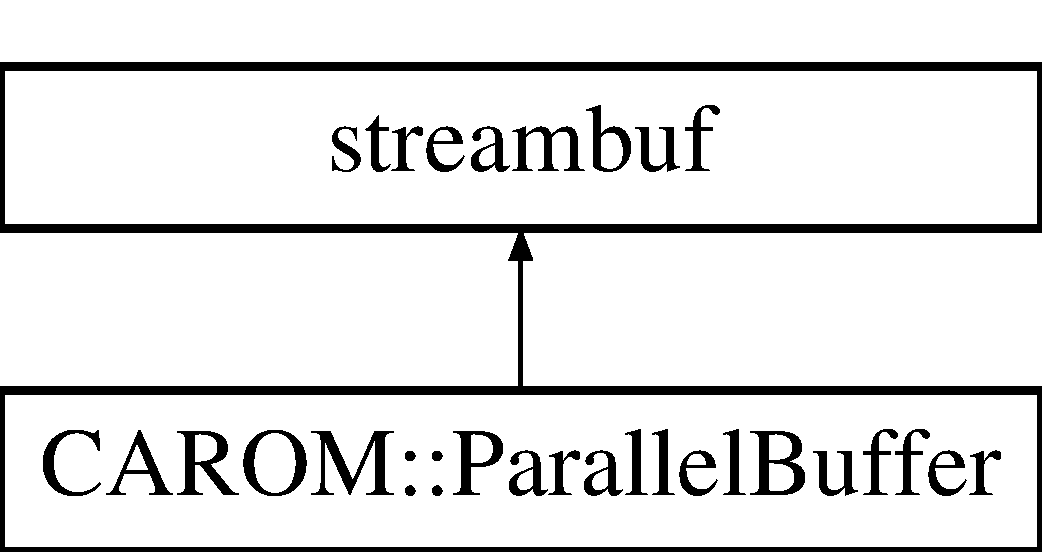
\includegraphics[height=2.000000cm]{class_c_a_r_o_m_1_1_parallel_buffer}
\end{center}
\end{figure}
\subsection*{Public Member Functions}
\begin{DoxyCompactItemize}
\item 
\hyperlink{class_c_a_r_o_m_1_1_parallel_buffer_ab2b7b484f4b3ca7fd5b94c0831a280d4}{Parallel\-Buffer} ()
\begin{DoxyCompactList}\small\item\em Default constructor. \end{DoxyCompactList}\item 
\hyperlink{class_c_a_r_o_m_1_1_parallel_buffer_a59d63b50bbf75f26af7540687a42a9d3}{$\sim$\-Parallel\-Buffer} ()
\begin{DoxyCompactList}\small\item\em Destructor. \end{DoxyCompactList}\item 
void \hyperlink{class_c_a_r_o_m_1_1_parallel_buffer_abd566a2c8afc78b3d1c97cb8c6aec460}{output\-String} (const std\-::string \&text)
\begin{DoxyCompactList}\small\item\em Write a text string to the output stream. \end{DoxyCompactList}\item 
void \hyperlink{class_c_a_r_o_m_1_1_parallel_buffer_a9be0cf7fefe904c01968a87160ce1c26}{output\-String} (const std\-::string \&text, int length)
\begin{DoxyCompactList}\small\item\em Write a text string of the specified length to the output file. \end{DoxyCompactList}\item 
int \hyperlink{class_c_a_r_o_m_1_1_parallel_buffer_a53f1cd6e167519b793e9bd830659f8c9}{sync} ()
\begin{DoxyCompactList}\small\item\em Synchronize the parallel buffer (called from streambuf). \end{DoxyCompactList}\item 
int \hyperlink{class_c_a_r_o_m_1_1_parallel_buffer_a17520235bc6ce13367a96179558d2419}{overflow} (int ch)
\begin{DoxyCompactList}\small\item\em Write an overflow character into the parallel buffer (called from streambuf). \end{DoxyCompactList}\end{DoxyCompactItemize}


\subsection{Detailed Description}
Class \hyperlink{class_c_a_r_o_m_1_1_parallel_buffer}{Parallel\-Buffer} is a simple I/\-O stream utility that intercepts output from an ostream and redirects the output as necessary for parallel I/\-O. This class defines a stream buffer class for an ostream class. 

\subsection{Constructor \& Destructor Documentation}
\hypertarget{class_c_a_r_o_m_1_1_parallel_buffer_ab2b7b484f4b3ca7fd5b94c0831a280d4}{\index{C\-A\-R\-O\-M\-::\-Parallel\-Buffer@{C\-A\-R\-O\-M\-::\-Parallel\-Buffer}!Parallel\-Buffer@{Parallel\-Buffer}}
\index{Parallel\-Buffer@{Parallel\-Buffer}!CAROM::ParallelBuffer@{C\-A\-R\-O\-M\-::\-Parallel\-Buffer}}
\subsubsection[{Parallel\-Buffer}]{\setlength{\rightskip}{0pt plus 5cm}C\-A\-R\-O\-M\-::\-Parallel\-Buffer\-::\-Parallel\-Buffer (
\begin{DoxyParamCaption}
{}
\end{DoxyParamCaption}
)}}\label{class_c_a_r_o_m_1_1_parallel_buffer_ab2b7b484f4b3ca7fd5b94c0831a280d4}


Default constructor. 

The object will require further initialization to set up the I/\-O streams and prefix string. \hypertarget{class_c_a_r_o_m_1_1_parallel_buffer_a59d63b50bbf75f26af7540687a42a9d3}{\index{C\-A\-R\-O\-M\-::\-Parallel\-Buffer@{C\-A\-R\-O\-M\-::\-Parallel\-Buffer}!$\sim$\-Parallel\-Buffer@{$\sim$\-Parallel\-Buffer}}
\index{$\sim$\-Parallel\-Buffer@{$\sim$\-Parallel\-Buffer}!CAROM::ParallelBuffer@{C\-A\-R\-O\-M\-::\-Parallel\-Buffer}}
\subsubsection[{$\sim$\-Parallel\-Buffer}]{\setlength{\rightskip}{0pt plus 5cm}C\-A\-R\-O\-M\-::\-Parallel\-Buffer\-::$\sim$\-Parallel\-Buffer (
\begin{DoxyParamCaption}
{}
\end{DoxyParamCaption}
)}}\label{class_c_a_r_o_m_1_1_parallel_buffer_a59d63b50bbf75f26af7540687a42a9d3}


Destructor. 

Simply deallocates any internal data buffers. It does not modify the output streams. 

\subsection{Member Function Documentation}
\hypertarget{class_c_a_r_o_m_1_1_parallel_buffer_abd566a2c8afc78b3d1c97cb8c6aec460}{\index{C\-A\-R\-O\-M\-::\-Parallel\-Buffer@{C\-A\-R\-O\-M\-::\-Parallel\-Buffer}!output\-String@{output\-String}}
\index{output\-String@{output\-String}!CAROM::ParallelBuffer@{C\-A\-R\-O\-M\-::\-Parallel\-Buffer}}
\subsubsection[{output\-String}]{\setlength{\rightskip}{0pt plus 5cm}void C\-A\-R\-O\-M\-::\-Parallel\-Buffer\-::output\-String (
\begin{DoxyParamCaption}
\item[{const std\-::string \&}]{text}
\end{DoxyParamCaption}
)\hspace{0.3cm}{\ttfamily [inline]}}}\label{class_c_a_r_o_m_1_1_parallel_buffer_abd566a2c8afc78b3d1c97cb8c6aec460}


Write a text string to the output stream. 

Note that the string is not actually written until an end-\/of-\/line is detected.


\begin{DoxyParams}[1]{Parameters}
\mbox{\tt in}  & {\em text} & The string to be written. \\
\hline
\end{DoxyParams}
\hypertarget{class_c_a_r_o_m_1_1_parallel_buffer_a9be0cf7fefe904c01968a87160ce1c26}{\index{C\-A\-R\-O\-M\-::\-Parallel\-Buffer@{C\-A\-R\-O\-M\-::\-Parallel\-Buffer}!output\-String@{output\-String}}
\index{output\-String@{output\-String}!CAROM::ParallelBuffer@{C\-A\-R\-O\-M\-::\-Parallel\-Buffer}}
\subsubsection[{output\-String}]{\setlength{\rightskip}{0pt plus 5cm}void C\-A\-R\-O\-M\-::\-Parallel\-Buffer\-::output\-String (
\begin{DoxyParamCaption}
\item[{const std\-::string \&}]{text, }
\item[{int}]{length}
\end{DoxyParamCaption}
)}}\label{class_c_a_r_o_m_1_1_parallel_buffer_a9be0cf7fefe904c01968a87160ce1c26}


Write a text string of the specified length to the output file. 

Note that the string is not actually written until an end-\/of-\/line is detected.


\begin{DoxyParams}[1]{Parameters}
\mbox{\tt in}  & {\em text} & The string to be written. \\
\hline
\mbox{\tt in}  & {\em length} & The length of the string. \\
\hline
\end{DoxyParams}
\hypertarget{class_c_a_r_o_m_1_1_parallel_buffer_a17520235bc6ce13367a96179558d2419}{\index{C\-A\-R\-O\-M\-::\-Parallel\-Buffer@{C\-A\-R\-O\-M\-::\-Parallel\-Buffer}!overflow@{overflow}}
\index{overflow@{overflow}!CAROM::ParallelBuffer@{C\-A\-R\-O\-M\-::\-Parallel\-Buffer}}
\subsubsection[{overflow}]{\setlength{\rightskip}{0pt plus 5cm}int C\-A\-R\-O\-M\-::\-Parallel\-Buffer\-::overflow (
\begin{DoxyParamCaption}
\item[{int}]{ch}
\end{DoxyParamCaption}
)}}\label{class_c_a_r_o_m_1_1_parallel_buffer_a17520235bc6ce13367a96179558d2419}


Write an overflow character into the parallel buffer (called from streambuf). 


\begin{DoxyParams}[1]{Parameters}
\mbox{\tt in}  & {\em ch} & The character to write.\\
\hline
\end{DoxyParams}
\begin{DoxyReturn}{Returns}
0 
\end{DoxyReturn}
\hypertarget{class_c_a_r_o_m_1_1_parallel_buffer_a53f1cd6e167519b793e9bd830659f8c9}{\index{C\-A\-R\-O\-M\-::\-Parallel\-Buffer@{C\-A\-R\-O\-M\-::\-Parallel\-Buffer}!sync@{sync}}
\index{sync@{sync}!CAROM::ParallelBuffer@{C\-A\-R\-O\-M\-::\-Parallel\-Buffer}}
\subsubsection[{sync}]{\setlength{\rightskip}{0pt plus 5cm}int C\-A\-R\-O\-M\-::\-Parallel\-Buffer\-::sync (
\begin{DoxyParamCaption}
{}
\end{DoxyParamCaption}
)}}\label{class_c_a_r_o_m_1_1_parallel_buffer_a53f1cd6e167519b793e9bd830659f8c9}


Synchronize the parallel buffer (called from streambuf). 

\begin{DoxyReturn}{Returns}
0 
\end{DoxyReturn}


The documentation for this class was generated from the following file\-:\begin{DoxyCompactItemize}
\item 
Parallel\-Buffer.\-h\end{DoxyCompactItemize}

\hypertarget{class_c_a_r_o_m_1_1_randomized_s_v_d}{\section{C\-A\-R\-O\-M\-:\-:Randomized\-S\-V\-D Class Reference}
\label{class_c_a_r_o_m_1_1_randomized_s_v_d}\index{C\-A\-R\-O\-M\-::\-Randomized\-S\-V\-D@{C\-A\-R\-O\-M\-::\-Randomized\-S\-V\-D}}
}


{\ttfamily \#include $<$Randomized\-S\-V\-D.\-h$>$}

Inheritance diagram for C\-A\-R\-O\-M\-:\-:Randomized\-S\-V\-D\-:\begin{figure}[H]
\begin{center}
\leavevmode
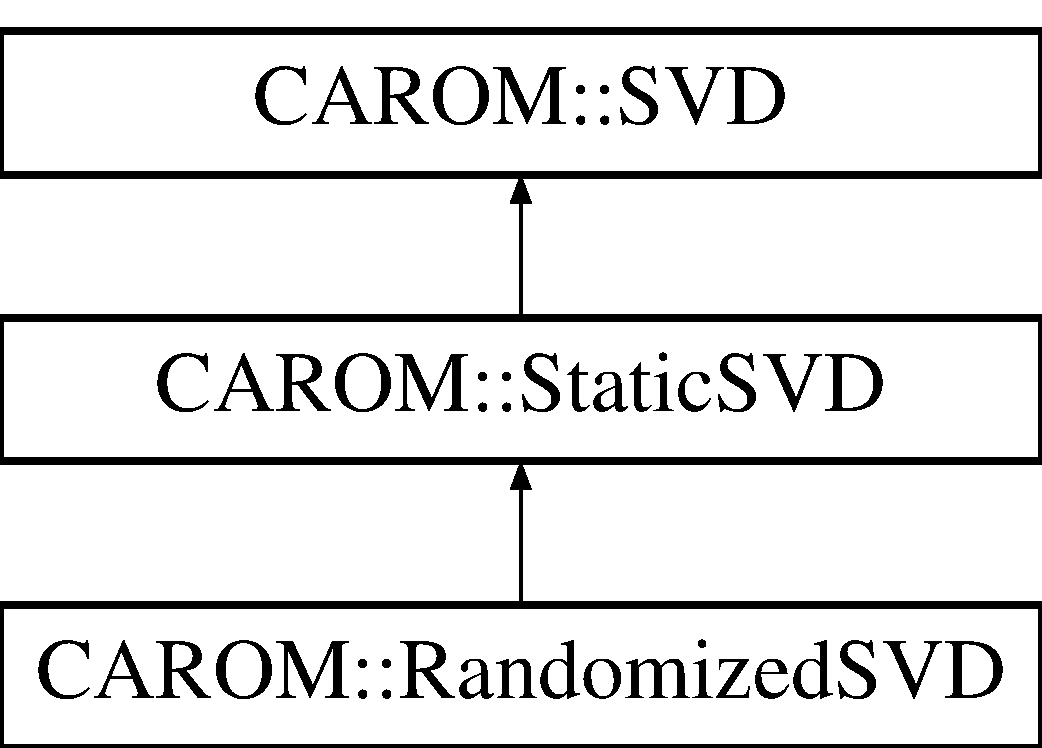
\includegraphics[height=3.000000cm]{class_c_a_r_o_m_1_1_randomized_s_v_d}
\end{center}
\end{figure}
\subsection*{Friends}
\begin{DoxyCompactItemize}
\item 
\hypertarget{class_c_a_r_o_m_1_1_randomized_s_v_d_a14677f178902af98cccb02b0058fd326}{class {\bfseries Basis\-Generator}}\label{class_c_a_r_o_m_1_1_randomized_s_v_d_a14677f178902af98cccb02b0058fd326}

\end{DoxyCompactItemize}
\subsection*{Additional Inherited Members}


\subsection{Detailed Description}
Class \hyperlink{class_c_a_r_o_m_1_1_randomized_s_v_d}{Randomized\-S\-V\-D} implements the Randomized \hyperlink{class_c_a_r_o_m_1_1_s_v_d}{S\-V\-D} algorithm introduced in \char`\"{}\-Finding Structure with Randomness\-: Probabilistic Algorithms for
   Constructing Approximate Matrix Decompositions\char`\"{} by N. Halko, P. G. Martinsson, and J. A. Tropp 

The documentation for this class was generated from the following file\-:\begin{DoxyCompactItemize}
\item 
Randomized\-S\-V\-D.\-h\end{DoxyCompactItemize}

\hypertarget{class_c_a_r_o_m_1_1_static_s_v_d}{\section{C\-A\-R\-O\-M\-:\-:Static\-S\-V\-D Class Reference}
\label{class_c_a_r_o_m_1_1_static_s_v_d}\index{C\-A\-R\-O\-M\-::\-Static\-S\-V\-D@{C\-A\-R\-O\-M\-::\-Static\-S\-V\-D}}
}


{\ttfamily \#include $<$Static\-S\-V\-D.\-h$>$}

Inheritance diagram for C\-A\-R\-O\-M\-:\-:Static\-S\-V\-D\-:\begin{figure}[H]
\begin{center}
\leavevmode
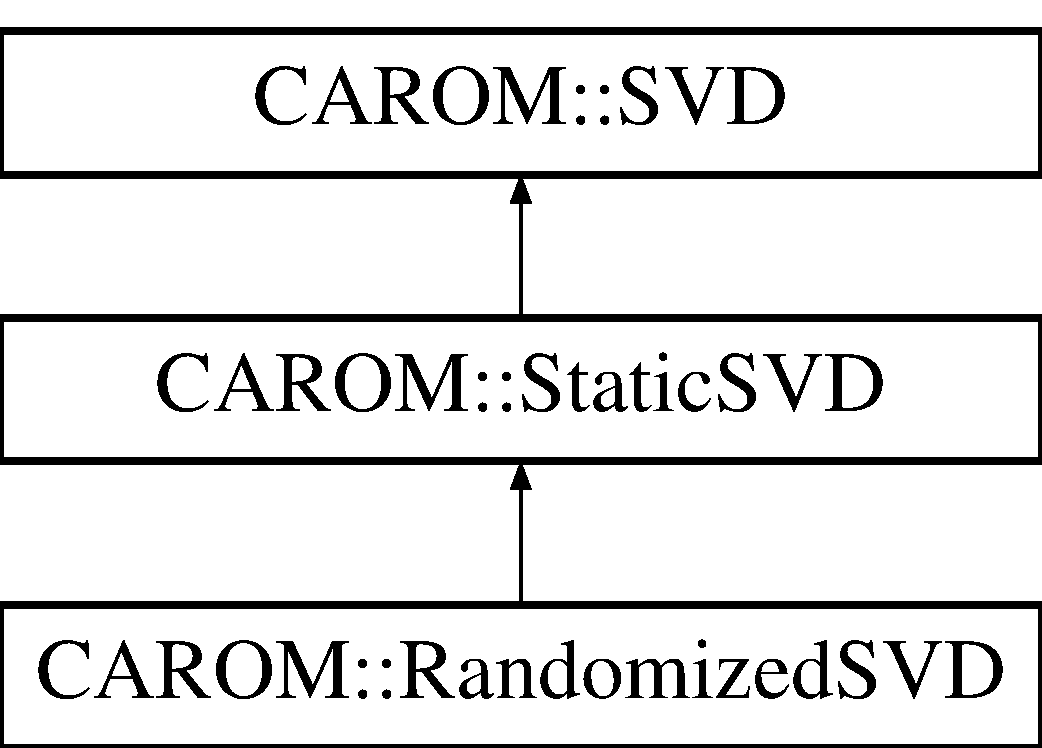
\includegraphics[height=3.000000cm]{class_c_a_r_o_m_1_1_static_s_v_d}
\end{center}
\end{figure}
\subsection*{Public Member Functions}
\begin{DoxyCompactItemize}
\item 
\hyperlink{class_c_a_r_o_m_1_1_static_s_v_d_a38fe9d5c3d8ef47f0e40353078015e7a}{$\sim$\-Static\-S\-V\-D} ()
\item 
virtual bool \hyperlink{class_c_a_r_o_m_1_1_static_s_v_d_a6776aa994a771b6b4a39a96a77f8e6c2}{take\-Sample} (double $\ast$u\-\_\-in, double time, bool add\-\_\-without\-\_\-increase=false)
\begin{DoxyCompactList}\small\item\em Collect the new sample, u\-\_\-in at the supplied time. \end{DoxyCompactList}\item 
virtual const \hyperlink{class_c_a_r_o_m_1_1_matrix}{Matrix} $\ast$ \hyperlink{class_c_a_r_o_m_1_1_static_s_v_d_aafd2a6fe2b2488fb24160d80013a7194}{get\-Spatial\-Basis} ()
\begin{DoxyCompactList}\small\item\em Returns the basis vectors for the current time interval as a \hyperlink{class_c_a_r_o_m_1_1_matrix}{Matrix}. \end{DoxyCompactList}\item 
virtual const \hyperlink{class_c_a_r_o_m_1_1_matrix}{Matrix} $\ast$ \hyperlink{class_c_a_r_o_m_1_1_static_s_v_d_a25750394f6513f0ae99dfd02f513b1da}{get\-Temporal\-Basis} ()
\begin{DoxyCompactList}\small\item\em Returns the temporal basis vectors for the current time interval as a \hyperlink{class_c_a_r_o_m_1_1_matrix}{Matrix}. \end{DoxyCompactList}\item 
virtual const \hyperlink{class_c_a_r_o_m_1_1_vector}{Vector} $\ast$ \hyperlink{class_c_a_r_o_m_1_1_static_s_v_d_abbb6aebb985310c464040746e597a4da}{get\-Singular\-Values} ()
\begin{DoxyCompactList}\small\item\em Returns the singular values for the current time interval. \end{DoxyCompactList}\item 
virtual const \hyperlink{class_c_a_r_o_m_1_1_matrix}{Matrix} $\ast$ \hyperlink{class_c_a_r_o_m_1_1_static_s_v_d_afd8e0bf6c2e53a39e47e7554eba3f8f0}{get\-Snapshot\-Matrix} ()
\begin{DoxyCompactList}\small\item\em Returns the snapshot matrix for the current time interval. \end{DoxyCompactList}\end{DoxyCompactItemize}
\subsection*{Protected Member Functions}
\begin{DoxyCompactItemize}
\item 
\hyperlink{class_c_a_r_o_m_1_1_static_s_v_d_a7db32fa4778422244a7b5230f9b7481f}{Static\-S\-V\-D} (\hyperlink{class_c_a_r_o_m_1_1_options}{Options} options)
\begin{DoxyCompactList}\small\item\em Constructor. \end{DoxyCompactList}\item 
\hypertarget{class_c_a_r_o_m_1_1_static_s_v_d_a84a3a716b20657be429866c873424e3c}{virtual void \hyperlink{class_c_a_r_o_m_1_1_static_s_v_d_a84a3a716b20657be429866c873424e3c}{compute\-S\-V\-D} ()}\label{class_c_a_r_o_m_1_1_static_s_v_d_a84a3a716b20657be429866c873424e3c}

\begin{DoxyCompactList}\small\item\em Gathers samples from all other processors to form complete sample of system and computes the \hyperlink{class_c_a_r_o_m_1_1_s_v_d}{S\-V\-D}. \end{DoxyCompactList}\item 
bool \hyperlink{class_c_a_r_o_m_1_1_static_s_v_d_a8c59671fcd305f798bc3c185b6595345}{this\-Interval\-Basis\-Current} ()
\begin{DoxyCompactList}\small\item\em Checks if the basis vectors for this time interval are up to date. \end{DoxyCompactList}\item 
\hypertarget{class_c_a_r_o_m_1_1_static_s_v_d_a4871175e1c83e6a3013595ffad89e248}{void \hyperlink{class_c_a_r_o_m_1_1_static_s_v_d_a4871175e1c83e6a3013595ffad89e248}{get\-\_\-global\-\_\-info} ()}\label{class_c_a_r_o_m_1_1_static_s_v_d_a4871175e1c83e6a3013595ffad89e248}

\begin{DoxyCompactList}\small\item\em Get the system's total row dimension and where my rows sit in the matrix. \end{DoxyCompactList}\item 
\hypertarget{class_c_a_r_o_m_1_1_static_s_v_d_a48c3bc32b0d15ad95fe9a9966581157a}{void \hyperlink{class_c_a_r_o_m_1_1_static_s_v_d_a48c3bc32b0d15ad95fe9a9966581157a}{delete\-\_\-samples} ()}\label{class_c_a_r_o_m_1_1_static_s_v_d_a48c3bc32b0d15ad95fe9a9966581157a}

\begin{DoxyCompactList}\small\item\em Delete the samples from Sca\-L\-A\-P\-A\-C\-K. \end{DoxyCompactList}\item 
\hypertarget{class_c_a_r_o_m_1_1_static_s_v_d_a4539c67bd0fc29dde6603173c6eaeffd}{void \hyperlink{class_c_a_r_o_m_1_1_static_s_v_d_a4539c67bd0fc29dde6603173c6eaeffd}{delete\-\_\-factorizer} ()}\label{class_c_a_r_o_m_1_1_static_s_v_d_a4539c67bd0fc29dde6603173c6eaeffd}

\begin{DoxyCompactList}\small\item\em Delete the factorizer from Sca\-L\-A\-P\-A\-C\-K. \end{DoxyCompactList}\item 
\hypertarget{class_c_a_r_o_m_1_1_static_s_v_d_a5dd0024af19c1c302b4b374a11b1bcd7}{void \hyperlink{class_c_a_r_o_m_1_1_static_s_v_d_a5dd0024af19c1c302b4b374a11b1bcd7}{broadcast\-\_\-sample} (const double $\ast$u\-\_\-in)}\label{class_c_a_r_o_m_1_1_static_s_v_d_a5dd0024af19c1c302b4b374a11b1bcd7}

\begin{DoxyCompactList}\small\item\em Broadcast the sample to all processors. \end{DoxyCompactList}\end{DoxyCompactItemize}
\subsection*{Protected Attributes}
\begin{DoxyCompactItemize}
\item 
\hypertarget{class_c_a_r_o_m_1_1_static_s_v_d_a9c41d5d0f382d40e30052faae9d8ed53}{std\-::unique\-\_\-ptr$<$ S\-L\-P\-K\-\_\-\-Matrix $>$ \hyperlink{class_c_a_r_o_m_1_1_static_s_v_d_a9c41d5d0f382d40e30052faae9d8ed53}{d\-\_\-samples}}\label{class_c_a_r_o_m_1_1_static_s_v_d_a9c41d5d0f382d40e30052faae9d8ed53}

\begin{DoxyCompactList}\small\item\em Current samples of the system. \end{DoxyCompactList}\item 
\hypertarget{class_c_a_r_o_m_1_1_static_s_v_d_ab190353592dfd9c6ba6ceb3853e5d3a7}{std\-::unique\-\_\-ptr$<$ S\-V\-D\-Manager $>$ \hyperlink{class_c_a_r_o_m_1_1_static_s_v_d_ab190353592dfd9c6ba6ceb3853e5d3a7}{d\-\_\-factorizer}}\label{class_c_a_r_o_m_1_1_static_s_v_d_ab190353592dfd9c6ba6ceb3853e5d3a7}

\begin{DoxyCompactList}\small\item\em Factorization manager object used to compute the \hyperlink{class_c_a_r_o_m_1_1_s_v_d}{S\-V\-D}. \end{DoxyCompactList}\item 
\hypertarget{class_c_a_r_o_m_1_1_static_s_v_d_a807ec34cff9fe5e62ae2f84cd8dad151}{bool \hyperlink{class_c_a_r_o_m_1_1_static_s_v_d_a807ec34cff9fe5e62ae2f84cd8dad151}{d\-\_\-this\-\_\-interval\-\_\-basis\-\_\-current}}\label{class_c_a_r_o_m_1_1_static_s_v_d_a807ec34cff9fe5e62ae2f84cd8dad151}

\begin{DoxyCompactList}\small\item\em Flag to indicate if the basis vectors for the current time interval are up to date. \end{DoxyCompactList}\item 
\hypertarget{class_c_a_r_o_m_1_1_static_s_v_d_a1454841fa7e3afaae10f52583ef4b8fe}{int \hyperlink{class_c_a_r_o_m_1_1_static_s_v_d_a1454841fa7e3afaae10f52583ef4b8fe}{d\-\_\-rank}}\label{class_c_a_r_o_m_1_1_static_s_v_d_a1454841fa7e3afaae10f52583ef4b8fe}

\begin{DoxyCompactList}\small\item\em The rank of the process this object belongs to. \end{DoxyCompactList}\item 
\hypertarget{class_c_a_r_o_m_1_1_static_s_v_d_ad3e3b35402a5ef9813dd9a0d403e2212}{int \hyperlink{class_c_a_r_o_m_1_1_static_s_v_d_ad3e3b35402a5ef9813dd9a0d403e2212}{d\-\_\-num\-\_\-procs}}\label{class_c_a_r_o_m_1_1_static_s_v_d_ad3e3b35402a5ef9813dd9a0d403e2212}

\begin{DoxyCompactList}\small\item\em The number of processors being run on. \end{DoxyCompactList}\item 
\hypertarget{class_c_a_r_o_m_1_1_static_s_v_d_a681f31b3a5c8e134346865e21d33f8e0}{std\-::vector$<$ int $>$ \hyperlink{class_c_a_r_o_m_1_1_static_s_v_d_a681f31b3a5c8e134346865e21d33f8e0}{d\-\_\-istarts}}\label{class_c_a_r_o_m_1_1_static_s_v_d_a681f31b3a5c8e134346865e21d33f8e0}

\begin{DoxyCompactList}\small\item\em The starting row (0-\/based) of the matrix that each process owns. Stored to avoid an M\-P\-I operation to get this operation every time we scatter a sample. \end{DoxyCompactList}\item 
\hypertarget{class_c_a_r_o_m_1_1_static_s_v_d_aee0dd1ce7f230cec30ca51b3206f5d3d}{std\-::vector$<$ int $>$ \hyperlink{class_c_a_r_o_m_1_1_static_s_v_d_aee0dd1ce7f230cec30ca51b3206f5d3d}{d\-\_\-dims}}\label{class_c_a_r_o_m_1_1_static_s_v_d_aee0dd1ce7f230cec30ca51b3206f5d3d}

\begin{DoxyCompactList}\small\item\em The number of rows that each process owns. Stored to avoid an M\-P\-I operation to get this operation every time we scatter a sample. \end{DoxyCompactList}\item 
\hypertarget{class_c_a_r_o_m_1_1_static_s_v_d_a73e6408bd26fba550ba23a7dee558dd0}{int \hyperlink{class_c_a_r_o_m_1_1_static_s_v_d_a73e6408bd26fba550ba23a7dee558dd0}{d\-\_\-total\-\_\-dim}}\label{class_c_a_r_o_m_1_1_static_s_v_d_a73e6408bd26fba550ba23a7dee558dd0}

\begin{DoxyCompactList}\small\item\em The total dimension of the system (row dimension) \end{DoxyCompactList}\item 
\hypertarget{class_c_a_r_o_m_1_1_static_s_v_d_a1d66d0c978bdb071e57e4c90fe0fbd0c}{int \hyperlink{class_c_a_r_o_m_1_1_static_s_v_d_a1d66d0c978bdb071e57e4c90fe0fbd0c}{d\-\_\-nprow}}\label{class_c_a_r_o_m_1_1_static_s_v_d_a1d66d0c978bdb071e57e4c90fe0fbd0c}

\begin{DoxyCompactList}\small\item\em The number of processor rows in the grid. \end{DoxyCompactList}\item 
\hypertarget{class_c_a_r_o_m_1_1_static_s_v_d_a3f8e127315710034a70c05f11a58198b}{int \hyperlink{class_c_a_r_o_m_1_1_static_s_v_d_a3f8e127315710034a70c05f11a58198b}{d\-\_\-npcol}}\label{class_c_a_r_o_m_1_1_static_s_v_d_a3f8e127315710034a70c05f11a58198b}

\begin{DoxyCompactList}\small\item\em The number of processor columns in the grid. \end{DoxyCompactList}\item 
\hypertarget{class_c_a_r_o_m_1_1_static_s_v_d_ab9136905dc7a77975aa22baf5b26cebf}{int \hyperlink{class_c_a_r_o_m_1_1_static_s_v_d_ab9136905dc7a77975aa22baf5b26cebf}{d\-\_\-blocksize}}\label{class_c_a_r_o_m_1_1_static_s_v_d_ab9136905dc7a77975aa22baf5b26cebf}

\begin{DoxyCompactList}\small\item\em The block size used internally for computing the \hyperlink{class_c_a_r_o_m_1_1_s_v_d}{S\-V\-D}. \end{DoxyCompactList}\item 
\hypertarget{class_c_a_r_o_m_1_1_static_s_v_d_a8ccff71fcfbf639a2f38a1e438f520dd}{int \hyperlink{class_c_a_r_o_m_1_1_static_s_v_d_a8ccff71fcfbf639a2f38a1e438f520dd}{d\-\_\-max\-\_\-basis\-\_\-dimension}}\label{class_c_a_r_o_m_1_1_static_s_v_d_a8ccff71fcfbf639a2f38a1e438f520dd}

\begin{DoxyCompactList}\small\item\em The max number of basis vectors to return. \end{DoxyCompactList}\item 
\hypertarget{class_c_a_r_o_m_1_1_static_s_v_d_a02d8eb7feaad508faa2abba9e1de6a4f}{double \hyperlink{class_c_a_r_o_m_1_1_static_s_v_d_a02d8eb7feaad508faa2abba9e1de6a4f}{d\-\_\-singular\-\_\-value\-\_\-tol}}\label{class_c_a_r_o_m_1_1_static_s_v_d_a02d8eb7feaad508faa2abba9e1de6a4f}

\begin{DoxyCompactList}\small\item\em The tolerance for singular values below which to drop vectors. \end{DoxyCompactList}\end{DoxyCompactItemize}
\subsection*{Friends}
\begin{DoxyCompactItemize}
\item 
\hypertarget{class_c_a_r_o_m_1_1_static_s_v_d_a14677f178902af98cccb02b0058fd326}{class {\bfseries Basis\-Generator}}\label{class_c_a_r_o_m_1_1_static_s_v_d_a14677f178902af98cccb02b0058fd326}

\end{DoxyCompactItemize}


\subsection{Detailed Description}
\hyperlink{class_c_a_r_o_m_1_1_static_s_v_d}{Static\-S\-V\-D} implements the interface of class \hyperlink{class_c_a_r_o_m_1_1_s_v_d}{S\-V\-D} for the static \hyperlink{class_c_a_r_o_m_1_1_s_v_d}{S\-V\-D} algorithm. This algorithm is not scalable and is intended primarily as a sanity check of the incremental \hyperlink{class_c_a_r_o_m_1_1_s_v_d}{S\-V\-D} algorithm. 

\subsection{Constructor \& Destructor Documentation}
\hypertarget{class_c_a_r_o_m_1_1_static_s_v_d_a38fe9d5c3d8ef47f0e40353078015e7a}{\index{C\-A\-R\-O\-M\-::\-Static\-S\-V\-D@{C\-A\-R\-O\-M\-::\-Static\-S\-V\-D}!$\sim$\-Static\-S\-V\-D@{$\sim$\-Static\-S\-V\-D}}
\index{$\sim$\-Static\-S\-V\-D@{$\sim$\-Static\-S\-V\-D}!CAROM::StaticSVD@{C\-A\-R\-O\-M\-::\-Static\-S\-V\-D}}
\subsubsection[{$\sim$\-Static\-S\-V\-D}]{\setlength{\rightskip}{0pt plus 5cm}C\-A\-R\-O\-M\-::\-Static\-S\-V\-D\-::$\sim$\-Static\-S\-V\-D (
\begin{DoxyParamCaption}
{}
\end{DoxyParamCaption}
)}}\label{class_c_a_r_o_m_1_1_static_s_v_d_a38fe9d5c3d8ef47f0e40353078015e7a}
Destructor. \hypertarget{class_c_a_r_o_m_1_1_static_s_v_d_a7db32fa4778422244a7b5230f9b7481f}{\index{C\-A\-R\-O\-M\-::\-Static\-S\-V\-D@{C\-A\-R\-O\-M\-::\-Static\-S\-V\-D}!Static\-S\-V\-D@{Static\-S\-V\-D}}
\index{Static\-S\-V\-D@{Static\-S\-V\-D}!CAROM::StaticSVD@{C\-A\-R\-O\-M\-::\-Static\-S\-V\-D}}
\subsubsection[{Static\-S\-V\-D}]{\setlength{\rightskip}{0pt plus 5cm}C\-A\-R\-O\-M\-::\-Static\-S\-V\-D\-::\-Static\-S\-V\-D (
\begin{DoxyParamCaption}
\item[{{\bf Options}}]{options}
\end{DoxyParamCaption}
)\hspace{0.3cm}{\ttfamily [protected]}}}\label{class_c_a_r_o_m_1_1_static_s_v_d_a7db32fa4778422244a7b5230f9b7481f}


Constructor. 


\begin{DoxyParams}[1]{Parameters}
\mbox{\tt in}  & {\em options} & The struct containing the options for this \hyperlink{class_c_a_r_o_m_1_1_s_v_d}{S\-V\-D} implementation. \\
\hline
\end{DoxyParams}
\begin{DoxySeeAlso}{See Also}
\hyperlink{class_c_a_r_o_m_1_1_options}{Options} 
\end{DoxySeeAlso}


\subsection{Member Function Documentation}
\hypertarget{class_c_a_r_o_m_1_1_static_s_v_d_abbb6aebb985310c464040746e597a4da}{\index{C\-A\-R\-O\-M\-::\-Static\-S\-V\-D@{C\-A\-R\-O\-M\-::\-Static\-S\-V\-D}!get\-Singular\-Values@{get\-Singular\-Values}}
\index{get\-Singular\-Values@{get\-Singular\-Values}!CAROM::StaticSVD@{C\-A\-R\-O\-M\-::\-Static\-S\-V\-D}}
\subsubsection[{get\-Singular\-Values}]{\setlength{\rightskip}{0pt plus 5cm}virtual const {\bf Vector}$\ast$ C\-A\-R\-O\-M\-::\-Static\-S\-V\-D\-::get\-Singular\-Values (
\begin{DoxyParamCaption}
{}
\end{DoxyParamCaption}
)\hspace{0.3cm}{\ttfamily [virtual]}}}\label{class_c_a_r_o_m_1_1_static_s_v_d_abbb6aebb985310c464040746e597a4da}


Returns the singular values for the current time interval. 

\begin{DoxyPostcond}{Postcondition}
\hyperlink{class_c_a_r_o_m_1_1_static_s_v_d_a8c59671fcd305f798bc3c185b6595345}{this\-Interval\-Basis\-Current()}
\end{DoxyPostcond}
\begin{DoxyReturn}{Returns}
The singular values for the current time interval. 
\end{DoxyReturn}


Implements \hyperlink{class_c_a_r_o_m_1_1_s_v_d_ab9bbaa07ffc11ef329be712669a6c95b}{C\-A\-R\-O\-M\-::\-S\-V\-D}.

\hypertarget{class_c_a_r_o_m_1_1_static_s_v_d_afd8e0bf6c2e53a39e47e7554eba3f8f0}{\index{C\-A\-R\-O\-M\-::\-Static\-S\-V\-D@{C\-A\-R\-O\-M\-::\-Static\-S\-V\-D}!get\-Snapshot\-Matrix@{get\-Snapshot\-Matrix}}
\index{get\-Snapshot\-Matrix@{get\-Snapshot\-Matrix}!CAROM::StaticSVD@{C\-A\-R\-O\-M\-::\-Static\-S\-V\-D}}
\subsubsection[{get\-Snapshot\-Matrix}]{\setlength{\rightskip}{0pt plus 5cm}virtual const {\bf Matrix}$\ast$ C\-A\-R\-O\-M\-::\-Static\-S\-V\-D\-::get\-Snapshot\-Matrix (
\begin{DoxyParamCaption}
{}
\end{DoxyParamCaption}
)\hspace{0.3cm}{\ttfamily [virtual]}}}\label{class_c_a_r_o_m_1_1_static_s_v_d_afd8e0bf6c2e53a39e47e7554eba3f8f0}


Returns the snapshot matrix for the current time interval. 

\begin{DoxyReturn}{Returns}
The snapshot matrix for the current time interval. 
\end{DoxyReturn}


Implements \hyperlink{class_c_a_r_o_m_1_1_s_v_d_a96b482e76d8c8f7278008af4a0bebf85}{C\-A\-R\-O\-M\-::\-S\-V\-D}.

\hypertarget{class_c_a_r_o_m_1_1_static_s_v_d_aafd2a6fe2b2488fb24160d80013a7194}{\index{C\-A\-R\-O\-M\-::\-Static\-S\-V\-D@{C\-A\-R\-O\-M\-::\-Static\-S\-V\-D}!get\-Spatial\-Basis@{get\-Spatial\-Basis}}
\index{get\-Spatial\-Basis@{get\-Spatial\-Basis}!CAROM::StaticSVD@{C\-A\-R\-O\-M\-::\-Static\-S\-V\-D}}
\subsubsection[{get\-Spatial\-Basis}]{\setlength{\rightskip}{0pt plus 5cm}virtual const {\bf Matrix}$\ast$ C\-A\-R\-O\-M\-::\-Static\-S\-V\-D\-::get\-Spatial\-Basis (
\begin{DoxyParamCaption}
{}
\end{DoxyParamCaption}
)\hspace{0.3cm}{\ttfamily [virtual]}}}\label{class_c_a_r_o_m_1_1_static_s_v_d_aafd2a6fe2b2488fb24160d80013a7194}


Returns the basis vectors for the current time interval as a \hyperlink{class_c_a_r_o_m_1_1_matrix}{Matrix}. 

\begin{DoxyPostcond}{Postcondition}
\hyperlink{class_c_a_r_o_m_1_1_static_s_v_d_a8c59671fcd305f798bc3c185b6595345}{this\-Interval\-Basis\-Current()}
\end{DoxyPostcond}
\begin{DoxyReturn}{Returns}
The basis vectors for the current time interval. 
\end{DoxyReturn}


Implements \hyperlink{class_c_a_r_o_m_1_1_s_v_d_ab152d85dfb91958d2265dd54046752dc}{C\-A\-R\-O\-M\-::\-S\-V\-D}.

\hypertarget{class_c_a_r_o_m_1_1_static_s_v_d_a25750394f6513f0ae99dfd02f513b1da}{\index{C\-A\-R\-O\-M\-::\-Static\-S\-V\-D@{C\-A\-R\-O\-M\-::\-Static\-S\-V\-D}!get\-Temporal\-Basis@{get\-Temporal\-Basis}}
\index{get\-Temporal\-Basis@{get\-Temporal\-Basis}!CAROM::StaticSVD@{C\-A\-R\-O\-M\-::\-Static\-S\-V\-D}}
\subsubsection[{get\-Temporal\-Basis}]{\setlength{\rightskip}{0pt plus 5cm}virtual const {\bf Matrix}$\ast$ C\-A\-R\-O\-M\-::\-Static\-S\-V\-D\-::get\-Temporal\-Basis (
\begin{DoxyParamCaption}
{}
\end{DoxyParamCaption}
)\hspace{0.3cm}{\ttfamily [virtual]}}}\label{class_c_a_r_o_m_1_1_static_s_v_d_a25750394f6513f0ae99dfd02f513b1da}


Returns the temporal basis vectors for the current time interval as a \hyperlink{class_c_a_r_o_m_1_1_matrix}{Matrix}. 

\begin{DoxyPostcond}{Postcondition}
\hyperlink{class_c_a_r_o_m_1_1_static_s_v_d_a8c59671fcd305f798bc3c185b6595345}{this\-Interval\-Basis\-Current()}
\end{DoxyPostcond}
\begin{DoxyReturn}{Returns}
The temporal basis vectors for the current time interval. 
\end{DoxyReturn}


Implements \hyperlink{class_c_a_r_o_m_1_1_s_v_d_a42820d67808cad0b5cc2af1590b98ff9}{C\-A\-R\-O\-M\-::\-S\-V\-D}.

\hypertarget{class_c_a_r_o_m_1_1_static_s_v_d_a6776aa994a771b6b4a39a96a77f8e6c2}{\index{C\-A\-R\-O\-M\-::\-Static\-S\-V\-D@{C\-A\-R\-O\-M\-::\-Static\-S\-V\-D}!take\-Sample@{take\-Sample}}
\index{take\-Sample@{take\-Sample}!CAROM::StaticSVD@{C\-A\-R\-O\-M\-::\-Static\-S\-V\-D}}
\subsubsection[{take\-Sample}]{\setlength{\rightskip}{0pt plus 5cm}virtual bool C\-A\-R\-O\-M\-::\-Static\-S\-V\-D\-::take\-Sample (
\begin{DoxyParamCaption}
\item[{double $\ast$}]{u\-\_\-in, }
\item[{double}]{time, }
\item[{bool}]{add\-\_\-without\-\_\-increase = {\ttfamily false}}
\end{DoxyParamCaption}
)\hspace{0.3cm}{\ttfamily [virtual]}}}\label{class_c_a_r_o_m_1_1_static_s_v_d_a6776aa994a771b6b4a39a96a77f8e6c2}


Collect the new sample, u\-\_\-in at the supplied time. 

\begin{DoxyPrecond}{Precondition}
u\-\_\-in != 0 

time $>$= 0.\-0
\end{DoxyPrecond}

\begin{DoxyParams}[1]{Parameters}
\mbox{\tt in}  & {\em u\-\_\-in} & The new sample. \\
\hline
\mbox{\tt in}  & {\em time} & The simulation time of the new sample. \\
\hline
\mbox{\tt in}  & {\em add\-\_\-without\-\_\-increase} & If true, then add\-Linearly\-Dependent will be invoked\\
\hline
\end{DoxyParams}
\begin{DoxyReturn}{Returns}
True if the sampling was successful. 
\end{DoxyReturn}


Implements \hyperlink{class_c_a_r_o_m_1_1_s_v_d_a5ed8a558690b130c49c2e923cc625769}{C\-A\-R\-O\-M\-::\-S\-V\-D}.

\hypertarget{class_c_a_r_o_m_1_1_static_s_v_d_a8c59671fcd305f798bc3c185b6595345}{\index{C\-A\-R\-O\-M\-::\-Static\-S\-V\-D@{C\-A\-R\-O\-M\-::\-Static\-S\-V\-D}!this\-Interval\-Basis\-Current@{this\-Interval\-Basis\-Current}}
\index{this\-Interval\-Basis\-Current@{this\-Interval\-Basis\-Current}!CAROM::StaticSVD@{C\-A\-R\-O\-M\-::\-Static\-S\-V\-D}}
\subsubsection[{this\-Interval\-Basis\-Current}]{\setlength{\rightskip}{0pt plus 5cm}bool C\-A\-R\-O\-M\-::\-Static\-S\-V\-D\-::this\-Interval\-Basis\-Current (
\begin{DoxyParamCaption}
{}
\end{DoxyParamCaption}
)\hspace{0.3cm}{\ttfamily [inline]}, {\ttfamily [protected]}}}\label{class_c_a_r_o_m_1_1_static_s_v_d_a8c59671fcd305f798bc3c185b6595345}


Checks if the basis vectors for this time interval are up to date. 

\begin{DoxyReturn}{Returns}
True if the basis vectors for this time interval are up to date. 
\end{DoxyReturn}


The documentation for this class was generated from the following file\-:\begin{DoxyCompactItemize}
\item 
Static\-S\-V\-D.\-h\end{DoxyCompactItemize}

\hypertarget{class_c_a_r_o_m_1_1_s_v_d}{\section{C\-A\-R\-O\-M\-:\-:S\-V\-D Class Reference}
\label{class_c_a_r_o_m_1_1_s_v_d}\index{C\-A\-R\-O\-M\-::\-S\-V\-D@{C\-A\-R\-O\-M\-::\-S\-V\-D}}
}


{\ttfamily \#include $<$S\-V\-D.\-h$>$}

Inheritance diagram for C\-A\-R\-O\-M\-:\-:S\-V\-D\-:\begin{figure}[H]
\begin{center}
\leavevmode
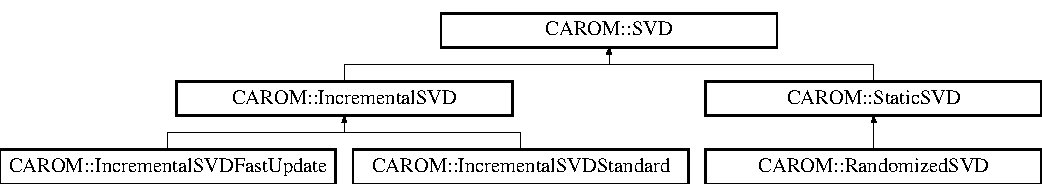
\includegraphics[height=2.466960cm]{class_c_a_r_o_m_1_1_s_v_d}
\end{center}
\end{figure}
\subsection*{Public Member Functions}
\begin{DoxyCompactItemize}
\item 
\hyperlink{class_c_a_r_o_m_1_1_s_v_d_a20c7b447885f81e763067da0685d04a4}{S\-V\-D} (\hyperlink{class_c_a_r_o_m_1_1_options}{Options} options)
\begin{DoxyCompactList}\small\item\em Constructor. \end{DoxyCompactList}\item 
\hyperlink{class_c_a_r_o_m_1_1_s_v_d_a4939973d4f9d812c74f6e749d91cc473}{$\sim$\-S\-V\-D} ()
\item 
virtual bool \hyperlink{class_c_a_r_o_m_1_1_s_v_d_a5ed8a558690b130c49c2e923cc625769}{take\-Sample} (double $\ast$u\-\_\-in, double time, bool add\-\_\-without\-\_\-increase)=0
\begin{DoxyCompactList}\small\item\em Collect the new sample, u\-\_\-in at supplied time. \end{DoxyCompactList}\item 
int \hyperlink{class_c_a_r_o_m_1_1_s_v_d_a66e6ad89757a715b8f5d6e01c205feb5}{get\-Dim} () const 
\begin{DoxyCompactList}\small\item\em Returns the dimension of the system on this processor. \end{DoxyCompactList}\item 
virtual const \hyperlink{class_c_a_r_o_m_1_1_matrix}{Matrix} $\ast$ \hyperlink{class_c_a_r_o_m_1_1_s_v_d_ab152d85dfb91958d2265dd54046752dc}{get\-Spatial\-Basis} ()=0
\begin{DoxyCompactList}\small\item\em Returns the basis vectors for the current time interval. \end{DoxyCompactList}\item 
virtual const \hyperlink{class_c_a_r_o_m_1_1_matrix}{Matrix} $\ast$ \hyperlink{class_c_a_r_o_m_1_1_s_v_d_a42820d67808cad0b5cc2af1590b98ff9}{get\-Temporal\-Basis} ()=0
\begin{DoxyCompactList}\small\item\em Returns the temporal basis vectors for the current time interval. \end{DoxyCompactList}\item 
virtual const \hyperlink{class_c_a_r_o_m_1_1_vector}{Vector} $\ast$ \hyperlink{class_c_a_r_o_m_1_1_s_v_d_ab9bbaa07ffc11ef329be712669a6c95b}{get\-Singular\-Values} ()=0
\begin{DoxyCompactList}\small\item\em Returns the singular values for the current time interval. \end{DoxyCompactList}\item 
virtual const \hyperlink{class_c_a_r_o_m_1_1_matrix}{Matrix} $\ast$ \hyperlink{class_c_a_r_o_m_1_1_s_v_d_a96b482e76d8c8f7278008af4a0bebf85}{get\-Snapshot\-Matrix} ()=0
\begin{DoxyCompactList}\small\item\em Returns the singular values for the current time interval. \end{DoxyCompactList}\item 
int \hyperlink{class_c_a_r_o_m_1_1_s_v_d_a4f9403bd1c9720a5515601162fc4923d}{get\-Num\-Basis\-Time\-Intervals} () const 
\begin{DoxyCompactList}\small\item\em Returns the number of time intervals on which different sets of basis vectors are defined. \end{DoxyCompactList}\item 
double \hyperlink{class_c_a_r_o_m_1_1_s_v_d_a671897e97a4135de6c3b03c49fd7fa91}{get\-Basis\-Interval\-Start\-Time} (int which\-\_\-interval) const 
\begin{DoxyCompactList}\small\item\em Returns the start time for the requested time interval. \end{DoxyCompactList}\item 
bool \hyperlink{class_c_a_r_o_m_1_1_s_v_d_a5eef5eb6cefc3feb64eaebe9fa1ac5a6}{is\-New\-Time\-Interval} () const 
\begin{DoxyCompactList}\small\item\em Returns true if the next sample will result in a new time interval. \end{DoxyCompactList}\item 
\hypertarget{class_c_a_r_o_m_1_1_s_v_d_a447e456c110129eef1565023065dc87d}{void \hyperlink{class_c_a_r_o_m_1_1_s_v_d_a447e456c110129eef1565023065dc87d}{increase\-Time\-Interval} ()}\label{class_c_a_r_o_m_1_1_s_v_d_a447e456c110129eef1565023065dc87d}

\begin{DoxyCompactList}\small\item\em Increase the number of time intervals by one. \end{DoxyCompactList}\item 
\hypertarget{class_c_a_r_o_m_1_1_s_v_d_a899aa5ebfaf2e10e3d2eeae179f23cc4}{int \hyperlink{class_c_a_r_o_m_1_1_s_v_d_a899aa5ebfaf2e10e3d2eeae179f23cc4}{get\-Num\-Samples} () const }\label{class_c_a_r_o_m_1_1_s_v_d_a899aa5ebfaf2e10e3d2eeae179f23cc4}

\begin{DoxyCompactList}\small\item\em Get the number of samples taken. \end{DoxyCompactList}\end{DoxyCompactItemize}
\subsection*{Protected Attributes}
\begin{DoxyCompactItemize}
\item 
\hypertarget{class_c_a_r_o_m_1_1_s_v_d_a1d34488c53c5699e51a5cef65a6caa9f}{int \hyperlink{class_c_a_r_o_m_1_1_s_v_d_a1d34488c53c5699e51a5cef65a6caa9f}{d\-\_\-dim}}\label{class_c_a_r_o_m_1_1_s_v_d_a1d34488c53c5699e51a5cef65a6caa9f}

\begin{DoxyCompactList}\small\item\em Dimension of the system. \end{DoxyCompactList}\item 
\hypertarget{class_c_a_r_o_m_1_1_s_v_d_a8ab3384bad0f105ccafeaca9015a96ee}{int \hyperlink{class_c_a_r_o_m_1_1_s_v_d_a8ab3384bad0f105ccafeaca9015a96ee}{d\-\_\-num\-\_\-samples}}\label{class_c_a_r_o_m_1_1_s_v_d_a8ab3384bad0f105ccafeaca9015a96ee}

\begin{DoxyCompactList}\small\item\em Number of samples stored for the current time interval. \end{DoxyCompactList}\item 
\hypertarget{class_c_a_r_o_m_1_1_s_v_d_a2336df07a9c7a9ae7d9ba070f7f8635a}{int \hyperlink{class_c_a_r_o_m_1_1_s_v_d_a2336df07a9c7a9ae7d9ba070f7f8635a}{d\-\_\-num\-\_\-rows\-\_\-of\-\_\-\-W}}\label{class_c_a_r_o_m_1_1_s_v_d_a2336df07a9c7a9ae7d9ba070f7f8635a}

\begin{DoxyCompactList}\small\item\em Number of rows in right singular matrix. \end{DoxyCompactList}\item 
\hypertarget{class_c_a_r_o_m_1_1_s_v_d_a51f01271f0c3bd30eb34bd50fbbcf23d}{const int \hyperlink{class_c_a_r_o_m_1_1_s_v_d_a51f01271f0c3bd30eb34bd50fbbcf23d}{d\-\_\-samples\-\_\-per\-\_\-time\-\_\-interval}}\label{class_c_a_r_o_m_1_1_s_v_d_a51f01271f0c3bd30eb34bd50fbbcf23d}

\begin{DoxyCompactList}\small\item\em The maximum number of samples to be collected for a time interval. \end{DoxyCompactList}\item 
\hypertarget{class_c_a_r_o_m_1_1_s_v_d_a102150ef1b4d72af0c43f1204a9b668a}{const int \hyperlink{class_c_a_r_o_m_1_1_s_v_d_a102150ef1b4d72af0c43f1204a9b668a}{d\-\_\-max\-\_\-time\-\_\-intervals}}\label{class_c_a_r_o_m_1_1_s_v_d_a102150ef1b4d72af0c43f1204a9b668a}

\begin{DoxyCompactList}\small\item\em The maximum number of time intervals. \end{DoxyCompactList}\item 
\hyperlink{class_c_a_r_o_m_1_1_matrix}{Matrix} $\ast$ \hyperlink{class_c_a_r_o_m_1_1_s_v_d_a01470350e59cca179cf019c194cb2fef}{d\-\_\-basis}
\begin{DoxyCompactList}\small\item\em The globalized basis vectors for the current time interval. \end{DoxyCompactList}\item 
\hyperlink{class_c_a_r_o_m_1_1_matrix}{Matrix} $\ast$ \hyperlink{class_c_a_r_o_m_1_1_s_v_d_a49f5c427062049cea8a815afbec966fe}{d\-\_\-basis\-\_\-right}
\begin{DoxyCompactList}\small\item\em The globalized right basis vectors for the current time interval. \end{DoxyCompactList}\item 
\hyperlink{class_c_a_r_o_m_1_1_matrix}{Matrix} $\ast$ \hyperlink{class_c_a_r_o_m_1_1_s_v_d_a8b9b2af990f5ced830dc37826a256491}{d\-\_\-\-U}
\begin{DoxyCompactList}\small\item\em The matrix U which is large. \end{DoxyCompactList}\item 
\hyperlink{class_c_a_r_o_m_1_1_matrix}{Matrix} $\ast$ \hyperlink{class_c_a_r_o_m_1_1_s_v_d_adb215548e00558097e34d4afad15035b}{d\-\_\-\-W}
\begin{DoxyCompactList}\small\item\em The matrix U which is large. \end{DoxyCompactList}\item 
\hyperlink{class_c_a_r_o_m_1_1_vector}{Vector} $\ast$ \hyperlink{class_c_a_r_o_m_1_1_s_v_d_a7e09dc0fc7a80f3718ba9da22406c4cb}{d\-\_\-\-S}
\begin{DoxyCompactList}\small\item\em The vector S which is small. \end{DoxyCompactList}\item 
\hyperlink{class_c_a_r_o_m_1_1_matrix}{Matrix} $\ast$ \hyperlink{class_c_a_r_o_m_1_1_s_v_d_a1a38d353f58b9d825ff23197a3a1a879}{d\-\_\-snapshots}
\begin{DoxyCompactList}\small\item\em The globalized snapshot vectors for the current time interval. \end{DoxyCompactList}\item 
\hypertarget{class_c_a_r_o_m_1_1_s_v_d_aeb7b11d0eaf47d84e38f15b3f285a579}{std\-::vector$<$ double $>$ \hyperlink{class_c_a_r_o_m_1_1_s_v_d_aeb7b11d0eaf47d84e38f15b3f285a579}{d\-\_\-time\-\_\-interval\-\_\-start\-\_\-times}}\label{class_c_a_r_o_m_1_1_s_v_d_aeb7b11d0eaf47d84e38f15b3f285a579}

\begin{DoxyCompactList}\small\item\em The simulation time at which each time interval starts. \end{DoxyCompactList}\item 
\hypertarget{class_c_a_r_o_m_1_1_s_v_d_a93d045f19df5eee0cb731e56a5b9926d}{bool \hyperlink{class_c_a_r_o_m_1_1_s_v_d_a93d045f19df5eee0cb731e56a5b9926d}{d\-\_\-debug\-\_\-algorithm}}\label{class_c_a_r_o_m_1_1_s_v_d_a93d045f19df5eee0cb731e56a5b9926d}

\begin{DoxyCompactList}\small\item\em Flag to indicate if results of algorithm should be printed for debugging purposes. \end{DoxyCompactList}\end{DoxyCompactItemize}


\subsection{Detailed Description}
Class \hyperlink{class_c_a_r_o_m_1_1_s_v_d}{S\-V\-D} defines the interface to the generic \hyperlink{class_c_a_r_o_m_1_1_s_v_d}{S\-V\-D} algorithm. The A\-P\-I is intentionally small. One may collect the samples, compute the \hyperlink{class_c_a_r_o_m_1_1_s_v_d}{S\-V\-D}, and get the dimension of the system. 

\subsection{Constructor \& Destructor Documentation}
\hypertarget{class_c_a_r_o_m_1_1_s_v_d_a20c7b447885f81e763067da0685d04a4}{\index{C\-A\-R\-O\-M\-::\-S\-V\-D@{C\-A\-R\-O\-M\-::\-S\-V\-D}!S\-V\-D@{S\-V\-D}}
\index{S\-V\-D@{S\-V\-D}!CAROM::SVD@{C\-A\-R\-O\-M\-::\-S\-V\-D}}
\subsubsection[{S\-V\-D}]{\setlength{\rightskip}{0pt plus 5cm}C\-A\-R\-O\-M\-::\-S\-V\-D\-::\-S\-V\-D (
\begin{DoxyParamCaption}
\item[{{\bf Options}}]{options}
\end{DoxyParamCaption}
)}}\label{class_c_a_r_o_m_1_1_s_v_d_a20c7b447885f81e763067da0685d04a4}


Constructor. 


\begin{DoxyParams}[1]{Parameters}
\mbox{\tt in}  & {\em options} & The struct containing the options for this abstract \hyperlink{class_c_a_r_o_m_1_1_s_v_d}{S\-V\-D} class. \\
\hline
\end{DoxyParams}
\begin{DoxySeeAlso}{See Also}
\hyperlink{class_c_a_r_o_m_1_1_options}{Options} 
\end{DoxySeeAlso}
\hypertarget{class_c_a_r_o_m_1_1_s_v_d_a4939973d4f9d812c74f6e749d91cc473}{\index{C\-A\-R\-O\-M\-::\-S\-V\-D@{C\-A\-R\-O\-M\-::\-S\-V\-D}!$\sim$\-S\-V\-D@{$\sim$\-S\-V\-D}}
\index{$\sim$\-S\-V\-D@{$\sim$\-S\-V\-D}!CAROM::SVD@{C\-A\-R\-O\-M\-::\-S\-V\-D}}
\subsubsection[{$\sim$\-S\-V\-D}]{\setlength{\rightskip}{0pt plus 5cm}C\-A\-R\-O\-M\-::\-S\-V\-D\-::$\sim$\-S\-V\-D (
\begin{DoxyParamCaption}
{}
\end{DoxyParamCaption}
)}}\label{class_c_a_r_o_m_1_1_s_v_d_a4939973d4f9d812c74f6e749d91cc473}
Destructor. 

\subsection{Member Function Documentation}
\hypertarget{class_c_a_r_o_m_1_1_s_v_d_a671897e97a4135de6c3b03c49fd7fa91}{\index{C\-A\-R\-O\-M\-::\-S\-V\-D@{C\-A\-R\-O\-M\-::\-S\-V\-D}!get\-Basis\-Interval\-Start\-Time@{get\-Basis\-Interval\-Start\-Time}}
\index{get\-Basis\-Interval\-Start\-Time@{get\-Basis\-Interval\-Start\-Time}!CAROM::SVD@{C\-A\-R\-O\-M\-::\-S\-V\-D}}
\subsubsection[{get\-Basis\-Interval\-Start\-Time}]{\setlength{\rightskip}{0pt plus 5cm}double C\-A\-R\-O\-M\-::\-S\-V\-D\-::get\-Basis\-Interval\-Start\-Time (
\begin{DoxyParamCaption}
\item[{int}]{which\-\_\-interval}
\end{DoxyParamCaption}
) const\hspace{0.3cm}{\ttfamily [inline]}}}\label{class_c_a_r_o_m_1_1_s_v_d_a671897e97a4135de6c3b03c49fd7fa91}


Returns the start time for the requested time interval. 

\begin{DoxyPrecond}{Precondition}
0 $<$= which\-\_\-interval 

which\-\_\-interval $<$ \hyperlink{class_c_a_r_o_m_1_1_s_v_d_a4f9403bd1c9720a5515601162fc4923d}{get\-Num\-Basis\-Time\-Intervals()}
\end{DoxyPrecond}

\begin{DoxyParams}[1]{Parameters}
\mbox{\tt in}  & {\em which\-\_\-interval} & The time interval of interest.\\
\hline
\end{DoxyParams}
\begin{DoxyReturn}{Returns}
The start time for the requested time interval. 
\end{DoxyReturn}
\hypertarget{class_c_a_r_o_m_1_1_s_v_d_a66e6ad89757a715b8f5d6e01c205feb5}{\index{C\-A\-R\-O\-M\-::\-S\-V\-D@{C\-A\-R\-O\-M\-::\-S\-V\-D}!get\-Dim@{get\-Dim}}
\index{get\-Dim@{get\-Dim}!CAROM::SVD@{C\-A\-R\-O\-M\-::\-S\-V\-D}}
\subsubsection[{get\-Dim}]{\setlength{\rightskip}{0pt plus 5cm}int C\-A\-R\-O\-M\-::\-S\-V\-D\-::get\-Dim (
\begin{DoxyParamCaption}
{}
\end{DoxyParamCaption}
) const\hspace{0.3cm}{\ttfamily [inline]}}}\label{class_c_a_r_o_m_1_1_s_v_d_a66e6ad89757a715b8f5d6e01c205feb5}


Returns the dimension of the system on this processor. 

\begin{DoxyReturn}{Returns}
The dimension of the system on this processor. 
\end{DoxyReturn}
\hypertarget{class_c_a_r_o_m_1_1_s_v_d_a4f9403bd1c9720a5515601162fc4923d}{\index{C\-A\-R\-O\-M\-::\-S\-V\-D@{C\-A\-R\-O\-M\-::\-S\-V\-D}!get\-Num\-Basis\-Time\-Intervals@{get\-Num\-Basis\-Time\-Intervals}}
\index{get\-Num\-Basis\-Time\-Intervals@{get\-Num\-Basis\-Time\-Intervals}!CAROM::SVD@{C\-A\-R\-O\-M\-::\-S\-V\-D}}
\subsubsection[{get\-Num\-Basis\-Time\-Intervals}]{\setlength{\rightskip}{0pt plus 5cm}int C\-A\-R\-O\-M\-::\-S\-V\-D\-::get\-Num\-Basis\-Time\-Intervals (
\begin{DoxyParamCaption}
{}
\end{DoxyParamCaption}
) const\hspace{0.3cm}{\ttfamily [inline]}}}\label{class_c_a_r_o_m_1_1_s_v_d_a4f9403bd1c9720a5515601162fc4923d}


Returns the number of time intervals on which different sets of basis vectors are defined. 

\begin{DoxyReturn}{Returns}
The number of time intervals on which there are basis vectors. 
\end{DoxyReturn}
\hypertarget{class_c_a_r_o_m_1_1_s_v_d_ab9bbaa07ffc11ef329be712669a6c95b}{\index{C\-A\-R\-O\-M\-::\-S\-V\-D@{C\-A\-R\-O\-M\-::\-S\-V\-D}!get\-Singular\-Values@{get\-Singular\-Values}}
\index{get\-Singular\-Values@{get\-Singular\-Values}!CAROM::SVD@{C\-A\-R\-O\-M\-::\-S\-V\-D}}
\subsubsection[{get\-Singular\-Values}]{\setlength{\rightskip}{0pt plus 5cm}virtual const {\bf Vector}$\ast$ C\-A\-R\-O\-M\-::\-S\-V\-D\-::get\-Singular\-Values (
\begin{DoxyParamCaption}
{}
\end{DoxyParamCaption}
)\hspace{0.3cm}{\ttfamily [pure virtual]}}}\label{class_c_a_r_o_m_1_1_s_v_d_ab9bbaa07ffc11ef329be712669a6c95b}


Returns the singular values for the current time interval. 

\begin{DoxyReturn}{Returns}
The singular values for the current time interval. 
\end{DoxyReturn}


Implemented in \hyperlink{class_c_a_r_o_m_1_1_incremental_s_v_d_a6d5e37fe8e408db06eb01315e0a7586c}{C\-A\-R\-O\-M\-::\-Incremental\-S\-V\-D}, and \hyperlink{class_c_a_r_o_m_1_1_static_s_v_d_abbb6aebb985310c464040746e597a4da}{C\-A\-R\-O\-M\-::\-Static\-S\-V\-D}.

\hypertarget{class_c_a_r_o_m_1_1_s_v_d_a96b482e76d8c8f7278008af4a0bebf85}{\index{C\-A\-R\-O\-M\-::\-S\-V\-D@{C\-A\-R\-O\-M\-::\-S\-V\-D}!get\-Snapshot\-Matrix@{get\-Snapshot\-Matrix}}
\index{get\-Snapshot\-Matrix@{get\-Snapshot\-Matrix}!CAROM::SVD@{C\-A\-R\-O\-M\-::\-S\-V\-D}}
\subsubsection[{get\-Snapshot\-Matrix}]{\setlength{\rightskip}{0pt plus 5cm}virtual const {\bf Matrix}$\ast$ C\-A\-R\-O\-M\-::\-S\-V\-D\-::get\-Snapshot\-Matrix (
\begin{DoxyParamCaption}
{}
\end{DoxyParamCaption}
)\hspace{0.3cm}{\ttfamily [pure virtual]}}}\label{class_c_a_r_o_m_1_1_s_v_d_a96b482e76d8c8f7278008af4a0bebf85}


Returns the singular values for the current time interval. 

\begin{DoxyReturn}{Returns}
The singular values for the current time interval. 
\end{DoxyReturn}


Implemented in \hyperlink{class_c_a_r_o_m_1_1_incremental_s_v_d_adaa947ef95ea99f1af5113a9b3461215}{C\-A\-R\-O\-M\-::\-Incremental\-S\-V\-D}, and \hyperlink{class_c_a_r_o_m_1_1_static_s_v_d_afd8e0bf6c2e53a39e47e7554eba3f8f0}{C\-A\-R\-O\-M\-::\-Static\-S\-V\-D}.

\hypertarget{class_c_a_r_o_m_1_1_s_v_d_ab152d85dfb91958d2265dd54046752dc}{\index{C\-A\-R\-O\-M\-::\-S\-V\-D@{C\-A\-R\-O\-M\-::\-S\-V\-D}!get\-Spatial\-Basis@{get\-Spatial\-Basis}}
\index{get\-Spatial\-Basis@{get\-Spatial\-Basis}!CAROM::SVD@{C\-A\-R\-O\-M\-::\-S\-V\-D}}
\subsubsection[{get\-Spatial\-Basis}]{\setlength{\rightskip}{0pt plus 5cm}virtual const {\bf Matrix}$\ast$ C\-A\-R\-O\-M\-::\-S\-V\-D\-::get\-Spatial\-Basis (
\begin{DoxyParamCaption}
{}
\end{DoxyParamCaption}
)\hspace{0.3cm}{\ttfamily [pure virtual]}}}\label{class_c_a_r_o_m_1_1_s_v_d_ab152d85dfb91958d2265dd54046752dc}


Returns the basis vectors for the current time interval. 

\begin{DoxyReturn}{Returns}
The basis vectors for the current time interval. 
\end{DoxyReturn}


Implemented in \hyperlink{class_c_a_r_o_m_1_1_incremental_s_v_d_a97b0d351b594c3fec9d335bac66c7894}{C\-A\-R\-O\-M\-::\-Incremental\-S\-V\-D}, and \hyperlink{class_c_a_r_o_m_1_1_static_s_v_d_aafd2a6fe2b2488fb24160d80013a7194}{C\-A\-R\-O\-M\-::\-Static\-S\-V\-D}.

\hypertarget{class_c_a_r_o_m_1_1_s_v_d_a42820d67808cad0b5cc2af1590b98ff9}{\index{C\-A\-R\-O\-M\-::\-S\-V\-D@{C\-A\-R\-O\-M\-::\-S\-V\-D}!get\-Temporal\-Basis@{get\-Temporal\-Basis}}
\index{get\-Temporal\-Basis@{get\-Temporal\-Basis}!CAROM::SVD@{C\-A\-R\-O\-M\-::\-S\-V\-D}}
\subsubsection[{get\-Temporal\-Basis}]{\setlength{\rightskip}{0pt plus 5cm}virtual const {\bf Matrix}$\ast$ C\-A\-R\-O\-M\-::\-S\-V\-D\-::get\-Temporal\-Basis (
\begin{DoxyParamCaption}
{}
\end{DoxyParamCaption}
)\hspace{0.3cm}{\ttfamily [pure virtual]}}}\label{class_c_a_r_o_m_1_1_s_v_d_a42820d67808cad0b5cc2af1590b98ff9}


Returns the temporal basis vectors for the current time interval. 

\begin{DoxyReturn}{Returns}
The temporal basis vectors for the current time interval. 
\end{DoxyReturn}


Implemented in \hyperlink{class_c_a_r_o_m_1_1_incremental_s_v_d_a4834472cedc628b07407ef2c0974e69d}{C\-A\-R\-O\-M\-::\-Incremental\-S\-V\-D}, and \hyperlink{class_c_a_r_o_m_1_1_static_s_v_d_a25750394f6513f0ae99dfd02f513b1da}{C\-A\-R\-O\-M\-::\-Static\-S\-V\-D}.

\hypertarget{class_c_a_r_o_m_1_1_s_v_d_a5eef5eb6cefc3feb64eaebe9fa1ac5a6}{\index{C\-A\-R\-O\-M\-::\-S\-V\-D@{C\-A\-R\-O\-M\-::\-S\-V\-D}!is\-New\-Time\-Interval@{is\-New\-Time\-Interval}}
\index{is\-New\-Time\-Interval@{is\-New\-Time\-Interval}!CAROM::SVD@{C\-A\-R\-O\-M\-::\-S\-V\-D}}
\subsubsection[{is\-New\-Time\-Interval}]{\setlength{\rightskip}{0pt plus 5cm}bool C\-A\-R\-O\-M\-::\-S\-V\-D\-::is\-New\-Time\-Interval (
\begin{DoxyParamCaption}
{}
\end{DoxyParamCaption}
) const\hspace{0.3cm}{\ttfamily [inline]}}}\label{class_c_a_r_o_m_1_1_s_v_d_a5eef5eb6cefc3feb64eaebe9fa1ac5a6}


Returns true if the next sample will result in a new time interval. 

\begin{DoxyReturn}{Returns}
True if the next sample results in the creation of a new time interval. 
\end{DoxyReturn}
\hypertarget{class_c_a_r_o_m_1_1_s_v_d_a5ed8a558690b130c49c2e923cc625769}{\index{C\-A\-R\-O\-M\-::\-S\-V\-D@{C\-A\-R\-O\-M\-::\-S\-V\-D}!take\-Sample@{take\-Sample}}
\index{take\-Sample@{take\-Sample}!CAROM::SVD@{C\-A\-R\-O\-M\-::\-S\-V\-D}}
\subsubsection[{take\-Sample}]{\setlength{\rightskip}{0pt plus 5cm}virtual bool C\-A\-R\-O\-M\-::\-S\-V\-D\-::take\-Sample (
\begin{DoxyParamCaption}
\item[{double $\ast$}]{u\-\_\-in, }
\item[{double}]{time, }
\item[{bool}]{add\-\_\-without\-\_\-increase}
\end{DoxyParamCaption}
)\hspace{0.3cm}{\ttfamily [pure virtual]}}}\label{class_c_a_r_o_m_1_1_s_v_d_a5ed8a558690b130c49c2e923cc625769}


Collect the new sample, u\-\_\-in at supplied time. 

\begin{DoxyPrecond}{Precondition}
u\-\_\-in != 0 

time $>$= 0.\-0
\end{DoxyPrecond}

\begin{DoxyParams}[1]{Parameters}
\mbox{\tt in}  & {\em u\-\_\-in} & The new sample. \\
\hline
\mbox{\tt in}  & {\em time} & The simulation time of the new sample. \\
\hline
\mbox{\tt in}  & {\em add\-\_\-without\-\_\-increase} & If true, the add\-Linearly\-Dependent is invoked. This only applies to incremental \hyperlink{class_c_a_r_o_m_1_1_s_v_d}{S\-V\-D}.\\
\hline
\end{DoxyParams}
\begin{DoxyReturn}{Returns}
True if the sampling was successful. 
\end{DoxyReturn}


Implemented in \hyperlink{class_c_a_r_o_m_1_1_incremental_s_v_d_ae9a4f1868de20c86bf1cf06352f9ce6c}{C\-A\-R\-O\-M\-::\-Incremental\-S\-V\-D}, and \hyperlink{class_c_a_r_o_m_1_1_static_s_v_d_a6776aa994a771b6b4a39a96a77f8e6c2}{C\-A\-R\-O\-M\-::\-Static\-S\-V\-D}.



\subsection{Member Data Documentation}
\hypertarget{class_c_a_r_o_m_1_1_s_v_d_a01470350e59cca179cf019c194cb2fef}{\index{C\-A\-R\-O\-M\-::\-S\-V\-D@{C\-A\-R\-O\-M\-::\-S\-V\-D}!d\-\_\-basis@{d\-\_\-basis}}
\index{d\-\_\-basis@{d\-\_\-basis}!CAROM::SVD@{C\-A\-R\-O\-M\-::\-S\-V\-D}}
\subsubsection[{d\-\_\-basis}]{\setlength{\rightskip}{0pt plus 5cm}{\bf Matrix}$\ast$ C\-A\-R\-O\-M\-::\-S\-V\-D\-::d\-\_\-basis\hspace{0.3cm}{\ttfamily [protected]}}}\label{class_c_a_r_o_m_1_1_s_v_d_a01470350e59cca179cf019c194cb2fef}


The globalized basis vectors for the current time interval. 

The basis vectors are large and each process owns all of the basis vectors. \hypertarget{class_c_a_r_o_m_1_1_s_v_d_a49f5c427062049cea8a815afbec966fe}{\index{C\-A\-R\-O\-M\-::\-S\-V\-D@{C\-A\-R\-O\-M\-::\-S\-V\-D}!d\-\_\-basis\-\_\-right@{d\-\_\-basis\-\_\-right}}
\index{d\-\_\-basis\-\_\-right@{d\-\_\-basis\-\_\-right}!CAROM::SVD@{C\-A\-R\-O\-M\-::\-S\-V\-D}}
\subsubsection[{d\-\_\-basis\-\_\-right}]{\setlength{\rightskip}{0pt plus 5cm}{\bf Matrix}$\ast$ C\-A\-R\-O\-M\-::\-S\-V\-D\-::d\-\_\-basis\-\_\-right\hspace{0.3cm}{\ttfamily [protected]}}}\label{class_c_a_r_o_m_1_1_s_v_d_a49f5c427062049cea8a815afbec966fe}


The globalized right basis vectors for the current time interval. 

Depending on the \hyperlink{class_c_a_r_o_m_1_1_s_v_d}{S\-V\-D} algorithm, it may be distributed across all processors or each processor may own all of U. \hypertarget{class_c_a_r_o_m_1_1_s_v_d_a7e09dc0fc7a80f3718ba9da22406c4cb}{\index{C\-A\-R\-O\-M\-::\-S\-V\-D@{C\-A\-R\-O\-M\-::\-S\-V\-D}!d\-\_\-\-S@{d\-\_\-\-S}}
\index{d\-\_\-\-S@{d\-\_\-\-S}!CAROM::SVD@{C\-A\-R\-O\-M\-::\-S\-V\-D}}
\subsubsection[{d\-\_\-\-S}]{\setlength{\rightskip}{0pt plus 5cm}{\bf Vector}$\ast$ C\-A\-R\-O\-M\-::\-S\-V\-D\-::d\-\_\-\-S\hspace{0.3cm}{\ttfamily [protected]}}}\label{class_c_a_r_o_m_1_1_s_v_d_a7e09dc0fc7a80f3718ba9da22406c4cb}


The vector S which is small. 

For all \hyperlink{class_c_a_r_o_m_1_1_s_v_d}{S\-V\-D} algorithms, S is not distributed and the entire vector exists on each processor. \hypertarget{class_c_a_r_o_m_1_1_s_v_d_a1a38d353f58b9d825ff23197a3a1a879}{\index{C\-A\-R\-O\-M\-::\-S\-V\-D@{C\-A\-R\-O\-M\-::\-S\-V\-D}!d\-\_\-snapshots@{d\-\_\-snapshots}}
\index{d\-\_\-snapshots@{d\-\_\-snapshots}!CAROM::SVD@{C\-A\-R\-O\-M\-::\-S\-V\-D}}
\subsubsection[{d\-\_\-snapshots}]{\setlength{\rightskip}{0pt plus 5cm}{\bf Matrix}$\ast$ C\-A\-R\-O\-M\-::\-S\-V\-D\-::d\-\_\-snapshots\hspace{0.3cm}{\ttfamily [protected]}}}\label{class_c_a_r_o_m_1_1_s_v_d_a1a38d353f58b9d825ff23197a3a1a879}


The globalized snapshot vectors for the current time interval. 

The snapshot vectors are large and each process owns all of the snapshot vectors. \hypertarget{class_c_a_r_o_m_1_1_s_v_d_a8b9b2af990f5ced830dc37826a256491}{\index{C\-A\-R\-O\-M\-::\-S\-V\-D@{C\-A\-R\-O\-M\-::\-S\-V\-D}!d\-\_\-\-U@{d\-\_\-\-U}}
\index{d\-\_\-\-U@{d\-\_\-\-U}!CAROM::SVD@{C\-A\-R\-O\-M\-::\-S\-V\-D}}
\subsubsection[{d\-\_\-\-U}]{\setlength{\rightskip}{0pt plus 5cm}{\bf Matrix}$\ast$ C\-A\-R\-O\-M\-::\-S\-V\-D\-::d\-\_\-\-U\hspace{0.3cm}{\ttfamily [protected]}}}\label{class_c_a_r_o_m_1_1_s_v_d_a8b9b2af990f5ced830dc37826a256491}


The matrix U which is large. 

Depending on the \hyperlink{class_c_a_r_o_m_1_1_s_v_d}{S\-V\-D} algorithm, d\-\_\-\-U may be distributed across all processors or each processor may own all of U. \hypertarget{class_c_a_r_o_m_1_1_s_v_d_adb215548e00558097e34d4afad15035b}{\index{C\-A\-R\-O\-M\-::\-S\-V\-D@{C\-A\-R\-O\-M\-::\-S\-V\-D}!d\-\_\-\-W@{d\-\_\-\-W}}
\index{d\-\_\-\-W@{d\-\_\-\-W}!CAROM::SVD@{C\-A\-R\-O\-M\-::\-S\-V\-D}}
\subsubsection[{d\-\_\-\-W}]{\setlength{\rightskip}{0pt plus 5cm}{\bf Matrix}$\ast$ C\-A\-R\-O\-M\-::\-S\-V\-D\-::d\-\_\-\-W\hspace{0.3cm}{\ttfamily [protected]}}}\label{class_c_a_r_o_m_1_1_s_v_d_adb215548e00558097e34d4afad15035b}


The matrix U which is large. 

Depending on the \hyperlink{class_c_a_r_o_m_1_1_s_v_d}{S\-V\-D} algorithm, d\-\_\-\-W may be distributed across all processors or each processor may own all of U. 

The documentation for this class was generated from the following file\-:\begin{DoxyCompactItemize}
\item 
S\-V\-D.\-h\end{DoxyCompactItemize}

\hypertarget{struct_c_a_r_o_m_1_1_utilities}{\section{C\-A\-R\-O\-M\-:\-:Utilities Struct Reference}
\label{struct_c_a_r_o_m_1_1_utilities}\index{C\-A\-R\-O\-M\-::\-Utilities@{C\-A\-R\-O\-M\-::\-Utilities}}
}


{\ttfamily \#include $<$Utilities.\-h$>$}

\subsection*{Static Public Member Functions}
\begin{DoxyCompactItemize}
\item 
static void \hyperlink{struct_c_a_r_o_m_1_1_utilities_a9c48f5024b78376e1255fd647b6d7239}{abort} (const std\-::string \&message, const std\-::string \&filename, int line)
\begin{DoxyCompactList}\small\item\em Cleanly ends the program when something horrible happened and prints a message about what took place. Takes into account whether M\-P\-I is or isn't running to decide how to die. \end{DoxyCompactList}\item 
static std\-::string \hyperlink{struct_c_a_r_o_m_1_1_utilities_a1dd483f2124104a09b61a2f582b2766e}{processor\-To\-String} (int processor\-I\-D)
\begin{DoxyCompactList}\small\item\em Converts a processor I\-D to a string. Use this to ensure same width is used when converting a processor I\-D to a string representation. \end{DoxyCompactList}\end{DoxyCompactItemize}


\subsection{Detailed Description}
Struct \hyperlink{class_c_a_r_o_m_1_1_basis_generator}{Basis\-Generator} defines \hyperlink{struct_c_a_r_o_m_1_1_utilities}{Utilities} contains basic, static, utility routines for error reporting, string manipulations, etc. 

\subsection{Member Function Documentation}
\hypertarget{struct_c_a_r_o_m_1_1_utilities_a9c48f5024b78376e1255fd647b6d7239}{\index{C\-A\-R\-O\-M\-::\-Utilities@{C\-A\-R\-O\-M\-::\-Utilities}!abort@{abort}}
\index{abort@{abort}!CAROM::Utilities@{C\-A\-R\-O\-M\-::\-Utilities}}
\subsubsection[{abort}]{\setlength{\rightskip}{0pt plus 5cm}static void C\-A\-R\-O\-M\-::\-Utilities\-::abort (
\begin{DoxyParamCaption}
\item[{const std\-::string \&}]{message, }
\item[{const std\-::string \&}]{filename, }
\item[{int}]{line}
\end{DoxyParamCaption}
)\hspace{0.3cm}{\ttfamily [static]}}}\label{struct_c_a_r_o_m_1_1_utilities_a9c48f5024b78376e1255fd647b6d7239}


Cleanly ends the program when something horrible happened and prints a message about what took place. Takes into account whether M\-P\-I is or isn't running to decide how to die. 


\begin{DoxyParams}[1]{Parameters}
\mbox{\tt in}  & {\em message} & Message to print about the cause of the abort. \\
\hline
\mbox{\tt in}  & {\em filename} & Name of the file where the abort was called. \\
\hline
\mbox{\tt in}  & {\em line} & Line number in the file where the abort was called. \\
\hline
\end{DoxyParams}
\hypertarget{struct_c_a_r_o_m_1_1_utilities_a1dd483f2124104a09b61a2f582b2766e}{\index{C\-A\-R\-O\-M\-::\-Utilities@{C\-A\-R\-O\-M\-::\-Utilities}!processor\-To\-String@{processor\-To\-String}}
\index{processor\-To\-String@{processor\-To\-String}!CAROM::Utilities@{C\-A\-R\-O\-M\-::\-Utilities}}
\subsubsection[{processor\-To\-String}]{\setlength{\rightskip}{0pt plus 5cm}static std\-::string C\-A\-R\-O\-M\-::\-Utilities\-::processor\-To\-String (
\begin{DoxyParamCaption}
\item[{int}]{processor\-I\-D}
\end{DoxyParamCaption}
)\hspace{0.3cm}{\ttfamily [static]}}}\label{struct_c_a_r_o_m_1_1_utilities_a1dd483f2124104a09b61a2f582b2766e}


Converts a processor I\-D to a string. Use this to ensure same width is used when converting a processor I\-D to a string representation. 


\begin{DoxyParams}[1]{Parameters}
\mbox{\tt in}  & {\em processor\-I\-D} & of the processor\\
\hline
\end{DoxyParams}
\begin{DoxyReturn}{Returns}
The string representation of processor I\-D of fixed width prepended with 0s. 
\end{DoxyReturn}


The documentation for this struct was generated from the following file\-:\begin{DoxyCompactItemize}
\item 
Utilities.\-h\end{DoxyCompactItemize}

\hypertarget{class_c_a_r_o_m_1_1_vector}{\section{C\-A\-R\-O\-M\-:\-:Vector Class Reference}
\label{class_c_a_r_o_m_1_1_vector}\index{C\-A\-R\-O\-M\-::\-Vector@{C\-A\-R\-O\-M\-::\-Vector}}
}


{\ttfamily \#include $<$Vector.\-h$>$}

\subsection*{Public Member Functions}
\begin{DoxyCompactItemize}
\item 
\hyperlink{class_c_a_r_o_m_1_1_vector_ae53700bee43331520ebed2e2ce99de4d}{Vector} (int \hyperlink{class_c_a_r_o_m_1_1_vector_a8f8e5d44c3f2cd12e2f4090ddf97c735}{dim}, bool \hyperlink{class_c_a_r_o_m_1_1_vector_a0fe8ff4dfdb1357d1bb67f7945491841}{distributed})
\begin{DoxyCompactList}\small\item\em Constructor creating a \hyperlink{class_c_a_r_o_m_1_1_vector}{Vector} with uninitialized values. \end{DoxyCompactList}\item 
\hyperlink{class_c_a_r_o_m_1_1_vector_a8ba1699eeade04af7ac0a9f5c2741032}{Vector} (double $\ast$vec, int \hyperlink{class_c_a_r_o_m_1_1_vector_a8f8e5d44c3f2cd12e2f4090ddf97c735}{dim}, bool \hyperlink{class_c_a_r_o_m_1_1_vector_a0fe8ff4dfdb1357d1bb67f7945491841}{distributed}, bool copy\-\_\-data=true)
\begin{DoxyCompactList}\small\item\em Constructor in which the \hyperlink{class_c_a_r_o_m_1_1_vector}{Vector} is given its initial values. \end{DoxyCompactList}\item 
\hyperlink{class_c_a_r_o_m_1_1_vector_ae7d43c02949ee04a914d6ca540485b3c}{Vector} (const \hyperlink{class_c_a_r_o_m_1_1_vector}{Vector} \&other)
\begin{DoxyCompactList}\small\item\em Copy constructor. \end{DoxyCompactList}\item 
\hypertarget{class_c_a_r_o_m_1_1_vector_aa751475ec55bc679c7e874b0b442f59f}{\hyperlink{class_c_a_r_o_m_1_1_vector_aa751475ec55bc679c7e874b0b442f59f}{$\sim$\-Vector} ()}\label{class_c_a_r_o_m_1_1_vector_aa751475ec55bc679c7e874b0b442f59f}

\begin{DoxyCompactList}\small\item\em Destructor. \end{DoxyCompactList}\item 
\hyperlink{class_c_a_r_o_m_1_1_vector}{Vector} \& \hyperlink{class_c_a_r_o_m_1_1_vector_a77b17dde248f3c532ac31dcf9632e9c4}{operator=} (const \hyperlink{class_c_a_r_o_m_1_1_vector}{Vector} \&rhs)
\begin{DoxyCompactList}\small\item\em Assignment operator. \end{DoxyCompactList}\item 
\hyperlink{class_c_a_r_o_m_1_1_vector}{Vector} \& \hyperlink{class_c_a_r_o_m_1_1_vector_a4c92d8b8a9c156ff394cf87d4079fa99}{operator+=} (const \hyperlink{class_c_a_r_o_m_1_1_vector}{Vector} \&rhs)
\begin{DoxyCompactList}\small\item\em Addition operator. \end{DoxyCompactList}\item 
\hyperlink{class_c_a_r_o_m_1_1_vector}{Vector} \& \hyperlink{class_c_a_r_o_m_1_1_vector_aa0a74e908e55dc1610a30db1adeb40b4}{operator=} (const double \&a)
\begin{DoxyCompactList}\small\item\em Equal operator. \end{DoxyCompactList}\item 
\hyperlink{class_c_a_r_o_m_1_1_vector}{Vector} \& \hyperlink{class_c_a_r_o_m_1_1_vector_aee8568a55c608718bf2d50031f1cf8dc}{transform} (std\-::function$<$ void(const int size, double $\ast$vector)$>$ transformer)
\begin{DoxyCompactList}\small\item\em Transform the vector using a supplied function. \end{DoxyCompactList}\item 
void \hyperlink{class_c_a_r_o_m_1_1_vector_a85ea01ef440ba43b0cf02aaecb2992ff}{transform} (\hyperlink{class_c_a_r_o_m_1_1_vector}{Vector} \&result, std\-::function$<$ void(const int size, double $\ast$vector)$>$ transformer) const 
\begin{DoxyCompactList}\small\item\em Transform a vector using a supplied function and store the results in another vector. \end{DoxyCompactList}\item 
void \hyperlink{class_c_a_r_o_m_1_1_vector_a6d54faa937164e349f6cd99eb8c360c3}{transform} (\hyperlink{class_c_a_r_o_m_1_1_vector}{Vector} $\ast$\&result, std\-::function$<$ void(const int size, double $\ast$vector)$>$ transformer) const 
\begin{DoxyCompactList}\small\item\em Transform a vector using a supplied function and store the results in another vector. \end{DoxyCompactList}\item 
\hyperlink{class_c_a_r_o_m_1_1_vector}{Vector} \& \hyperlink{class_c_a_r_o_m_1_1_vector_a1476c2143c30c17359156710e0ff2bcb}{transform} (std\-::function$<$ void(const int size, double $\ast$orig\-Vector, double $\ast$result\-Vector)$>$ transformer)
\begin{DoxyCompactList}\small\item\em Transform the vector using a supplied function. \end{DoxyCompactList}\item 
void \hyperlink{class_c_a_r_o_m_1_1_vector_abf85596720840debc2b80e221e658aaa}{transform} (\hyperlink{class_c_a_r_o_m_1_1_vector}{Vector} \&result, std\-::function$<$ void(const int size, double $\ast$orig\-Vector, double $\ast$result\-Vector)$>$ transformer) const 
\begin{DoxyCompactList}\small\item\em Transform a vector using a supplied function and store the results in another vector. \end{DoxyCompactList}\item 
void \hyperlink{class_c_a_r_o_m_1_1_vector_a17c270efb3c8bf59559c8ff774d78e2c}{transform} (\hyperlink{class_c_a_r_o_m_1_1_vector}{Vector} $\ast$\&result, std\-::function$<$ void(const int size, double $\ast$orig\-Vector, double $\ast$result\-Vector)$>$ transformer) const 
\begin{DoxyCompactList}\small\item\em Transform a vector using a supplied function and store the results in another vector. \end{DoxyCompactList}\item 
void \hyperlink{class_c_a_r_o_m_1_1_vector_a1543d65aaadb8016a071a4df9725d366}{set\-Size} (int \hyperlink{class_c_a_r_o_m_1_1_vector_a8f8e5d44c3f2cd12e2f4090ddf97c735}{dim})
\begin{DoxyCompactList}\small\item\em Sets the length of the vector and reallocates storage if needed. \end{DoxyCompactList}\item 
bool \hyperlink{class_c_a_r_o_m_1_1_vector_a0fe8ff4dfdb1357d1bb67f7945491841}{distributed} () const 
\begin{DoxyCompactList}\small\item\em Returns true if the \hyperlink{class_c_a_r_o_m_1_1_vector}{Vector} is distributed. \end{DoxyCompactList}\item 
int \hyperlink{class_c_a_r_o_m_1_1_vector_a8f8e5d44c3f2cd12e2f4090ddf97c735}{dim} () const 
\begin{DoxyCompactList}\small\item\em Returns the dimension of the \hyperlink{class_c_a_r_o_m_1_1_vector}{Vector} on this processor. \end{DoxyCompactList}\item 
double \hyperlink{class_c_a_r_o_m_1_1_vector_ad78f78bb34948e935c6d7aad47ca9902}{inner\-\_\-product} (const \hyperlink{class_c_a_r_o_m_1_1_vector}{Vector} \&other) const 
\begin{DoxyCompactList}\small\item\em Inner product, reference form. \end{DoxyCompactList}\item 
double \hyperlink{class_c_a_r_o_m_1_1_vector_aaf42efa8ebaad147be85baf2ed013a13}{inner\-\_\-product} (const \hyperlink{class_c_a_r_o_m_1_1_vector}{Vector} $\ast$other) const 
\begin{DoxyCompactList}\small\item\em Inner product, pointer version. \end{DoxyCompactList}\item 
double \hyperlink{class_c_a_r_o_m_1_1_vector_af699f7fcf238cf7fe47031ce21b45f5a}{norm} () const 
\begin{DoxyCompactList}\small\item\em Form the norm of this. \end{DoxyCompactList}\item 
double \hyperlink{class_c_a_r_o_m_1_1_vector_a82c59b2b1135267440cc127e0f782b4b}{normalize} ()
\begin{DoxyCompactList}\small\item\em Normalizes the \hyperlink{class_c_a_r_o_m_1_1_vector}{Vector} and returns its norm. \end{DoxyCompactList}\item 
\hyperlink{class_c_a_r_o_m_1_1_vector}{Vector} $\ast$ \hyperlink{class_c_a_r_o_m_1_1_vector_a2004f874de68848d1a0720afdfccd4b2}{plus} (const \hyperlink{class_c_a_r_o_m_1_1_vector}{Vector} \&other) const 
\begin{DoxyCompactList}\small\item\em Adds other and this and returns the result, reference version. \end{DoxyCompactList}\item 
\hyperlink{class_c_a_r_o_m_1_1_vector}{Vector} $\ast$ \hyperlink{class_c_a_r_o_m_1_1_vector_aa7dd759525e6fecb0f531dcb8b1b41a1}{plus} (const \hyperlink{class_c_a_r_o_m_1_1_vector}{Vector} $\ast$other) const 
\begin{DoxyCompactList}\small\item\em Adds other and this and returns the result, pointer version. \end{DoxyCompactList}\item 
void \hyperlink{class_c_a_r_o_m_1_1_vector_a5e3c7bfdc3def80e6966a1a0182c133c}{plus} (const \hyperlink{class_c_a_r_o_m_1_1_vector}{Vector} \&other, \hyperlink{class_c_a_r_o_m_1_1_vector}{Vector} $\ast$\&result) const 
\begin{DoxyCompactList}\small\item\em Adds other and this and fills result with the answer. \end{DoxyCompactList}\item 
void \hyperlink{class_c_a_r_o_m_1_1_vector_a83aac7d7d04c513e3c42f304fbd1cc62}{plus} (const \hyperlink{class_c_a_r_o_m_1_1_vector}{Vector} \&other, \hyperlink{class_c_a_r_o_m_1_1_vector}{Vector} \&result) const 
\begin{DoxyCompactList}\small\item\em Adds other and this and fills result with the answer. \end{DoxyCompactList}\item 
\hyperlink{class_c_a_r_o_m_1_1_vector}{Vector} $\ast$ \hyperlink{class_c_a_r_o_m_1_1_vector_ace7a3b2cc2fb52c71f294d80cb8de222}{plus\-Ax} (double factor, const \hyperlink{class_c_a_r_o_m_1_1_vector}{Vector} \&other)
\begin{DoxyCompactList}\small\item\em Adds factor$\ast$other and this and returns the result, reference version. \end{DoxyCompactList}\item 
\hyperlink{class_c_a_r_o_m_1_1_vector}{Vector} $\ast$ \hyperlink{class_c_a_r_o_m_1_1_vector_a47bb52d90d711ed3b7991dc211bd3a80}{plus\-Ax} (double factor, const \hyperlink{class_c_a_r_o_m_1_1_vector}{Vector} $\ast$other)
\begin{DoxyCompactList}\small\item\em Adds factor$\ast$other and this and returns the result, pointer version. \end{DoxyCompactList}\item 
void \hyperlink{class_c_a_r_o_m_1_1_vector_a53957f0897e84f685ff91891b5f5ebb4}{plus\-Ax} (double factor, const \hyperlink{class_c_a_r_o_m_1_1_vector}{Vector} \&other, \hyperlink{class_c_a_r_o_m_1_1_vector}{Vector} $\ast$\&result) const 
\begin{DoxyCompactList}\small\item\em Adds factor$\ast$other and this and fills result with the answer. \end{DoxyCompactList}\item 
void \hyperlink{class_c_a_r_o_m_1_1_vector_adf5cf651dca4c3a4d2cc9938eda314d8}{plus\-Ax} (double factor, const \hyperlink{class_c_a_r_o_m_1_1_vector}{Vector} \&other, \hyperlink{class_c_a_r_o_m_1_1_vector}{Vector} \&result) const 
\begin{DoxyCompactList}\small\item\em Adds factor$\ast$other and this and fills result with the answer. \end{DoxyCompactList}\item 
void \hyperlink{class_c_a_r_o_m_1_1_vector_aae3ef84fdd8263704316175f681f25d1}{plus\-Eq\-Ax} (double factor, const \hyperlink{class_c_a_r_o_m_1_1_vector}{Vector} \&other)
\begin{DoxyCompactList}\small\item\em Adds factor$\ast$other to this, reference version. \end{DoxyCompactList}\item 
void \hyperlink{class_c_a_r_o_m_1_1_vector_a5c766f8f3ebdf13e9b90ddfd106c73e6}{plus\-Eq\-Ax} (double factor, const \hyperlink{class_c_a_r_o_m_1_1_vector}{Vector} $\ast$other)
\begin{DoxyCompactList}\small\item\em Adds factor$\ast$other to this, pointer version. \end{DoxyCompactList}\item 
\hyperlink{class_c_a_r_o_m_1_1_vector}{Vector} $\ast$ \hyperlink{class_c_a_r_o_m_1_1_vector_ac7e6bd13bfb89ae084f1933789055999}{minus} (const \hyperlink{class_c_a_r_o_m_1_1_vector}{Vector} \&other) const 
\begin{DoxyCompactList}\small\item\em Subtracts other and this and returns the result, reference version. \end{DoxyCompactList}\item 
\hyperlink{class_c_a_r_o_m_1_1_vector}{Vector} $\ast$ \hyperlink{class_c_a_r_o_m_1_1_vector_a8fdd8bfd9524c1c0084ea4572f8aeeb9}{minus} (const \hyperlink{class_c_a_r_o_m_1_1_vector}{Vector} $\ast$other) const 
\begin{DoxyCompactList}\small\item\em Subtracts other and this and returns the result, pointer version. \end{DoxyCompactList}\item 
void \hyperlink{class_c_a_r_o_m_1_1_vector_a00a8433af7256afbb9aa31b18a34b9fa}{minus} (const \hyperlink{class_c_a_r_o_m_1_1_vector}{Vector} \&other, \hyperlink{class_c_a_r_o_m_1_1_vector}{Vector} $\ast$\&result) const 
\begin{DoxyCompactList}\small\item\em Subtracts other and this and fills result with the answer. \end{DoxyCompactList}\item 
void \hyperlink{class_c_a_r_o_m_1_1_vector_aec3233fe859dfd29e47062866cc868fd}{minus} (const \hyperlink{class_c_a_r_o_m_1_1_vector}{Vector} \&other, \hyperlink{class_c_a_r_o_m_1_1_vector}{Vector} \&result) const 
\begin{DoxyCompactList}\small\item\em Subtracts other and this and fills result with the answer. \end{DoxyCompactList}\item 
\hyperlink{class_c_a_r_o_m_1_1_vector}{Vector} $\ast$ \hyperlink{class_c_a_r_o_m_1_1_vector_a5958bc816279be7cc190e4bdfedb4636}{mult} (double factor) const 
\begin{DoxyCompactList}\small\item\em Multiplies this by the supplied constant and returns the result. \end{DoxyCompactList}\item 
void \hyperlink{class_c_a_r_o_m_1_1_vector_aca4960ab196c8064ee85677918e8831b}{mult} (double factor, \hyperlink{class_c_a_r_o_m_1_1_vector}{Vector} $\ast$\&result) const 
\begin{DoxyCompactList}\small\item\em Multiplies this by the supplied constant and fills result with the answer. \end{DoxyCompactList}\item 
void \hyperlink{class_c_a_r_o_m_1_1_vector_aaa151c987af799348656663b930fa491}{mult} (double factor, \hyperlink{class_c_a_r_o_m_1_1_vector}{Vector} \&result) const 
\begin{DoxyCompactList}\small\item\em Multiplies this by the supplied constant and fills result with the answer. \end{DoxyCompactList}\item 
const double \& \hyperlink{class_c_a_r_o_m_1_1_vector_aa03e1dcf3b1572995fadc70562c737d7}{item} (int i) const 
\begin{DoxyCompactList}\small\item\em Const \hyperlink{class_c_a_r_o_m_1_1_vector}{Vector} member access. \end{DoxyCompactList}\item 
double \& \hyperlink{class_c_a_r_o_m_1_1_vector_a1c785725e7de5b533510a96ee163a963}{item} (int i)
\begin{DoxyCompactList}\small\item\em Non-\/const \hyperlink{class_c_a_r_o_m_1_1_vector}{Vector} member access. \end{DoxyCompactList}\item 
const double \& \hyperlink{class_c_a_r_o_m_1_1_vector_a0395f0c266a3e237573b3a8c483f2693}{operator()} (int i) const 
\begin{DoxyCompactList}\small\item\em Const \hyperlink{class_c_a_r_o_m_1_1_vector}{Vector} member access. \end{DoxyCompactList}\item 
double \& \hyperlink{class_c_a_r_o_m_1_1_vector_af30be05120dabaa00932c9276df5d55c}{operator()} (int i)
\begin{DoxyCompactList}\small\item\em Non-\/const \hyperlink{class_c_a_r_o_m_1_1_vector}{Vector} member access. \end{DoxyCompactList}\item 
void \hyperlink{class_c_a_r_o_m_1_1_vector_a73fc052af63b99e06e9315c72727a0ee}{print} (const char $\ast$prefix)
\begin{DoxyCompactList}\small\item\em print \hyperlink{class_c_a_r_o_m_1_1_vector}{Vector} into (a) ascii file(s). \end{DoxyCompactList}\item 
void \hyperlink{class_c_a_r_o_m_1_1_vector_a8eeaff9eedc7ab261577670e98f356c3}{write} (const std\-::string \&base\-\_\-file\-\_\-name)
\begin{DoxyCompactList}\small\item\em write \hyperlink{class_c_a_r_o_m_1_1_vector}{Vector} into (a) H\-D\-F file(s). \end{DoxyCompactList}\item 
void \hyperlink{class_c_a_r_o_m_1_1_vector_a2b38fbc6b7d898bcc0399e1380a436d3}{read} (const std\-::string \&base\-\_\-file\-\_\-name)
\begin{DoxyCompactList}\small\item\em read \hyperlink{class_c_a_r_o_m_1_1_vector}{Vector} from (a) H\-D\-F file(s). \end{DoxyCompactList}\end{DoxyCompactItemize}


\subsection{Detailed Description}
Class \hyperlink{class_c_a_r_o_m_1_1_vector}{Vector} is a simple vector class in which the dimensions may be distributed across multiple processes. This class supports only the basic operations that are needed by the \hyperlink{class_c_a_r_o_m_1_1_s_v_d}{S\-V\-D} library. 

\subsection{Constructor \& Destructor Documentation}
\hypertarget{class_c_a_r_o_m_1_1_vector_ae53700bee43331520ebed2e2ce99de4d}{\index{C\-A\-R\-O\-M\-::\-Vector@{C\-A\-R\-O\-M\-::\-Vector}!Vector@{Vector}}
\index{Vector@{Vector}!CAROM::Vector@{C\-A\-R\-O\-M\-::\-Vector}}
\subsubsection[{Vector}]{\setlength{\rightskip}{0pt plus 5cm}C\-A\-R\-O\-M\-::\-Vector\-::\-Vector (
\begin{DoxyParamCaption}
\item[{int}]{dim, }
\item[{bool}]{distributed}
\end{DoxyParamCaption}
)}}\label{class_c_a_r_o_m_1_1_vector_ae53700bee43331520ebed2e2ce99de4d}


Constructor creating a \hyperlink{class_c_a_r_o_m_1_1_vector}{Vector} with uninitialized values. 

\begin{DoxyPrecond}{Precondition}
dim $>$ 0
\end{DoxyPrecond}

\begin{DoxyParams}[1]{Parameters}
\mbox{\tt in}  & {\em dim} & When undistributed, the total dimension of the \hyperlink{class_c_a_r_o_m_1_1_vector}{Vector}. When distributed, the part of the total dimension of the \hyperlink{class_c_a_r_o_m_1_1_vector}{Vector} on this processor. \\
\hline
\mbox{\tt in}  & {\em distributed} & If true the dimensions of the \hyperlink{class_c_a_r_o_m_1_1_vector}{Vector} are spread over all processors. \\
\hline
\end{DoxyParams}
\hypertarget{class_c_a_r_o_m_1_1_vector_a8ba1699eeade04af7ac0a9f5c2741032}{\index{C\-A\-R\-O\-M\-::\-Vector@{C\-A\-R\-O\-M\-::\-Vector}!Vector@{Vector}}
\index{Vector@{Vector}!CAROM::Vector@{C\-A\-R\-O\-M\-::\-Vector}}
\subsubsection[{Vector}]{\setlength{\rightskip}{0pt plus 5cm}C\-A\-R\-O\-M\-::\-Vector\-::\-Vector (
\begin{DoxyParamCaption}
\item[{double $\ast$}]{vec, }
\item[{int}]{dim, }
\item[{bool}]{distributed, }
\item[{bool}]{copy\-\_\-data = {\ttfamily true}}
\end{DoxyParamCaption}
)}}\label{class_c_a_r_o_m_1_1_vector_a8ba1699eeade04af7ac0a9f5c2741032}


Constructor in which the \hyperlink{class_c_a_r_o_m_1_1_vector}{Vector} is given its initial values. 

\begin{DoxyPrecond}{Precondition}
vec != 0 

dim $>$ 0
\end{DoxyPrecond}

\begin{DoxyParams}[1]{Parameters}
\mbox{\tt in}  & {\em vec} & The initial values of the \hyperlink{class_c_a_r_o_m_1_1_vector}{Vector}. \\
\hline
\mbox{\tt in}  & {\em dim} & When undistributed, the total dimension of the \hyperlink{class_c_a_r_o_m_1_1_vector}{Vector}. When distributed, the part of the total dimension of the \hyperlink{class_c_a_r_o_m_1_1_vector}{Vector} on this processor. \\
\hline
\mbox{\tt in}  & {\em distributed} & If true the dimensions of the \hyperlink{class_c_a_r_o_m_1_1_vector}{Vector} are spread over all processors. \\
\hline
\mbox{\tt in}  & {\em copy\-\_\-data} & If true the vector allocates is own storage and copies the contents of vec into its own storage. Otherwise it uses vec as its storage. \\
\hline
\end{DoxyParams}
\hypertarget{class_c_a_r_o_m_1_1_vector_ae7d43c02949ee04a914d6ca540485b3c}{\index{C\-A\-R\-O\-M\-::\-Vector@{C\-A\-R\-O\-M\-::\-Vector}!Vector@{Vector}}
\index{Vector@{Vector}!CAROM::Vector@{C\-A\-R\-O\-M\-::\-Vector}}
\subsubsection[{Vector}]{\setlength{\rightskip}{0pt plus 5cm}C\-A\-R\-O\-M\-::\-Vector\-::\-Vector (
\begin{DoxyParamCaption}
\item[{const {\bf Vector} \&}]{other}
\end{DoxyParamCaption}
)}}\label{class_c_a_r_o_m_1_1_vector_ae7d43c02949ee04a914d6ca540485b3c}


Copy constructor. 


\begin{DoxyParams}[1]{Parameters}
\mbox{\tt in}  & {\em other} & The \hyperlink{class_c_a_r_o_m_1_1_vector}{Vector} to copy. \\
\hline
\end{DoxyParams}


\subsection{Member Function Documentation}
\hypertarget{class_c_a_r_o_m_1_1_vector_a8f8e5d44c3f2cd12e2f4090ddf97c735}{\index{C\-A\-R\-O\-M\-::\-Vector@{C\-A\-R\-O\-M\-::\-Vector}!dim@{dim}}
\index{dim@{dim}!CAROM::Vector@{C\-A\-R\-O\-M\-::\-Vector}}
\subsubsection[{dim}]{\setlength{\rightskip}{0pt plus 5cm}int C\-A\-R\-O\-M\-::\-Vector\-::dim (
\begin{DoxyParamCaption}
{}
\end{DoxyParamCaption}
) const\hspace{0.3cm}{\ttfamily [inline]}}}\label{class_c_a_r_o_m_1_1_vector_a8f8e5d44c3f2cd12e2f4090ddf97c735}


Returns the dimension of the \hyperlink{class_c_a_r_o_m_1_1_vector}{Vector} on this processor. 

\begin{DoxyReturn}{Returns}
The part of the \hyperlink{class_c_a_r_o_m_1_1_vector}{Vector}'s dimension on this processor. 
\end{DoxyReturn}
\hypertarget{class_c_a_r_o_m_1_1_vector_a0fe8ff4dfdb1357d1bb67f7945491841}{\index{C\-A\-R\-O\-M\-::\-Vector@{C\-A\-R\-O\-M\-::\-Vector}!distributed@{distributed}}
\index{distributed@{distributed}!CAROM::Vector@{C\-A\-R\-O\-M\-::\-Vector}}
\subsubsection[{distributed}]{\setlength{\rightskip}{0pt plus 5cm}bool C\-A\-R\-O\-M\-::\-Vector\-::distributed (
\begin{DoxyParamCaption}
{}
\end{DoxyParamCaption}
) const\hspace{0.3cm}{\ttfamily [inline]}}}\label{class_c_a_r_o_m_1_1_vector_a0fe8ff4dfdb1357d1bb67f7945491841}


Returns true if the \hyperlink{class_c_a_r_o_m_1_1_vector}{Vector} is distributed. 

\begin{DoxyReturn}{Returns}
True if the \hyperlink{class_c_a_r_o_m_1_1_vector}{Vector} is distributed. 
\end{DoxyReturn}
\hypertarget{class_c_a_r_o_m_1_1_vector_ad78f78bb34948e935c6d7aad47ca9902}{\index{C\-A\-R\-O\-M\-::\-Vector@{C\-A\-R\-O\-M\-::\-Vector}!inner\-\_\-product@{inner\-\_\-product}}
\index{inner\-\_\-product@{inner\-\_\-product}!CAROM::Vector@{C\-A\-R\-O\-M\-::\-Vector}}
\subsubsection[{inner\-\_\-product}]{\setlength{\rightskip}{0pt plus 5cm}double C\-A\-R\-O\-M\-::\-Vector\-::inner\-\_\-product (
\begin{DoxyParamCaption}
\item[{const {\bf Vector} \&}]{other}
\end{DoxyParamCaption}
) const}}\label{class_c_a_r_o_m_1_1_vector_ad78f78bb34948e935c6d7aad47ca9902}


Inner product, reference form. 

For distributed Vectors this is a parallel operation.

\begin{DoxyPrecond}{Precondition}
\hyperlink{class_c_a_r_o_m_1_1_vector_a8f8e5d44c3f2cd12e2f4090ddf97c735}{dim()} == other.\-dim() 

\hyperlink{class_c_a_r_o_m_1_1_vector_a0fe8ff4dfdb1357d1bb67f7945491841}{distributed()} == other.\-distributed()
\end{DoxyPrecond}

\begin{DoxyParams}[1]{Parameters}
\mbox{\tt in}  & {\em other} & The \hyperlink{class_c_a_r_o_m_1_1_vector}{Vector} to form the inner product with this.\\
\hline
\end{DoxyParams}
\begin{DoxyReturn}{Returns}
The inner product of this and other. 
\end{DoxyReturn}
\hypertarget{class_c_a_r_o_m_1_1_vector_aaf42efa8ebaad147be85baf2ed013a13}{\index{C\-A\-R\-O\-M\-::\-Vector@{C\-A\-R\-O\-M\-::\-Vector}!inner\-\_\-product@{inner\-\_\-product}}
\index{inner\-\_\-product@{inner\-\_\-product}!CAROM::Vector@{C\-A\-R\-O\-M\-::\-Vector}}
\subsubsection[{inner\-\_\-product}]{\setlength{\rightskip}{0pt plus 5cm}double C\-A\-R\-O\-M\-::\-Vector\-::inner\-\_\-product (
\begin{DoxyParamCaption}
\item[{const {\bf Vector} $\ast$}]{other}
\end{DoxyParamCaption}
) const\hspace{0.3cm}{\ttfamily [inline]}}}\label{class_c_a_r_o_m_1_1_vector_aaf42efa8ebaad147be85baf2ed013a13}


Inner product, pointer version. 

For distributed Vectors this is a parallel operation.

\begin{DoxyPrecond}{Precondition}
other != 0 

\hyperlink{class_c_a_r_o_m_1_1_vector_a8f8e5d44c3f2cd12e2f4090ddf97c735}{dim()} == other-\/$>$\hyperlink{class_c_a_r_o_m_1_1_vector_a8f8e5d44c3f2cd12e2f4090ddf97c735}{dim()} 

\hyperlink{class_c_a_r_o_m_1_1_vector_a0fe8ff4dfdb1357d1bb67f7945491841}{distributed()} == other-\/$>$\hyperlink{class_c_a_r_o_m_1_1_vector_a0fe8ff4dfdb1357d1bb67f7945491841}{distributed()}
\end{DoxyPrecond}

\begin{DoxyParams}[1]{Parameters}
\mbox{\tt in}  & {\em other} & The \hyperlink{class_c_a_r_o_m_1_1_vector}{Vector} to form the inner product with this.\\
\hline
\end{DoxyParams}
\begin{DoxyReturn}{Returns}
The inner product of this and other. 
\end{DoxyReturn}
\hypertarget{class_c_a_r_o_m_1_1_vector_aa03e1dcf3b1572995fadc70562c737d7}{\index{C\-A\-R\-O\-M\-::\-Vector@{C\-A\-R\-O\-M\-::\-Vector}!item@{item}}
\index{item@{item}!CAROM::Vector@{C\-A\-R\-O\-M\-::\-Vector}}
\subsubsection[{item}]{\setlength{\rightskip}{0pt plus 5cm}const double\& C\-A\-R\-O\-M\-::\-Vector\-::item (
\begin{DoxyParamCaption}
\item[{int}]{i}
\end{DoxyParamCaption}
) const\hspace{0.3cm}{\ttfamily [inline]}}}\label{class_c_a_r_o_m_1_1_vector_aa03e1dcf3b1572995fadc70562c737d7}


Const \hyperlink{class_c_a_r_o_m_1_1_vector}{Vector} member access. 

\begin{DoxyPrecond}{Precondition}
(0 $<$= i) \&\& (i $<$ \hyperlink{class_c_a_r_o_m_1_1_vector_a8f8e5d44c3f2cd12e2f4090ddf97c735}{dim()})
\end{DoxyPrecond}

\begin{DoxyParams}[1]{Parameters}
\mbox{\tt in}  & {\em i} & The component of the \hyperlink{class_c_a_r_o_m_1_1_vector}{Vector} on this processor requested.\\
\hline
\end{DoxyParams}
\begin{DoxyReturn}{Returns}
The requested component of the \hyperlink{class_c_a_r_o_m_1_1_vector}{Vector} on this processor. 
\end{DoxyReturn}
\hypertarget{class_c_a_r_o_m_1_1_vector_a1c785725e7de5b533510a96ee163a963}{\index{C\-A\-R\-O\-M\-::\-Vector@{C\-A\-R\-O\-M\-::\-Vector}!item@{item}}
\index{item@{item}!CAROM::Vector@{C\-A\-R\-O\-M\-::\-Vector}}
\subsubsection[{item}]{\setlength{\rightskip}{0pt plus 5cm}double\& C\-A\-R\-O\-M\-::\-Vector\-::item (
\begin{DoxyParamCaption}
\item[{int}]{i}
\end{DoxyParamCaption}
)\hspace{0.3cm}{\ttfamily [inline]}}}\label{class_c_a_r_o_m_1_1_vector_a1c785725e7de5b533510a96ee163a963}


Non-\/const \hyperlink{class_c_a_r_o_m_1_1_vector}{Vector} member access. 

Allows constructs of the form vec\mbox{[}i\mbox{]} = val;

\begin{DoxyPrecond}{Precondition}
(0 $<$= i) \&\& (i $<$ \hyperlink{class_c_a_r_o_m_1_1_vector_a8f8e5d44c3f2cd12e2f4090ddf97c735}{dim()})
\end{DoxyPrecond}

\begin{DoxyParams}[1]{Parameters}
\mbox{\tt in}  & {\em i} & The component of the \hyperlink{class_c_a_r_o_m_1_1_vector}{Vector} on this processor requested.\\
\hline
\end{DoxyParams}
\begin{DoxyReturn}{Returns}
The requested component of the \hyperlink{class_c_a_r_o_m_1_1_vector}{Vector} on this processor. 
\end{DoxyReturn}
\hypertarget{class_c_a_r_o_m_1_1_vector_ac7e6bd13bfb89ae084f1933789055999}{\index{C\-A\-R\-O\-M\-::\-Vector@{C\-A\-R\-O\-M\-::\-Vector}!minus@{minus}}
\index{minus@{minus}!CAROM::Vector@{C\-A\-R\-O\-M\-::\-Vector}}
\subsubsection[{minus}]{\setlength{\rightskip}{0pt plus 5cm}{\bf Vector}$\ast$ C\-A\-R\-O\-M\-::\-Vector\-::minus (
\begin{DoxyParamCaption}
\item[{const {\bf Vector} \&}]{other}
\end{DoxyParamCaption}
) const\hspace{0.3cm}{\ttfamily [inline]}}}\label{class_c_a_r_o_m_1_1_vector_ac7e6bd13bfb89ae084f1933789055999}


Subtracts other and this and returns the result, reference version. 

\begin{DoxyPrecond}{Precondition}
\hyperlink{class_c_a_r_o_m_1_1_vector_a0fe8ff4dfdb1357d1bb67f7945491841}{distributed()} == other.\-distributed() 

\hyperlink{class_c_a_r_o_m_1_1_vector_a8f8e5d44c3f2cd12e2f4090ddf97c735}{dim()} == other.\-dim()
\end{DoxyPrecond}

\begin{DoxyParams}[1]{Parameters}
\mbox{\tt in}  & {\em other} & The other subtrahand.\\
\hline
\end{DoxyParams}
\begin{DoxyReturn}{Returns}
this -\/ other 
\end{DoxyReturn}
\hypertarget{class_c_a_r_o_m_1_1_vector_a8fdd8bfd9524c1c0084ea4572f8aeeb9}{\index{C\-A\-R\-O\-M\-::\-Vector@{C\-A\-R\-O\-M\-::\-Vector}!minus@{minus}}
\index{minus@{minus}!CAROM::Vector@{C\-A\-R\-O\-M\-::\-Vector}}
\subsubsection[{minus}]{\setlength{\rightskip}{0pt plus 5cm}{\bf Vector}$\ast$ C\-A\-R\-O\-M\-::\-Vector\-::minus (
\begin{DoxyParamCaption}
\item[{const {\bf Vector} $\ast$}]{other}
\end{DoxyParamCaption}
) const\hspace{0.3cm}{\ttfamily [inline]}}}\label{class_c_a_r_o_m_1_1_vector_a8fdd8bfd9524c1c0084ea4572f8aeeb9}


Subtracts other and this and returns the result, pointer version. 

\begin{DoxyPrecond}{Precondition}
other != 0 

\hyperlink{class_c_a_r_o_m_1_1_vector_a0fe8ff4dfdb1357d1bb67f7945491841}{distributed()} == other-\/$>$\hyperlink{class_c_a_r_o_m_1_1_vector_a0fe8ff4dfdb1357d1bb67f7945491841}{distributed()} 

\hyperlink{class_c_a_r_o_m_1_1_vector_a8f8e5d44c3f2cd12e2f4090ddf97c735}{dim()} == other-\/$>$\hyperlink{class_c_a_r_o_m_1_1_vector_a8f8e5d44c3f2cd12e2f4090ddf97c735}{dim()}
\end{DoxyPrecond}

\begin{DoxyParams}[1]{Parameters}
\mbox{\tt in}  & {\em other} & The other subtrahand.\\
\hline
\end{DoxyParams}
\begin{DoxyReturn}{Returns}
this -\/ other 
\end{DoxyReturn}
\hypertarget{class_c_a_r_o_m_1_1_vector_a00a8433af7256afbb9aa31b18a34b9fa}{\index{C\-A\-R\-O\-M\-::\-Vector@{C\-A\-R\-O\-M\-::\-Vector}!minus@{minus}}
\index{minus@{minus}!CAROM::Vector@{C\-A\-R\-O\-M\-::\-Vector}}
\subsubsection[{minus}]{\setlength{\rightskip}{0pt plus 5cm}void C\-A\-R\-O\-M\-::\-Vector\-::minus (
\begin{DoxyParamCaption}
\item[{const {\bf Vector} \&}]{other, }
\item[{{\bf Vector} $\ast$\&}]{result}
\end{DoxyParamCaption}
) const}}\label{class_c_a_r_o_m_1_1_vector_a00a8433af7256afbb9aa31b18a34b9fa}


Subtracts other and this and fills result with the answer. 

Result will be allocated if unallocated or resized appropriately if already allocated.

\begin{DoxyPrecond}{Precondition}
result == 0 $|$$|$ result-\/$>$\hyperlink{class_c_a_r_o_m_1_1_vector_a0fe8ff4dfdb1357d1bb67f7945491841}{distributed()} == \hyperlink{class_c_a_r_o_m_1_1_vector_a0fe8ff4dfdb1357d1bb67f7945491841}{distributed()} 

\hyperlink{class_c_a_r_o_m_1_1_vector_a0fe8ff4dfdb1357d1bb67f7945491841}{distributed()} == other.\-distributed() 

\hyperlink{class_c_a_r_o_m_1_1_vector_a8f8e5d44c3f2cd12e2f4090ddf97c735}{dim()} == other.\-dim()
\end{DoxyPrecond}

\begin{DoxyParams}[1]{Parameters}
\mbox{\tt in}  & {\em other} & The other subtrahend. \\
\hline
\mbox{\tt out}  & {\em result} & this -\/ other \\
\hline
\end{DoxyParams}
\hypertarget{class_c_a_r_o_m_1_1_vector_aec3233fe859dfd29e47062866cc868fd}{\index{C\-A\-R\-O\-M\-::\-Vector@{C\-A\-R\-O\-M\-::\-Vector}!minus@{minus}}
\index{minus@{minus}!CAROM::Vector@{C\-A\-R\-O\-M\-::\-Vector}}
\subsubsection[{minus}]{\setlength{\rightskip}{0pt plus 5cm}void C\-A\-R\-O\-M\-::\-Vector\-::minus (
\begin{DoxyParamCaption}
\item[{const {\bf Vector} \&}]{other, }
\item[{{\bf Vector} \&}]{result}
\end{DoxyParamCaption}
) const}}\label{class_c_a_r_o_m_1_1_vector_aec3233fe859dfd29e47062866cc868fd}


Subtracts other and this and fills result with the answer. 

Result will be resized appropriately.

\begin{DoxyPrecond}{Precondition}
result.\-distributed() == \hyperlink{class_c_a_r_o_m_1_1_vector_a0fe8ff4dfdb1357d1bb67f7945491841}{distributed()} 

\hyperlink{class_c_a_r_o_m_1_1_vector_a0fe8ff4dfdb1357d1bb67f7945491841}{distributed()} == other.\-distributed() 

\hyperlink{class_c_a_r_o_m_1_1_vector_a8f8e5d44c3f2cd12e2f4090ddf97c735}{dim()} == other.\-dim()
\end{DoxyPrecond}

\begin{DoxyParams}[1]{Parameters}
\mbox{\tt in}  & {\em other} & The other subtrahend. \\
\hline
\mbox{\tt out}  & {\em result} & this -\/ other \\
\hline
\end{DoxyParams}
\hypertarget{class_c_a_r_o_m_1_1_vector_a5958bc816279be7cc190e4bdfedb4636}{\index{C\-A\-R\-O\-M\-::\-Vector@{C\-A\-R\-O\-M\-::\-Vector}!mult@{mult}}
\index{mult@{mult}!CAROM::Vector@{C\-A\-R\-O\-M\-::\-Vector}}
\subsubsection[{mult}]{\setlength{\rightskip}{0pt plus 5cm}{\bf Vector}$\ast$ C\-A\-R\-O\-M\-::\-Vector\-::mult (
\begin{DoxyParamCaption}
\item[{double}]{factor}
\end{DoxyParamCaption}
) const\hspace{0.3cm}{\ttfamily [inline]}}}\label{class_c_a_r_o_m_1_1_vector_a5958bc816279be7cc190e4bdfedb4636}


Multiplies this by the supplied constant and returns the result. 


\begin{DoxyParams}[1]{Parameters}
\mbox{\tt in}  & {\em factor} & Factor to multiply by.\\
\hline
\end{DoxyParams}
\begin{DoxyReturn}{Returns}
factor$\ast$this 
\end{DoxyReturn}
\hypertarget{class_c_a_r_o_m_1_1_vector_aca4960ab196c8064ee85677918e8831b}{\index{C\-A\-R\-O\-M\-::\-Vector@{C\-A\-R\-O\-M\-::\-Vector}!mult@{mult}}
\index{mult@{mult}!CAROM::Vector@{C\-A\-R\-O\-M\-::\-Vector}}
\subsubsection[{mult}]{\setlength{\rightskip}{0pt plus 5cm}void C\-A\-R\-O\-M\-::\-Vector\-::mult (
\begin{DoxyParamCaption}
\item[{double}]{factor, }
\item[{{\bf Vector} $\ast$\&}]{result}
\end{DoxyParamCaption}
) const}}\label{class_c_a_r_o_m_1_1_vector_aca4960ab196c8064ee85677918e8831b}


Multiplies this by the supplied constant and fills result with the answer. 

\begin{DoxyPrecond}{Precondition}
result == 0 $|$$|$ result-\/$>$\hyperlink{class_c_a_r_o_m_1_1_vector_a0fe8ff4dfdb1357d1bb67f7945491841}{distributed()} == \hyperlink{class_c_a_r_o_m_1_1_vector_a0fe8ff4dfdb1357d1bb67f7945491841}{distributed()}
\end{DoxyPrecond}

\begin{DoxyParams}[1]{Parameters}
\mbox{\tt in}  & {\em factor} & Factor to multiply by. \\
\hline
\mbox{\tt out}  & {\em result} & factor$\ast$this \\
\hline
\end{DoxyParams}
\hypertarget{class_c_a_r_o_m_1_1_vector_aaa151c987af799348656663b930fa491}{\index{C\-A\-R\-O\-M\-::\-Vector@{C\-A\-R\-O\-M\-::\-Vector}!mult@{mult}}
\index{mult@{mult}!CAROM::Vector@{C\-A\-R\-O\-M\-::\-Vector}}
\subsubsection[{mult}]{\setlength{\rightskip}{0pt plus 5cm}void C\-A\-R\-O\-M\-::\-Vector\-::mult (
\begin{DoxyParamCaption}
\item[{double}]{factor, }
\item[{{\bf Vector} \&}]{result}
\end{DoxyParamCaption}
) const}}\label{class_c_a_r_o_m_1_1_vector_aaa151c987af799348656663b930fa491}


Multiplies this by the supplied constant and fills result with the answer. 

\begin{DoxyPrecond}{Precondition}
result.\-distributed() == \hyperlink{class_c_a_r_o_m_1_1_vector_a0fe8ff4dfdb1357d1bb67f7945491841}{distributed()}
\end{DoxyPrecond}

\begin{DoxyParams}[1]{Parameters}
\mbox{\tt in}  & {\em factor} & Factor to multiply by. \\
\hline
\mbox{\tt out}  & {\em result} & factor$\ast$this \\
\hline
\end{DoxyParams}
\hypertarget{class_c_a_r_o_m_1_1_vector_af699f7fcf238cf7fe47031ce21b45f5a}{\index{C\-A\-R\-O\-M\-::\-Vector@{C\-A\-R\-O\-M\-::\-Vector}!norm@{norm}}
\index{norm@{norm}!CAROM::Vector@{C\-A\-R\-O\-M\-::\-Vector}}
\subsubsection[{norm}]{\setlength{\rightskip}{0pt plus 5cm}double C\-A\-R\-O\-M\-::\-Vector\-::norm (
\begin{DoxyParamCaption}
{}
\end{DoxyParamCaption}
) const}}\label{class_c_a_r_o_m_1_1_vector_af699f7fcf238cf7fe47031ce21b45f5a}


Form the norm of this. 

For a distributed \hyperlink{class_c_a_r_o_m_1_1_vector}{Vector} this is a parallel operation.

\begin{DoxyReturn}{Returns}
The norm of this. 
\end{DoxyReturn}
\hypertarget{class_c_a_r_o_m_1_1_vector_a82c59b2b1135267440cc127e0f782b4b}{\index{C\-A\-R\-O\-M\-::\-Vector@{C\-A\-R\-O\-M\-::\-Vector}!normalize@{normalize}}
\index{normalize@{normalize}!CAROM::Vector@{C\-A\-R\-O\-M\-::\-Vector}}
\subsubsection[{normalize}]{\setlength{\rightskip}{0pt plus 5cm}double C\-A\-R\-O\-M\-::\-Vector\-::normalize (
\begin{DoxyParamCaption}
{}
\end{DoxyParamCaption}
)}}\label{class_c_a_r_o_m_1_1_vector_a82c59b2b1135267440cc127e0f782b4b}


Normalizes the \hyperlink{class_c_a_r_o_m_1_1_vector}{Vector} and returns its norm. 

For a distributed \hyperlink{class_c_a_r_o_m_1_1_vector}{Vector} this is a parallel operation.

\begin{DoxyReturn}{Returns}
The norm of this. 
\end{DoxyReturn}
\hypertarget{class_c_a_r_o_m_1_1_vector_a0395f0c266a3e237573b3a8c483f2693}{\index{C\-A\-R\-O\-M\-::\-Vector@{C\-A\-R\-O\-M\-::\-Vector}!operator()@{operator()}}
\index{operator()@{operator()}!CAROM::Vector@{C\-A\-R\-O\-M\-::\-Vector}}
\subsubsection[{operator()}]{\setlength{\rightskip}{0pt plus 5cm}const double\& C\-A\-R\-O\-M\-::\-Vector\-::operator() (
\begin{DoxyParamCaption}
\item[{int}]{i}
\end{DoxyParamCaption}
) const\hspace{0.3cm}{\ttfamily [inline]}}}\label{class_c_a_r_o_m_1_1_vector_a0395f0c266a3e237573b3a8c483f2693}


Const \hyperlink{class_c_a_r_o_m_1_1_vector}{Vector} member access. 

\begin{DoxyPrecond}{Precondition}
(0 $<$= i) \&\& (i $<$ \hyperlink{class_c_a_r_o_m_1_1_vector_a8f8e5d44c3f2cd12e2f4090ddf97c735}{dim()})
\end{DoxyPrecond}

\begin{DoxyParams}[1]{Parameters}
\mbox{\tt in}  & {\em i} & The component of the \hyperlink{class_c_a_r_o_m_1_1_vector}{Vector} on this processor requested.\\
\hline
\end{DoxyParams}
\begin{DoxyReturn}{Returns}
The requested component of the \hyperlink{class_c_a_r_o_m_1_1_vector}{Vector} on this processor. 
\end{DoxyReturn}
\hypertarget{class_c_a_r_o_m_1_1_vector_af30be05120dabaa00932c9276df5d55c}{\index{C\-A\-R\-O\-M\-::\-Vector@{C\-A\-R\-O\-M\-::\-Vector}!operator()@{operator()}}
\index{operator()@{operator()}!CAROM::Vector@{C\-A\-R\-O\-M\-::\-Vector}}
\subsubsection[{operator()}]{\setlength{\rightskip}{0pt plus 5cm}double\& C\-A\-R\-O\-M\-::\-Vector\-::operator() (
\begin{DoxyParamCaption}
\item[{int}]{i}
\end{DoxyParamCaption}
)\hspace{0.3cm}{\ttfamily [inline]}}}\label{class_c_a_r_o_m_1_1_vector_af30be05120dabaa00932c9276df5d55c}


Non-\/const \hyperlink{class_c_a_r_o_m_1_1_vector}{Vector} member access. 

Allows constructs of the form vec\mbox{[}i\mbox{]} = val;

\begin{DoxyPrecond}{Precondition}
(0 $<$= i) \&\& (i $<$ \hyperlink{class_c_a_r_o_m_1_1_vector_a8f8e5d44c3f2cd12e2f4090ddf97c735}{dim()})
\end{DoxyPrecond}

\begin{DoxyParams}[1]{Parameters}
\mbox{\tt in}  & {\em i} & The component of the \hyperlink{class_c_a_r_o_m_1_1_vector}{Vector} on this processor requested.\\
\hline
\end{DoxyParams}
\begin{DoxyReturn}{Returns}
The requested component of the \hyperlink{class_c_a_r_o_m_1_1_vector}{Vector} on this processor. 
\end{DoxyReturn}
\hypertarget{class_c_a_r_o_m_1_1_vector_a4c92d8b8a9c156ff394cf87d4079fa99}{\index{C\-A\-R\-O\-M\-::\-Vector@{C\-A\-R\-O\-M\-::\-Vector}!operator+=@{operator+=}}
\index{operator+=@{operator+=}!CAROM::Vector@{C\-A\-R\-O\-M\-::\-Vector}}
\subsubsection[{operator+=}]{\setlength{\rightskip}{0pt plus 5cm}{\bf Vector}\& C\-A\-R\-O\-M\-::\-Vector\-::operator+= (
\begin{DoxyParamCaption}
\item[{const {\bf Vector} \&}]{rhs}
\end{DoxyParamCaption}
)}}\label{class_c_a_r_o_m_1_1_vector_a4c92d8b8a9c156ff394cf87d4079fa99}


Addition operator. 


\begin{DoxyParams}[1]{Parameters}
\mbox{\tt in}  & {\em rhs} & The \hyperlink{class_c_a_r_o_m_1_1_vector}{Vector} to add to this.\\
\hline
\end{DoxyParams}
\begin{DoxyReturn}{Returns}
This after rhs has been added to it. 
\end{DoxyReturn}
\hypertarget{class_c_a_r_o_m_1_1_vector_a77b17dde248f3c532ac31dcf9632e9c4}{\index{C\-A\-R\-O\-M\-::\-Vector@{C\-A\-R\-O\-M\-::\-Vector}!operator=@{operator=}}
\index{operator=@{operator=}!CAROM::Vector@{C\-A\-R\-O\-M\-::\-Vector}}
\subsubsection[{operator=}]{\setlength{\rightskip}{0pt plus 5cm}{\bf Vector}\& C\-A\-R\-O\-M\-::\-Vector\-::operator= (
\begin{DoxyParamCaption}
\item[{const {\bf Vector} \&}]{rhs}
\end{DoxyParamCaption}
)}}\label{class_c_a_r_o_m_1_1_vector_a77b17dde248f3c532ac31dcf9632e9c4}


Assignment operator. 


\begin{DoxyParams}[1]{Parameters}
\mbox{\tt in}  & {\em rhs} & The \hyperlink{class_c_a_r_o_m_1_1_vector}{Vector} to assign to this.\\
\hline
\end{DoxyParams}
\begin{DoxyReturn}{Returns}
This after rhs has been assigned to it. 
\end{DoxyReturn}
\hypertarget{class_c_a_r_o_m_1_1_vector_aa0a74e908e55dc1610a30db1adeb40b4}{\index{C\-A\-R\-O\-M\-::\-Vector@{C\-A\-R\-O\-M\-::\-Vector}!operator=@{operator=}}
\index{operator=@{operator=}!CAROM::Vector@{C\-A\-R\-O\-M\-::\-Vector}}
\subsubsection[{operator=}]{\setlength{\rightskip}{0pt plus 5cm}{\bf Vector}\& C\-A\-R\-O\-M\-::\-Vector\-::operator= (
\begin{DoxyParamCaption}
\item[{const double \&}]{a}
\end{DoxyParamCaption}
)}}\label{class_c_a_r_o_m_1_1_vector_aa0a74e908e55dc1610a30db1adeb40b4}


Equal operator. 


\begin{DoxyParams}[1]{Parameters}
\mbox{\tt in}  & {\em a} & The double precision number to which every \hyperlink{class_c_a_r_o_m_1_1_vector}{Vector} entry should be set.\\
\hline
\end{DoxyParams}
\begin{DoxyReturn}{Returns}
This with every element of the \hyperlink{class_c_a_r_o_m_1_1_vector}{Vector} set to a. 
\end{DoxyReturn}
\hypertarget{class_c_a_r_o_m_1_1_vector_a2004f874de68848d1a0720afdfccd4b2}{\index{C\-A\-R\-O\-M\-::\-Vector@{C\-A\-R\-O\-M\-::\-Vector}!plus@{plus}}
\index{plus@{plus}!CAROM::Vector@{C\-A\-R\-O\-M\-::\-Vector}}
\subsubsection[{plus}]{\setlength{\rightskip}{0pt plus 5cm}{\bf Vector}$\ast$ C\-A\-R\-O\-M\-::\-Vector\-::plus (
\begin{DoxyParamCaption}
\item[{const {\bf Vector} \&}]{other}
\end{DoxyParamCaption}
) const\hspace{0.3cm}{\ttfamily [inline]}}}\label{class_c_a_r_o_m_1_1_vector_a2004f874de68848d1a0720afdfccd4b2}


Adds other and this and returns the result, reference version. 

\begin{DoxyPrecond}{Precondition}
\hyperlink{class_c_a_r_o_m_1_1_vector_a0fe8ff4dfdb1357d1bb67f7945491841}{distributed()} == other.\-distributed() 

\hyperlink{class_c_a_r_o_m_1_1_vector_a8f8e5d44c3f2cd12e2f4090ddf97c735}{dim()} == other.\-dim()
\end{DoxyPrecond}

\begin{DoxyParams}[1]{Parameters}
\mbox{\tt in}  & {\em other} & The other summand.\\
\hline
\end{DoxyParams}
\begin{DoxyReturn}{Returns}
this + other 
\end{DoxyReturn}
\hypertarget{class_c_a_r_o_m_1_1_vector_aa7dd759525e6fecb0f531dcb8b1b41a1}{\index{C\-A\-R\-O\-M\-::\-Vector@{C\-A\-R\-O\-M\-::\-Vector}!plus@{plus}}
\index{plus@{plus}!CAROM::Vector@{C\-A\-R\-O\-M\-::\-Vector}}
\subsubsection[{plus}]{\setlength{\rightskip}{0pt plus 5cm}{\bf Vector}$\ast$ C\-A\-R\-O\-M\-::\-Vector\-::plus (
\begin{DoxyParamCaption}
\item[{const {\bf Vector} $\ast$}]{other}
\end{DoxyParamCaption}
) const\hspace{0.3cm}{\ttfamily [inline]}}}\label{class_c_a_r_o_m_1_1_vector_aa7dd759525e6fecb0f531dcb8b1b41a1}


Adds other and this and returns the result, pointer version. 

\begin{DoxyPrecond}{Precondition}
other != 0 

\hyperlink{class_c_a_r_o_m_1_1_vector_a0fe8ff4dfdb1357d1bb67f7945491841}{distributed()} == other-\/$>$\hyperlink{class_c_a_r_o_m_1_1_vector_a0fe8ff4dfdb1357d1bb67f7945491841}{distributed()} 

\hyperlink{class_c_a_r_o_m_1_1_vector_a8f8e5d44c3f2cd12e2f4090ddf97c735}{dim()} == other-\/$>$\hyperlink{class_c_a_r_o_m_1_1_vector_a8f8e5d44c3f2cd12e2f4090ddf97c735}{dim()}
\end{DoxyPrecond}

\begin{DoxyParams}[1]{Parameters}
\mbox{\tt in}  & {\em other} & The other summand.\\
\hline
\end{DoxyParams}
\begin{DoxyReturn}{Returns}
this + other 
\end{DoxyReturn}
\hypertarget{class_c_a_r_o_m_1_1_vector_a5e3c7bfdc3def80e6966a1a0182c133c}{\index{C\-A\-R\-O\-M\-::\-Vector@{C\-A\-R\-O\-M\-::\-Vector}!plus@{plus}}
\index{plus@{plus}!CAROM::Vector@{C\-A\-R\-O\-M\-::\-Vector}}
\subsubsection[{plus}]{\setlength{\rightskip}{0pt plus 5cm}void C\-A\-R\-O\-M\-::\-Vector\-::plus (
\begin{DoxyParamCaption}
\item[{const {\bf Vector} \&}]{other, }
\item[{{\bf Vector} $\ast$\&}]{result}
\end{DoxyParamCaption}
) const}}\label{class_c_a_r_o_m_1_1_vector_a5e3c7bfdc3def80e6966a1a0182c133c}


Adds other and this and fills result with the answer. 

Result will be allocated if unallocated or resized appropriately if already allocated.

\begin{DoxyPrecond}{Precondition}
result == 0 $|$$|$ result-\/$>$\hyperlink{class_c_a_r_o_m_1_1_vector_a0fe8ff4dfdb1357d1bb67f7945491841}{distributed()} == \hyperlink{class_c_a_r_o_m_1_1_vector_a0fe8ff4dfdb1357d1bb67f7945491841}{distributed()} 

\hyperlink{class_c_a_r_o_m_1_1_vector_a0fe8ff4dfdb1357d1bb67f7945491841}{distributed()} == other.\-distributed() 

\hyperlink{class_c_a_r_o_m_1_1_vector_a8f8e5d44c3f2cd12e2f4090ddf97c735}{dim()} == other.\-dim()
\end{DoxyPrecond}

\begin{DoxyParams}[1]{Parameters}
\mbox{\tt in}  & {\em other} & The other summand. \\
\hline
\mbox{\tt out}  & {\em result} & this + other \\
\hline
\end{DoxyParams}
\hypertarget{class_c_a_r_o_m_1_1_vector_a83aac7d7d04c513e3c42f304fbd1cc62}{\index{C\-A\-R\-O\-M\-::\-Vector@{C\-A\-R\-O\-M\-::\-Vector}!plus@{plus}}
\index{plus@{plus}!CAROM::Vector@{C\-A\-R\-O\-M\-::\-Vector}}
\subsubsection[{plus}]{\setlength{\rightskip}{0pt plus 5cm}void C\-A\-R\-O\-M\-::\-Vector\-::plus (
\begin{DoxyParamCaption}
\item[{const {\bf Vector} \&}]{other, }
\item[{{\bf Vector} \&}]{result}
\end{DoxyParamCaption}
) const}}\label{class_c_a_r_o_m_1_1_vector_a83aac7d7d04c513e3c42f304fbd1cc62}


Adds other and this and fills result with the answer. 

Result will be resized appropriately.

\begin{DoxyPrecond}{Precondition}
result.\-distributed() == \hyperlink{class_c_a_r_o_m_1_1_vector_a0fe8ff4dfdb1357d1bb67f7945491841}{distributed()} 

\hyperlink{class_c_a_r_o_m_1_1_vector_a0fe8ff4dfdb1357d1bb67f7945491841}{distributed()} == other.\-distributed() 

\hyperlink{class_c_a_r_o_m_1_1_vector_a8f8e5d44c3f2cd12e2f4090ddf97c735}{dim()} == other.\-dim()
\end{DoxyPrecond}

\begin{DoxyParams}[1]{Parameters}
\mbox{\tt in}  & {\em other} & The other summand. \\
\hline
\mbox{\tt out}  & {\em result} & this + other \\
\hline
\end{DoxyParams}
\hypertarget{class_c_a_r_o_m_1_1_vector_ace7a3b2cc2fb52c71f294d80cb8de222}{\index{C\-A\-R\-O\-M\-::\-Vector@{C\-A\-R\-O\-M\-::\-Vector}!plus\-Ax@{plus\-Ax}}
\index{plus\-Ax@{plus\-Ax}!CAROM::Vector@{C\-A\-R\-O\-M\-::\-Vector}}
\subsubsection[{plus\-Ax}]{\setlength{\rightskip}{0pt plus 5cm}{\bf Vector}$\ast$ C\-A\-R\-O\-M\-::\-Vector\-::plus\-Ax (
\begin{DoxyParamCaption}
\item[{double}]{factor, }
\item[{const {\bf Vector} \&}]{other}
\end{DoxyParamCaption}
)\hspace{0.3cm}{\ttfamily [inline]}}}\label{class_c_a_r_o_m_1_1_vector_ace7a3b2cc2fb52c71f294d80cb8de222}


Adds factor$\ast$other and this and returns the result, reference version. 

\begin{DoxyPrecond}{Precondition}
\hyperlink{class_c_a_r_o_m_1_1_vector_a0fe8ff4dfdb1357d1bb67f7945491841}{distributed()} == other.\-distributed() 

\hyperlink{class_c_a_r_o_m_1_1_vector_a8f8e5d44c3f2cd12e2f4090ddf97c735}{dim()} == other.\-dim()
\end{DoxyPrecond}

\begin{DoxyParams}[1]{Parameters}
\mbox{\tt in}  & {\em factor} & Multiplicative factor applied to other. \\
\hline
\mbox{\tt in}  & {\em other} & The other summand.\\
\hline
\end{DoxyParams}
\begin{DoxyReturn}{Returns}
this + factor$\ast$other 
\end{DoxyReturn}
\hypertarget{class_c_a_r_o_m_1_1_vector_a47bb52d90d711ed3b7991dc211bd3a80}{\index{C\-A\-R\-O\-M\-::\-Vector@{C\-A\-R\-O\-M\-::\-Vector}!plus\-Ax@{plus\-Ax}}
\index{plus\-Ax@{plus\-Ax}!CAROM::Vector@{C\-A\-R\-O\-M\-::\-Vector}}
\subsubsection[{plus\-Ax}]{\setlength{\rightskip}{0pt plus 5cm}{\bf Vector}$\ast$ C\-A\-R\-O\-M\-::\-Vector\-::plus\-Ax (
\begin{DoxyParamCaption}
\item[{double}]{factor, }
\item[{const {\bf Vector} $\ast$}]{other}
\end{DoxyParamCaption}
)\hspace{0.3cm}{\ttfamily [inline]}}}\label{class_c_a_r_o_m_1_1_vector_a47bb52d90d711ed3b7991dc211bd3a80}


Adds factor$\ast$other and this and returns the result, pointer version. 

\begin{DoxyPrecond}{Precondition}
\hyperlink{class_c_a_r_o_m_1_1_vector_a0fe8ff4dfdb1357d1bb67f7945491841}{distributed()} == other-\/$>$\hyperlink{class_c_a_r_o_m_1_1_vector_a0fe8ff4dfdb1357d1bb67f7945491841}{distributed()} 

\hyperlink{class_c_a_r_o_m_1_1_vector_a8f8e5d44c3f2cd12e2f4090ddf97c735}{dim()} == other-\/$>$\hyperlink{class_c_a_r_o_m_1_1_vector_a8f8e5d44c3f2cd12e2f4090ddf97c735}{dim()}
\end{DoxyPrecond}

\begin{DoxyParams}[1]{Parameters}
\mbox{\tt in}  & {\em factor} & Multiplicative factor applied to other. \\
\hline
\mbox{\tt in}  & {\em other} & The other summand.\\
\hline
\end{DoxyParams}
\begin{DoxyReturn}{Returns}
this + factor$\ast$other 
\end{DoxyReturn}
\hypertarget{class_c_a_r_o_m_1_1_vector_a53957f0897e84f685ff91891b5f5ebb4}{\index{C\-A\-R\-O\-M\-::\-Vector@{C\-A\-R\-O\-M\-::\-Vector}!plus\-Ax@{plus\-Ax}}
\index{plus\-Ax@{plus\-Ax}!CAROM::Vector@{C\-A\-R\-O\-M\-::\-Vector}}
\subsubsection[{plus\-Ax}]{\setlength{\rightskip}{0pt plus 5cm}void C\-A\-R\-O\-M\-::\-Vector\-::plus\-Ax (
\begin{DoxyParamCaption}
\item[{double}]{factor, }
\item[{const {\bf Vector} \&}]{other, }
\item[{{\bf Vector} $\ast$\&}]{result}
\end{DoxyParamCaption}
) const}}\label{class_c_a_r_o_m_1_1_vector_a53957f0897e84f685ff91891b5f5ebb4}


Adds factor$\ast$other and this and fills result with the answer. 

Result will be allocated if unallocated or resized appropriately if already allocated.

\begin{DoxyPrecond}{Precondition}
result == 0 $|$$|$ result-\/$>$\hyperlink{class_c_a_r_o_m_1_1_vector_a0fe8ff4dfdb1357d1bb67f7945491841}{distributed()} == \hyperlink{class_c_a_r_o_m_1_1_vector_a0fe8ff4dfdb1357d1bb67f7945491841}{distributed()} 

\hyperlink{class_c_a_r_o_m_1_1_vector_a0fe8ff4dfdb1357d1bb67f7945491841}{distributed()} == other.\-distributed() 

\hyperlink{class_c_a_r_o_m_1_1_vector_a8f8e5d44c3f2cd12e2f4090ddf97c735}{dim()} == other.\-dim()
\end{DoxyPrecond}

\begin{DoxyParams}[1]{Parameters}
\mbox{\tt in}  & {\em factor} & Multiplicative factor applied to other. \\
\hline
\mbox{\tt in}  & {\em other} & The other summand. \\
\hline
\mbox{\tt out}  & {\em result} & this + factor$\ast$other \\
\hline
\end{DoxyParams}
\hypertarget{class_c_a_r_o_m_1_1_vector_adf5cf651dca4c3a4d2cc9938eda314d8}{\index{C\-A\-R\-O\-M\-::\-Vector@{C\-A\-R\-O\-M\-::\-Vector}!plus\-Ax@{plus\-Ax}}
\index{plus\-Ax@{plus\-Ax}!CAROM::Vector@{C\-A\-R\-O\-M\-::\-Vector}}
\subsubsection[{plus\-Ax}]{\setlength{\rightskip}{0pt plus 5cm}void C\-A\-R\-O\-M\-::\-Vector\-::plus\-Ax (
\begin{DoxyParamCaption}
\item[{double}]{factor, }
\item[{const {\bf Vector} \&}]{other, }
\item[{{\bf Vector} \&}]{result}
\end{DoxyParamCaption}
) const}}\label{class_c_a_r_o_m_1_1_vector_adf5cf651dca4c3a4d2cc9938eda314d8}


Adds factor$\ast$other and this and fills result with the answer. 

Result will be resized appropriately.

\begin{DoxyPrecond}{Precondition}
result.\-distributed() == \hyperlink{class_c_a_r_o_m_1_1_vector_a0fe8ff4dfdb1357d1bb67f7945491841}{distributed()} 

\hyperlink{class_c_a_r_o_m_1_1_vector_a0fe8ff4dfdb1357d1bb67f7945491841}{distributed()} == other.\-distributed() 

\hyperlink{class_c_a_r_o_m_1_1_vector_a8f8e5d44c3f2cd12e2f4090ddf97c735}{dim()} == other.\-dim()
\end{DoxyPrecond}

\begin{DoxyParams}[1]{Parameters}
\mbox{\tt in}  & {\em factor} & Multiplicative factor applied to other. \\
\hline
\mbox{\tt in}  & {\em other} & The other summand. \\
\hline
\mbox{\tt out}  & {\em result} & this + factor$\ast$other \\
\hline
\end{DoxyParams}
\hypertarget{class_c_a_r_o_m_1_1_vector_aae3ef84fdd8263704316175f681f25d1}{\index{C\-A\-R\-O\-M\-::\-Vector@{C\-A\-R\-O\-M\-::\-Vector}!plus\-Eq\-Ax@{plus\-Eq\-Ax}}
\index{plus\-Eq\-Ax@{plus\-Eq\-Ax}!CAROM::Vector@{C\-A\-R\-O\-M\-::\-Vector}}
\subsubsection[{plus\-Eq\-Ax}]{\setlength{\rightskip}{0pt plus 5cm}void C\-A\-R\-O\-M\-::\-Vector\-::plus\-Eq\-Ax (
\begin{DoxyParamCaption}
\item[{double}]{factor, }
\item[{const {\bf Vector} \&}]{other}
\end{DoxyParamCaption}
)}}\label{class_c_a_r_o_m_1_1_vector_aae3ef84fdd8263704316175f681f25d1}


Adds factor$\ast$other to this, reference version. 

\begin{DoxyPrecond}{Precondition}
\hyperlink{class_c_a_r_o_m_1_1_vector_a0fe8ff4dfdb1357d1bb67f7945491841}{distributed()} == other.\-distributed() 

\hyperlink{class_c_a_r_o_m_1_1_vector_a8f8e5d44c3f2cd12e2f4090ddf97c735}{dim()} == other.\-dim()
\end{DoxyPrecond}

\begin{DoxyParams}[1]{Parameters}
\mbox{\tt in}  & {\em factor} & Multiplicative factor applied to other. \\
\hline
\mbox{\tt in}  & {\em other} & The other summand. \\
\hline
\end{DoxyParams}
\hypertarget{class_c_a_r_o_m_1_1_vector_a5c766f8f3ebdf13e9b90ddfd106c73e6}{\index{C\-A\-R\-O\-M\-::\-Vector@{C\-A\-R\-O\-M\-::\-Vector}!plus\-Eq\-Ax@{plus\-Eq\-Ax}}
\index{plus\-Eq\-Ax@{plus\-Eq\-Ax}!CAROM::Vector@{C\-A\-R\-O\-M\-::\-Vector}}
\subsubsection[{plus\-Eq\-Ax}]{\setlength{\rightskip}{0pt plus 5cm}void C\-A\-R\-O\-M\-::\-Vector\-::plus\-Eq\-Ax (
\begin{DoxyParamCaption}
\item[{double}]{factor, }
\item[{const {\bf Vector} $\ast$}]{other}
\end{DoxyParamCaption}
)\hspace{0.3cm}{\ttfamily [inline]}}}\label{class_c_a_r_o_m_1_1_vector_a5c766f8f3ebdf13e9b90ddfd106c73e6}


Adds factor$\ast$other to this, pointer version. 

\begin{DoxyPrecond}{Precondition}
other != 0 

\hyperlink{class_c_a_r_o_m_1_1_vector_a0fe8ff4dfdb1357d1bb67f7945491841}{distributed()} == other-\/$>$\hyperlink{class_c_a_r_o_m_1_1_vector_a0fe8ff4dfdb1357d1bb67f7945491841}{distributed()} 

\hyperlink{class_c_a_r_o_m_1_1_vector_a8f8e5d44c3f2cd12e2f4090ddf97c735}{dim()} == other-\/$>$\hyperlink{class_c_a_r_o_m_1_1_vector_a8f8e5d44c3f2cd12e2f4090ddf97c735}{dim()}
\end{DoxyPrecond}

\begin{DoxyParams}[1]{Parameters}
\mbox{\tt in}  & {\em factor} & Multiplicative factor applied to other. \\
\hline
\mbox{\tt in}  & {\em other} & The other summand. \\
\hline
\end{DoxyParams}
\hypertarget{class_c_a_r_o_m_1_1_vector_a73fc052af63b99e06e9315c72727a0ee}{\index{C\-A\-R\-O\-M\-::\-Vector@{C\-A\-R\-O\-M\-::\-Vector}!print@{print}}
\index{print@{print}!CAROM::Vector@{C\-A\-R\-O\-M\-::\-Vector}}
\subsubsection[{print}]{\setlength{\rightskip}{0pt plus 5cm}void C\-A\-R\-O\-M\-::\-Vector\-::print (
\begin{DoxyParamCaption}
\item[{const char $\ast$}]{prefix}
\end{DoxyParamCaption}
)}}\label{class_c_a_r_o_m_1_1_vector_a73fc052af63b99e06e9315c72727a0ee}


print \hyperlink{class_c_a_r_o_m_1_1_vector}{Vector} into (a) ascii file(s). 


\begin{DoxyParams}[1]{Parameters}
\mbox{\tt in}  & {\em prefix} & The name of the prefix of the file name. \\
\hline
\end{DoxyParams}
\hypertarget{class_c_a_r_o_m_1_1_vector_a2b38fbc6b7d898bcc0399e1380a436d3}{\index{C\-A\-R\-O\-M\-::\-Vector@{C\-A\-R\-O\-M\-::\-Vector}!read@{read}}
\index{read@{read}!CAROM::Vector@{C\-A\-R\-O\-M\-::\-Vector}}
\subsubsection[{read}]{\setlength{\rightskip}{0pt plus 5cm}void C\-A\-R\-O\-M\-::\-Vector\-::read (
\begin{DoxyParamCaption}
\item[{const std\-::string \&}]{base\-\_\-file\-\_\-name}
\end{DoxyParamCaption}
)}}\label{class_c_a_r_o_m_1_1_vector_a2b38fbc6b7d898bcc0399e1380a436d3}


read \hyperlink{class_c_a_r_o_m_1_1_vector}{Vector} from (a) H\-D\-F file(s). 


\begin{DoxyParams}[1]{Parameters}
\mbox{\tt in}  & {\em base\-\_\-file\-\_\-name} & The base part of the file name. \\
\hline
\end{DoxyParams}
\hypertarget{class_c_a_r_o_m_1_1_vector_a1543d65aaadb8016a071a4df9725d366}{\index{C\-A\-R\-O\-M\-::\-Vector@{C\-A\-R\-O\-M\-::\-Vector}!set\-Size@{set\-Size}}
\index{set\-Size@{set\-Size}!CAROM::Vector@{C\-A\-R\-O\-M\-::\-Vector}}
\subsubsection[{set\-Size}]{\setlength{\rightskip}{0pt plus 5cm}void C\-A\-R\-O\-M\-::\-Vector\-::set\-Size (
\begin{DoxyParamCaption}
\item[{int}]{dim}
\end{DoxyParamCaption}
)\hspace{0.3cm}{\ttfamily [inline]}}}\label{class_c_a_r_o_m_1_1_vector_a1543d65aaadb8016a071a4df9725d366}


Sets the length of the vector and reallocates storage if needed. 


\begin{DoxyParams}[1]{Parameters}
\mbox{\tt in}  & {\em dim} & When undistributed, the total dimension of the \hyperlink{class_c_a_r_o_m_1_1_vector}{Vector}. When distributed, the part of the total dimension of the \hyperlink{class_c_a_r_o_m_1_1_vector}{Vector} on this processor. \\
\hline
\end{DoxyParams}
\hypertarget{class_c_a_r_o_m_1_1_vector_aee8568a55c608718bf2d50031f1cf8dc}{\index{C\-A\-R\-O\-M\-::\-Vector@{C\-A\-R\-O\-M\-::\-Vector}!transform@{transform}}
\index{transform@{transform}!CAROM::Vector@{C\-A\-R\-O\-M\-::\-Vector}}
\subsubsection[{transform}]{\setlength{\rightskip}{0pt plus 5cm}{\bf Vector}\& C\-A\-R\-O\-M\-::\-Vector\-::transform (
\begin{DoxyParamCaption}
\item[{std\-::function$<$ void(const int size, double $\ast$vector)$>$}]{transformer}
\end{DoxyParamCaption}
)}}\label{class_c_a_r_o_m_1_1_vector_aee8568a55c608718bf2d50031f1cf8dc}


Transform the vector using a supplied function. 


\begin{DoxyParams}[1]{Parameters}
\mbox{\tt in}  & {\em transformer} & A transformer function which takes in as input a size and a vector.\\
\hline
\end{DoxyParams}
\begin{DoxyReturn}{Returns}
The newly transformed vector. 
\end{DoxyReturn}
\hypertarget{class_c_a_r_o_m_1_1_vector_a85ea01ef440ba43b0cf02aaecb2992ff}{\index{C\-A\-R\-O\-M\-::\-Vector@{C\-A\-R\-O\-M\-::\-Vector}!transform@{transform}}
\index{transform@{transform}!CAROM::Vector@{C\-A\-R\-O\-M\-::\-Vector}}
\subsubsection[{transform}]{\setlength{\rightskip}{0pt plus 5cm}void C\-A\-R\-O\-M\-::\-Vector\-::transform (
\begin{DoxyParamCaption}
\item[{{\bf Vector} \&}]{result, }
\item[{std\-::function$<$ void(const int size, double $\ast$vector)$>$}]{transformer}
\end{DoxyParamCaption}
) const}}\label{class_c_a_r_o_m_1_1_vector_a85ea01ef440ba43b0cf02aaecb2992ff}


Transform a vector using a supplied function and store the results in another vector. 


\begin{DoxyParams}[1]{Parameters}
\mbox{\tt out}  & {\em result} & A vector which will store the transformed result.\\
\hline
\mbox{\tt in}  & {\em transformer} & A transformer function which takes in as input a size and transforms the vector. \\
\hline
\end{DoxyParams}
\hypertarget{class_c_a_r_o_m_1_1_vector_a6d54faa937164e349f6cd99eb8c360c3}{\index{C\-A\-R\-O\-M\-::\-Vector@{C\-A\-R\-O\-M\-::\-Vector}!transform@{transform}}
\index{transform@{transform}!CAROM::Vector@{C\-A\-R\-O\-M\-::\-Vector}}
\subsubsection[{transform}]{\setlength{\rightskip}{0pt plus 5cm}void C\-A\-R\-O\-M\-::\-Vector\-::transform (
\begin{DoxyParamCaption}
\item[{{\bf Vector} $\ast$\&}]{result, }
\item[{std\-::function$<$ void(const int size, double $\ast$vector)$>$}]{transformer}
\end{DoxyParamCaption}
) const}}\label{class_c_a_r_o_m_1_1_vector_a6d54faa937164e349f6cd99eb8c360c3}


Transform a vector using a supplied function and store the results in another vector. 


\begin{DoxyParams}[1]{Parameters}
\mbox{\tt out}  & {\em result} & A vector which will store the transformed result.\\
\hline
\mbox{\tt in}  & {\em transformer} & A transformer function which takes in as input a size and transforms the vector. \\
\hline
\end{DoxyParams}
\hypertarget{class_c_a_r_o_m_1_1_vector_a1476c2143c30c17359156710e0ff2bcb}{\index{C\-A\-R\-O\-M\-::\-Vector@{C\-A\-R\-O\-M\-::\-Vector}!transform@{transform}}
\index{transform@{transform}!CAROM::Vector@{C\-A\-R\-O\-M\-::\-Vector}}
\subsubsection[{transform}]{\setlength{\rightskip}{0pt plus 5cm}{\bf Vector}\& C\-A\-R\-O\-M\-::\-Vector\-::transform (
\begin{DoxyParamCaption}
\item[{std\-::function$<$ void(const int size, double $\ast$orig\-Vector, double $\ast$result\-Vector)$>$}]{transformer}
\end{DoxyParamCaption}
)}}\label{class_c_a_r_o_m_1_1_vector_a1476c2143c30c17359156710e0ff2bcb}


Transform the vector using a supplied function. 


\begin{DoxyParams}[1]{Parameters}
\mbox{\tt in}  & {\em transformer} & A transformer function which takes in as input a size and transforms the orig\-Vector and stores the result in result\-Vector.\\
\hline
\end{DoxyParams}
\begin{DoxyReturn}{Returns}
The newly transformed vector. 
\end{DoxyReturn}
\hypertarget{class_c_a_r_o_m_1_1_vector_abf85596720840debc2b80e221e658aaa}{\index{C\-A\-R\-O\-M\-::\-Vector@{C\-A\-R\-O\-M\-::\-Vector}!transform@{transform}}
\index{transform@{transform}!CAROM::Vector@{C\-A\-R\-O\-M\-::\-Vector}}
\subsubsection[{transform}]{\setlength{\rightskip}{0pt plus 5cm}void C\-A\-R\-O\-M\-::\-Vector\-::transform (
\begin{DoxyParamCaption}
\item[{{\bf Vector} \&}]{result, }
\item[{std\-::function$<$ void(const int size, double $\ast$orig\-Vector, double $\ast$result\-Vector)$>$}]{transformer}
\end{DoxyParamCaption}
) const}}\label{class_c_a_r_o_m_1_1_vector_abf85596720840debc2b80e221e658aaa}


Transform a vector using a supplied function and store the results in another vector. 


\begin{DoxyParams}[1]{Parameters}
\mbox{\tt out}  & {\em result} & A vector which will store the transformed result.\\
\hline
\mbox{\tt in}  & {\em transformer} & A transformer function which takes in as input a size and transforms the orig\-Vector and stores the result in result\-Vector. \\
\hline
\end{DoxyParams}
\hypertarget{class_c_a_r_o_m_1_1_vector_a17c270efb3c8bf59559c8ff774d78e2c}{\index{C\-A\-R\-O\-M\-::\-Vector@{C\-A\-R\-O\-M\-::\-Vector}!transform@{transform}}
\index{transform@{transform}!CAROM::Vector@{C\-A\-R\-O\-M\-::\-Vector}}
\subsubsection[{transform}]{\setlength{\rightskip}{0pt plus 5cm}void C\-A\-R\-O\-M\-::\-Vector\-::transform (
\begin{DoxyParamCaption}
\item[{{\bf Vector} $\ast$\&}]{result, }
\item[{std\-::function$<$ void(const int size, double $\ast$orig\-Vector, double $\ast$result\-Vector)$>$}]{transformer}
\end{DoxyParamCaption}
) const}}\label{class_c_a_r_o_m_1_1_vector_a17c270efb3c8bf59559c8ff774d78e2c}


Transform a vector using a supplied function and store the results in another vector. 


\begin{DoxyParams}[1]{Parameters}
\mbox{\tt out}  & {\em result} & A vector which will store the transformed result.\\
\hline
\mbox{\tt in}  & {\em transformer} & A transformer function which takes in as input a size and transforms the orig\-Vector and stores the result in result\-Vector. \\
\hline
\end{DoxyParams}
\hypertarget{class_c_a_r_o_m_1_1_vector_a8eeaff9eedc7ab261577670e98f356c3}{\index{C\-A\-R\-O\-M\-::\-Vector@{C\-A\-R\-O\-M\-::\-Vector}!write@{write}}
\index{write@{write}!CAROM::Vector@{C\-A\-R\-O\-M\-::\-Vector}}
\subsubsection[{write}]{\setlength{\rightskip}{0pt plus 5cm}void C\-A\-R\-O\-M\-::\-Vector\-::write (
\begin{DoxyParamCaption}
\item[{const std\-::string \&}]{base\-\_\-file\-\_\-name}
\end{DoxyParamCaption}
)}}\label{class_c_a_r_o_m_1_1_vector_a8eeaff9eedc7ab261577670e98f356c3}


write \hyperlink{class_c_a_r_o_m_1_1_vector}{Vector} into (a) H\-D\-F file(s). 


\begin{DoxyParams}[1]{Parameters}
\mbox{\tt in}  & {\em base\-\_\-file\-\_\-name} & The base part of the file name. \\
\hline
\end{DoxyParams}


The documentation for this class was generated from the following file\-:\begin{DoxyCompactItemize}
\item 
Vector.\-h\end{DoxyCompactItemize}

%--- End generated contents ---

% Index
\newpage
\phantomsection
\addcontentsline{toc}{part}{Index}
\printindex

\end{document}
